\documentclass[12pt]{article}

\usepackage{graphicx}
\usepackage[top = 1.7cm, bottom = 1.7cm, left = 2.0cm, right = 2.0cm]{geometry}
\usepackage[english]{babel}
\usepackage[T1]{fontenc} % recommended for languages with accents
\usepackage[utf8]{inputenc}
\usepackage{amsmath}
\usepackage{natbib}
\bibliographystyle{mnras}

%% doble space only the text (not captions)
%\usepackage{setspace}
%\doublespacing
%% doble space all
%%\linespread{1.5}

\newcommand{\cmcub}{\mathrm{\, cm^{-3}}}
\newcommand{\micron}{\, \mu \mathrm{m}}

\usepackage{subfig} % to use subfloat for several images
\usepackage{multirow} % to join columns in a table
\usepackage{changepage} % To displace horizontaly a paragraph.
\usepackage{float} % to place images just where I want them using H
\usepackage{amssymb} % to use symbols such as \lesssim
\usepackage{lscape} % to include a horizontal page
\usepackage[referable]{threeparttablex} % to comment in a table
\usepackage{booktabs} % for improved versions of \hline
\usepackage[section]{placeins} % to automatically ensure floats do not go into the next section
\usepackage{fancyvrb} % respects TAB characters in the Verbatim environment
\usepackage{fancyhdr} % to have header and foot notes in the pages

% Write over a figure.
\usepackage{tikz}
\usetikzlibrary{shapes,shadows,arrows}

\providecommand\phantomsection{} % to link correctly section with \addcontentsline

%++++++++++++++++++++++++++++++++++++++++++++
% To use subsubsubsections and subsubsubsubsections
\usepackage{titlesec}
%\usepackage{hyperref}

\titleclass{\subsubsubsection}{straight}[\subsection]

\newcounter{subsubsubsection}[subsubsection]
\renewcommand\thesubsubsubsection{\thesubsubsection.\arabic{subsubsubsection}}
\renewcommand\theparagraph{\thesubsubsubsection.\arabic{paragraph}} % optional; useful if paragraphs are to be numbered

\titleformat{\subsubsubsection}
  {\normalfont\normalsize\bfseries}{\thesubsubsubsection}{1em}{}
\titlespacing*{\subsubsubsection}
{0pt}{3.25ex plus 1ex minus .2ex}{1.5ex plus .2ex}

\makeatletter
\renewcommand\paragraph{\@startsection{paragraph}{5}{\z@}%
  {3.25ex \@plus1ex \@minus.2ex}%
  {-1em}%
  {\normalfont\normalsize\bfseries}}
\renewcommand\subparagraph{\@startsection{subparagraph}{6}{\parindent}%
  {3.25ex \@plus1ex \@minus .2ex}%
  {-1em}%
  {\normalfont\normalsize\bfseries}}
\def\toclevel@subsubsubsection{4}
\def\toclevel@paragraph{5}
\def\toclevel@paragraph{6}
\def\l@subsubsubsection{\@dottedtocline{4}{7em}{4em}}
\def\l@paragraph{\@dottedtocline{5}{10em}{5em}}
\def\l@subparagraph{\@dottedtocline{6}{14em}{6em}}
\makeatother

\setcounter{secnumdepth}{5}
\setcounter{tocdepth}{5}
%++++++++++++++++++++++++++++++++++++++++++++

\setcounter{tocdepth}{4} % Level of depth shown in the table of content

%++++++++++++++++++++++++++++++++++++++++++++
% References as in MNRAS
\usepackage[pdfpagelabels=false]{hyperref}  % Hyperlinks
\hypersetup{colorlinks=true,linkcolor=blue,citecolor=blue,filecolor=blue,urlcolor=blue,}

% Standard journal abbreviations
% Mostly as used by ADS, with a few additions for journals where MNRAS does not
% follow normal IAU style.
\newcommand\aap{A\&A}                % Astronomy and Astrophysics
\let\astap=\aap                          % alternative shortcut
\newcommand\aapr{A\&ARv}             % Astronomy and Astrophysics Review (the)
\newcommand\aaps{A\&AS}              % Astronomy and Astrophysics Supplement Series
\newcommand\actaa{Acta Astron.}      % Acta Astronomica
\newcommand\afz{Afz}                 % Astrofizika
\newcommand\aj{AJ}                   % Astronomical Journal (the)
\newcommand\ao{Appl. Opt.}           % Applied Optics
\let\applopt=\ao                         % alternative shortcut
\newcommand\aplett{Astrophys.~Lett.} % Astrophysics Letters
\newcommand\apj{ApJ}                 % Astrophysical Journal
\newcommand\apjl{ApJ}                % Astrophysical Journal, Letters
\let\apjlett=\apjl                       % alternative shortcut
\newcommand\apjs{ApJS}               % Astrophysical Journal, Supplement
\let\apjsupp=\apjs                       % alternative shortcut
% The following journal does not appear to exist! Disabled.
%\newcommand\apspr{Astrophys.~Space~Phys.~Res.} % Astrophysics Space Physics Research
\newcommand\apss{Ap\&SS}             % Astrophysics and Space Science
\newcommand\araa{ARA\&A}             % Annual Review of Astronomy and Astrophysics
\newcommand\arep{Astron. Rep.}       % Astronomy Reports
\newcommand\aspc{ASP Conf. Ser.}     % ASP Conference Series
\newcommand\azh{Azh}                 % Astronomicheskii Zhurnal
\newcommand\baas{BAAS}               % Bulletin of the American Astronomical Society
\newcommand\bac{Bull. Astron. Inst. Czechoslovakia} % Bulletin of the Astronomical Institutes of Czechoslovakia 
\newcommand\bain{Bull. Astron. Inst. Netherlands} % Bulletin Astronomical Institute of the Netherlands
\newcommand\caa{Chinese Astron. Astrophys.} % Chinese Astronomy and Astrophysics
\newcommand\cjaa{Chinese J.~Astron. Astrophys.} % Chinese Journal of Astronomy and Astrophysics
\newcommand\fcp{Fundamentals Cosmic Phys.}  % Fundamentals of Cosmic Physics
\newcommand\gca{Geochimica Cosmochimica Acta}   % Geochimica Cosmochimica Acta
\newcommand\grl{Geophys. Res. Lett.} % Geophysics Research Letters
\newcommand\iaucirc{IAU~Circ.}       % IAU Cirulars
\newcommand\icarus{Icarus}           % Icarus
\newcommand\japa{J.~Astrophys. Astron.} % Journal of Astrophysics and Astronomy
\newcommand\jcap{J.~Cosmology Astropart. Phys.} % Journal of Cosmology and Astroparticle Physics
\newcommand\jcp{J.~Chem.~Phys.}      % Journal of Chemical Physics
\newcommand\jgr{J.~Geophys.~Res.}    % Journal of Geophysics Research
\newcommand\jqsrt{J.~Quant. Spectrosc. Radiative Transfer} % Journal of Quantitiative Spectroscopy and Radiative Transfer
\newcommand\jrasc{J.~R.~Astron. Soc. Canada} % Journal of the RAS of Canada
\newcommand\memras{Mem.~RAS}         % Memoirs of the RAS
\newcommand\memsai{Mem. Soc. Astron. Italiana} % Memoire della Societa Astronomica Italiana
\newcommand\mnassa{MNASSA}           % Monthly Notes of the Astronomical Society of Southern Africa
\newcommand\mnras{MNRAS}             % Monthly Notices of the Royal Astronomical Society
\newcommand\na{New~Astron.}          % New Astronomy
\newcommand\nar{New~Astron.~Rev.}    % New Astronomy Review
\newcommand\nat{Nature}              % Nature
\newcommand\nphysa{Nuclear Phys.~A}  % Nuclear Physics A
\newcommand\pra{Phys. Rev.~A}        % Physical Review A: General Physics
\newcommand\prb{Phys. Rev.~B}        % Physical Review B: Solid State
\newcommand\prc{Phys. Rev.~C}        % Physical Review C
\newcommand\prd{Phys. Rev.~D}        % Physical Review D
\newcommand\pre{Phys. Rev.~E}        % Physical Review E
\newcommand\prl{Phys. Rev.~Lett.}    % Physical Review Letters
\newcommand\pasa{Publ. Astron. Soc. Australia}  % Publications of the Astronomical Society of Australia
\newcommand\pasp{PASP}               % Publications of the Astronomical Society of the Pacific
\newcommand\pasj{PASJ}               % Publications of the Astronomical Society of Japan
\newcommand\physrep{Phys.~Rep.}      % Physics Reports
\newcommand\physscr{Phys.~Scr.}      % Physica Scripta
\newcommand\planss{Planet. Space~Sci.} % Planetary Space Science
\newcommand\procspie{Proc.~SPIE}     % Proceedings of the Society of Photo-Optical Instrumentation Engineers
%\newcommand\rmxaa{Rev. Mex. Astron. Astrofis.} % Revista Mexicana de Astronomia y Astrofisica
\newcommand\rmxaa{RMxAA} % Revista Mexicana de Astronomia y Astrofisica
\newcommand\qjras{QJRAS}             % Quarterly Journal of the RAS
\newcommand\sci{Science}             % Science
\newcommand\skytel{Sky \& Telesc.}   % Sky and Telescope
\newcommand\solphys{Sol.~Phys.}      % Solar Physics
\newcommand\sovast{Soviet~Ast.}      % Soviet Astronomy (aka Astronomy Reports)
\newcommand\ssr{Space Sci. Rev.}     % Space Science Reviews
\newcommand\zap{Z.~Astrophys.}       % Zeitschrift fuer Astrophysik
%++++++++++++++++++++++++++++++++++++++++++++

\usepackage{xcolor,colortbl}

\newcommand{\mc}[2]{\multicolumn{#1}{c}{#2}}
\definecolor{Gray}{gray}{0.85}
\definecolor{LightCyan}{rgb}{0.88,1,1}

\newcolumntype{a}{>{\columncolor{Gray}}c}

%++++++++++++++++++++++++++++++++++++++++++
% Abbreviations and Nomenclature
\usepackage{acro}

% probably a good idea for the nomenclature entries:
\acsetup{first-style=short}

% class `abbrev': abbreviations:
\DeclareAcronym{25 Ori}{
  short = 25 Ori ,
  long  = 25 Orionis Stellar Group ,
  class = abbrev
}
\DeclareAcronym{BD}{
  short = BD ,
  long  = Brown Dwarf ,
  class = abbrev
}
\DeclareAcronym{BGM}{
  short = BGM ,
  long  = \citet{Robin2003} ,
  class = abbrev
}
\DeclareAcronym{BJ18}{
  short = BJ18 ,
  long  = \citet{Bailer-Jones2018} ,
  class = abbrev
}
\DeclareAcronym{BT-Settl}{
  short = BT-Settl ,
  long  = \citet{Baraffe2015} ,
  class = abbrev
}
\DeclareAcronym{CCD}{
  short = CCD ,
  long  = Color-Color Diagram ,
  class = abbrev
}
\DeclareAcronym{CDSO}{
  short = CDSO ,
  long  = CIDA Deep Survey of Orion ,
  class = abbrev
}
\DeclareAcronym{CMD}{
  short = CMD ,
  long  = Color-Magnitude Diagram ,
  class = abbrev
}
\DeclareAcronym{COND}{
  short = COND ,
  long  = \citet{Baraffe2003} ,
  class = abbrev
}
\DeclareAcronym{CTTS}{
  short = CTTS ,
  long  = Classical T-Tauri Star ,
  class = abbrev
}
\DeclareAcronym{CVSO}{
  short = CVSO ,
  long  = CIDA Variability Survey of Orion ,
  class = abbrev
}
\DeclareAcronym{DECam}{
  short = DECam ,
  long  = Dark Energy Camera ,
  class = abbrev
}
\DeclareAcronym{DUSTY}{
  short = DUSTY ,
  long  = \citet{Chabrier2000} ,
  class = abbrev
}
\DeclareAcronym{DM98}{
  short = DM98 ,
  long  = \citet{DAntona1998} ,
  class = abbrev
}
\DeclareAcronym{FOV}{
  short = FOV ,
  long  = Field of View ,
  class = abbrev
}
\DeclareAcronym{Gaia DR2}{
  short = Gaia DR2 ,
  long  = \citep{GaiaCollaboration2018} ,
  class = abbrev
}
\DeclareAcronym{IMF}{
  short = IMF ,
  long  = Initial Mass Function ,
  class = abbrev
}
\DeclareAcronym{LF}{
  short = LF ,
  long  = Luminosity Function ,
  class = abbrev
}
\DeclareAcronym{Lyon}{
  short = Lyon ,
  long  = NextGen+DUSTY+COND ,
  class = abbrev
}
\DeclareAcronym{LMS}{
  short = LMS ,
  long  = Low-Mass Star ,
  class = abbrev
}
\DeclareAcronym{MS}{
  short = MS ,
  long  = Main Sequence ,
  class = abbrev
}
\DeclareAcronym{NIR}{
  short = NIR ,
  long  = near-infrared ,
  class = abbrev
}
\DeclareAcronym{ONC}{
  short = ONC ,
  long  = Orion Nebula Cluster ,
  class = abbrev
}
\DeclareAcronym{OSIRIS}{
  short = OSIRIS ,
  long  = Optical System for Imaging and low Resolution Integrated Spectroscopy ,
  class = abbrev
}
\DeclareAcronym{PARSEC}{
  short = PARSEC ,
  long  = \citet{Bressan2012} and \citet{Chen2014} ,
  class = abbrev
}
\DeclareAcronym{PARSEC-COLIBRI}{
  short = PARSEC-COLIBRI ,
  long  = \citet{Marigo2017} ,
  class = abbrev
}
\DeclareAcronym{PMS}{
  short = PMS ,
  long  = Pre-Main Sequence ,
  class = abbrev
}
\DeclareAcronym{SDSS}{
  short = SDSS ,
  long  = Sloan Digital Sky Survey ,
  class = abbrev
}
\DeclareAcronym{Siess}{
  short = Siess ,
  long  = \citet{Siess2000} ,
  class = abbrev
}
\DeclareAcronym{WTTS}{
  short = WTTS ,
  long  = Weak T-Tauri Star ,
  class = abbrev
}

% class `nomencl': nomenclature
\DeclareAcronym{Lbol}{
  short = $L_{bol}$ ,
  long  = Bolometric Luminosity ,
  sort  = bolometric luminosity ,
  class = nomencl
}
\DeclareAcronym{mc}{
  short = $m_c$ ,
  long  = Characteristic Mass ,
  sort  = characteristic mass ,
  class = nomencl
}
\DeclareAcronym{Teff}{
  short = $T_{eff}$ ,
  long  = Effective Temperature ,
  sort  = effective Temperature ,
  class = nomencl
}
\DeclareAcronym{Z}{
  short = $Z$ ,
  long  = Metallicity ,
  sort  = metallicity ,
  class = nomencl
}
\DeclareAcronym{sigma}{
  short = $\sigma$ ,
  long  = Standard deviation ,
  sort  = standard deviation ,
  class = nomencl
}
\DeclareAcronym{Mjup}{
  short = $M_{Jup}$ ,
  long  = Units of a Jupiter mass ,
  sort  = units of a Jupiter mass ,
  class = nomencl
}
\DeclareAcronym{Msun}{
  short = $M_\odot$ ,
  long  = Units of solar mass ,
  sort  = units of solar mass ,
  class = nomencl
}
\DeclareAcronym{Av}{
  short = $A_V$ ,
  long  = Visual Extinction ,
  sort  = visual Extinction ,
  class = nomencl
}
%++++++++++++++++++++++++++++++++++++++++++

\begin{document}

\pagenumbering{Roman}

\newpage

\thispagestyle{empty}

\setlength{\topmargin}{-1 in}

\vspace*{-0cm}
\begin{center}
	{\centering{
\includegraphics[scale=0.5]{logoUNAM}}}\\ \vspace*{5mm}
	\begin{tabular}{rcl} \toprule\midrule
		\begin{minipage}[t]{18cm}
			\begin{center}\vspace*{5mm} {\Large {\bf UNIVERSIDAD NACIONAL AUT\'ONOMA DE M\'EXICO}}\vspace*{2mm}\\{\Large PROGRAMA DE POSGRADO EN ASTROF\'ISICA} \\ \vspace*{2mm} {\Large INSTITUTO DE ASTRONOM\'IA}
			\end{center}
		\end{minipage} &  \\\\ %\hline\hline
	\end{tabular}\\
%	{\centering{
\includegraphics[scale=0.4]{./pictures/logoUNAM}}}
\end{center}	
\vspace*{0mm}
\begin{center}
% Spanish
{\Large \textbf{Hacia un Estudio Completo de la}}\\ \vspace*{2mm}
{\Large \textbf{Funci\'on de Masa Inicial y la Evoluci\'on}}\\ \vspace*{2mm}
{\Large \textbf{Cinem\'atica Temprana del Grupo Estelar 25 Orionis}}\\
\vspace*{10mm}
{\huge TESIS}\\
\vspace*{5mm}
{\Large Que Para Optar por el Grado de:} \\
\vspace*{1mm}
{\Large Doctor en Ciencias (Astrof\'isica)}\\
\vspace*{10mm}
{\Large Presenta:}\\
\vspace*{5mm}
{\Large Genaro Su\'arez Castro}\\
\vspace*{10mm}
{\Large Asesores:}\\
\vspace*{3mm}
{\Large Dr. Carlos G. Rom\'an Z\'u\~niga,} \\ {\large Instituto de Astronom\'ia - UNAM, M\'exico} \\
\vspace*{2mm}
{\Large Dr. Juan Jos\'e Downes Wallace,} \\ {\large Centro Universitario Regional del Este, Universidad de la Rep\'ublica, Uruguay} \\
\vspace*{8mm}
{\Large Ensenada, BC., Febrero, 2019.}
% English
%{\Large \textbf{Towards a Complete Study of the Initial Mass}}\\ \vspace*{2mm}
%{\Large \textbf{Function and Early Kinematics Evolution}}\\ \vspace*{2mm}
%{\Large \textbf{of the 25 Orionis Sterllar Group}}\\
%\vspace*{10mm}
%{\Large For the Degree of Doctor in Science (Astrophysics)}\\
%\vspace*{10mm}
%{\Large Presented by}\\
%\vspace*{5mm}
%{\Large Genaro Su\'arez Castro}\\
%\vspace*{10mm}
%\textit{Advisors:}\\
%\vspace*{3mm}
%{\large Dr. Carlos G. Rom\'an Z\'u\~niga,} \\Instituto de Astronom\'ia - UNAM, M\'exico \\
%\vspace*{2mm}
%{\large Dr. Juan Jos\'e Downes Wallace,} \\Centro Universitario Regional del Este, Universidad de la Rep\'ublica, Uruguay \\
%\vspace*{8mm}
%Ensenada, BC., February, 2019.
\end{center}

%\setlength{\topmargin}{-1.0 in}

%\newpage
%\thispagestyle{empty}
%
%\begin{center}
%\large {\bf \Large {Resumen}}
%\end{center}
%
%%La Funci\'on de Masa Inicial (FMI) es la distribuci\'on de masas en una poblaci\'on estelar. Tiene una importancia capital en astrof\'isica por m\'ultiples razones.
%
%%Nos ayuda a entender los procesos f\'isicos y las condiciones ambientales dominantes en la formaci\'on estelar, nos permite predecir el estado evolutivo de las poblaciones estelares, y nos permite estudiar poblaciones estelares donde no se pueden resolver espacialmente sus miembros. Existe una gran cantidad de estudios en la literatura sobre la FMI de distintas poblaciones estelares en intervalos de masa particulares, pero son pocos los que cubren un rango de masa escencialmente completo, debido a varias complicaciones observacionales.
%
%En este trabajo nos enfocamos en el grupo estelar 25 Orionis (25 Ori); un agregado estelar suficientemente cercano ($d$ $\sim 360$ pc), joven ($\sim 7-10\times 10^6 $ a\~nos), con muy baja extinci\'on ($\bar{A}_{V} \approx 0.3$ mag) y concentrado espacialmente ($\sim 360 \text{ estrellas/grado}^2$), en el que, como discutiremos, es posible llevar a cabo un estudio fotom\'etrico y espectrosc\'opico estad\'isticamente completo en todo el rango de masa (0.01$<m/\textrm{M}_\odot<$10.0) para construir su Funci\'on de Masa Inicial (FMI). Este trabajo convertir\'a a 25 Ori en el grupo estelar con la FMI mejor estudiada a la edad crucial de $\sim 10^7$ a\~nos.
%
%En este proyecto consideramos trabajar con datos de distintos observatorios: $i)$ En fotometr\'ia, con datos \'opticos en la banda $i$ de CTIO/DECam, en la banda $I$ del CIDA Deep Survey of Orion y en la banda $i$ de UCAC4, y con las bandas infrarrojas $JHK$ de VISTA y $JHK$ de 2MASS. Con estos datos haremos la selecci\'on de los candidatos a miembros de 25 Ori en el rango completo de masa para contruir su FMI fotom\'etrica. $ii)$ En espectroscop\'ia, con datos de alta resoluci\'on de OAN-SPM/Echelle y SDSS-IV/APOGEE-2, y con datos de baja resoluci\'on de WIYN/Hydra, MMT/Hectospec y GTC/OSIRIS. Con estos espectros determinaremos las membres\'ias de los candidatos a miembros de 25 Ori en el rango completo de masa para contruir su FMI espectrosc\'opica, considerando adem\'as, una lista de miembros confirmados en 25 Ori por varios autores. $iii)$ Y en cinem\'atica, con datos de SDSS-IV/APOGEE-2 y OAN-SPM/Echelle. Estos espectros de alta resoluci\'on proporcionar\'an velocidades radiales las cuales, junto con los movimientos propios disponibles, nos permitir\'an estudiar la cin\'ematica de los miembros masivos de 25 Ori para determinar si es un grupo estelar ligado gravitacionalmente.
%
%En este trabajo mostrar\'e los avances logrados durante mis primeros tres semestres de doctorado, los cuales se listan a continuaci\'on: $i)$ la confirmaci\'on de 50 nuevos miembros en 25 Ori y Orion OB1a con tipos espectrales M0-M6, utilizando espectros de baja resoluci\'on de SDSS-III/BOSS (Su\'arez \textit {et al.} in prep.), $ii)$ obtenci\'on y reducci\'on parcial de espectros con OAN-SPM/Echelle del 100\% de nuestros candidatos a miembros de 25 Ori con masa $m>2 \textrm{M}_\odot$, $iii)$ aprobaci\'on y obtenci\'on parcial de espectros con SDSS-IV/APOGEE-2 para observar nuestra muestra completa de candidatos a miembros de 25 Ori con masa 0.40$<m/\textrm{M}_\odot<$6.0, $iv)$ obtenci\'on de espectros con GTC/OSIRIS del 70\% de los candidatos a miembros con $m<$0.02 M$_\odot$, $v)$ observaci\'on profunda en 25 Ori en la banda $i$ usando CTIO/DECam.
%
%%Como trabajo preliminar en la FMI fotom\'etrica, consideramos los candidatos altamente confiables y miembros de 25 Ori previamente identificados. Con estos definimos un locus en un diagrama color-magnitud \'optico-infrarrojo para hacer una selecci\'on en los cat\'alogos de 2MASS y UCAC4. Usando los modelos de Besan\c {c}on estimamos la poblaci\'on de estrellas de campo en el locus definido que contaminan la muestra fotom\'etrica. Con esto determinamos la FMI fotom\'etrica a orden cero de 25 Ori en el rango de masas de $0.25\lesssim m/\text{M}_\odot \lesssim 4.0$. El valor del \'indice de la ley de potencias que mejor ajusta a los datos es $\alpha \approx 2.31 \pm 0.99$, el cual acuerda con la pendiente de Salpeter ($\alpha = 2.35$).

\newpage
\phantomsection
\addcontentsline{toc}{section}{Dedicatoria}
%\addtocounter{page}{1}
\vspace*{7cm}
\begin{flushright}
\textit{\Large A mi familia}
\end{flushright}

\newpage
\phantomsection
%\addcontentsline{toc}{section}{ACKNOWLEDGMENTS}
%\section*{\centering ACKNOWLEDGMENTS}
\addcontentsline{toc}{section}{AGRADECIMIENTOS}
\section*{\centering AGRADECIMIENTOS}

% Content
\newpage
\tableofcontents
\newpage
% List of figures
\newpage
\phantomsection
\addcontentsline{toc}{section}{List of Figures}
\listoffigures
% List of tables
\newpage
\phantomsection
\addcontentsline{toc}{section}{List of Tables}
\listoftables
% Abbreviations
\newpage
\phantomsection
\addcontentsline{toc}{section}{Abbreviations}
\printacronyms[include-classes=abbrev,name=Abbreviations]
% Nomenclature
\newpage
\phantomsection
\addcontentsline{toc}{section}{Nomenclature}
\printacronyms[include-classes=nomencl,name=Nomenclature]
%The initial mass function (\ac{IMF})is...
%The effective temperature, \ac{Teff}, is...
% Resumen
\newpage
%\section*{Resumen} \addcontentsline{toc}{section}{Resumen}

\phantomsection
\section*{\centering Resumen}
\addcontentsline{toc}{section}{Resumen}%
%\markboth{Extended Summary}{Extended Summary}%

Los c\'umulos estelares j\'ovenes son lugares especiales para entender el proceso de formaci\'on estelar y su evoluci\'on temprana, lo cual se logra, en gran medida, a trav\'es del estudio de la funci\'on de masa inicial (IMF). Particularmente interesantes son los c\'umulos que han pasado su etapa de embebidos y est\'an en una etapa cr\'itica a la cual solo una fracci\'on peque\~na sobrevive para permanecer como grupos ligados gravitacionalmente. Un c\'umulo estelar ideal para este tipo de estudios es 25 Orionis (25 Ori), donde ya se ha disipado la nube progenitora pero la asociaci\'on a\'un permanece como sobre densidad en el cielo. Estas condiciones permiten estudiar la poblaci\'on estelar y sub-estelar del c\'umulo, desde las masas planetarias hasta estrellas de alta masa, a lo largo de toda su extensi\'on espacial. 

Utilizando fotometr\'ia \'optica de observaciones con DECam y del CIDA Deep Survey of Orion y fotometr\'ia infrarroja de VISTA, m\'as datos p\'ublicos de $Hipparcos$, UCAC4 y 2MASS, seleccionamos, en base a diagramas color-magnitud y color-color, una lista de 1687 candidatos a miembros de 25 Ori en una \'area de 1.1$^\circ$ de radio alrededor de la sobre densidad y con masas estimadas que van desde las 10 \ac{Mjup} \ac{Msun}. Con esta muestra construimos la IMF de 25 Ori, la cual es completa m\'as all\'a del l\'imite de quema de Deuterio e incluye a las estrellas m\'as masivas de la asociaci\'on. Ajustamos una triple ley de potencias, una lognormal y una 'tapered power law' a la IMF resultante para compararla con otras regiones de formaci\'on estelar. Adem\'as, analizamos la fracci\'on de enanas caf\'es y estrellas y la comparamos que otras regiones. Nuestros resultados son consistentes con la mayor\'ia de las regiones de comparaci\'on, las cuales presentan diversas condiciones f\'isicas, lo cual indica que la formaci\'on de estrellas y enanas caf\'es es un proceso que tiene m\'inima dependencia con las condiciones ambientales. Adem\'as, la continuidad de nuestra IMF soporta un escenario en el que el mecanismo de formaci\'on es similar para objetos con masas planetarias hasta las estrellas de alta masa. Al analizar si la IMF var\'ia como funci\'on del radio encontramos que los objetos subestelares y estelares tienen distribuciones espaciales similares. Finalmente, confirmamos que 25 Ori es un grupo no ligado gravitacionalmente.

Adicionalmente al estudio fotom\'etrico tenemos en marcha un sondeo espectrosc\'opico para observar cada uno de los candidatos a miembros de nuestra muestra utilizando espectr\'ografos en varios observatorios. Para los objetos m\'as brillantes llevamos a cabo una campa\~na de observaci\'on para obtener 77 espectros de alta resoluci\'on con MES en el OAN-SPM. Para objetos con masas estimadas mayores que el pico de la IMF, obtuvimos 1185 espectros de alta resoluci\'on con el espectrogr\'afo APOGEE-2 del SDSS-IV. Para el monitoreo de candidatos con masas alrededor del pico de la IMF, obtuvimos 400 espectros de baja resoluci\'on con el espectr\'ografo Hectospec en el MMT, adem\'as de una muestra de 172 espectros estelares obtenidos con BOSS de SDSS-III. Como parte del sondeo de las candidatas a enanas caf\'es, hemos conseguido 65 espectros de baja resoluci\'on con OSIRIS en el GTC. A la fecha, el sondeo espectrosc\'opico esta completo en un 85\%. Presentamos el an\'alisis hecho con estos espectros.

\newpage
\phantomsection
\addcontentsline{toc}{section}{Abstract}
\section*{\centering Abstract}
%\thispagestyle{empty}

\newpage
\pagenumbering{arabic}

%%%%%%%%%%%%%%%%%%%%%%%%%%%%%%%%%%%%%%%%%
%% style for the pages starting at this point
%\pagestyle{fancy}
%%\lhead{G. Su\'arez Castro}
%%\rhead{PhD Thesis}
%%\cfoot{center of the footer!}
%\lhead{}
%\rhead{}
%\setlength{\headheight}{25.2pt}
%\renewcommand{\headrulewidth}{0.4pt}
%\renewcommand{\footrulewidth}{0.4pt}

\section{Introduction}
\label{sec:introduction}
%Most stars are born in young clusters which present a diversity of enviromental conditions, evolutionary stages and populations, making them ideal places to study the star forming process. However, most of the young stellar groups are dispersed when they dissipate their molecular gas and dust \citep{Lada-Lada2003} and their components ending populating the Galactic disk. This evolutionary process depends of the kinematics and total mass of the stellar group.

Star formation is a complex process than can be structured on a wide range of scales; from small compact clusters to star-forming complexes \citep{Larson1994,Elmegreen-Efremov1996,Bonnell2011}. Even, these structures can extend to galactic scales \citep{Efremov2015} to the smallest scale being multiple stellar systems and single stars. However, only about 10\% of the stars are formed in gravitationally bound clusters \citep[e.g. ][]{Schweizer2009,Ward-Kruijssen2018}. In fact, most of the young stellar groups are dispersed when the primordial gas is expelled; only less than 10\% of the embedded clusters, which contain 70-90\% of the stars form in a gian molecular cloud, survive ages larger than 10 Myr \citep{Lada-Lada2003,Bonatto-Bica2011}. This dynamical evolution of the young clusters depends of its kinematics and total mass.

\subsection{Stellar Populations}
\label{sec:populations}

\subsection{Initial Mass Function}
\label{sec:IMF}

\subsection{Dynamical Evolution of Clusters}
\label{sec:evolution}

\subsection{25 Orionis Group}
\label{sec:25Ori}

\subsection{Motivation}
\label{sec:motivation}

\subsection{Main Goals}
\label{sec:goals}

%%%%%%%%%%%%%%%%%%%%%%%%%%%%%%%%%%%%%%%%%
\section{Photometric Analysis\ (Su\'arez et al. 2018, submitted)}
\label{sec:photometry}

\subsection{Research Statement}
\label{sec:rs_photometry}

\subsection{Introduction}
\label{sec_IMF:introduction}

The mass spectrum of the members of a stellar population at birth is known as initial mass function (\ac{IMF}). The IMF is the main product of the star formation process and is one of the fundamental astrophysical quantities. Since the seminal IMF study by \citet{Salpeter1955}, there have been many contributions to this topic to understand the origin and behaviour of the IMF, but only few of them focus on the whole mass range of the populations, which limits the conclusions about its complete shape \cite[e.g.][and references therein]{Bastian2010}.

Observational IMF studies in a complete range of masses, from planetary-mass objects to massive star scales, allow to analyse the continuity of the star formation process over about three orders of magnitude of mass and help to constrain initial conditions of star formation models. These kind of studies are also important to understand if the star formation process is sensitive or not to environmental conditions and if it change in time, which is the nature of the so-called universality of the IMF \cite[e.g.][]{Kroupa2013,Offner2014}.

%\textcolor{green}{
%To observationally determine the IMF of a resolved population it is necessary to obtain first the luminosity function (LF) of a sample of stars in a defined volume. Then, this LF is converted to the present day mass function (PDMF) or the masses of the stars are estimated by assuming a mass-magnitude relationship to construct the PDMF. Finally, the PDMF is corrected by the star formation history, stellar evolution, cluster dynamical evolution, galactic structure and binarity to obtain the IMF. Each of these steps present difficulties on their own, which makes the IMF determination a non straightforward task.
%ESTE PARRAFO ES PRESCINDIBLE.}
 Young stellar clusters ($\lesssim 10$ Myr) are useful laboratories for observational studies of the IMF in a wide range of masses because objects are brighter in the pre-main sequence (\ac{PMS}) phase than on the main sequence (\ac{MS}), none or minimum correction by the stellar evolution of their members is necessary, their spatial distributions are relatively small (for groups beyond the solar neighborhood) and their members have basically the same age dispersion, metallicity (\ac{Z}) and distance. However, an important issue to be taken into account when working, specially, with embedded clusters \citep[$\lesssim3$ Myr; ][]{Lada-Lada2003} is dust extinction, which, on one hand, complicates the detection of the least massive objects but, on the other hand, helps to separate the cluster population from the background contamination. Another important issue when studying stellar clusters is their dynamical evolution over time, causing a loss of the low-mass members, becoming dynamically mass segregated \citep[e.g., ][]{Elmegreen2000}. About 10 per cent of the low-mass stars (\ac{LMS}s) and brown dwarfs (\ac{BD}s) are expected to be lost for clusters with ages of about 100 Myr \citep{deLaFuenteMarcos-deLaFuenteMarcos2000}. Therefore, for stellar clusters with an age between 5 and 10 Myr there is a good compromise between extinction, youth and dynamical evolution for a complete determination of the IMF.

%Many of the complications when determining the IMF are minimized by working with young stellar clusters ($\lesssim 10$ Myr). They are useful laboratories for observational studies of the IMF in a wide range of masses because objects are brighter in the pre-main sequence (PMS) phase than on the main sequence (MS), none or minimum correction by the stellar evolution of their members is necessary, their spatial distributions are relatively small (for groups beyond the solar neighborhood) and their members have basically the same age dispersion, metallicity and distance. However, an important issue to be taken into account when working, specially, with embedded clusters \citep[$\lesssim3$ Myr; ][]{Lada-Lada2003} is dust extinction, which, on one hand, complicates the detection of the least massive objects but, on the other hand, helps to separate the cluster population from the background contamination. Another important issue when studying stellar clusters is their dynamical evolution over time, causing a loss of the low-mass members, becoming dynamically mass segregated \citep[e.g., ][]{Elmegreen2000}. About 10\% of the low-mass stars (LMSs) and brown dwarfs (BDs) are expected to be lost for clusters with ages of about 100 Myr \citep{deLaFuenteMarcos-deLaFuenteMarcos2000}. Therefore, for stellar clusters with an age between 5 and 10 Myr there is a good compromise between extinction, youth and dynamical evolution for a complete determination of the IMF.

The best studied clusters in the literature in terms of their IMFs over a wide mass range are: Pleiades \citep[0.03~-~10 $M_\odot$;][]{Moraux2003}, Blanco 1 \citep[0.03~-~3 $M_\odot$;][]{Moraux2007a}, Collinder 69 \citep[0.016~-~20 $M_\odot$;][]{Bayo2011}, $\sigma$ Ori \citep[0.006~-~19 $M_\odot$;][]{PenaRamirez2012}, the Orion Nebula Cluster \citep[\ac{ONC}; 0.025~-~3 $M_\odot$, $\approx$0.005~-~1 $M_\odot$;][respectively]{DaRio2012,Drass2016}, and RCW 38 \citep[0.02~-~20 $M_\odot$;][]{Muzic2017}. In all these studies the IMF was not corrected by unresolved multiple systems, therefore, it refers to the so-called {\it system} IMF instead of the single-star IMF \citep{Chabrier2003a}. However, \citet{Moraux2003} and \citet{Muzic2017} also present the single-star IMF. In Table \ref{tab_IMF:imf_literature} we summarize the resulting parametrizations of these system IMFs as well as the employed theoretical models. For parametrizations of a larger sample of clusters but in smaller mass ranges see Table 1 from \citet{DeMarchi2010} and Table 4 from \citet{Muzic2017}, mainly, for low-mass stars. Although the tables indicated above show significant differences between the IMF, before anyone can claim concerning variations of the IMF, more complete and systematic observational studies are needed in populations with different environments and evolutionary stages as suggested by \citet{Bastian2010} and \citet{Offner2014}.

\begin{table*} \tiny
 \caption{System IMF parametrizations over a wide mass range in several young clusters.}
 \label{tab_IMF:imf_literature}
 \begin{threeparttable}
  \begin{tabular}{@{\extracolsep{2pt}}lcccccccccc@{}}
   \hline
   \hline
 	Cluster      & Age   &       \multicolumn{3}{c}{Lognormal}          &         \multicolumn{4}{c}{Power Law}                & Model  & Ref  \\
   \cline{3-5}
   \cline{6-9}
 	             &       & $m_c$         &    $\sigma$   & $m$ range    & $\Gamma_1^a$ & $m$ range   & $\Gamma_2^b$  & $m$ range   &        & \\
 	             & [Myr] & [$M_\odot$]   &               & [$M_\odot$]  &              & [$M_\odot$] &               & [$M_\odot$] &        & \\
%    Unit & Unit & Unit & Unit & Unit & Unit & Unit & Unit & Unit & Unit \\
   \hline
   \multirow{2}{*} {RCW 38} & \multirow{2}{*} {1$^c$} &               &               &              & -0.29$\pm$0.11     & 0.02-0.50  & 0.60$\pm$0.13     & 0.50-20 & \multirow{2}{*} {BT-Settl+PARSEC} & \multirow{2}{*} {1} \\
                            &       &               &               &              & -0.58$\pm$0.18     & 0.02-0.20  & 0.48$\pm$0.08     & 0.20-20 &                                   &                     \\
   \multirow{2}{*} {ONC} & \multirow{2}{*} {2} & 0.35$\pm$0.02$^d$ & 0.44$\pm$0.05$^d$ & \multirow{2}{*} {0.025-3} & -1.12$\pm$0.90$^d$     & 0.025-0.30 & 0.60$\pm$0.33$^d$     & 0.30-3  & NextGen & \multirow{2}{*} {2} \\
                         &   & 0.28$\pm$0.02 & 0.38$\pm$0.01     &                           & -2.41$\pm$0.25     & 0.025-0.17 & 1.30$\pm$0.09     & 0.17-3  & DM98 &                                    \\
   \multirow{2}{*} {$\sigma$ Ori} & \multirow{2}{*} {3$^e$} & 0.24$\pm$0.09$^f$ & 0.53$\pm$0.19$^f$ & 0.006-1  & \multirow{2}{*} {-0.40$\pm$0.20} & \multirow{2}{*} {0.006-0.35} & \multirow{2}{*} {0.70$\pm$0.20} & \multirow{2}{*} {0.35-19} & \multirow{2}{*} {Siess+Lyon} & \multirow{2}{*} {3} \\
                                  &       & 0.27$\pm$0.09$^f$ & 0.63$\pm$0.15$^f$ & 0.006-19 &                                  &                              &                                 &                           &                                  &                                           \\
   Collinder 69 & 4-6$^g$     &              &               &              & -0.71$\pm$0.10$^h$ & 0.01-0.65  & 0.82$\pm$0.05$^h$ & 0.65-25 & Siess+COND    & 4 \\
   Blanco 1     & 100-150     &0.36$\pm$0.07 & 0.58$\pm$0.06 & 0.03-3       & -0.31$\pm$0.15     & 0.03-0.60  &                   &         & NextGen+DUSTY & 5 \\
   Pleiades     & 125$^i$     & 0.25          & 0.52          & 0.03-10      & -0.40$\pm$0.11     & 0.03-0.48  & 1.7               & 1.5-10  & NextGen       & 6 \\
   \hline
  \end{tabular}
  \begin{tablenotes}[para,flushleft]
    $^a$For LMSs and BDs.\\
    $^b$For intermediate- and high-mass stars.\\
    $^c$\citet{Getman2014b}.\\
    $^d$For sources older than 1 Myr.\\
    $^e$\citet{ZapateroOsorio2002}.\\
    $^f$Mean values of the two set of parameters obtained combining \citet{Baraffe1998} and \citet{Siess2000} models at different cutoffs (0.3 and 1 $M_\odot$).\\
    $^g$\citet{Dolan1999}.\\
    $^h$Mean value of the six reported values and the error as the standard deviation.\\
    $^i$\citet{Stauffer1998}.\\

    NextGen: \citet{Baraffe1998}, \ac{DM98}: \citet{DAntona1998}, \ac{Siess}: \citet{Siess2000}, \ac{DUSTY}: \citep{Chabrier2000}, \ac{COND}: \citep{Baraffe2003}, \ac{Lyon}: NextGen, DUSTY and COND, \ac{BT-Settl}: \citet{Baraffe2015}, and \ac{PARSEC}: \citet{Bressan2012} and \citet{Chen2014}.\\

    References: (1) \citet{Muzic2017}, (2) \citet{DaRio2012}, (3) \citet{PenaRamirez2012}, (4) \citet{Bayo2011}, (5) \citet{Moraux2007a}, and (6) \citet{Moraux2003}.
  \end{tablenotes}
 \end{threeparttable}
\end{table*}

An interesting young stellar group for studying the IMF over its whole mass range and full spatial extent is 25 Orionis (\ac{25 Ori}), the most prominent spatial overdensity of PMS stars in Orion OB1a, originally detected by \citet{Briceno2005}. The estimated radii for this group are 1.0$^\circ$, 0.5$^\circ$ and 0.7$^\circ$ by \citet{Briceno2005,Briceno2007}, \citet{Downes2014} and \citet{Briceno2018}, respectively. This makes plausible to perform an observational study covering the full spatial extent of this group. 25 Ori is a 7-10 Myr population located at 356$\pm$47 pc and presents a minimum visual extinction, \ac{Av}, of 0.29$\pm$0.26 mag (see Appendices \ref{sec_app_IMF:distance} and \ref{sec_app_IMF:extinction}), which allows the detection of members down to planetary-masses \citep{Downes2015}. Several previous studies have focused on characterizing the 25 Ori population; \citet{Kharchenko2005,Kharchenko2013} for intermediate- and high-mass stars, \citet{Briceno2005,McGehee2006,Briceno2007,Hernandez2007a,Biazzo2011,Downes2014,Suarez2017,Briceno2018} for LMSs and \citet{Downes2014,Downes2015} for the very low-mass and BD members.

In 2014, \citeauthor{Downes2014} reported the first and only available determination of  the system IMF of 25 Ori in the mass range $0.02\lesssim m/M_\odot\lesssim 0.8$ working with a sample of photometric member candidates inside an area of 3x3 deg$^2$ around the 25 Ori overdensity. In this work we improve this system IMF by including optical and near-infrared (\ac{NIR}) photometry complete down to planetary-mass objects to high-intermediate-mass stars ($0.012\le m/M_\odot\le13.1$) and covering its full spatial extent. In Section \ref{sec_IMF:data}, we present our observations and public catalogues used in this study. The selection of the photometric member candidates and a discussion of different issues that could affect the determination of the IMF, in the particular case of 25 Ori, and how we deal with them are presented in Section \ref{sec_IMF:candidates}. In Section \ref{sec_IMF:results}, we present the derivation of the 25 Ori system IMF and the comparisons with other associations, and the analysis of the spatial distribution, the BD frequency and the gravitational state of 25 Ori. Finally, a summary and conclusions are given in Section \ref{sec_IMF:conclusions}.

\subsection{Photometric Data}
\label{sec_IMF:data}

\subsubsection{DECam observations}
\label{sec_IMF:DECam}

This work includes new very deep optical \textit{i}-band photometry of 25 Ori obtained using the Dark Energy Camera (\ac{DECam}) mounted on the 4m Victor M. Blanco telescope at CTIO. DECam is a 570 Megapixel camera with an array of 62 2kx4k detectors with a plate scale of $0.263''$ pixel$^{-1}$, covering a field of view (\ac{FOV}) of 1.1$^\circ$ radius \citep{Flaugher2015}. Our DECam observations were performed on Feb 24, 2016 (PI: G. Su\'arez). We obtained 11x300s exposures in the $i$-band centred at $\alpha_{J2000}= 05^{\rm h} 25^{\rm m} 04^{\rm s}.8$ and $\delta_{J2000} = +01^{\circ} 37' 48''.6$ with an airmass $<1.3$ and a mean seeing of $\sim 0.9''$. During our observations two DECam detectors were not functional, reducing the array to 60 usable detectors. In Section \ref{sec_IMF:spatial} we discuss how this fact, together with the gaps and the non circular configuration of the detectors, affect the spatial coverage of the DECam observations. In Figure \ref{fig_IMF:sky} we show the spatial coverage of our DECam data.

%We downloaded the reduced and calibrated data produced by the DECam Community Pipeline \citep{Valdes2014} from the NOAO Science Archive.
The reduced and calibrated data were produced by the DECam Community Pipeline \citep{Valdes2014} and downloaded from the NOAO Science Archive\footnote{\url{http://archive.noao.edu/}}. The resulting data have processing level of 2, which means they are single reduced frames after removing the instrument signature and applying the WCS and photometric calibrations, as explained in the NOAO Data Handbook\footnote{\url{http://ast.noao.edu/sites/default/files/NOAO\_DHB\_v2.2.pdf}}.

We combined the individual frames using the \texttt{imcombine} routine of IRAF\footnote{IRAF is distributed by NOAO, which is operated by AURA, Inc., under cooperative agreement with the NSF.}, considering a ccdclip value of 3.5$\sigma$ and correcting the offset of the individual images using the WCS solutions provided by the NOAO pipeline. The photometry was made using a modification of the $PinkPack$ pipeline \citep{Levine2006} to work with the DECam data, which uses the SExtractor software \citep{Bertin-Arnouts1996} for the detections, IRAF/APPHOT for the aperture photometry and IRAF/DAOPHOT for the PSF photometry. To calibrate the resulting $i$-band photometry we added the zero point of 25.18 mag for our DECam observations and an offset of 0.637 mag with respect to the $i$-band photometry in the DECam system obtained from the Sloan Digital Sky Survey (\ac{SDSS}) Data Release 9 (DR9) \citep{Ahn2012} catalogue. More details about this calibration are found in Appendix \ref{sec_app_IMF:DECam_calibration}. The mean value of the residuals between our calibrated data and those in the DECam system using photometry from SDSS is -0.001 mag with a RMS of 0.038 mag.

\begin{figure*}
	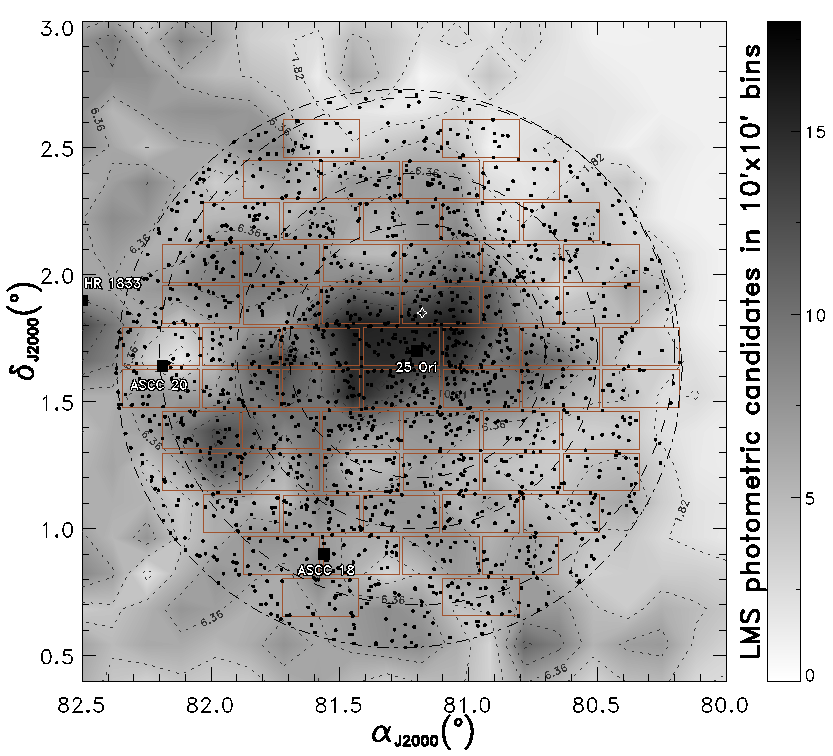
\includegraphics[width=1.0\textwidth]{sky}
	\caption[Spatial distribution of our photometric member candidates.]{Spatial distribution of our photometric member candidates (black points; see Section \ref{sec_IMF:candidates}). The dash-dotted circle shows the FOV of our DECam observations obtained with the array of detectors indicated by the brown boxes. The dashed circles indicate, from the centre outwards, the 25 Ori estimated areas by \citet[0.5$^\circ$ radius; ][]{Downes2014}, \citet[0.7$^\circ$ radius; ][]{Briceno2018} and \citet[1.0$^\circ$ radius; ][]{Briceno2005,Briceno2007} centred at $\alpha_{J2000}=81.2^\circ$ and $\delta_{J2000}=1.7^\circ$. The black squares indicate the labelled stellar groups (25 Ori by \citealt{Briceno2005}, ASCC 18 and ASCC 20 by \citealt{Kharchenko2013} and HR 1833 by \citealt{Briceno2018}). The grey background map indicates the density of LMS and BD photometric member candidates of Orion OB1a in 10'x10' bins \citep{Downes2014}. The white star symbol shows the position of the 25 Ori star.}
	\label{fig_IMF:sky}
\end{figure*}

\subsubsection{CIDA Deep Survey of Orion}
\label{sec_IMF:CDSO}

Additional optical $I_c$-band photometry for sources brighter that the DECam saturation limit (see Section \ref{sec_IMF:sensitivity}) was obtained from the CIDA Deep Survey of Orion \citep[\ac{CDSO}; ][]{Downes2014}. This catalogue was constructed by coading the photometry from the CIDA Variability Survey of Orion \citep[\ac{CVSO}; ][]{Briceno2005,Mateu2012,Briceno2018}, obtained at the National Astronomical Observatory of Venezuela. The area covered by this survey extends beyond the limits of our DECam data.

\subsubsection{VISTA Orion Survey}
\label{sec_IMF:VISTA}
The deep $Z$, $J$ and $K$ near-infrared photometry for this study is from the VISTA survey in Orion \citep{Petr-Gotzens2011}, which was carried out as part of the VISTA science verification program \citep{Arnaboldi2010} with the near-infrared camera (VIRCAM) mounted on the 4.2m telescope at Paranal Observatory.

\subsubsection{Photometry from Literature}
\label{sec:catalogues}
\subsubsubsection{Optical Photometry}
The optical data from DECam and the CDSO were complemented with the $i$-band photometry from the UCAC4 catalogue \citep{Zacharias2013} as well as the $I_c$-band photometry from the $Hipparcos$ catalogue \citep{Perryman1997} for the brightest sources in 25 Ori.

\subsubsubsection{Near-IR Photometry}
We complemented the VISTA near-infrared photometry with $J$ and $Ks$-band photometry from the 2MASS catalogue \citep{Skrutskie2006}.

In Table \ref{tab_IMF:catalogues} we summarized the spatial coverage of 25 Ori (for an area of 0.7$^\circ$ radius, see Section \ref{sec_IMF:spatial}), the spatial resolution and the photometric sensitivities (see Section \ref{sec_IMF:sensitivity}) of the optical and NIR catalogues used in this study. The masses corresponding to the saturation and completeness magnitudes are obtained using the mass-luminosity relation explained in Section \ref{sec_IMF:mass-luminosity}.

\begin{table*}
\caption[Information of the photometric catalogs.]{Spatial coverage of 25 Ori$^1$ and photometric sensitivities of the catalogues used in this study.}
%\begin{center}
  \small
  \label{tab_IMF:catalogues}
  \begin{threeparttable}
 	%\begin{tabular}{@{}p{1.1cm}p{0.5cm}p{0.8cm}cccccp{0.1cm}}
    \setlength{\tabcolsep}{12pt}
 	\begin{tabular}{lcccccccc}
 	\hline
 	\hline
 	Survey      & Phot.    & FWHM      & Area         & Satur.       & Comp.        & Satur.     & Comp.       &  Ref. \\%& Limiting  \\
 	            & Band     & (arcsec)  & [per cent]         & (mag)        & (mag)        & ($M_\odot$)& ($M_\odot$) &       \\%& (mag)     \\
 	\hline
 	DECam       & $I_c$    & 0.9       & $\approx 86$ & 16.0         & 22.50        & 0.16       & 0.012       & a     \\%& 25.0      \\
 	CDSO        & $I_c$    & 2.9       & 100          & 13.0         & 19.75        & 0.86       & 0.020       & b     \\%& 21.5      \\ 
 	UCAC4       & $I_c$	   & 1.9       & 100          & 7.0          & 14.75        & 6.33       & 0.340       & c     \\%& 16.0      \\
 	$Hipparcos$ & $I_c$	   & ---       & 100          & $<$5.0       & ---          & $>$13.5    & ---         & d     \\%& 16.0      \\
 	VISTA       & $J$      & 0.9       & 100          & 12.0         & 20.25        & 0.85       & $<$0.010    & e     \\%& 21.5      \\
 	2MASS       & $J$      & 2.5       & 100          & 4.0          & 16.25        & 19.3       & 0.287       & f     \\%& 17.0      \\
 	\hline
 	\end{tabular}
  \begin{tablenotes}[para,flushleft]
    $^a$Considering an area of $0.7^\circ$ radius.\\
	References: (a) This work; (b) \citet{Downes2014}; (c) \citet{Zacharias2013}; (d) \citet{Perryman1997}; (e) \citet{Petr-Gotzens2011}; (d) \citet{Skrutskie2006}
  \end{tablenotes}
 \end{threeparttable}
\end{table*}

\subsubsection{Merged Optical-NIR Catalog}
\label{sec_IMF:merged_cat}

From the individual catalogues with optical and NIR data we constructed one single general catalogue, as explained in this section.

\subsubsubsection{Transformation of optical photometry into Cousins system}
\label{sec_IMF:photometry_transformation}
We transformed the $i$-band photometry from UCAC4 and DECam to the Cousin system $I_c$-band, which is a photometric band predicted by the BT-Settl \citep{Baraffe2015} and \ac{PARSEC-COLIBRI} \citep{Marigo2017} isochrones used to estimate masses to later construct the system IMF in Section \ref{sec_IMF:mass-luminosity}. To obtain the $I_c$ magnitudes from UCAC4 we used the empirical transformations by \citet{Jordi2006}, which relate SDSS photometry with other photometric systems included the Cousins system. For the DECam photometry we derived directly from our data colour-dependent transformations to convert the calibrated DECam magnitudes to the SDSS system and then to the Cousins system. The RMS we obtained when comparing the $I_c$ magnitudes from the CDSO and those from UCAC4 and from DECam after the transformation are 0.07 and 0.04 mag, respectively. The details about these transformations are described in Appendix \ref{sec_app_IMF:photometry_transformation}. Because the Cousins photometric system is already used by the CDSO and $Hipparcos$ catalogues, after the transformation of the DECam and UCAC4 photometries, the complete sample of optical observations are all in the same photometric system.

\subsubsubsection{Photometric uncertainties}
\label{sec_IMF:photometry_uncertainties}
Before we define the brightness ranges where each catalogue will be used, we fitted exponential functions to the photometric uncertainties of the optical and NIR catalogues with respect to the magnitude ($\delta I_c(I_c)$ for the optical data and $\delta J(J)$ for the NIR data). This way we can estimate the uncertainties of the data as a function of the photometric magnitudes, which will allow us to combine the catalogues considering the typical photometric uncertainties at each brightness point where the catalogues are joined. In Table \ref{tab_IMF:errors} we show the parameters for each catalogue, working with magnitudes inside their saturation and completeness limits (see Section \ref{sec_IMF:sensitivity}).

\begin{table}
\caption[Parameters of the exponentials fitted to the photometric errors of the optical and NIR catalogues.]{Parameters of the exponentials fitted to the photometric uncertainties of the optical and NIR catalogues used in this study.}
  \small
  \label{tab_IMF:errors}
  \setlength{\tabcolsep}{18pt}
  \begin{center}
  \begin{threeparttable}
 	\begin{tabular}{lcccc}
 	%\begin{tabular}{p{0.8cm}p{0.3cm}p{0.5cm}p{0.4cm}p{0.4cm}p{0.4cm}p{0.4cm}p{0.1cm}}
 	\hline
 	\hline
 	Catalog & Photometric &  $a$  &  $b$   & $c$   \\
			& Band        &       &        &       \\
 	\hline
 	DECam   & $I_c$	& 0.005 & 25.861 & 1.042 \\
 	CDSO    & $I_c$	& 0.002 & 22.175 & 0.999 \\
 	UCAC4   & $I_c$	& 0.037 & 8.993  & 0.453 \\
 	VISTA   & $J$	& 0.002 & 16.870 & 0.732 \\
 	2MASS   & $J$	& 0.024 & 20.240 & 1.105 \\
 	\hline
 	\end{tabular}
  \begin{tablenotes}[para,flushleft]
	Note. The exponentials have the form $f(x)=a+e^{(cx-b)}$, where $x$ is the magnitude in the corresponding photometric band.
  \end{tablenotes}
 \end{threeparttable}
 \end{center}
\end{table}

\subsubsubsection{Cutoffs and merged catalogues}
\label{sec_IMF:cutoffs}
The brightness ranges where each photometric catalogue was used are related to their photometric sensitivities, which are described in Section \ref{sec_IMF:sensitivity} and reported in Table \ref{tab_IMF:catalogues}. The $I_c$-band photometry we used to have a combined optical catalogue are as follows: $i)$ UCAC4 for $I_c<13.0+\delta I_c(13.0)$, $ii)$ CDSO for $13.0-\delta I_c(13.0)\leq I_c<17.0+\delta I_c(17.0)$, and $iii)$ DECam for $I_c\geq 17.0-\delta I_c(17.0)$. We also added 25 stars (including 25 Ori) from the $Hipparcos$ catalogue, which are too bright to have $I_c$ magnitudes from UCAC4. The $J$-band photometry used to have a combined NIR catalogue are as follows: $i)$ 2MASS for $J<13.0+\delta J(13.0)$, and $ii)$ VISTA for $J\geq 13.0-\delta J(13.0)$. Then, we removed 3$^{\prime\prime}$ duplicates from the optical and NIR catalogues and kept the sources with smaller photometric uncertainties. To join the optical and NIR catalogues we did a cross-match between them with a tolerance of 3$^{\prime\prime}$ using STILTS\footnote{\url{http://www.star.bris.ac.uk/~mbt/stilts/}} \citep{Taylor2006}.

The final optical and NIR catalogue has 110527 detections inside a FOV of 1.1$^\circ$ radius around the 25 Ori overdensity, being most of them (about 85 per cent) from the DECam and VISTA catalogues.

\subsection{Selection of Photometric Candidates}
\label{sec_IMF:candidates}

\subsubsection{PMS Locus}
\label{sec_IMF:locus}
The use of colour-magnitude diagrams (\ac{CMD}s) combining optical and NIR data has been successfully tested for identifying young stellar objects \citep[e.g. ][ and references therein]{Downes2014}. We selected photometric member candidates from the merged optical and NIR catalogue according to their position in the $I_c$ vs $I_c-J$ digram shown in Figure \ref{fig_IMF:CMD}.

To define the PMS locus in which the member candidates lie, we plotted a large set of 355 spectroscopically confirmed low-mass members of 25 Ori from \cite{Briceno2005,Briceno2007,Downes2014,Suarez2017,Briceno2018} and 15 spectroscopically confirmed very low mass and BD members of 25 Ori and Orion OB1a from \citet{Downes2015}. Most of these members were confirmed through similar spectroscopic procedures, which makes the sample more homogeneous. Additionally to the confirmed members, we also plotted 38 highly probable high-intermediate-mass members from \cite{Kharchenko2005}. The final sample of 408 spectroscopically confirmed members and highly probable members covers the spectral type range from B2 to M9 and trace a clear sequence in the $I_c$ vs $I_c-J$ diagram. This sequence corresponds to the empirical isochrone of 25 Ori, which was defined averaging the $I_c-J$ colours per $I_c$-bin (red dashed curve in Figure \ref{fig_IMF:CMD}). We stress that the resulting empirical isochrone is roughly consistent with the PARSEC-COLIBRI and BT-Settl 7 Myr isochrones. This empirical isochrone was our starting point to define the PMS locus considering the following uncertainties and effects:

$i)$ \emph{Distance uncertainty.} From the sample of spectroscopically confirmed members of 25 Ori, we obtained a mean distance of 356 pc with a standard deviation, \ac{sigma}, of 47 pc, considering the distances reported by \citet[\ac{BJ18}; ][]{Bailer-Jones2018} on the basis of Gaia parallaxes \citep[\ac{Gaia DR2}; ][]{GaiaCollaboration2018}. We considered only distances with uncertainties smaller than 20 per cent (more details in Appendix \ref{sec_app_IMF:distance}). Then, we broaden vertically the edges of the PMS locus in the CMD by adding the 1-$\sigma$ uncertainty in distance, which corresponds to the upwards and downwards offsets of 0.31 and 0.27 mag, respectively.

%$ii)$ \emph{3D distribution of 25 Ori.} Assuming a 25 Ori larger radius of 0.7$^\circ$ \citep{Briceno2018}, which corresponds to 4.3 pc to a distance of 356 pc, we also moved vertically the edges of the locus. \textcolor{blue}{I think it is already included when you add the 1-$\sigma$ uncertainty in the previous step. What do you think?}

$ii)$ \emph{Age uncertainty.} To estimate the change in the $I_c$ brightness ($\Delta I_c$) as a function of the $I_c-J$ colour due to the uncertainty of the 25 Ori age \citep[6.1$\pm$2.4; ][]{Briceno2018}, we worked with the PARSEC-COLIBRI and BT-Settl isochrones. We obtained $\Delta I_c^I$ between the isochrone corresponding to the age of 25 Ori and that for the 25 Ori age minus the error. Similarly, we obtained $\Delta I_c^{II}$ considering the age of 25 Ori and the age plus the error. In most of the colour range considered (-0.5-4.5 mag), $\Delta I_c^I$ is larger than $\Delta I_c^{II}$. We used $\Delta I_c^I$ to move upwards the upper edge of the locus and $\Delta I_c^{II}$ to move downwards the lower edge.

%$ii)$ \emph{Extinction uncertainty.} The objects in the compiled list of confirmed member of 25 Ori have visual extinction derived from spectroscopically obtained spectral types. From these values we obtained a mean extinction of 0.29 mag with a standard deviation of 0.26 mag (see Section \ref{sec_app:extinction}). \textcolor{blue}{" ... considered 1 $\sigma$ uncertainty to move vertically and horizontally the edges of the locus." This is not what you did. You should change this sentence by something like: We considered the effect of extinction on the PMS locus by moving the edges in the direction of a reddening vector with an amplitude of $X$.}

$iii)$ \emph{Unresolved binarity.} According to \citet{Briceno2007}, the observed spread in the CMD of young stars in the 25 Ori field is roughly consistent with the upper limit of 0.75 mag expected from unresolved binaries. Thus, we used this limit to move upward the upper edge of the locus.

$iv)$ \emph{Mean intrinsic variability.} We characterized the $I_c$-amplitude variations as a function of the magnitude for the 25 Ori member candidates from \citet{Downes2014} using the CVSO catalogue. These variations range between 0.2 and 0.9 mag for candidates with $I_c$ magnitudes between 13.0 to 19.0. For brighter and fainter $I_c$ magnitudes we assumed these minimum and maximum variation limits, respectively. Thus, we used these $I_c$-amplitude variations to move upwards and downwards the upper and lower edges of the locus, respectively. For the $J$-band, \citet{Scholz2009} reported the low-level amplitude variations of about 0.2 mag for young LMSs and BDs. Assuming that when occurs a maximum or a minimum in the $I_c$-brightness of a variable source also takes place the maximum or minimum in the $J$-band brightness, we considered $I_c-J$ amplitude variations as the difference between the $I_c$-amplitude variations and the representative 0.2 mag variations in the $J$-band to move leftwards and rightwards the blue (lower) and red (upper) edges of the locus, respectively.

$v)$ \emph{Photometric uncertainties.} We considered the exponentials fitted to the uncertainties of the optical and NIR catalogues as a function of the magnitudes to move both edges of the locus. The upper and lower edges were moved upwards and downwards, respectively, according to the uncertainty corresponding to each $I_c$-magnitude of the optical catalogues used in the different ranges. The blue (lower) and red (upper) edges of the locus were moved leftwards and rightwards, respectively, considering the uncertainties added in quadrature for each $I_c$ and $J$-magnitude from the catalogues used in the different ranges.

The sources lying inside this resulting PMS locus were selected as photometric member candidates of 25 Ori. We selected 1694 candidates inside the DECam FOV having $I_c$ magnitudes from 5.08 to 23.3.

The locus defined this way contains about 93 per cent of the confirmed members and highly probable members of 25 Ori. From the members lying out, on the left side, of the PMS locus, about 75 per cent of them have $>99$ per cent probability of being variable stars in the CVSO. In Section \ref{sec_IMF:missed} we estimated that the fraction of 25 Ori members we can lose in our photometric selection is $\sim3.1$ per cent.

It is important to notice in Figure \ref{fig_IMF:CMD} that in the $I_c$ range roughly between 9 and 13 mag, the giant and subgiant branches cross the PMS locus, which increases the contamination by these sources in this brightness range. We discussed in Section \ref{sec_IMF:fieldcontam} how to deal with this contamination. %We can also see 7 faint sources ($I_c>17$ and $I_c-J>2.9$) lying out, on the red side, of the PMS locus. We checked these 7 sources into the DECam images and found that all of them are affected by the diffraction spikes of nearby bright stars, which explains a fainter $I_c$-band magnitude that produces a redder $I_c-J$ colour.

%These and additional factors should be taking into account before analyzing the mass distribution of the member candidates.

%\textcolor{blue}{We must mention the members placed to the left of the PMS locus. This is very important. I suggest to add the fraction of objects in each case. The diagram could give the feeling that a high fraction of members fall outside the locus.}

\begin{figure*}
	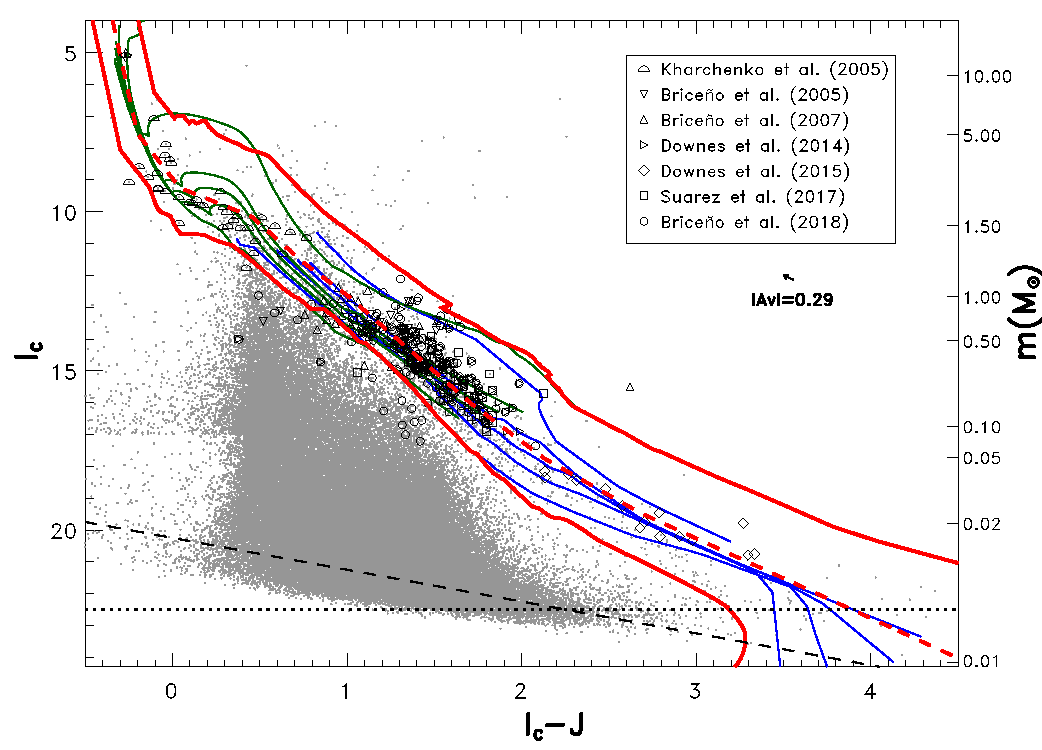
\includegraphics[width=1.0\textwidth]{IvsI-J}
	\caption[$I_c$ vs $I_c-J$ diagram for the selection of the photometric member candidates.]{CMD used for the selection of photometric member candidates of 25 Ori. The red solid curves show the PMS locus defined considering the empirical isochrone (red dashed curve) and several issues that may affect the position of the sources in this plot. The open symbols represent the known spectroscopically confirmed members \citep{Briceno2005,Briceno2007,Downes2014,Downes2015,Suarez2017,Briceno2018} and high-probable members \citep{Kharchenko2005} of 25 Ori, as shown in the label, which trace the empirical isochrone. The grey dots indicate all the detections in our combined optical and NIR catalogue. The black dotted and black dashed lines show the $I_c$/DECam and $J$/VISTA completeness magnitudes, respectively. The blue and green curves indicate, respectively, the BT-Settl and PARSEC-COLIBRI isochrones for ages, from top to bottom, of 1, 5, 7, 10 and 20 Myr. The arrow shows the dereddening vector for the mean extinction of 25 Ori. Masses from the mentioned models for an age of 7 Myr, distance of 356 pc and visual extinction of 0.29 mag are labelled in the right axis. The giants and subgiants branches cross the PMS locus close to (0.9, 13) and (0.5, 11), respectively.}
	\label{fig_IMF:CMD}
\end{figure*}

\subsubsection{Sources of Uncertainty, Contamination and Biases}
\label{sec_IMF:uncertainties}

Several previous works have studied the uncertainties and biases implicit in the observational determination of the IMF \citep[e.g.][]{Moraux2003,Moraux2007a,Moraux2007b,Ascenso2011,Dib2017}. In this section we characterize these effects in the case of 25 Ori and show how we corrected them.

\subsubsubsection{Spatial Completeness}
\label{sec_IMF:spatial}

The CDSO and VISTA catalogues and all the public catalogues considered in this work have a full spatial coverage of the FOV of the DECam observations.

As explained in Section \ref{sec_IMF:DECam}, our DECam observations were obtained with an array of 60 detectors configured as shown in Figure \ref{fig_IMF:sky} (brown boxes), therefore, part of the area in a FOV is lost by the gaps and because the array is not circular. To compute what fraction of a FOV is covered by the DECam data, we used the Monte Carlo method to generate a list of sources randomly distributed inside the FOV and counting those lying inside the detectors. We found this way that for the DECam FOV, the DECam data covers $\approx70$ per cent of the area. If we consider the previously estimated areas of 25 Ori, the DECam observations have a coverage of $\approx 79$ per cent when considering \citet[1.0$^\circ$ radius; ][]{Briceno2005,Briceno2007} and $\approx86$ per cent when considering \citet[0.7$^\circ$ radius; ][]{Briceno2018} or \citet[0.5$^\circ$ radius; ][]{Downes2014}. These fractions will allow us to correct the luminosity function (\ac{LF}) and system IMF of 25 Ori by the spatial coverage of the DECam data. In Table \ref{tab_IMF:catalogues} we report the spatial coverage of 25 Ori for all the catalogues used in this study.

In Table \ref{tab_IMF:candidates} we list the number of member candidates inside the DECam FOV after applying the correction by the spatial coverage of the DECam data. If we had a full coverage of the DECam observations, we would expect 1782 photometric member candidates in the $I_c$ range from 5.08 to 23.3 mag. The mass range corresponding to this brightness range is obtained in Section \ref{sec_IMF:sys-imf}.

\subsubsubsection{Photometric Sensitivity}
\label{sec_IMF:sensitivity}

The saturation and completeness magnitudes for the optical and NIR catalogues were determined, respectively, as the brightest and faintest magnitudes between which the logarithmic number of sources per magnitude bin do not deviate from a linear behaviour. We estimated the masses corresponding to these magnitudes using the BT-Settl and PARSEC-COLIBRI 7 Myr isochrones. In Table \ref{tab_IMF:catalogues} we summarize these values, where we can see how the optical and NIR catalogues complement each other. Therefore, in the determination of the LF and system IMF of 25 Ori, for the sources more massive than the DECam completeness mass (0.012 $M_{Jup}$), it is not necessary to make any correction due to the photometric sensitivity of the catalogues.

\subsubsubsection{Contamination by Field Stars}
\label{sec_IMF:fieldcontam}

Despite the use of optical-NIR CMDs allow a clear selection of young sources, a contamination of $\sim20$ per cent for the low-mass domain \citep{Downes2014} and $\sim30$ per cent for the very low-mass and BD regime \citep{Downes2015} is expected in our sample of photometric member candidates. Furthermore, a higher degree of contamination is expected in the intermediate-mass range of our candidate sample due to giant and subgiant stars.

We estimated the number of field stars inside the PMS locus following two procedures: First, by means of a simulation of the expected galactic stellar population using the Besan\c{c}on Galactic model \citep[hereafter \ac{BGM}; ][]{Robin2003}. Second, empirically, by a fiducial selection of photometric candidates from an observed control field with similar galactic latitude.

For the BGM approach we performed four simulations\footnote{\url{http://model2016.obs-besancon.fr}} in an area of 2x2 deg$^2$ around 25 Ori and considering the photometric uncertainties of our joined optical and NIR catalogues shown in Figure \ref{fig_IMF:errors} and listed in Table \ref{tab_IMF:errors}. The simulated populations combined the optical and NIR photometric errors from UCAC4 and 2MASS (simulation 1), CDSO and 2MASS (simulation 2), CDSO and VISTA (simulation 3), and DECam and VISTA (simulation 4). Then, we joined the resulting simulations by keeping the sources brighter than $I_c=13$ from simulation 1, the sources in the range $13 \le I_c<15$ from simulation 2, the sources with magnitudes $15 \le I_c<17$ from simulation 3, and sources with $I_c \ge 17$ from simulation 4. This way we have a simulated stellar population compatible with our observational joined optical-NIR catalogue.
%\textcolor{blue}{Here you describe precisely how you considered the photometric uncertainties but you didn't explain how you define the remaining parameters the Besan\c{c}on model needs such as distance, steps, extinction etc ... all these quantities need to be included in the text in order to make the process reproducible for the reader.}

\begin{figure}
	\begin{minipage}{0.60\textwidth}
		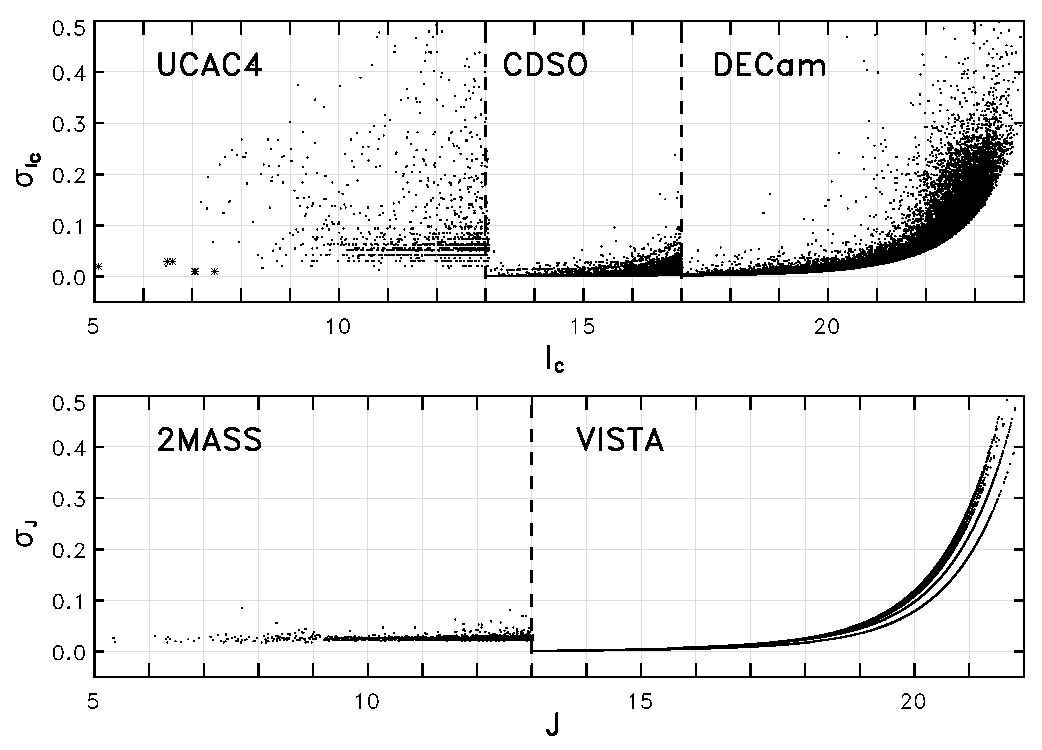
\includegraphics[width=1.00\textwidth]{errors_mix}
	\end{minipage} \hfill
	\begin{minipage}{0.35\textwidth}
		\caption[Photometric uncertainties of the catalogs used for the selection of member candidates.]{Photometric uncertainties as a function of magnitude for the merged optical (top) and NIR (bottom) catalogues. The labelled names indicate the catalogues used in each magnitude range separated by the dashed lines. The few $Hipparcos$ sources in the optical catalogue are indicated by the asterisks.}
		\label{fig_IMF:errors}
	\end{minipage}
\end{figure}

For the control field approach, we estimated the field star contamination in our candidate sample by means of direct counting on selected regions as follows: $i)$ For the optical CDSO, UCAC4 and $Hipparcos$, and NIR 2MASS catalogues, we considered a control field of $1.0^\circ$ radius FOV placed at the same galactic latitude of 25 Ori in a direction moving away from the Orion's Belt ($\alpha_{J2000}= 05^{\rm h} 19^{\rm m} 03^{\rm s}.6$ and $\delta_{J2000} = +04^{\circ} 18' 17''.1$). $ii)$ Since we do not have neither DECam nor VISTA specific observations in this region, we used for these catalogues the areas of the eight north-westernmost and westernmost detectors of the DECam array as control fields, because a) they mostly lie outside the larger estimated area of 25 Ori, b) they have the lesser number of Orion OB1a reported members \citep{Briceno2018,Kounkel2018} and c) the density of LMS and BD candidates in the regions covered by these detectors falls to about 10 per cent of the density in the 25 Ori core \citep{Downes2014}. Then, we joined all the photometric catalogues from both control fields in the same way we did for the 25 Ori observations.

We applied our procedure for selecting photometric member candidates to the BGM and control field samples in order to account the sources lying inside the PMS locus, which we defined as contaminants. When we constructed the $I_c$ distributions of these contaminants in Section \ref{sec_IMF:LF}, we found consistency between the control field and the BGM for magnitudes brighter than $\sim 17$. In Table \ref{tab_IMF:candidates} we list the number of member candidates and contaminants after applying the spatial coverage corrections for the DECam data as well as their complete brightness and mass ranges. We estimated that the fraction of contaminants present in our candidate sample, in the $I_c$ brightness range between 13 and 20 mag, is about 30 per cent, which is somewhat higher than the 20 per cent estimated, and spectroscopically proven, by \citet{Downes2014} in the same brightness range for their candidate selection using similar CMDs. In Section \ref{sec_IMF:sample} we compared both samples. 

As mentioned in Section \ref{sec_IMF:locus} and shown in Figure \ref{fig_IMF:CMD}, there is a high contamination by giant and subgiant stars in the $I_c$ range between $\sim$9 and $\sim$13 mag in our candidate sample. Even, the contaminants estimated by the control field or the BGM can be as numerous as the member candidates in this particular brightness range, which do not allow us to remove the contamination in this range using only the control field or BGM. Fortunately, we can take advantage of Gaia DR2 because in this brightness range all sources have reliable parallaxes. Thus, we did a subset of the member candidates in this peculiar brightness range and having BJ18 distances around the 25 Ori distance and within a dispersion of 1-$\sigma$. Hereafter, we are going to refer to this subset of highly probable 25 Ori members as the distance filtered candidates.

After the correction for the DECam spatial coverage, we have only one BGM contaminant fainter than $I_c=19.6$ mag, while there are about 32 contaminants using the control field in the same brightness range. As the BGM does not include extragalactic sources, this difference between the contaminants counted in both samples suggests than most of the contamination present in the faintest range of our candidate sample is due to extragalactic sources. 

\begin{table}
%\centering\small
\caption[Number of member candidates and contaminants in our sample.]{Number, $I_c$ brightness and mass ranges of the member candidates and contaminants in an area of 1.1$^\circ$ radius around 25 Ori after correcting by the spatial coverage of the DECam data.}
	\small
	\label{tab_IMF:candidates}
    \setlength{\tabcolsep}{12pt}
	\begin{center}
 	\begin{tabular}{@{}lccc}
%	\multicolumn{3}{c}{ \normalsize {Sources Inside the Locus.}}\\
 	\hline
 	\hline
 	Origin  	       & Number            & $I_c$ range  & mass range \\ \vspace{-.05in}
					   & of sources        &              &            \\
 	    	   		   & 	        	   & (mag)        & ($M_\odot$)\\
 	\hline
 	25 Ori FOV         & 1782	  		   & 5.08-23.3    & 0.011-13.1   \\
 	Control Field FOV  & 1030 	  		   & 6.51-23.3    & 0.011-7.74     \\ 
 	BGM                & 840   	  		   & 7.67-19.6$^a$& 0.021$^a$-4.76 \\ 
 	\hline
 	\end{tabular}\\
	$^a$There is a fainter dwarf star contaminant with $I_c=23.5$ (0.011 $M_\odot$).
	\end{center}
\end{table}

\subsubsubsection{Contamination by Extragalactic Sources}
\label{sec_IMF:extgalcontam}

% CCD
As 25 Ori is out of the galactic plane ($b=18.4^\circ$) and has a minimum extinction of 0.29$\pm$0.26 mag, we expect extragalactic sources in any deep photometric sample in that direction. We found in the previous section that the contamination by extragalactic sources dominates the contamination in the faintest range of our member candidate sample. To remove the most likely extragalactic sources from this sample we used the $J-K$ vs $Z-J$ colour-colour diagram (\ac{CCD}) shown in Figure \ref{fig_IMF:CCD}. We plotted a sample of $\approx 500$ spectroscopically confirmed galaxies and quasars in the direction of 25 Ori with $I_c$-brightness between 13.5 and 20.0 mag from \cite{Suarez2017}. Also, we plotted our member candidates and the previously confirmed members of 25 Ori. Similarly than in the CMD, we defined the empirical isochrone traced by the low-mass and BD confirmed members. Then, we defined the sequence centred on this isochrone and containing most than the 90 per cent of the confirmed members. This sequence clearly separates from the region where lie more than the $80$ per cent of the galaxies and quasars. About $1$ per cent (7 sources) of the member candidates plotted in this CCD (those having VISTA photometry) lie in the region defined by the galaxy/quasar sample and have $I_c$ magnitudes between 15.2 and 18.2. We considered these 7 sources as contaminants and removed them from our member candidate sample, keeping the rest of the candidates selected in the CMD. The resultant sample has 1687 member candidates.
%\textcolor{green}{EN ESTE PARRAFO ES IMPORTANTE DECIR SI LAS DIFERENCIAS ENTRE EL CAMPO DE CONTROL Y EL BGM SON CONSISTENTES CON EL NUMERO DE GALAXIAS. LAS 20 QUE REMUEVES SON SOLO EN EL LOCUS.}

In Figure \ref{fig_IMF:CCD}, only three (less than $\sim$1 per cent) of the spectroscopically confirmed members lie in the region where most of the galaxies and quasars lie. Two of these peculiar members are classical T-Tauri stars (\ac{CTTS}s) harbouring circumstellar discs and having an intense H$_\alpha$ emission \citep[41 and 53 \AA; ][]{Suarez2017}, while the other member is a weak T-Tauri star \citep[\ac{WTTS}; ][]{Briceno2007}. These three members are highly probable to be variable stars according to the CVSO, which could explain their position in the CCD.

% Control Field
After we removed from our member candidate sample the potential extragalactic contaminants, we used the control field to statistically remove the extragalactic and galactic contamination from the LF and system IMF of 25 Ori in Section \ref{sec_IMF:LF} and \ref{sec_IMF:IMF}.

\begin{figure}
	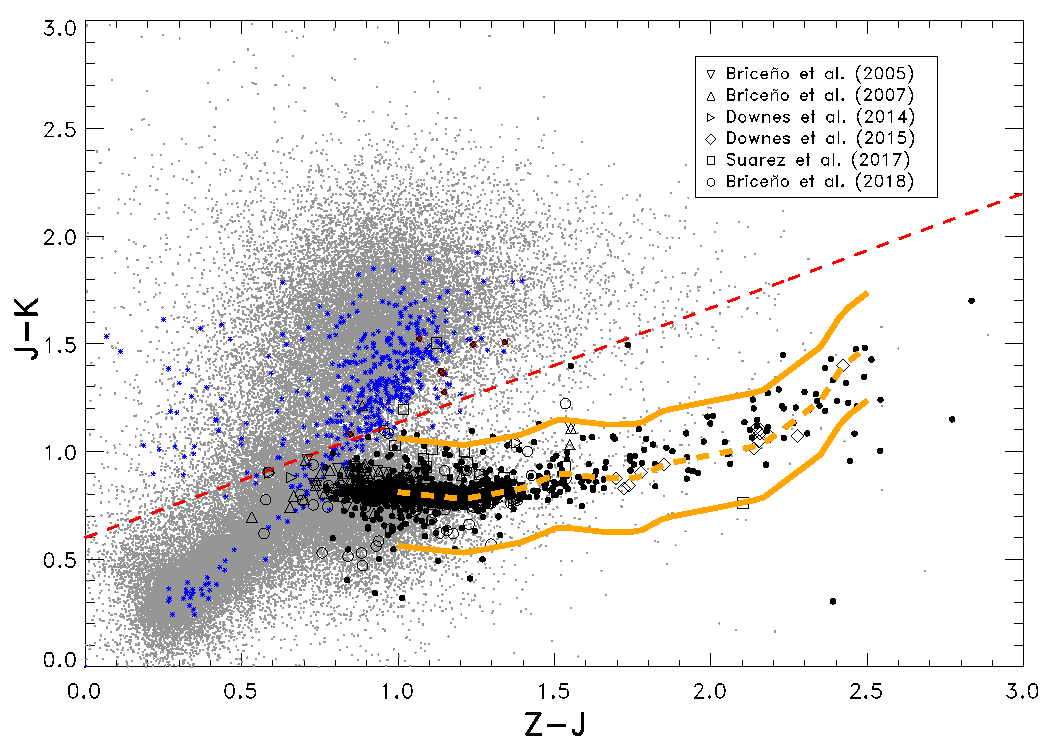
\includegraphics[width=1.00\textwidth]{J-KvsZ-J}
	\caption[$J-K$ vs $Z-J$ diagram to remove potential extragalactic sources in our candidate sample.]{CCD used to remove highly probable extragalactic contaminants (red crosses) from our member candidate sample (black dots). The blue asterisks represent a sample of spectroscopically confirmed galaxies and quasars in the direction of 25 Ori \citep{Suarez2017}. The red dashed line separates more than the 80 per cent of the sample of extragalactic sources from the member candidates. The orange dashed curve shows the empirical isochrone traced by the low-mass and BD confirmed members of 25 Ori by the studies indicated in the label, which are mostly contained in the sequence defined by the orange solid curves. The grey dots are the same as in Figure \ref{fig_IMF:CMD}.}
	\label{fig_IMF:CCD}
\end{figure}

\subsubsubsection{IR excesses}
\label{sec_IMF:excesses}

Possible excesses in the $J$-band, due to discs, can bias the candidate selection because members showing such excesses could lie outside, on the red side, of the PMS locus. In Figure \ref{fig_IMF:CMD} there are 60 sources lying on the right side of the PMS locus, which have $I_c<12.7$ mag. The simulations performed with the BGM show that the positions of these sources are consistent with those of giant stars. Additionally, we checked the distances of these sources and compared them with the currently estimated 25 Ori distance. 97 per cent of the sources with reliable BJ18 distances have values not consistent with those of the 25 Ori members, of which most of them (91 per cent) have larger distances, suggesting these are, in fact, giant stars. Only two sources have distances consistent with 25 Ori, but these sources have unexpected photometric uncertainties from the UCAC4 catalogue (0.146 and 0.234 mag), which could explain, in part, their location in the CMD. Thus, most of the sources left out, on the red side, of the PMS locus are behind the 25 Ori population, indicating that in our photometric selection we do not lose 25 Ori members due to the presence of IR excesses.

Additionally, if the magnitudes used to obtain the masses were affected by the IR excesses, the masses could be overestimated. At the age of 25 Ori, only a fraction of $\sim$5 per cent of the LMSs harbour circumstellar discs \citep{Briceno2005,Briceno2007,Hernandez2007a,Downes2014,Briceno2018}, which produce IR excesses starting at the $WISE\ 3.4\ \mu$m band or longer wavelengths \citep{Suarez2017}. Even for the BDs in 25 Ori, whose have a larger disc fraction of $\sim 30$ per cent, the IR excesses start beyond the $H$-band \citep{Downes2015}. In this study we used the $I_c$ and $J$-band magnitudes which are not expected to be affected by IR excesses. Particularly, we worked with the $I_c$ magnitudes to estimate masses to avoid any overestimation due to IR excesses.

\subsubsubsection{Effects of Chromospheric Activity}
\label{sec_IMF:activity}

Active LMSs suppress the effective temperature (\ac{Teff}) by $\sim5$ per cent and inflate the radius by $\sim10$ per cent with respect to inactive objects \citep[e.g. ][]{Lopez-Morales2007}. These effects roughly cancel themselves, which preserves the bolometric luminosity \citep{Stassun2012}. 

Due to the effective temperature suppression, the masses of active LMSs estimated from the H-R diagram are underestimated, but if masses are estimated from luminosities (or absolute magnitudes), the effect would be much smaller \citep{Jeffries2017}. According to \citet{Stassun2012}, when the effective temperature is used to estimate masses from model isochrones, the resultant masses are systematically lower than the true masses by factors of $\sim3$ and $\sim2$ for LMSs and BDs with intense chromospheric activity of log($L_{H_\alpha}/L_{bol})=-3.3$, respectively. This level of chromospheric activity corresponds to the saturation limit in young LMSs, which separates the CTTSs from WTTSs \citep{BarradoYNavascues-Martin2003}. For LMSs and BDs with low levels of magnetic activity (log($L_{H_\alpha}/L_{bol})=-4.5$), the masses estimated using the effective temperature are systematically lower than true values by factors of $\sim2$ and $\sim1.5$, respectively. Instead, when masses are estimated using the bolometric luminosity derived from the $K$-band absolute magnitudes and considering model isochrones, the resulting masses are $\sim5$ per cent smaller than true values for LMSs and BDs with high chromospheric activity and roughly unaffected for LMSs and BDs with low chromospheric activity.
%% avoid hyperlink error
%\\ \\

In our case, as explained in Section \ref{sec_IMF:mass-luminosity}, we obtained the masses of the member candidates using absolute magnitudes and model isochrones, which minimize the bias in the mass determination of active stars. Additionally, the fraction of active stars in 25 Ori is $\sim 5$ per cent \citep[][]{Briceno2005,Briceno2007,Hernandez2007a,Downes2014,Briceno2018}. Considering the expected $\sim$5 per cent underestimation of masses for the expected $\sim$5 per cent of active stars in our candidate sample, we estimated that the change in the system IMF of 25 Ori is smaller than the Poisson noise of the distribution.

\subsubsubsection{Spatial Resolution and Binaries}
Most of the mass distributions of stellar clusters available in the literature do not take into account unresolved binaries or multiple systems and are, in fact, the system IMFs \citep[e.g. Table \ref{tab_IMF:imf_literature} and ][]{Bastian2010}.

A revision and treatment of the effect of unresolved binary systems in the IMF parametrization is found in \citet{Muzic2017}. They found that the mass distribution becomes steeper in the low-mass and high-mass sides when correcting the system IMF by binary systems to obtain the single-star IMF, but the changes in the slopes agree within the uncertainties. A similar effect on the IMF due to binary systems is reported in \citet{Kroupa2001b}.

In this study we reported the system IMF of 25 Ori, which will allow us to directly compare it with all the system IMFs in Table \ref{tab_IMF:imf_literature}, assuming that the binarity properties are similar for these populations and a similar spatial resolutions of the data used in the different studies. The conversion of the 25 Ori system IMF to the single-star IMF is beyond the scope of this study.

\subsubsubsection{Estimation of the Missed Members}
\label{sec_IMF:missed}
As explained in the previous sections, in our estimation of the system IMF we corrected the possible over-counting of individual stars and/or stellar systems belonging to 25 Ori by considering several sources of contamination in the photometric sample. An additional improvement of our procedure is to estimate possible under-counting of members by estimating the number of 25 Ori individual stars and/or stellar systems that could lie outside the PMS locus defined in the CMD.

We made this estimation through a simple simulation of the expected distribution of the cluster members in the $I_c$ vs $I_c-J$ diagram and computing the fraction of these that falls outside the PMS locus. The simulation was performed as follows, in which we refer as \emph{synthetic members} to those individual stars and/or stellar systems obtained from a realization of the system IMF:

$(i)$ We made a random realization of the 25 Ori system IMF by drawing masses for 1700 synthetic members from a lognormal distribution with $m_c=0.31$ and $\sigma=0.46$. These parameters matches the number of 25 Ori candidates in our sample as well as the resulting system IMF that will be discussed in Section \ref{sec_IMF:parametrizations}. 

$(ii)$ The $I_c$ and $J$-band absolute magnitudes of each synthetic member were computed by interpolating their masses into the mass-luminosity relation using the 7 Myr isochrones of BT-Settl and PARSEC-COLIBRI, as explained in Section \ref{sec_IMF:mass-luminosity}.

$(iii)$ The absolute magnitudes were converted into apparent magnitudes by adding the distance moduli and the corresponding extinctions. The distances and extinctions were generated for each synthetic member by creating random realizations considering the inversion of the cumulative distributions of the BJ18 distances and visual extinctions from spectroscopically confirmed members of 25 Ori (see Figure \ref{fig_IMF:cum_dist}). Visual extinctions were converted into extinctions in $I_c$ and $J$ bands through the \cite{Rieke-Lebofsky1985} extinction law with $R_V$=3.02.

$(iv)$ We randomly labelled $25$ per cent of the synthetic members as photometrically variables in both $I_c$ and $J$ bands. To each of the variables we assigned a variation, $\Delta I_c$, drawn at random from a normal distribution with zero mean and standard deviation, $\sigma _{I_c}$, equal to 0.3. The fraction of variables as well as $\sigma _{I_c}$ were obtained by matching the catalogue of member candidates with the CVSO, which includes stars and BDs with K and M spectral types. A total of 840 candidates ($\sim$50 per cent of the candidate sample) fainter than $I_c=13$ mag (saturation of the CVSO) have a counterpart in the CVSO and we considered as variable the 220 candidates having a probability $>99$ per cent of being variables in the $I_c$-band. The $J$-band variation was computed by multiplying the $\Delta I_c$ by the ratio between the amplitude variations in the $I_c$ and $J$-bands from \cite{Scholz2009}. Both variations were added to the corresponding apparent magnitudes computed in $(iii)$.

$(v)$ We assumed no IR excesses in the $J$-band because at the 25 Ori age they are observed at larger wavelengths, as explained in Section \ref{sec_IMF:excesses}.

$(vi)$ Finally, we simulated the photometric uncertainties in the $I_c$ and $J$-bands by adding to the corresponding apparent magnitude a random error based on an estimation of the photometric errors present in our data. Such estimations were obtained through the fit we did to the mean errors as a function of the mean magnitudes and a fit of the standard deviation of errors as a function of the mean magnitude. Then, for each source, the final apparent magnitude is computed by extracting a magnitude from a normal distribution which is centred at the mean apparent magnitude resulting from $(v)$ with a standard deviation equal to the standard deviation of errors that corresponds to such mean apparent magnitude.

We generated 1000 random realizations of the cluster and obtained that a mean fraction of $\sim3.1$ per cent of the synthetic members fall outside the PMS locus, with most of them ($\sim3.0$ per cent) lying on the left side. We found that this fraction and distribution are consistent with the fraction of confirmed members lying outside the PMS locus shown in Figure \ref{fig_IMF:CMD}. In Figure \ref{fig_IMF:syntheticIvsIJ} we show the result of a characteristic simulation.

Through the variation of the input parameters within values representative of 25 Ori, we found that the main effects that can move synthetic members outside the PMS locus is the photometric variability. As expected, within reasonable values, the system IMF parameters $m_c$ and $\sigma$ do not affect the number of synthetic members falling outside the PMS locus, so our estimation of the under-counting is not affected by the assumed system IMF.

\begin{figure}
	\begin{minipage}{0.60\textwidth}
		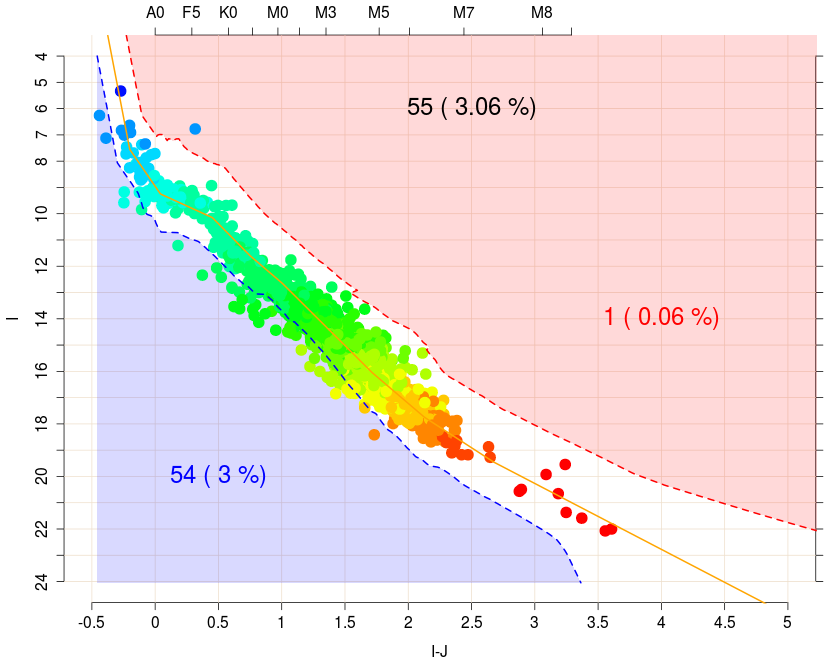
\includegraphics[width=1.00\textwidth]{CMD_simulator.png}
	\end{minipage} \hfill
	\begin{minipage}{0.35\textwidth}
		\caption[Simulated $I_c$ vs $I_c-J$ diagram to estimate missed members in our sample.]{Simulated $I_c$ vs $I_c-J$ diagram for the estimation of the number of members missed by our candidate selection procedure. Dashed lines indicate the PMS locus and solid line the empiric isochrone. The number and fraction in the top of the plot indicate the missed members in both sides of the PMS locus, as indicated in the labels, considering the 1700 synthetic members. The colored scale indicates the mass of the synthetic members.
	%    {\bf deberia tener una escala de colores a la derecha. Update figure with the empirical isochrone.} 
		\label{fig_IMF:syntheticIvsIJ}}
	\end{minipage}
\end{figure}

\subsubsection{Resulting Sample of Member Candidates}
\label{sec_IMF:sample}
The resultant sample selected from the PMS locus in the CMD and after removing potential extragalactic contaminants in the CCD has 1687 photometric member candidates with $I_c$ magnitudes between 5.08 and 23.3 ($0.011-13.1\ M_\odot$) and covering an area of 1.1$^\circ$ radius around 25 Ori. The completeness of this sample is at $I_c=22.5$ mag ($12\ M_{Jup}$) and the brightest sources in 25 Ori are also included. For a statistical removal of the field star and extragalactic contaminants in this sample, when constructing the LF and system IMF in Sections \ref{sec_IMF:LF} and \ref{sec_IMF:sys-imf}, respectively, we used the control field and, as a comparison for the galactic contamination, the BGM. The contamination present in our sample depends of the brightness range but it can be roughly characterized into three ranges. The extragalactic contamination starts to be significant for $I_c$ magnitudes fainter than $\sim$17 mag. For the bright $I_c$ range, between $\sim$9 to 13 mag, there is a high level of contamination by giant and subgiant stars (reason why we did a subset of the sample filtered in distance). In the brightness range between these kind of contaminants, the PMS population is clearly distinguished from the old dwarf stars and the contamination decreases. We estimated, using the control field and/or the BGM, a contamination of $\sim20$ per cent in our sample in the range between 13 and 17 mag. Actually, in this brightness range is where most of the 25 Ori members has been spectroscopically confirmed, as show in Figure \ref{fig_IMF:CMD}.

With our sample we confirmed the low density in 25 Ori. We obtained a stellar density of 8.6 to 4.8 stars/pc$^3$ for the areas of 0.5 and 1.0$^\circ$ radius, respectively, while the substellar density goes from 1.3 to 0.7 BDs/pc$^3$ for the same areas, considering the 25 Ori distance estimated in this study. This stellar density values are roughly consistent with \citet{Briceno2007,Downes2014,Briceno2018}.

% Comparison of our sample with the one from Downes+ (2014).
We compared our candidate sample with the candidate selection done by \citet{Downes2014} using a similar procedure and the CDSO and VISTA catalogues. Their sample includes candidates with masses in a smaller range ($0.02\le M/M_\odot\le0.80$) but covering a larger area (about 3x3 deg$^2$ around the 25 Ori overdensity). If we consider the same area as in the present work, there are about 750 candidates in their selection. Our sample contains 924 member candidates in the same mass range and includes 91 per cent of their candidates. More than a half of their candidates not included in our sample and with $I_c>17$ mag (brightness limit from which we used the DECam photometry) lie within the gaps of the DECam array. Thus, where we have full spatial coverage, we recover more than 96 per cent of the member candidates by \citet{Downes2014} and, additionally, we reported 242 new candidates in the same mass range covered by their study. We estimated that the contamination in our candidate sample, in the $I_c$ brightness range between 13 to 20 mag, is about 30 per cent, which is somewhat higher than the 20 per cent estimated and spectroscopically proven by them in their sample. This difference is due, mainly, because our PMS locus is somewhat wider.

\subsection{Results and Discussion}
\label{sec_IMF:results}

\subsubsection{Luminosity Function}
\label{sec_IMF:LF}

In order to construct the LF is necessary to have absolute magnitudes. The absolute magnitudes we estimated here correspond to the consideration that the member candidates and contaminants are real members of 25 Ori. Thus, these absolute magnitudes are fiducial, though for those candidates being true 25 Ori member they should be close to the real ones. Despite this consideration, these absolute magnitudes allow us to analyse properties of the candidate sample as a whole, as the LF and the system IMF.

For the member candidate sample we worked with the $I_c$-band photometry. Additionally, it is also necessary to estimate distance and extinction values for each member candidate because we do not have these values for the whole sample; 86 per cent of the sample has reliable BJ18 distances and only 18 per cent of the candidates (those spectroscopically confirmed as members) have extinctions from previous studies. From a list of 334 spectroscopically confirmed members of 25 Ori \citep{Briceno2005,Briceno2007,Downes2014,Downes2015,Suarez2017,Briceno2018}, we constructed the normalized cumulative distributions of their BJ18 distances and reported extinctions. We used the inversion of these observed distributions to create random realizations to assign values of these parameters to each member candidate, even those already having reliable Gaia DR2 parallaxes or extinctions from previous spectroscopic studies, in order to have a sample with all values consistent with those from the 25 Ori members. A detailed explanation of this procedure is found in Appendix \ref{sec_app_IMF:distance_extinction}. With these distances and extinctions, together with the $I_c$ photometry, we computed the corresponding absolute magnitudes, $M_{I_c}$, for all the member candidates. We made $10^4$ repetitions of this experiment in order to obtain a robust simulation, which produced $10^4$ artificial distributions in the $M_{I_c}$ range from -2.8 to 15.4 mag. Additionally, we obtained in a similar way $10^4$ $M_{I_c}$ magnitudes for each candidate in the distance filtered subset. The resultant $M_{I_c}$ range of this subset goes from $\sim 1$ to $\sim 5$ mag, assuming the distance and extinction of 25 Ori, and corresponds to the region mostly affected by giant and subgiant stars.

For the contaminants from the control field and BGM, we estimated their fiducial $M_{I_c}$ magnitudes following the same procedure we used for the member candidates. This way we can estimate the contamination in the $M_{I_c}$ distribution of the member candidates to obtain the LF.

Using the simulation just described, we constructed the $10^4$ $M_{I_c}$ distributions of the member candidates and contaminants. To correct each distribution of the candidates by the spatial coverage factor of DECam, we first made the $M_{I_c}$ distribution of the candidates from this catalogue to apply the correction and then we added the distribution of the rest of the data. We constructed in a similar way the $M_{I_c}$ distributions of the contaminants in the control field.

%\textcolor{green}{EN EL SIGUIENTE PARRAFO LO RELEVANTE ES LA ULTIMA FRASE. LO ANTERIOR SE PUEDE QUITAR PUES YA LO DIJISTE.}
With the $10^4$ $M_{I_c}$ distributions of the member candidates and contaminants, we defined the distributions using the mean values and assigning uncertainties of 1 $\sigma$. The resultant distribution of the contaminants from the control field and the BGM are consistent within the uncertainties for $M_{I_c}$ magnitudes brighter than $\sim 9$, even where the giant and subgiant stars lie, which indicates that the contamination in our sample in this range is due mainly to field stars. For fainter sources, a significant discrepancy arises between both samples of contaminants, which increases with the magnitude value, suggesting the presence of extragalactic sources. We decided to work with the contaminants estimated from the control field, because this also allow us to remove these extragalactic sources.

To the $M_{I_c}$ distribution of the member candidates we subtracted the distribution of the contaminants in the control field and by adding the errors in quadrature. In the resultant distribution we replaced the $M_{I_c}$ interval ($\sim1-5$ mag) containing a high giant and subgiant star contamination by the distribution of the candidates in the distance filtered subset, which results in the LF of 25 Ori.

We constructed LFs for different FOVs starting with a radius of $1.1^\circ$ and decreasing it by steps of $0.1^\circ$ until having a radius of $0.5^\circ$ (the 25 Ori overdensity). In Figure \ref{fig_IMF:LF} we show the LFs for the 25 Ori estimated areas. These LFs have very similar morphologies, within the uncertainties.

\begin{figure*}
	\centering
	\begin{tabular}{ccc}
		\subfloat{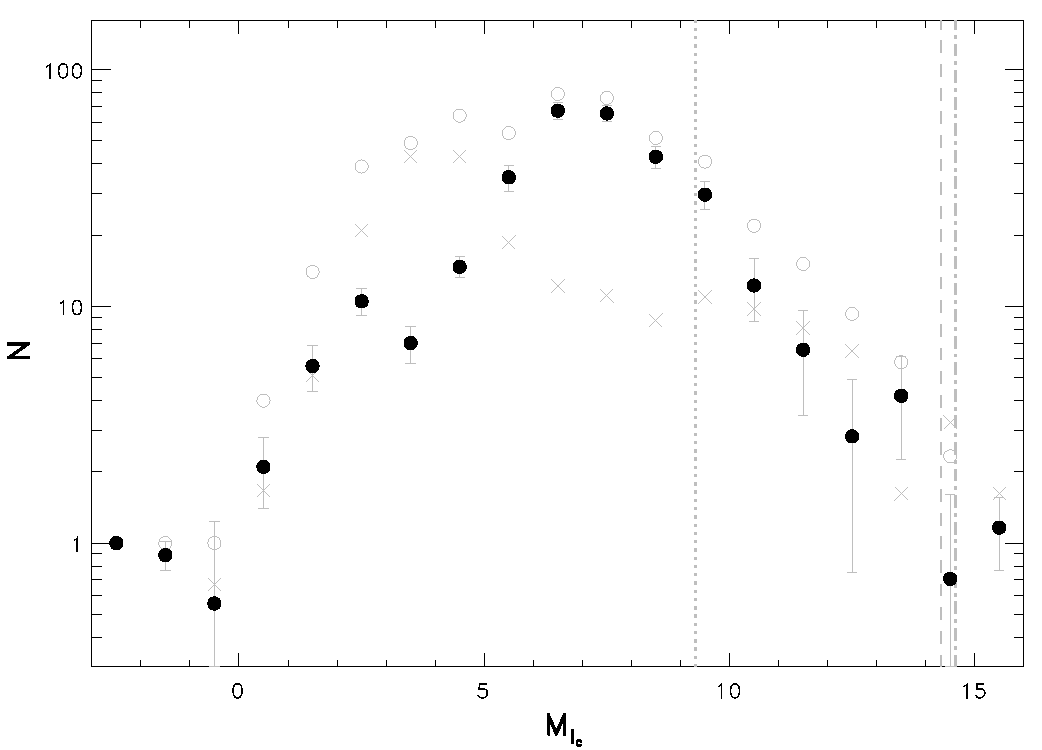
\includegraphics[width=.33\linewidth]{LF_FOV_0-5deg.pdf}} & 
		\subfloat{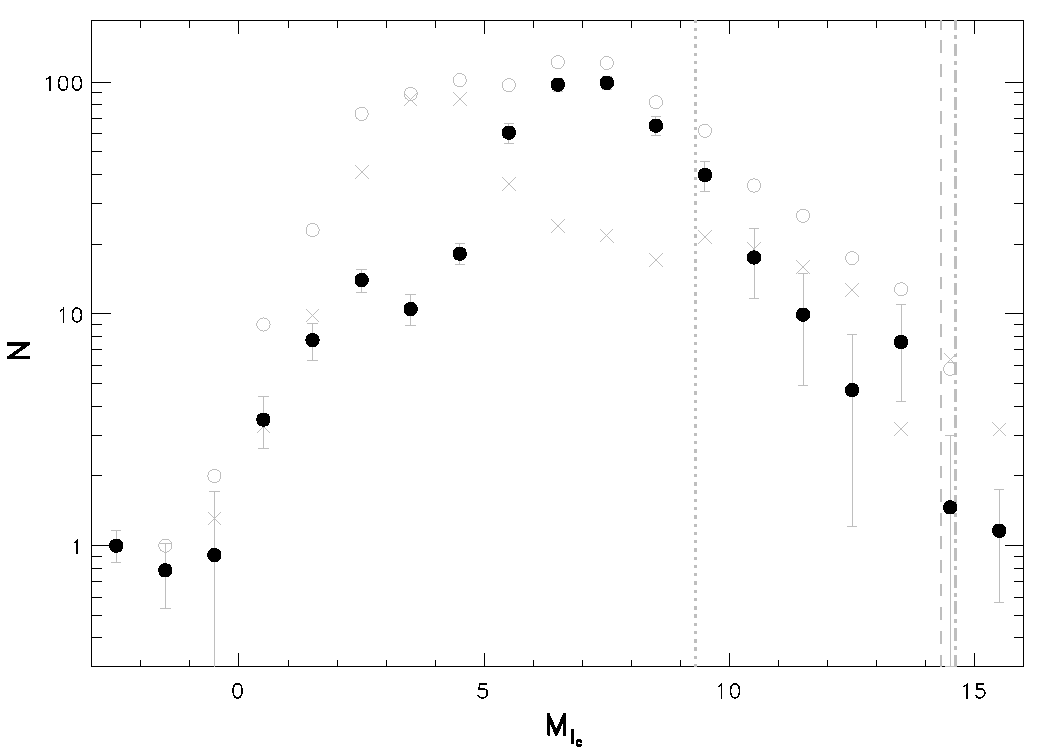
\includegraphics[width=.33\linewidth]{LF_FOV_0-7deg.pdf}} &
		\subfloat{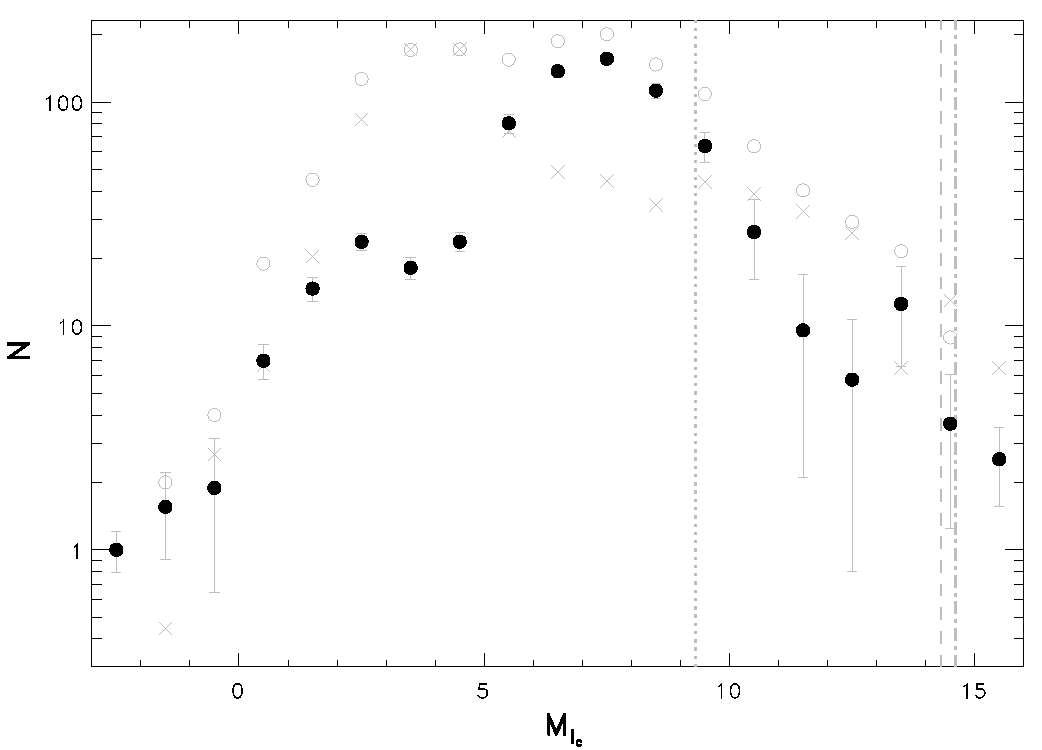
\includegraphics[width=.33\linewidth]{LF_FOV_1-0deg.pdf}}
	\end{tabular}
	\caption[LFs for the 25 Ori areas.]{LFs after correcting by the galactic and extragalactic contamination (grey crosses) in our member candidate sample (grey open circles) inside the 25 Ori estimated areas. The panels from left to right correspond to the areas by \citet[0.5$^\circ$ radius; ][]{Downes2014}, \citet[0.7$^\circ$ radius; ][]{Briceno2018} and \citet[1.0$^\circ$ radius; ][]{Briceno2005,Briceno2007}. The vertical lines, from left to right, indicate the substellar limit (H burning limit), the BD-planetary object limit (D burning limit) and the completeness limit of our DECam observations.
	\label{fig_IMF:LF}}
\end{figure*}


\subsubsection{System IMF}
\label{sec_IMF:IMF}
The main purpose of this study is to determine the system IMF of 25 Ori. Therefore, we need to estimate through a mass-luminosity relationship, the corresponding masses for our member candidates and contaminants under the consideration they are true members of 25 Ori.

\subsubsubsection{Mass-Luminosity Relationship}
\label{sec_IMF:mass-luminosity}

At the age of 25 Ori \citep[7-10 Myr; ][]{Briceno2005,Briceno2007,Downes2014,Briceno2018}, stars with masses between $\sim 2$ and $\sim 15\ M_\odot$ should be already in the MS, while less massive objects are still in the PMS and more massive stars are in post-MS stages \citep[][]{Prialnik2000}. The most massive star in 25 Ori is the star with the same name, classified as a peculiar B1V star with broad lines \citep{Houk1999}, which roughly corresponds to $\sim 10\ M_\odot$ using the \citet{Schmidt-Kaler1982} empirical mass-luminosity relationship. Therefore, we do not expect in our candidate sample members of 25 Ori being in post-MS but we do expect PMS and MS members. We estimated that $\sim7$ per cent of our candidates have masses larger than 2 $M_\odot$, considering the system IMF by \citet{Downes2014}.

In order to cover the large $M_{I_c}$ range in our candidate sample (from -2.8 to 15.4 mag), we worked with two sets of mass-luminosity relationships for PMS and MS stellar models at the age of 25 Ori. We considered the 7 Myr isochrones of PARSEC-COLIBRI for masses higher than $1.0\ M_\odot$ and of BT-Settl for lower masses. These isochrones were obtained assuming solar metallicity. In Figure \ref{fig_IMF:mass-L} we show the resulting mass-luminosity relation from high-mass stars to very low-mass objects (from 0.01 to 15 $M_\odot$). We stress the soft transition between both isochrones at the selected cutoff at 1$M_\odot$. 

If instead of these 7 Myr isochrones we consider those of 10 Myr (the older quote of the 25 Ori age), the resultant mass-luminosity relations look very similar, only showing differences smaller than $\sim 30$ per cent in the $M_{I_c}$ range from 9 to 11 mag, as shown in Figure \ref{fig_IMF:mass-L}.

\begin{figure}
	\begin{minipage}{0.60\textwidth}
		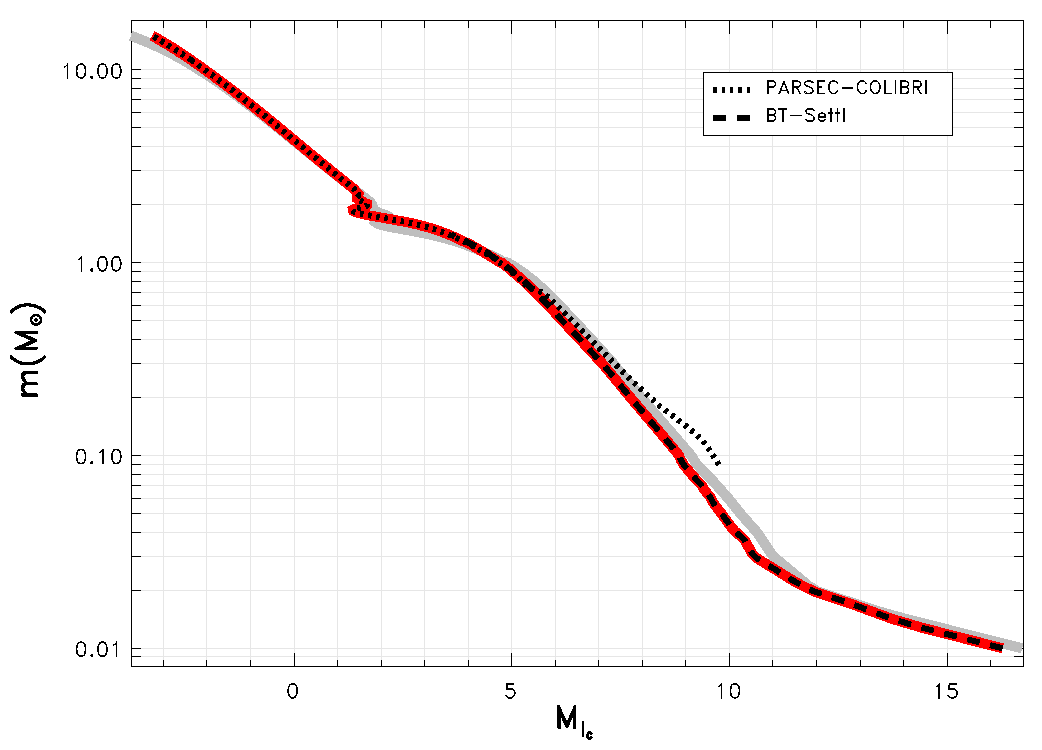
\includegraphics[width=1.00\textwidth]{mass-MIc}
	\end{minipage} \hfill
	\begin{minipage}{0.38\textwidth}
		\caption[Mass-luminosity relation for estimating masses.]{Mass-luminosity relation used to estimate the masses of the member candidates and contaminants (red solid curve). This relation is a combination of the 7 Myr isochrones of BT-Settl and PARSEC-COLIBRI, which are indicated by the dashed curve and the dotted curve, respectively. The mass-luminosity relation considering instead the 10 Myr isochrones is represented by the grey solid curve, which is mostly contained into the thickness of the mass-luminosity relation for 7 Myr.}
		\label{fig_IMF:mass-L}
	\end{minipage}
\end{figure}

\subsubsubsection{System IMF Determination}
\label{sec_IMF:sys-imf}

By interpolation of the $M_{I_c}$ magnitudes into the mass-luminosity relationship explained in the previous section, we estimated the masses that correspond to each member candidate as well as to each contaminant considering they are members of 25 Ori. As we have $10^4$ $M_{I_c}$ values for each source, we obtained $10^4$ masses for each source. The resulting mass range covered by the member candidates goes from $0.011$ to 13.1 $M_\odot$. In Table \ref{tab_IMF:candidates} we list this mass range along with those for the samples of contaminants.

With these masses we constructed the mass distributions of the member candidates and contaminants. Similarly than for the $M_{I_c}$ distributions, we corrected the distributions by the spatial completeness of DECam and then we defined the mass distribution using the mean values and assigning errors of 1 $\sigma$. From the mass distribution of the member candidates we subtracted that of the control field contaminants adding the errors in quadrature. Then, we replaced in the resulting distribution, to refine the removal of giant and subgiant star contamination, the range between $\sim$0.9 and 3 $M_\odot$ by the mass distribution of the candidates in the distance filtered subset. The resultant distribution corresponds to the system IMF of 25 Ori, which is complete from 12 $M_{Jup}$ to 13.1 $M_\odot$ (corresponding to the 25 Ori star).

%\textcolor{green}{ESTE PARRAFO TIENE VARIOS PROBLEMAS: 1) NO PUEDES DECIR "WE CAN SEE" PORQUE LA FIGURA NO TE DEJA VER LA INCOMPLETITUD. 2) NO ENTIENDO DE DONDE SALE EL NUMERO DE FUENTES ESPERADAS PARA CALCULAR EL 1.5. 3) EL BIN MENOS MASIVO NO NECESITA SER MENCIONADO PORQUE NO FORMA PARTE DE LA DISCUSION. YA MENCIONASTE A LOS OBJETOS QUE CAEN ALLI. 4) NO ENTIENDO DE DONDE SACAS QUE SE ESPERAN 100 CANDIDATOS A FFP. EL NUMERO ESPERADO ES DE ENTRE 3 Y 5 SEGUN LAS SIMULACIONES.}
In Figure \ref{fig_IMF:imf} we show the system IMFs for the 25 Ori estimated areas. The least massive bin (at log $m=-1.9$) is partially affected by the completeness of our DECam data. We corrected the counts of this bin by a factor of $\sim2.5$, resulting from the ratio between the number of expected sources and those observed in DECam. 
%The factor to correct the least massive bin, which includes planetary-mass objects, is $\sim 50$, but as this bin is completely out of our photometric sensitivities, we did not correct it. However, considering this correction factor and that these two candidates are members of 25 Ori, we roughly expect 100 free-floating planets (substellar objects with $m\lesssim10\ M_{Jup}$) in 25 Ori.

\begin{figure*}
	\centering
	\begin{tabular}{ccc}
		\subfloat{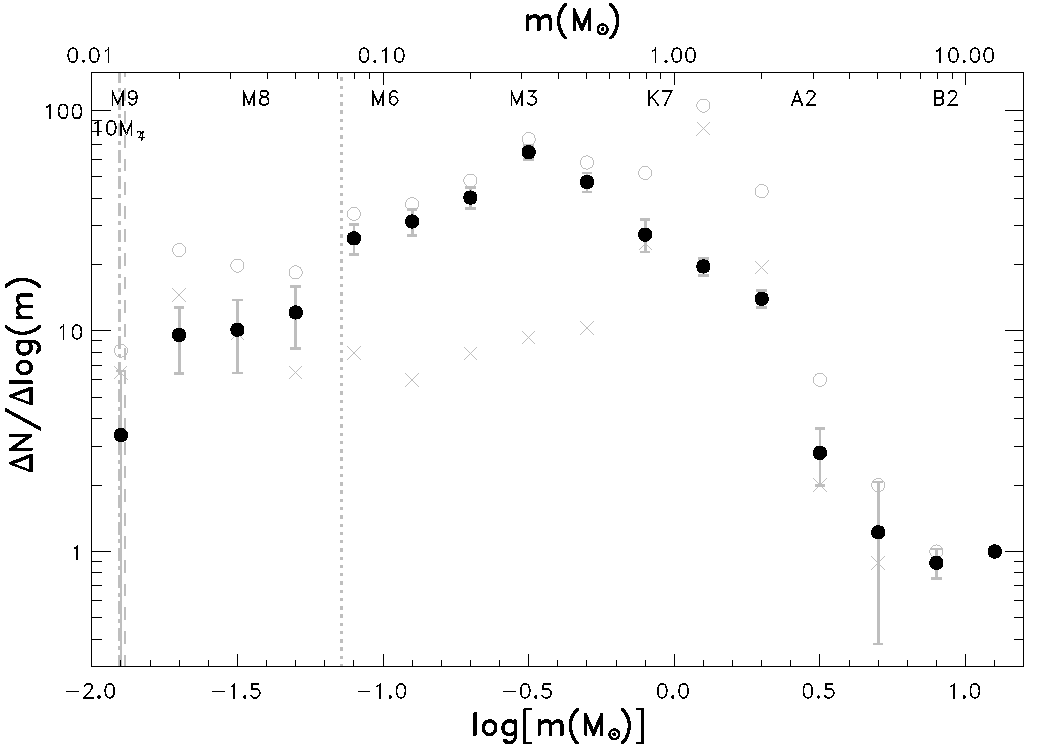
\includegraphics[width=.33\linewidth]{IMF_FOV_0-5deg.pdf}} & 
		\subfloat{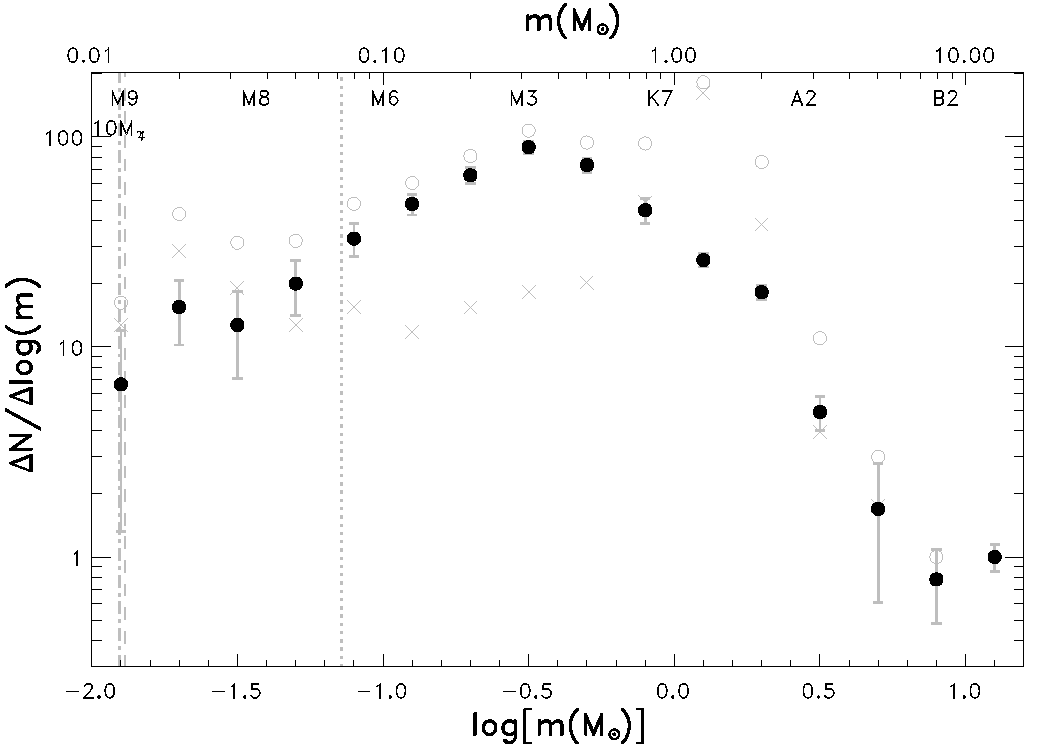
\includegraphics[width=.33\linewidth]{IMF_FOV_0-7deg.pdf}} &
		\subfloat{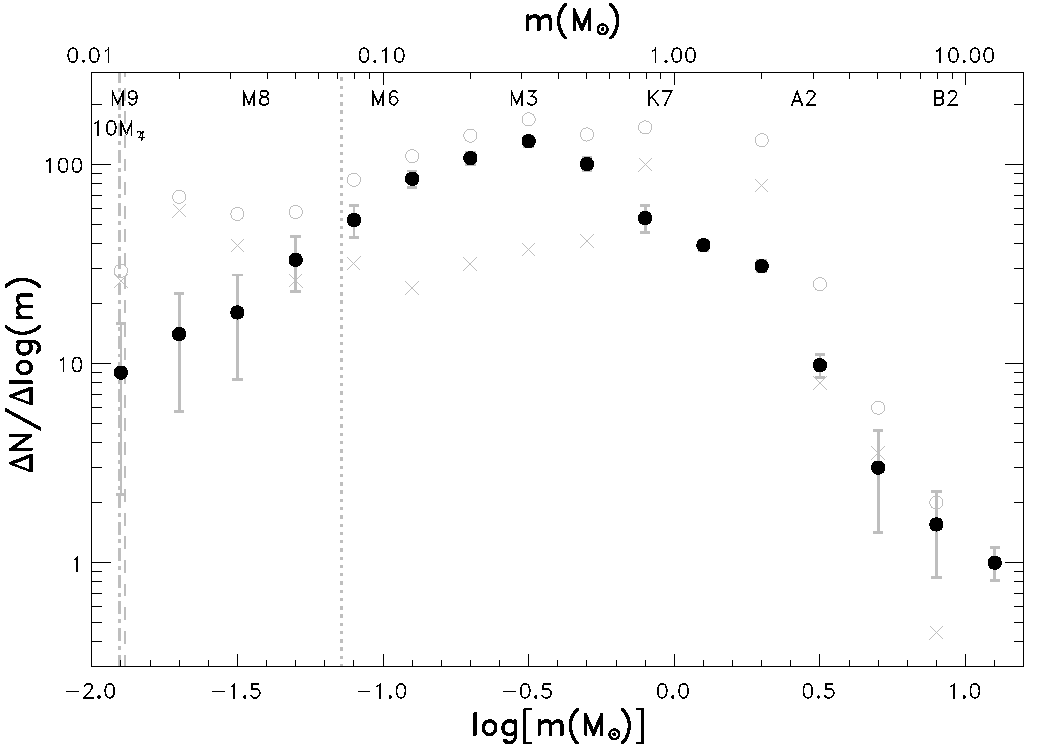
\includegraphics[width=.33\linewidth]{IMF_FOV_1-0deg.pdf}} 
	\end{tabular}
	\caption[25 Ori system IMFs]{System IMFs of 25 Ori after correcting by the galactic and extragalactic contamination (grey crosses) in our member candidate sample (grey open circles). The panels, from left to right, correspond to the 25 Ori areas by \citet[0.5$^\circ$ radius; ][]{Downes2014}, \citet[0.7$^\circ$ radius; ][]{Briceno2018} and \citet[1.0$^\circ$ radius; ][]{Briceno2005,Briceno2007}. The vertical lines are the same as in Figure \ref{fig_IMF:LF}. The size of the bin is 0.2 dex.
	\label{fig_IMF:imf}}
\end{figure*}

\subsubsubsection{Parametrizations}
\label{sec_IMF:parametrizations}

We described the derived system IMF of 25 Ori using the following parametrizations:

%\textcolor{green}{SUMA LAS REFERENCIAS A LAS ECUACIONES. KROUPA, CHABRIER Y DE MARCHI. NOTA QUE EN LAS DOS PRIMERAS ELLOS SON QUIENES DEFINEN LOS RANGOS DE AJUSTE Y EN LA TERCERA ES DE MARCHI QUIEN INTRODUCE LA PARAMETRIZACION. CREO QUE ES IMPORTANTE INCLUIR A PARRAVANO EN ESTAS ULTIMAS REFERENCIAS.}

$i)$ A triple power-law distribution in the form:

\begin{equation}
	\xi(\log m)\propto m^{-\Gamma_i}
\end{equation}

with $\Gamma_1$, $\Gamma_2$ and $\Gamma_3$ for the mass ranges $m\le0.30\ M_\odot$, $0.30<m/M_\odot<1$ and $m\ge1\ M_\odot$, respectively. Such parametrization is inspired by that for the Galactic-field IMF proposed by \citet{Kroupa2001b,Kroupa2002}, but with different break masses because his IMF is defined when resolving multiple systems.

$ii)$ A lognormal distribution for masses $m\le1M_\odot$, according to \citet{Chabrier2003a,Chabrier2003b}:

\begin{equation}
\xi(\log m)\propto e^{-\frac{(\log m-\log m_c)^2}{2\sigma^2}}
\end{equation}

where \ac{mc} is the characteristic mass and $\sigma$ the standard deviation. If we consider the lognormal fit up to 13.1 $M_\odot$, the resultant parameters are in agreement, within the errors, with those when the fit is done for masses $m\le1M_\odot$.

$iii)$ A tapered power-law function for the whole mass range of the system IMF ($0.012-13.1\ M_\odot$):

\begin{equation}
\xi(\log m)\propto m^{-\Gamma} \Big[1-e^{-(m/m_p)^\beta}\Big]
\end{equation}

where $m_p$ is the peak mass, $\Gamma$ the power law index and $\beta$ the tapering exponent. This function, introduced by \citet{DeMarchi2005}, has a power law behaviour for high masses and an exponential truncation for lower masses.

In Figure \ref{fig_IMF:imf_par} we show these functions fitted to the 25 Ori system IMF and in Table \ref{tab_IMF:imf} we summarize the parameters with their uncertainties. In these fits we avoided the most massive bin(s) with counts lesser than the unity because they are at the noise level. The reason why we have counts lesser than one is because to the member candidate mass distribution we subtracted the mass distribution of the contaminants after applying the correction by the spatial coverage, which can result in a fractional number.

\begin{figure*}
	\centering
	\begin{tabular}{ccccccccc}
		\subfloat{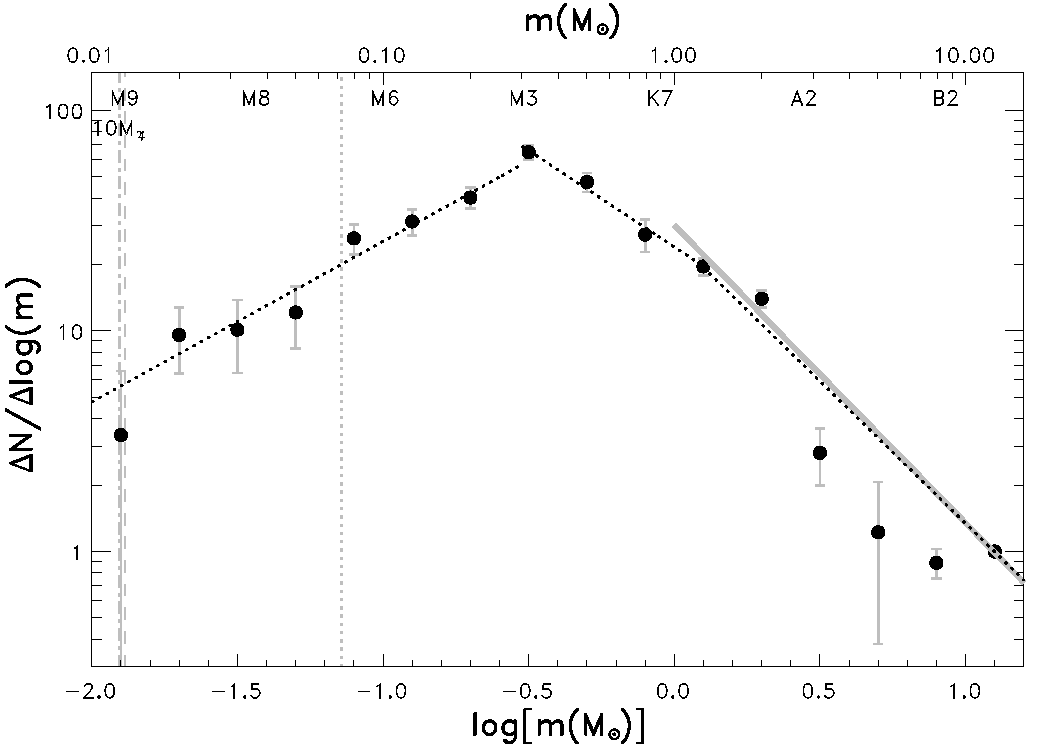
\includegraphics[width=.33\linewidth]{IMF_FOV_0-5deg_spl.pdf}} & 
		\subfloat{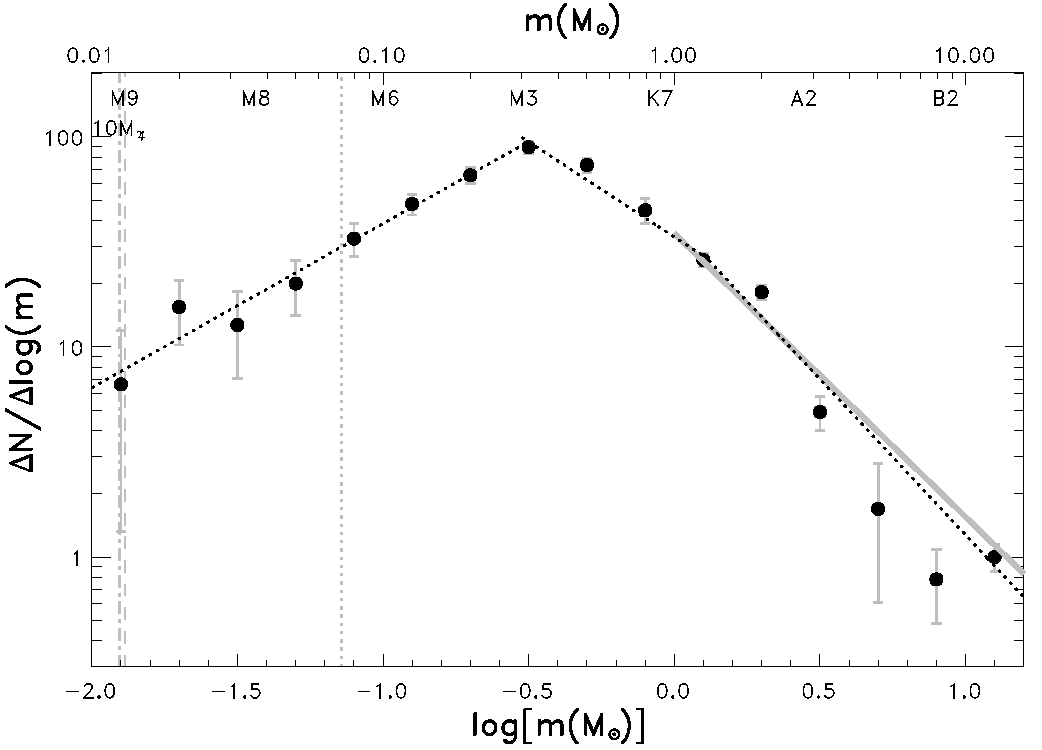
\includegraphics[width=.33\linewidth]{IMF_FOV_0-7deg_spl.pdf}} &
		\subfloat{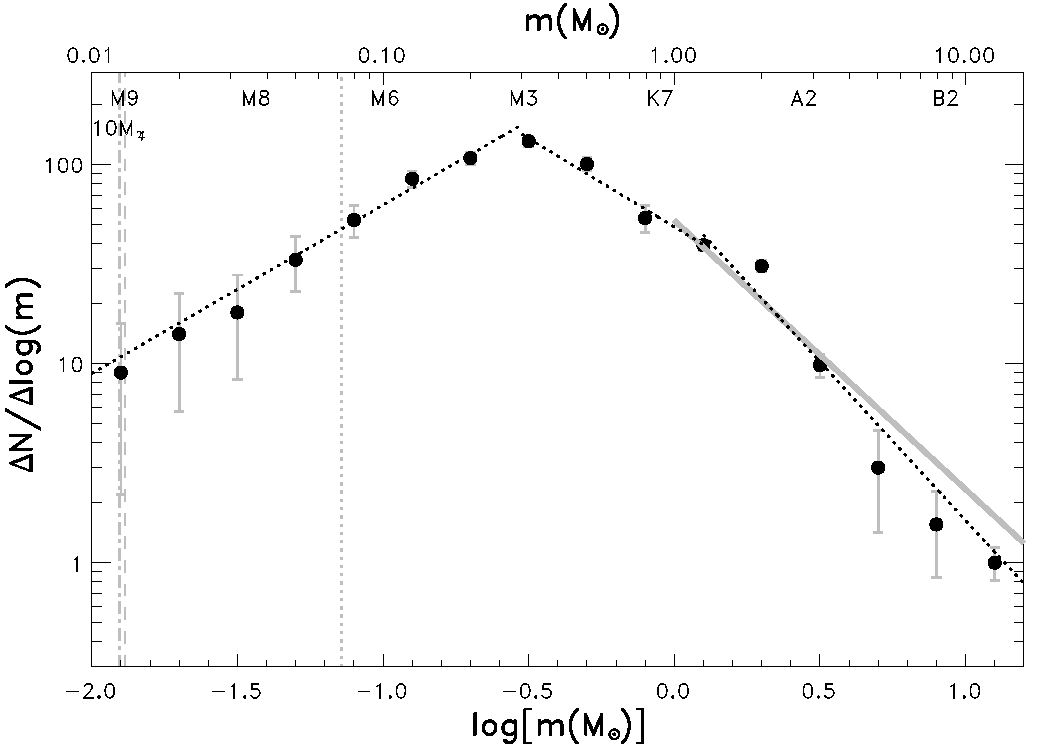
\includegraphics[width=.33\linewidth]{IMF_FOV_1-0deg_spl.pdf}} & \\
		\subfloat{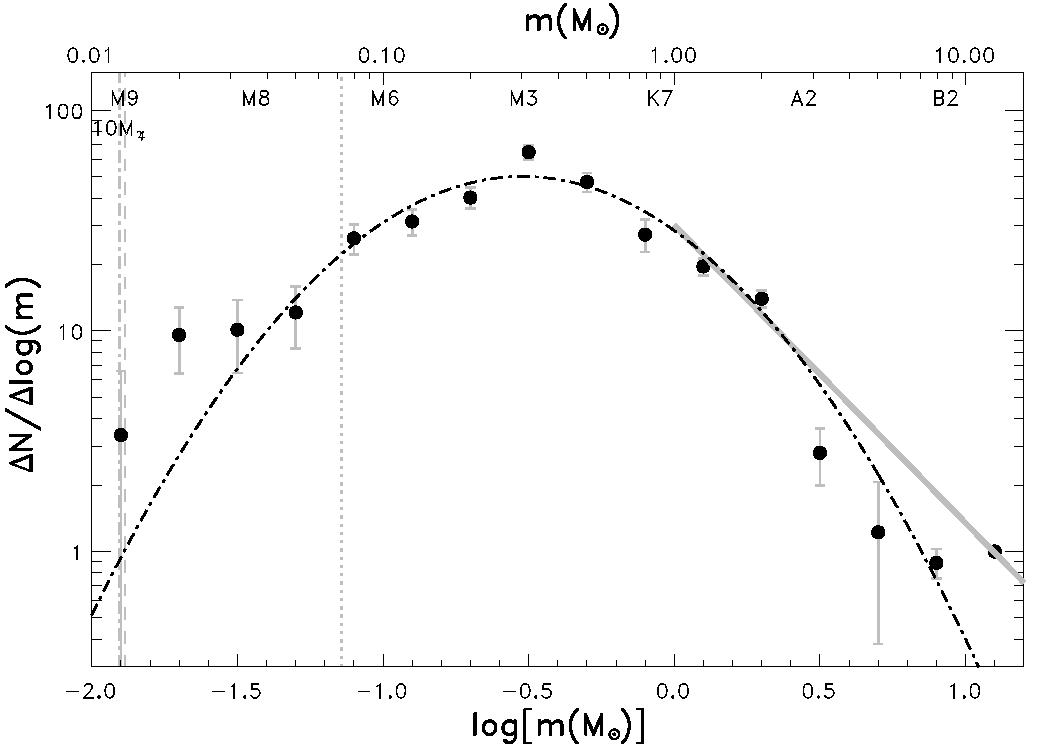
\includegraphics[width=.33\linewidth]{IMF_FOV_0-5deg_lognormal.pdf}} & 
		\subfloat{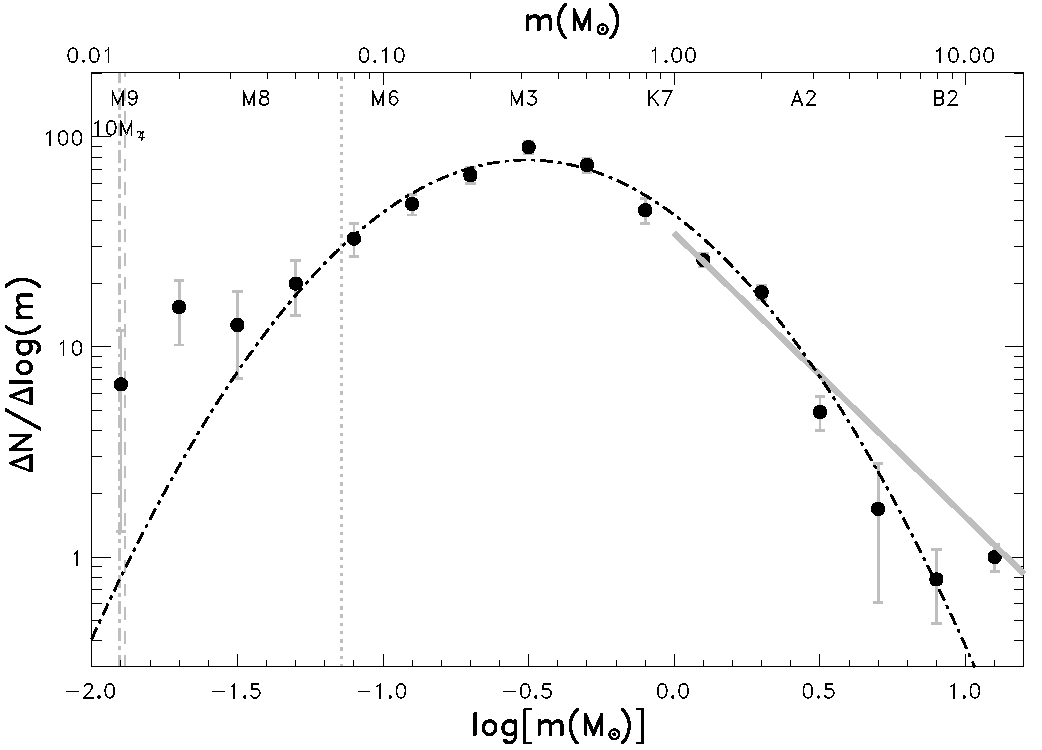
\includegraphics[width=.33\linewidth]{IMF_FOV_0-7deg_lognormal.pdf}} &
		\subfloat{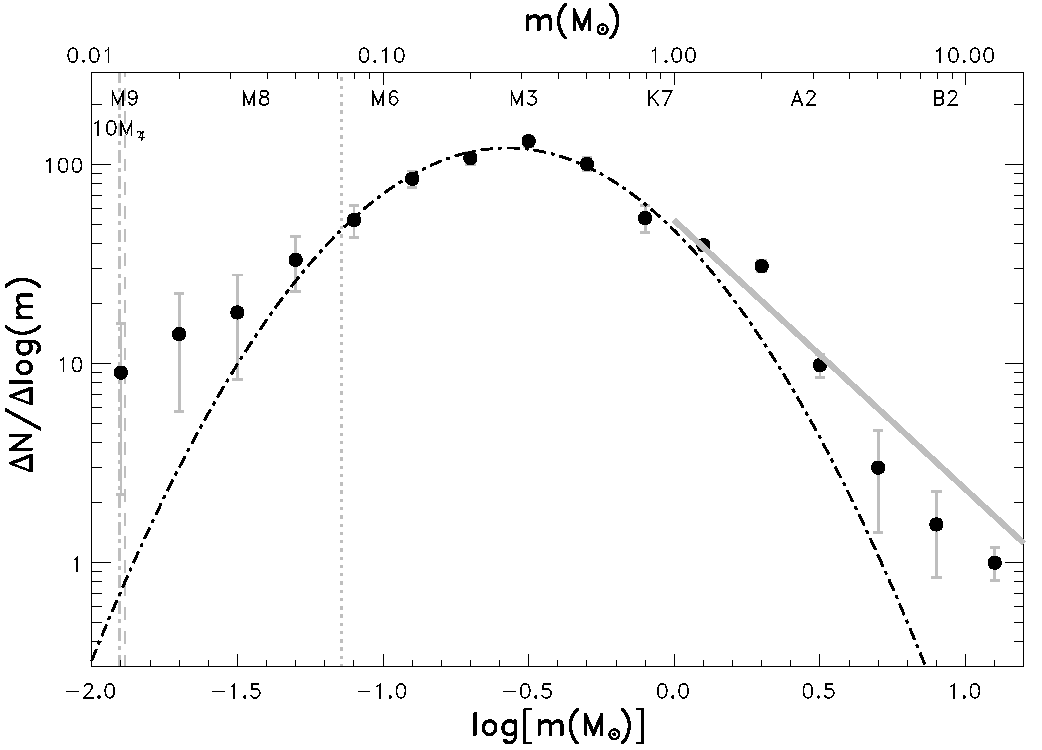
\includegraphics[width=.33\linewidth]{IMF_FOV_1-0deg_lognormal.pdf}} & \\
		\subfloat{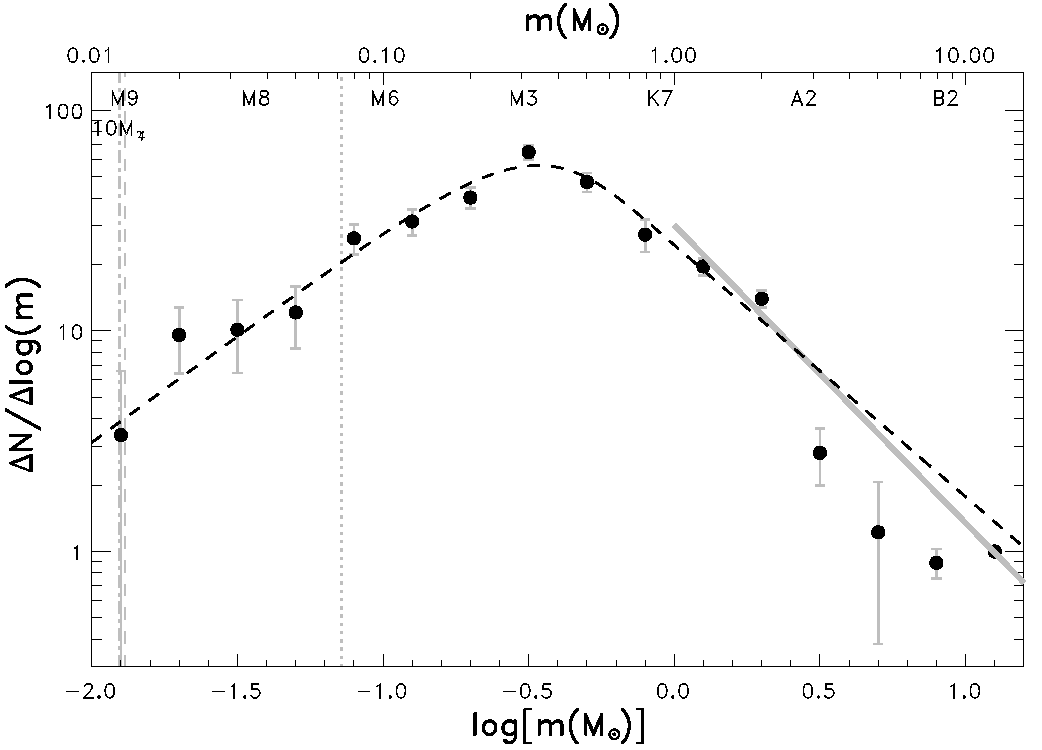
\includegraphics[width=.33\linewidth]{IMF_FOV_0-5deg_tpl.pdf}} & 
		\subfloat{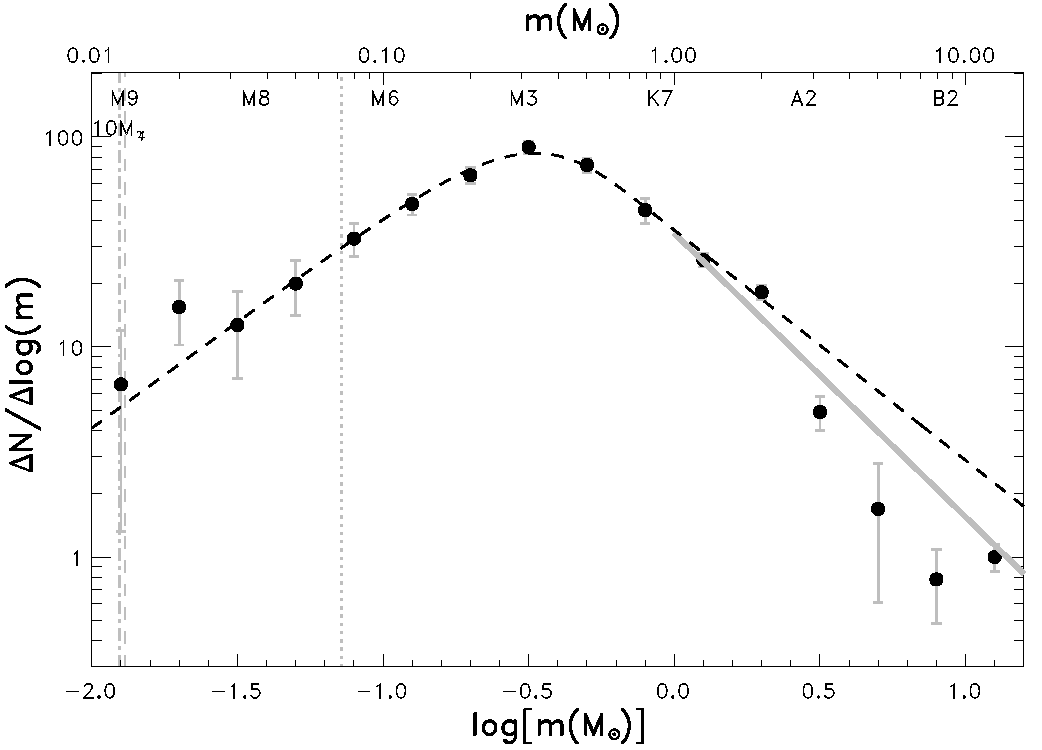
\includegraphics[width=.33\linewidth]{IMF_FOV_0-7deg_tpl.pdf}} &
		\subfloat{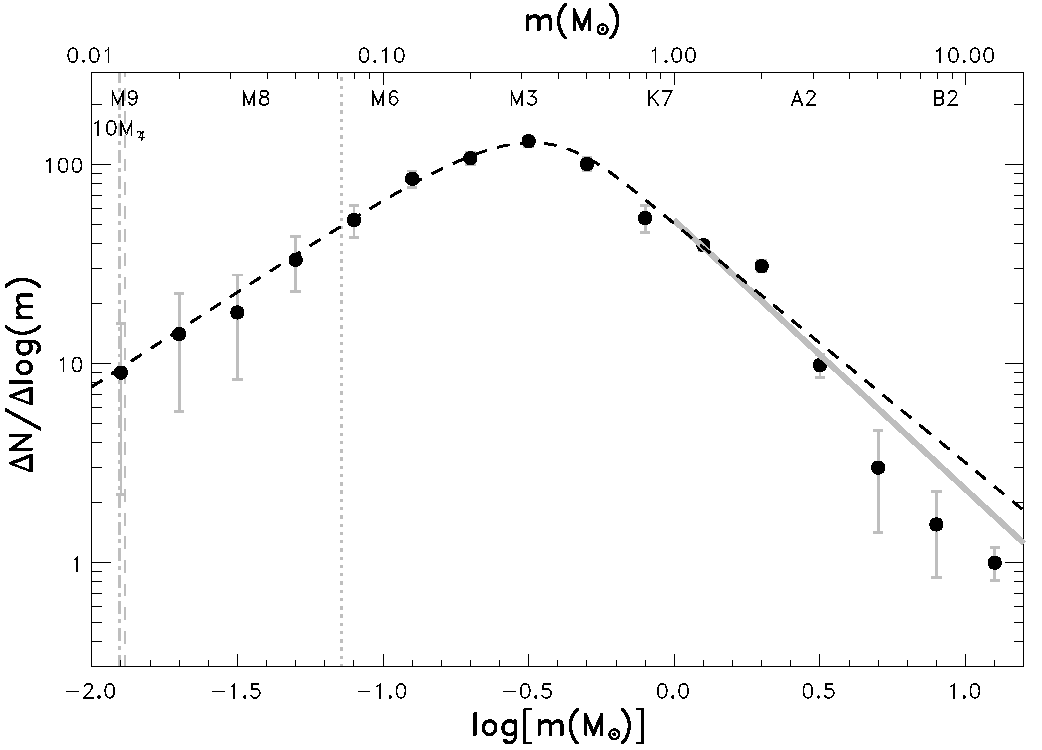
\includegraphics[width=.33\linewidth]{IMF_FOV_1-0deg_tpl.pdf}} 
	\end{tabular}
	\caption[Parameterizations fitted to the 25 Ori system IMFs]{Parameterizations fitted to the 25 Ori system IMFs. Left, central and right panels are the system IMFs considering the areas by \citet[0.5$^\circ$ radius; ][]{Downes2014}, \citet[0.7$^\circ$ radius; ][]{Briceno2018} and \citet[1.0$^\circ$ radius; ][]{Briceno2005,Briceno2007}, respectively. Top, middle and bottom panels show the triple power-law, lognormal and tapered power-law functions, respectively, fitted to the system IMFs. As a reference, the grey line shows the \citet{Salpeter1955} slope ($\Gamma=1.35$). The rest of the symbols and lines are the same as in Figure \ref{fig_IMF:imf}.
	\label{fig_IMF:imf_par}}
\end{figure*}

\begin{table*}
\caption{Parameterizations fitted to the 25 Ori system IMF.}
  \scriptsize
  \label{tab_IMF:imf}
  \setlength{\tabcolsep}{5pt}
  \begin{threeparttable}
 	\begin{tabular}{@{\extracolsep{2pt}}ccccccccc@{}}
 	%\begin{tabular}{p{0.8cm}p{0.3cm}p{0.5cm}p{0.4cm}p{0.4cm}p{0.4cm}p{0.4cm}p{0.1cm}}
 	\hline
 	\hline
		Area           & \multicolumn{2}{c}{Lognormal} & \multicolumn{3}{c}{Triple Power Law}           & \multicolumn{3}{c}{Tapper Power Law} \\
   \cline{2-3}
   \cline{4-6}
   \cline{7-9}
        radius	    & $m_c$        & $\sigma$       & $\Gamma_1$ ($m\le0.3\ M_\odot$) & $\Gamma_2$ ($0.3<m/M_\odot<1.0$)  & $\Gamma_3$ ($m\ge1.0\ M_\odot$)  & $\Gamma$      & $m_p$         & $\beta$      \\
        ($^\circ$)  & $(M_\odot)$  &                &                               &                &               &               & $(M_\odot)$   &             \\
 	\hline
		0.5$^a$       & 0.30$\pm$0.05 & 0.49$\pm$0.07 & -0.73$\pm$0.08 & 0.88$\pm$0.05 & 1.29$\pm$0.10 & 1.14$\pm$0.23 & 0.32$\pm$0.07 & 2.10$\pm$0.18 \\
		0.7$^b$       & 0.31$\pm$0.04 & 0.46$\pm$0.05 & -0.78$\pm$0.06 & 0.91$\pm$0.11 & 1.48$\pm$0.18 & 1.10$\pm$0.09 & 0.31$\pm$0.03 & 2.11$\pm$0.09 \\
		1.0$^c$       & 0.27$\pm$0.02 & 0.42$\pm$0.03 & -0.84$\pm$0.07 & 0.89$\pm$0.07 & 1.59$\pm$0.18 & 1.20$\pm$0.13 & 0.31$\pm$0.05 & 2.15$\pm$0.18 \\
		%0.5$^a$       & 0.30$\pm$0.04 & 0.47$\pm$0.07 & -0.73$\pm$0.12 & 0.87$\pm$0.05 & 1.29$\pm$0.10 & 1.12$\pm$0.24 & 0.32$\pm$0.07 & 2.10$\pm$0.19 \\
		%0.7$^b$       & 0.31$\pm$0.04 & 0.47$\pm$0.06 & -0.72$\pm$0.08 & 0.91$\pm$0.10 & 1.48$\pm$0.18 & 1.10$\pm$0.10 & 0.31$\pm$0.05 & 2.06$\pm$0.14 \\
		%1.0$^c$       & 0.26$\pm$0.02 & 0.44$\pm$0.04 & -0.69$\pm$0.05 & 0.89$\pm$0.07 & 1.59$\pm$0.18 & 1.23$\pm$0.14 & 0.33$\pm$0.07 & 2.04$\pm$0.16 \\
 	\hline
 	\end{tabular}
  \begin{tablenotes}[para,flushleft]
	$^a$By \citet{Downes2014}.\\
	$^b$By \citet{Briceno2005,Briceno2007}.\\
	$^c$By \citet{Briceno2018}.
  \end{tablenotes}
 \end{threeparttable}
\end{table*}

\subsubsubsection{Comparison of the 25 Ori system IMF with Other Studies}
\label{sec_IMF:imf_comparison}
Before comparing the system IMF reported here with that in other clusters, we considered the 25 Ori system IMF obtained by \citet{Downes2014}. They found that the system IMF in the entire survey (3x3 deg$^2$ around the 25 Ori overdensity) is well described by either two power laws with slopes $\Gamma_a=-2.73\pm0.31$ and $\Gamma_b=-0.32\pm0.41$ for the mass ranges $0.02\le m/M_\odot\le0.08$ and $0.08\le m/M_\odot\le0.5$, respectively, or a lognormal function with parameters $m_c=0.21\pm0.02$ and $\sigma=0.36\pm0.03$ for the whole studied mass range. Additionally, for the system IMF of the overdensity (0.5$^\circ$ radius), they obtained $\Gamma_a=-2.97\pm0.02$ and $\Gamma_b=-0.63\pm0.04$, and $m_c=0.22\pm0.02$ and $\sigma=0.42\pm0.05$ in the corresponding mass ranges. These $m_c$ and $\sigma$ values are slightly lower than ours, regardless the considered area, and their slope for substellar masses is quite steeper. Precisely, they reported that 25 Ori may have a lower number of BDs when comparing with the Galactic-disk IMF from \citet{Chabrier2003b}. We stress that they worked with the CDSO catalogue, which is also part of this study. Despite this catalog is complete at $\sim0.03\ M_\odot$, considering the BT-Sett 7 Myr isochrone, they dealt with incompleteness issues related to the width of their locus and to the dispersion of the candidates for masses $m<0.06\ M_\odot$. Thus, most of the mass range where they fitted the substellar slope presents this issue. 
%\textcolor{green}{ESTA PARTE DE LA RESOLUCION DEBE MENCIONARSE EN LA SUBSECCIÓN 3.2.7 DONDE TE DECIA QUE FALTA MENCIONAR COMO MANEJASTE EL PROBLEMA DE LA RESOLUCI´ON}
Additionally, we observed in the DECam images (0.9'' spatial resolution) that an important fraction ($\sim15$ per cent) of the faint detections ($I_c\gtrsim17$) in the entire CDSO catalogue (2.9'' spatial resolution) are unresolved sources. This yields a lost of sources in the CDSO and, hence, in the candidate selection. Therefore, we mainly attribute the differences between both system IMFs to these lost unresolved sources and to the treatment of the mentioned incompleteness as well as to the differences in the procedures for estimating masses (they worked with the H-R diagram and us with the mass-luminosity relation in Section \ref{sec_IMF:mass-luminosity}). In this study, we used our deeper DECam photometry, instead of that from the CDSO, for masses $m<0.08\ M_\odot$. Hence, we presented here an updated version of the 25 Ori system IMF.

In order to contribute to the understanding of the origin of the IMF and its relation with the environment, we compared the parameters of the multi-segmented power-law and lognormal functions fitted to the 25 Ori system IMF with those in Table \ref{tab_IMF:imf_literature}, mainly because those IMFs cover a wide mass range as that presented here, and with other studies of interest to include as well the tapered power-law parametrizations. In these comparisons we assumed similar binarity properties for the different clusters and similar spatial resolutions of the surveys.
%\textcolor{green}{DEBES REESCRIBIR ESTA ULTIMA FRASE. PUEDES ASUMIR IGUALES PROPIEDADES DE BINARIEDAD PERO NO PUEDES ASUMIR LA RESOLUCIÓN DE LOS SURVEYS. LOS SURVEYS TIENEN UNA DADA RESOLUCIÓN. DEBES EXPLICAR LO QUE QUIERES DECIR.}

The best fitted lognormal function to the 25 Ori system IMF are roughly consistent, within the uncertainties, with those obtained in the clusters mentioned in Table \ref{tab_IMF:imf_literature}. The values of $m_c$ goes from 0.25 to 0.36, with the most dispersed values in the oldest associations. $\sigma$ takes values between 0.38 and 0.53, considering only those obtained for masses $<$1 $M_\odot$. Also, these values are consistent with a set of young clusters in \citet{Bayo2011}. Despite we compared the best fitted lognormal function, we stress that this functional form tends to underestimate the number of BDs in 25 Ori. A similar result was reported in $\sigma$ Ori by \citet{PenaRamirez2012}. 
%\textcolor{green}{EXPLICALO MEJOR. NO SE ENTIENDE. UN AJUSTE ES UN AJUSTE. NO PUEDE SUB-ESTIMAR LAS COSAS A LAS QUE SE AJUSTA. QUIZAS EL COMENTARIO SEA SOBRE QUE LAS EM TIENEN MENOR PESO POR SU CANTIDAD?}

From the power-law fit, the slope we obtained for high-intermediate masses is consistent with the \citet{Salpeter1955} slope ($\Gamma=1.35$) and with the most representative slope for $m\ge1\ M_\odot$ from a large sample of stellar associations in \citet{Bastian2010}, which covers a diversity of physical conditions such as age, metallicity and total mass. However, this slope is slightly steeper than those for most clusters in Table \ref{tab_IMF:imf_literature}, nevertheless, it is worth to stress the different break masses considered in those studies. In most of the studies in the table, this slope is fitted for masses down to the peak of the IMFs ($\sim0.3\ M_\odot$), while for the case of 25 Ori, it is better described by a dual power-law with a break mass at 1 $M_\odot$ (see Figure \ref{fig_IMF:imf}). However, if we consider the break mass for high-intermediate masses at $\sim0.5\ M_\odot$, the slope fitted to the 25 Ori system IMF in this range is somewhat shallower than when considering the break mass at 1 $M_\odot$ and is more consistent with the clusters in the table.

The tapered power-law fitted to our system IMF is roughly consistent with that fitted to an extended sample of young clusters (25 Ori not included) by \citet{DeMarchi2010} and \citet{Bastian2010}, which has the parameters $\Gamma=1.1\pm0.2$, $m_p=0.23\pm0.10$ and $\beta=2.4\pm0.4$. The $m_p$ value is slightly higher in our system IMF but the differences are in agreement within the errors.

These comparisons indicate that the 25 Ori system IMF show a similar behaviour to that in a diversity of stellar clusters, which supports the idea that the shape of the IMF is almost insensitive to environmental properties, as predicted by the models from \citet{Bonnell2006} and \citet{Elmegreen2008}.
%\textcolor{green}{CREO QUE NO ES BUENO USAR LA PALABRA "DIVERSITY". ES CONTRADICTORIA PORQUE PARTIMOS DE LA BASE DE QUE HAY POCAS IMF COMPARABLES CON LA NUESTRA. POR LO TANTO LA MUESTRA NO ES TAN DIVERSA. EN TAL SENTIDO CREO QUE LA CONCLUSION RESPECTO A LA INDEPENDENCIA DE LAS CONDICIONES AMBIENTALES DEBE SER MAS CUIDADOSA Y PRECISA MENCIONANDO QUÉ PROPIEDADES TIENEN ESAS POBLACIONES QUE ESTAMOS CONSIDERANDO PARA LLEGAR A ESA CONCLUSIÓN.}

Also, the continuity of the mass distribution across the entire range is an indicative of similarities between planetary mass objects to high-mass stars, which supports the idea of a common physical mechanism for the formation of these objects.
%\textcolor{green}{NO ESTOY DE ACUERDO CON ESTE PARRAFO. LO QUE ANALIZAN RC2001 ES LA EYECCIÓN PREMATURA DE CORES QUE, POR DEFINICIÓN, ES UN MECANISMO DEPENDIENTE DE LA MASA PUES APLICA A LOS OBJETOS MENOS MASIVOS. LAS SIMILARIDADES MENCIONADAS DEBEN SER MEJOR REFERENCIADAS.}

\subsubsection{BD/star ratio}
\label{sec_IMF:BD_star_ratio}

A useful quantity that indicates the efficiency to form stellar and substellar objects is, precisely, the ratio between BDs and stars. We worked with the $R_{ss}$ definition by \citet{Briceno2002}, which considers objects with masses between 0.02 and 10 $M_\odot$ and the BD-star limit at 0.08 $M_\odot$. If we consider radius of $1.1^\circ$ (FOV of our DECam data) and decreasing it by steps of $0.1^\circ$ until having a radius of $0.4^\circ$, $R_{ss}$ takes values between 0.14 and 0.16, which are basically the same within the uncertainties. For the 25 Ori areas of 1.0, 0.7 and 0.5$^\circ$ radius, $R_{ss}$ is $0.14\pm0.03$, $0.15\pm0.02$, $0.15\pm0.02$, respectively. These identical $R_{ss}$ values for different areas indicate that the 25 Ori substellar and stellar population have similar spatial distributions.
% with radius of $1.1^\circ$ and decreasing it by steps of $0.1^\circ$ until having a radius of $0.5^\circ$ take values between 0.20 and 0.14, which slighly increase with the radius. For the 25 Ori area by \citet[0.5$^\circ$ radius; ][]{Downes2014}, \citet[0.7$^\circ$ radius; ][]{Briceno2018} and \citet[1.0$^\circ$ radius; ][]{Briceno2005,Briceno2007}, we obtained $R_{ss}$ values of $0.14\pm0.02$, $0.16\pm0.02$ and $0.18\pm0.03$. The increase of these values when considering larger areas suggests that substellar objects are more dispersed than stellar objects. However, this trend is not very pronounced and the differences in the ratios are in agreement within the uncertainties. A similar gradient for this ratio was obtained by \citet{Andersen2011} in the ONC, which was interpreted as a mass segregated cluster. 

%\vspace*{2ex}
The $R_{ss}$ value representative of 25 Ori is $0.15\pm0.03$ i.e. for each 7 stars in 25 Ori we roughly expect 1 BD. This value is consistent with those found in Taurus \citep{Briceno2002} and Blanco 1 \citep{Moraux2007a}, which are clusters with low stellar densities comparable with that in 25 Ori. Also, this value is consistent, within the uncertainties, with that in other regions with higher stellar densities by orders of two or more such as the Trapezium \citep{Muench2002}, ONC \citep{Kroupa-Bouvier2003}, NGC 6611 \citep{Oliveira2009}, Chamaeleon-I and Lupus-3 \citep{Muzic2015}, IC 348 \citep{Scholz2013} and RCW 38 \citep[as a lower quote; ][]{Muzic2017}. Furthermore, the BD to star ratio we found in 25 Ori is consistent with that on the Galactic plane \citep{Bihain-Scholz2016}. These comparisons supports the idea that the role the environment plays in the formation of substellar and stellar masses is minimum.
%\textcolor{blue}{SE CUIDADOSO AQUI: PUEDES CONCLUIR ESTO SOBRE POBLACIONES DE CIERTO TIPO. LA FRASEE ES MUY GENERAL Y POR LO TANTO SUENA EXAGERADA. YO NO USARIA LA PALABRA NEGLIGIBLE. ES MUY FUERTE.}, keeping similar proportions in clusters with a diversity of environments. A significantly lower ratio is reported in Collinder 69 \citep[$R_{ss}=0.06$; ][]{Bayo2011}, which calls for more studies in this region covering more extended areas. \textcolor{blue}{QUE DICE EL PAPER DE AMELIA SOBRE ESTE VALOR ATIPICO?}

%{\bf volviendo a lo mismo, el BD/S crece un poquito como funcion del radio, lo cual es compartible con la idea de segregar las BD hacia afuera en procesos primordiales. }

%++++++++++++++++++++++++++++++++++++++++++++
\subsubsection{Mass Segregation}
\label{sec_IMF:mass_segregation}

Mass segregation is an interesting phenomenon present in some clusters with different ages \citep[e.g. ][]{Lada-Lada2003}, which opens the question about if it is a primordial property \citep{Bonnell-Davies1998,Bonnell2001} or due to dynamical evolution \citep{Kroupa2001a,Kroupa2001b} of clusters. With the large coverage in mass and area of the system IMF reported here, we can analyse this phenomenon in the 25 Ori population.%an association where no dynamical evolutionary effects are expected \citep{deLaFuenteMarcos-deLaFuenteMarcos2000}.
%its behaviour as a function of the radius, which could contribute to the understanding of this phenomenon.

%In Table \ref{tab:imf} and Figure \ref{fig:imf_par} we observe that the slope fitted to the very low-mass stars and BDs becomes flatter when increasing the radius. Furthermore, the slope for the intermediate and high-mass stars becomes steeper with the radius; a feature also observed in other regions such as NGC 3603 \citep{Stolte2006,Harayama2008}, Arches \citep{Habibi2013} and Westerlund 1 \citep{Brandner2008,Andersen2017}. These systematic features in both sides of the 25 Ori system IMF keep when considering other radius between 0.5 and 1.1$^\circ$ and are evidence of some degree of mass segregation. However, we stress that the changes in the slopes are in agreement within the uncertainties and the slope for the intermediate and high-mass stars is based on small-number statistics. Additionally, it can be due that the increase of substellar objects for larger areas is related to the presence of other young groups in Orion OB1a (see Figure \ref{fig:sky}).

In Table \ref{tab_IMF:imf} and Figure \ref{fig_IMF:imf_par} we observe that the slope for the intermediate and high-mass stars becomes steeper with the radius, which is also obtained for other radius between 0.4 and 1.1$^\circ$ with increases of 0.1$^\circ$. A similar feature of this slope is also observed in other regions such as NGC 3603 \citep{Stolte2006,Harayama2008}, Arches \citep{Habibi2013} and Westerlund 1 \citep{Brandner2008,Andersen2017}, which was interpreted as evidence of some degree of mass segregation. In the case of 25 Ori, this behaviour is not very pronounce and is largely contained within the uncertainties. Therefore, we mostly attribute the change of this slope to the associated errors due to the fits are based on small-number statistics. Additionally, the peak of the system IMF moves towards lower masses with the radius, taking values between 0.35 and 0.26 $M_\odot$ for radius between 0.4 and 1.1$^\circ$. A similar behaviour was observed in the ONC \citep{Hillenbrand2000} and IC 348 \citep{Muench2002}. Nevertheless, we stress that for 25 Ori, the change of the peak is smaller than the bin size of the system IMF (0.2 dex). 

We observe that the slopes fitted to the very low-mass stars and BDs are in agreement, within the uncertainties, for the different 25 Ori radius. This slope keeps constant for the other radius between 0.4 and 1.1$^\circ$ with increments of 0.1$^\circ$, which suggests that the very low-mass stars and BDs do not have any preferential distribution. 

Hence, we do not observed significant differences between the 25 Ori system IMF for different radius, but future analysis, working with the spectroscopically confirmed members resulting from our sample, will help to understand the possible trends in the slope for the high-mass stars and in the peak of the system IMF.
%as discussed by \citet{Muench2002}, in very young clusters the mass segregation mostly affects to the higher mass stars ($m>1\ M_\odot$), which could be the case of 25 Ori.

\subsubsection{Gravitational State of 25 Ori}
As mentioned by \citet{Lada-Lada2003}, most clusters are dissolved before they reach an age of 10 Myr; only less than 10 per cent reach older ages and about 4 per cent survive longer than 100 Myr. 25 Ori is just at this critical point and not conclusive results about its gravitational state have been presented \citep{McGehee2006,Downes2014}. Any cluster, to be gravitationally bound, its escape velocity, $v_{esc}=(2GM/R)^{(1/2)}$, must be larger than its velocity dispersion \citep{Sherry2004}.

Directly counting in the mass distributions shown in Figure \ref{fig_IMF:imf}, we obtained a total mass of $168\pm8$, $236\pm10$ and $355\pm14$ $M_\odot$ contained in 25 Ori inside areas of 0.5, 0.7 and 1.0$^\circ$ radius, respectively. The fraction of these masses contained in BDs is $1.34\pm0.35$, $1.34\pm0.32$ and $1.35\pm0.29$ per cent, respectively. Similar values are obtained for other radius between 0.4 and 1.1$^\circ$, which also indicates, as from the $R_{ss}$ ratio, alike spatial distribution of the substellar and stellar population of 25 Ori.
%When considering other radius between 0.5 and 1.1$^\circ$, there is a gradient of the total mass contained in BDs, which could also suggests a small degree of mass segregation in 25 Ori, as discussed above.

Considering the total mass of 355 $M_\odot$ inside a radius of 1.0$^\circ$, which corresponds to 6.2 pc at a distance of 356 pc, the resultant $v_{esc}$ is 0.7 km/s. A similar $v_{esc}$ is obtained if considering the total mass inside the 0.7 or 0.5$^\circ$ radius. This $v_{esc}$ is about 3 times smaller than the velocity dispersion of 2 km/s in 25 Ori \citep{Briceno2007}, which indicates that 25 Ori is an unbound association. 
%\textcolor{green}{CREO QUE ESTA FRASE NO ES NECESARIA. LA DIFERENCIA EN LAS VELOCIDADES ES TAN GRANDE QUE NO ES NECESARIO ENFATIZARLO MAS}. 
We estimated that to be a gravitationally bound cluster, 25 Ori should have about 10 times more mass than that estimated here, which implies an unrealistic number of more than 6000 members, or to have a significantly smaller velocity dispersion.

\subsection{Summary and Conclusions}
\label{sec_IMF:conclusions}

% About the sample and contamination
By combining optical and NIR photometry from DECam, CDSO, UCAC4 and $Hipparcos$, and VISTA and 2MASS, respectively, we selected a sample of 1687 photometric member candidates in an area of 1.1$^\circ$ radius around the 25 Ori overdensity on the basis of their position in colour-magnitude and colour-colour diagrams. This sample covers an $I_c$ range between 5.08 and 23.30 mag, which corresponds to a mass range from $0.011$ to 13.1 $M_\odot$. The completeness of the sample is at 0.012 $M_\odot$, which is just beyond the Deuterium burning limit (0.013 $M_\odot$), and also  includes the most massive stars in 25 Ori. We estimated a contamination of 20 per cent for the LMS candidates, but it increases for the intermediate-mass candidates due to giant and subgiant stars and for BD candidates due to extragalactic sources.

Additionally, we discussed and/or considered, in the context of 25 Ori, the following uncertainties and biases to be taken into account when determining the mass distribution: spatial completeness, photometric sensitivity, IR excesses, chromospheric activity, unresolved binaries and missed members.

% system IMF
%With this sample of photometric member candidates we constructed their $M_{I_c}$ and mass distributions, which were corrected by the distributions of the contaminants in the control field. In the resultant distributions we replaced the range mostly affected by giant and subgiant stars ($\sim1-5$ mag or $\sim$0.9 and 3 $M_\odot$) by the distributions of our member candidates filtered by their BJ18 distances. This way we constructed the LFs and system IMFs for the different areas estimated for 25 Ori (see Figures \ref{fig:LF} and \ref{fig:imf}). This 25 Ori system IMF is complete down to 12 $M_{Jup}$ to 13.1 $M_\odot$ (corresponding to the 25 Ori star) and is one of the few system IMFs covering the whole mass range of a stellar group \citep[e.g. the $\sigma$ Ori system IMF by ][]{PenaRamirez2012}. 
With the sample of member candidates we constructed the system IMF of 25 Ori for different areas, which is complete down to 12 $M_{Jup}$ to 13.1 $M_\odot$ and is one of the few system IMFs covering the whole mass range of a stellar cluster \citep[e.g. the $\sigma$ Ori system IMF by ][]{PenaRamirez2012}. We parametrized the resultant system IMF using a triple power-law, a lognormal and a tapered power-law function to compare it with other studies. We observed that a lognormal function well-fitted to the peak of the mass distribution underestimates the BD population of 25 Ori.

% Comparison of the system IMF and its implications
We observed some differences in the BD regime when comparing with the system IMF of 25 Ori obtained by \citet{Downes2014}, which can be mainly explained by issues related to the completeness of the CDSO in this mass range. Thus, we discard a low number of BDs in 25 Ori.

In comparison with other clusters having different physical properties, no significant differences were found, which suggest that the conversion of gas into stars and BDs has minimum influence by the environmental properties, as predicted by models \citep[e.g. ][]{Bonnell2006,Elmegreen2008}. Also, the continuity of the system IMF support the scenario of a formation process that extends from planetary mass objects to high-mass stars.
%\textcolor{green}{VER MIS COMENTARIOS ANTERIORES SOBRE LAS CONCLUSIONES. }

% BD/star ratio
We estimated the substellar to stellar ratio of 25 Ori, which has a representative value of $0.15\pm0.03$. This ratio is consistent with that in other regions with low densities, comparable to that in 25 Ori, and others with higher densities as the ONC and RCW 38, which is an indicative that the formation of BDs and stars occurs in a similar way in different environments.
%\textcolor{green}{NUEVAMENTE VER MIS COMENTARIOS ANTERIORES. ADEMAS, RECUERDA QUE NO SOMOS LOS PRIMEROS EN DECIR ESTO Y POR LO TANTO DEBES SUMAR REFERENCIAS. SOMOS LOS PRIMEROS EN DAR UNA IMF COMPLETA PARA 25 ORI.}

% Mass segregation
There are not clear variations of the 25 Ori system IMF with the radius, which indicates that the spatial distributions of the substellar and stellar objects are indistinguishable. However, an analysis of a sample of spectroscopically confirmed members complete in area and mass is required for a study of the mass segregation.
%The possible gradient of the slopes with the radius in both sides of the system IMF is an indicative of some degree of mass segregation in 25 Ori, which, due to its youth, could be interpreted as a primordial property during the cluster formation \citep{Reipurth-Clarke2001}. This effect is also observed in the gradient of the BDs to stars ratio throughout the cluster as well as, in an equivalent way, in the change of the fraction of the total mass contained in BDs as a function of the radius. However, this possible mass segregation is not very pronounced and can be contained within the uncertainties.
%\textcolor{green}{NUEVAMENTE, NO ES CONCLUYENTE LA SEGREGACIÓN Y NO ES PROBLEMA QUE NO LO SEA. HAY QUE BUSCAR UNA MANERA MAS APROPIADA DE DECIR LO QUE ENCONTRAMOS Y PORQUE NO PODEMOS SER CONCLUYENTES.}

% Bound or not
Comparing the escape velocity estimated for 25 Ori and its velocity dispersion, we found that 25 Ori is an unbound association. In fact, 25 Ori should have about 10 times more mass or a significantly smaller velocity dispersion to be considered as a gravitationally bound cluster.

% Ongoing work
The system IMF of 25 Ori we present in this work was constructed with photometric member candidates. To determine the membership of each candidate it is necessary a follow up spectroscopy. Thus, we could determine the distribution of the masses of the confirmed members. This kind of study requires the use of several multi-fiber spectrographs to have full coverage of the brightness range and spatial distribution. In this direction, we have an ongoing spectroscopic survey about 85 per cent complete, which will be part of future works. 

% APPENDICES

\subsection{Appendix: Calibration of the DECam photometry}
\label{sec_app_IMF:DECam_calibration}
To calibrate our DECam photometry we first added the zero point of 25.18 mag from the image headers to the instrumental magnitudes. Then, we compared these instrumental magnitudes with the $i$ magnitudes in the DECam system obtained using the $i$ and $z$-band photometry from SDSS according to Transformation \ref{eq_IMF:DECam_instrumental}\footnote{\url{http://www.ctio.noao.edu/noao/content/Photometric-Standard-Stars-0\#transformations}}.

\begin{equation} \label{eq_IMF:DECam_instrumental}
	i_{DECam}    = i + 0.014 - 0.214*(i-z) - 0.096*(i-z)^2
\end{equation}

where $i_{DECam}$ are in the DECam system and $i$ and $z$ magnitudes are in the SDSS system.

The comparison was done for sources having colours $i-z<0.8$ mag (valid range of the transformation), considering sources not having a high probability of being variable stars according to the CIDA Variability Survey of Orion \citep[][]{Briceno2005,Mateu2012,Briceno2018} and for sources having $i$ and $z$-band photometric errors lesser than 0.05 mag. The mean value of the resultant residuals is 0.637 mag. Thus, we added this value to our DECam photometry to calibrate it. In Figure \ref{fig_IMF:DECam_instrumental} we show the residual between our calibrated photometry and that in the DECam system using the SDSS catalogue. The typical residuals are -0.001 mag with a RMS of 0.038 mag.
%a 0.65 mag zero-point offset with respect to the Sloan Digital Sky Survey (SDSS) Data Release 9 (DR9) \citep{Ahn2012}. This offset was obtained considering roughly 25000 stars from the SDSS, with $i$-band magnitudes between 16.5 and 22.0 and with typical photometric uncertainties of 0.04 mag, which do not have high probability of being variable stars according to the CIDA Variability Survey of Orion \citep[CVSO; ][]{Briceno2005,Mateu2012,Briceno2018}. The detectors of the DECam array having SDSS counterparts lie mainly towards the south of the array, with a few of them (about 6) in the north, representing roughly a half of the whole area covered by the DECam observations and with a typical standard deviation $\sigma$ of the residuals equal to 0.1 mag. We checked that the photometric solutions of these detectors are essentially the same, which allowed us to calibrate confidently those detectors without SDSS counterparts.

\begin{figure}
	\begin{minipage}{0.60\textwidth}
		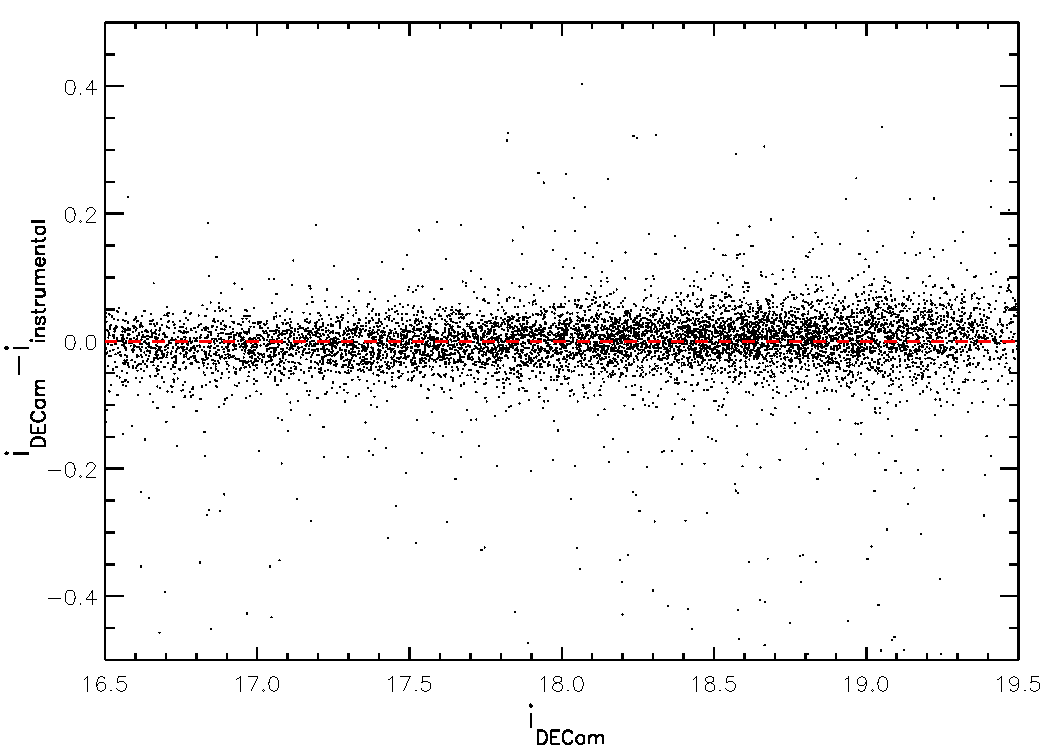
\includegraphics[width=1.00\textwidth]{i_DECam-i_instrumental_vs_i_DECam.pdf}
	\end{minipage} \hfill
	\begin{minipage}{0.35\textwidth}
		\caption[Calibration of the DECam photometry.]{Residual between our calibrated photometry from DECam and the $i$-band photometry in the DECam system obtained using the SDSS catalogue.}
		\label{fig_IMF:DECam_instrumental}
	\end{minipage}
\end{figure}

\subsection{Appendix: Transformation of the UCAC4 and DECam photometry to $I_c$ Magnitudes}
\label{sec_app_IMF:photometry_transformation}

We used transformations from \citet{Jordi2006} and empirical relations obtained directly from our data to convert the $i$-band magnitudes from the UCAC4 and DECam catalogues to the $I_c$-band magnitudes.
%The transformations relate the SDSS and Cousins photometric systems, so we checked that the UCAC4 photometry are in the SDSS system and we transformed our DECam data to the SDSS system.

\subsubsection{UCAC4 Data}
As the transformations from \citet{Jordi2006} relate the SDSS and Cousins photometric systems, we first checked that the UCAC4 photometry are in the SDSS system.

The $r$ and $i$-band photometry in UCAC4 came from the AAVSO \footnote{\url{https://www.aavso.org}} Photometric All-Sky Survey \citep[][]{Henden2016}. These data were taken using the $r'$ and $i'$-band filters from SDSS, whose magnitudes are on the AB system and are close to the $r$ and $i$ magnitudes of SDSS\footnote{\url{http://www.sdss3.org/dr8/algorithms/fluxcal.php\#SDSStoAB}}. In Figure \ref{fig_IMF:SDSS_UCAC4} we show the residuals between the $r$ and $i$ magnitudes from SDSS and UCAC4 as a function of the SDSS magnitudes. We did not consider the sources having $>90\%$ probability of being variables according to the CVSO and only worked with sources having photometric errors lesser than 0.05 mag. In average, these residuals are basically zero for sources brighter than the SDSS saturation limit ($\sim$14 mag), which indicates that the $r$ and $i$-band photometries from UCAC4 can be consider to be in the SDSS photometric system.

\begin{figure*}
	\centering
	\begin{tabular}{cc}
		\subfloat{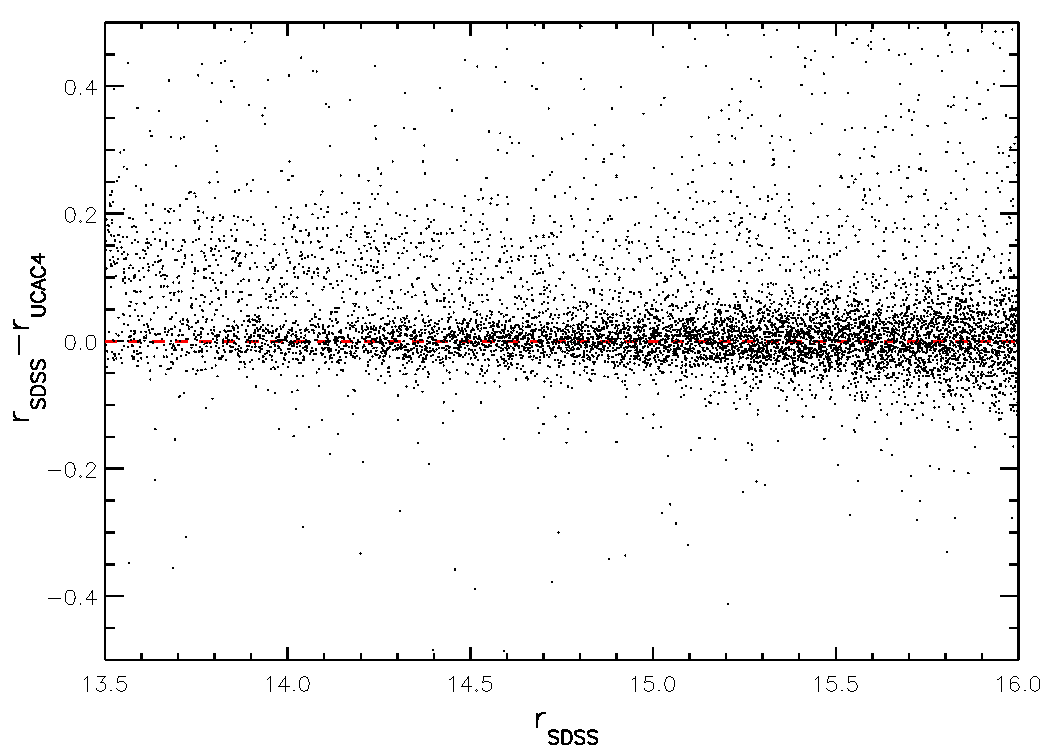
\includegraphics[width=.50\linewidth]{r_SDSS_vs_r_SDSS-r_UCAC4.pdf}} & 
		\subfloat{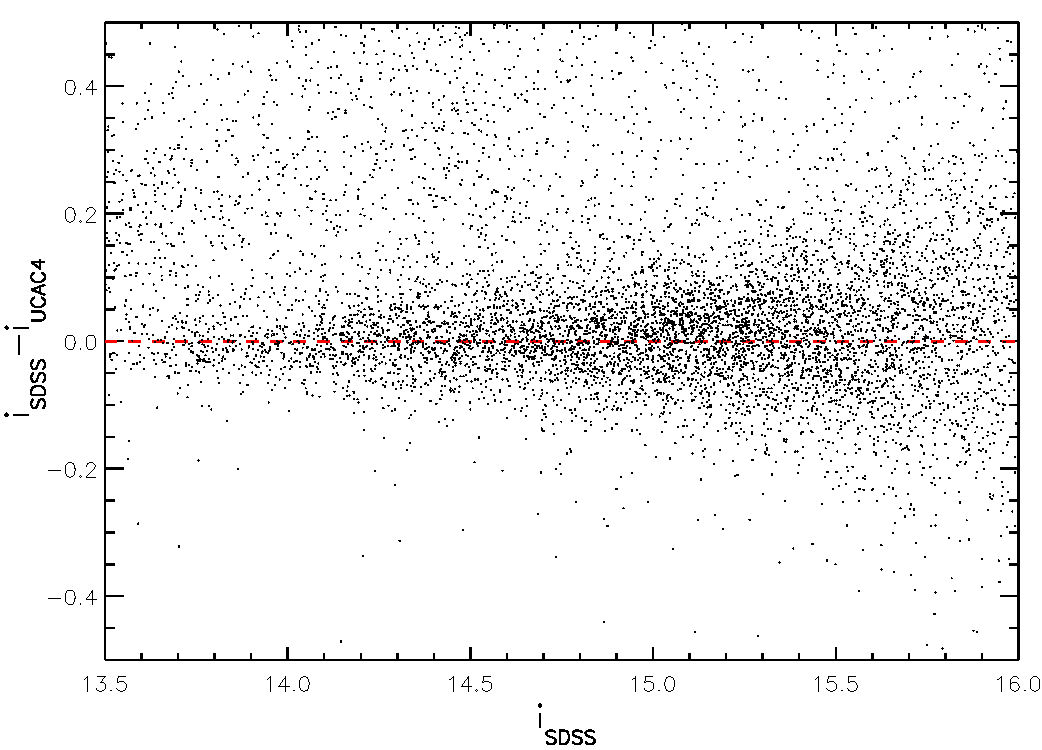
\includegraphics[width=.50\linewidth]{i_SDSS_vs_i_SDSS-i_UCAC4.pdf}} 
	\end{tabular}
	\caption[UCAC4 photometry in the SDSS system.]{Residual between the SDSS and UCAC4 photometries as a function of the SDSS magnitudes in the $r$ and $i$-bands (left and right panels, respectively).}
	\label{fig_IMF:SDSS_UCAC4}
\end{figure*}

Thus, we worked with the following transformations from \citet{Jordi2006}, which use the $r$ and $i$-band magnitudes from SDSS:

\begin{equation} \label{eq_IMF:UCAC_1}
	%R_c-r = (-0.153 \pm 0.003)*(r-i) - (0.117 \pm 0.003)
	R_c-r = -0.153*(r-i) - 0.117
\end{equation}
\begin{equation} \label{eq_IMF:UCAC_2}
	%R_c-I_c = (0.930 \pm 0.005)*(r-i) + (0.259 \pm 0.002)
	R_c-I_c = 0.930*(r-i) + 0.259
\end{equation}

Subtracting Transformation \ref{eq_IMF:UCAC_2} from Transformation \ref{eq_IMF:UCAC_1}:

\begin{equation} \label{eq_IMF:UCAC_3}
	I_c-r = -1.083*(r-i) -0.376
\end{equation}

We used Transformation \ref{eq_IMF:UCAC_3} to obtain the $I_c$ magnitudes considering the $r$ and $i$-band photometry from UCAC4. We compared the resultant $I_c$ magnitudes with those from the CDSO, which are already in the Cousin system. In the left panel of Figure \ref{fig_IMF:trasformation_UCAC4} we show the residual between the $I_c$ magnitudes from the CDSO and UCAC4, where we can see that the peak of the residual distribution is somewhat deviated from zero. Therefore, we did slight modifications to the coefficients of Transformation \ref{eq_IMF:UCAC_3} to have average residuals closer to zero. The resulting transformation is:

\begin{equation} \label{eq_IMF:UCAC_4}
	I_c-r = -1.323*(r-i) -0.353
\end{equation}

In the right panel of Figure \ref{fig_IMF:trasformation_UCAC4} we show the $I_c$ residuals between the CDSO and UCAC4 photometries after applying Transformation \ref{eq_IMF:UCAC_4} to the UCAC4 data. The peak of the $I_c$ residual histograms are essentially zero, with a RMS of 0.07 mag for all the sources within the CDSO saturation limit and the UCAC4 completeness limit (13-14.75 mag).

\begin{figure*}
	\centering
	\begin{tabular}{cc}
		\subfloat{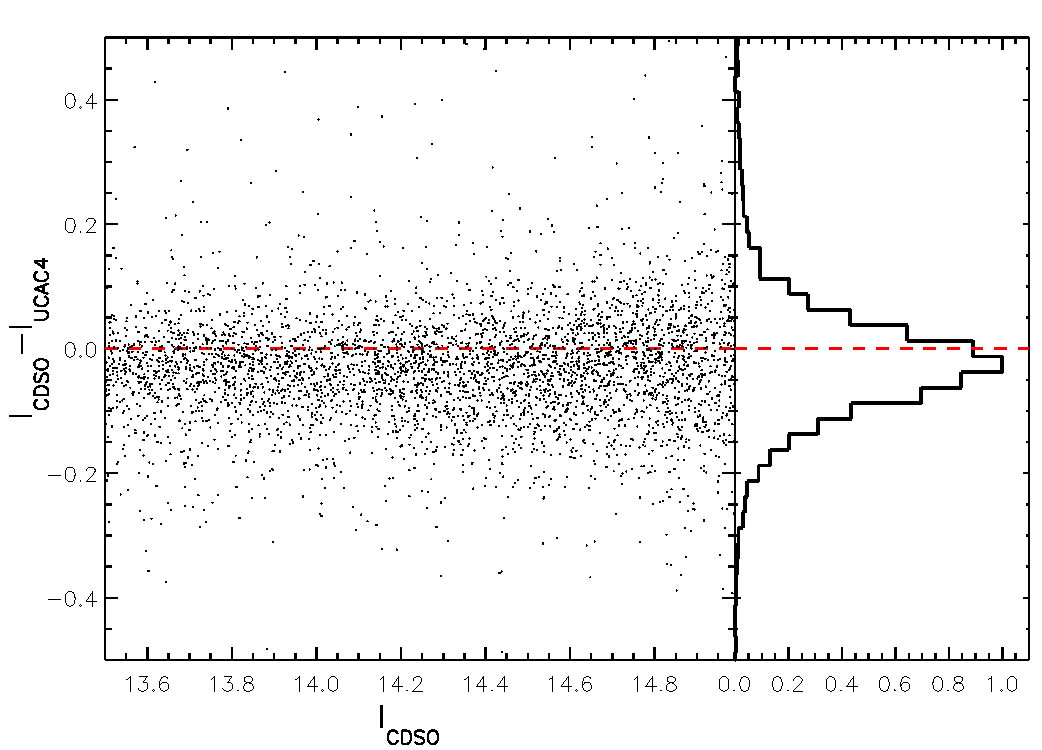
\includegraphics[width=.50\linewidth]{transformation_UCAC4_Jordi2006.pdf}} & 
		\subfloat{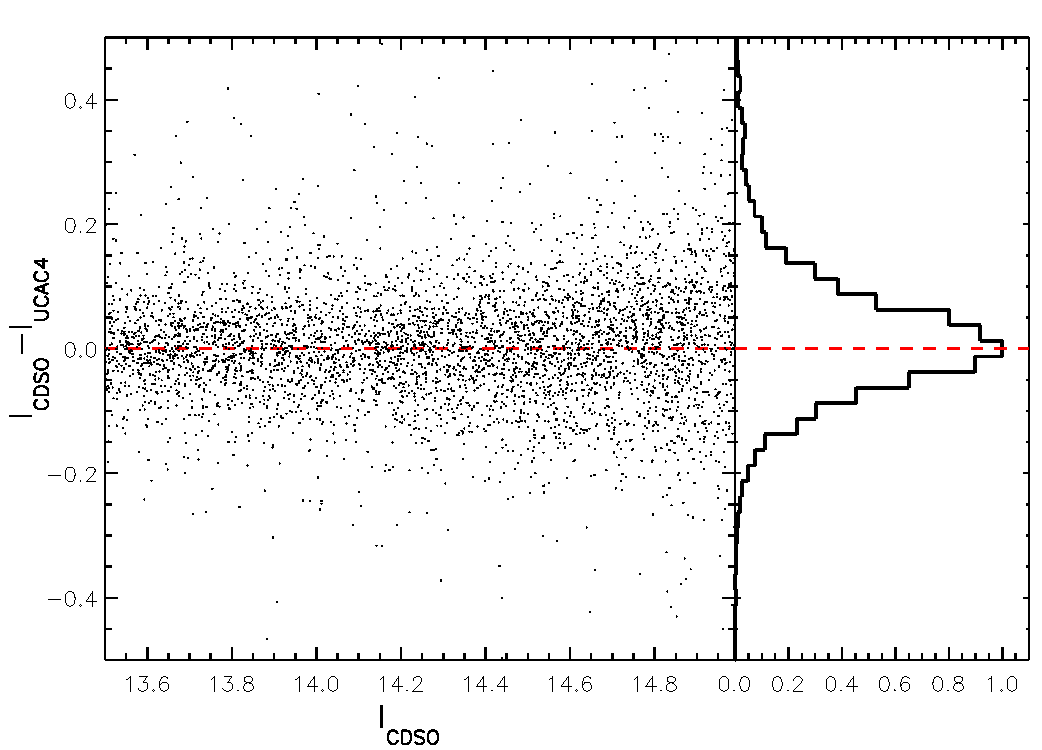
\includegraphics[width=.50\linewidth]{transformation_UCAC4_Jordi2006modified.pdf}} 
	\end{tabular}
	\caption[Transformation of the UCAC4 photometry to the Cousins system.]{$I_c$-residuals between the CDSO and UCAC4 after applying Transformation \ref{eq_IMF:UCAC_3} \citep[left panel; ][]{Jordi2006} and Transformation \ref{eq_IMF:UCAC_4} (right panel), which is a slight modification of Transformation \ref{eq_IMF:UCAC_3}.}
	\label{fig_IMF:trasformation_UCAC4}
\end{figure*}

\subsubsection{DECam Data}
The $i$ filter used in our DECam observations is similar to the $i$ filter from SDSS (NOAO Data Handbook\footnote{\url{http://ast.noao.edu/sites/default/files/NOAO\_DHB\_v2.2.pdf}}). However, there is a colour dependence to transform the DECam data to the SDSS system. As we only have DECam photometry taken with the $i$ filter, in addition to this data we worked with the $Z$-band photometry from VISTA. This way, we will transform the DECam photometry only for the sources with VISTA counterpart, which is not an issue because for the selection of member candidates we used both catalogues. The $Z$-band photometry from VISTA is in the Vega system and to convert it to $z'$-band magnitudes in the AB system it is necessary to add the zero-point of 0.58 mag \citep{Pickles2010}. These $z'$-band magnitudes are not exactly the same as the $z$-band magnitudes in the SDSS system, there is a small shift of 0.02 mag which should be subtracted\footnote{\url{http://www.sdss3.org/dr8/algorithms/fluxcal.php\#SDSStoAB}}. Therefore, we added 0.56 mag to the $Z$-band photometry from VISTA to obtain the $z$-band magnitudes in the SDSS system. In Figure \ref{fig_IMF:trasformation_VISTA} we show the residuals between the $z$ magnitudes directly from SDSS and from VISTA after the addition of the offset. We removed the sources with $>90\%$ probability of being variable according to the CVSO catalogue and we only considered sources with errors lesser than 0.05 mag. The average of the resultant residuals is -0.008 mag with a RMS of 0.04 mag.

\begin{figure}
	\begin{minipage}{0.60\textwidth}
		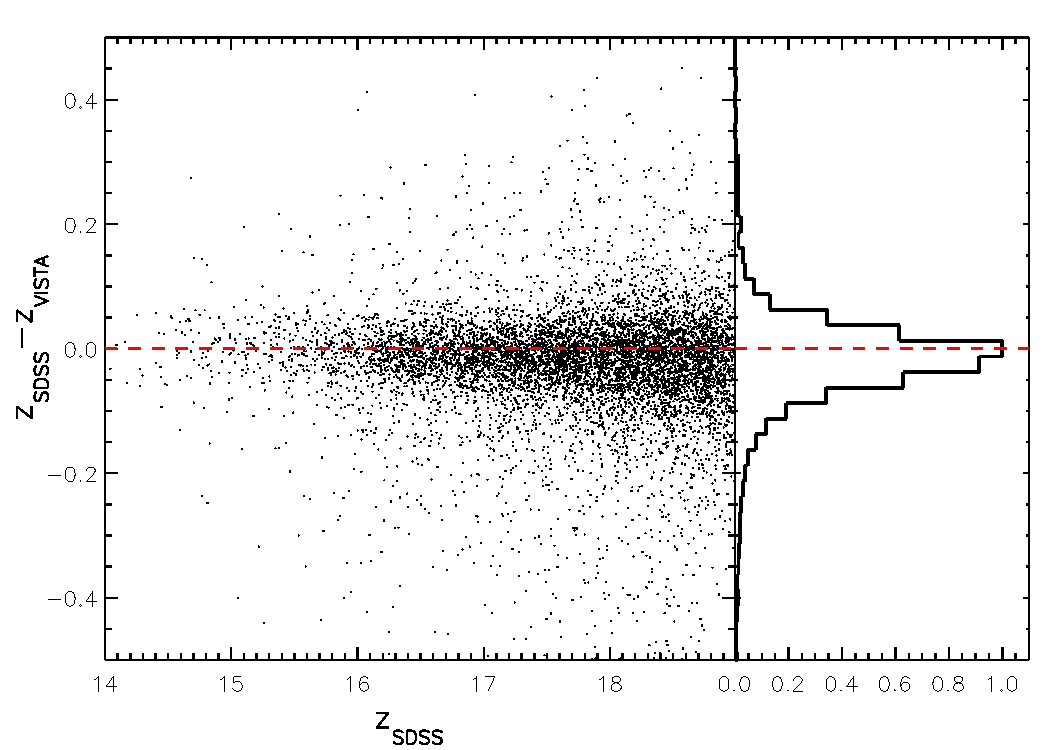
\includegraphics[width=1.00\textwidth]{transformation_VISTA_PD2010.pdf}
	\end{minipage} \hfill
	\begin{minipage}{0.35\textwidth}
		\caption[$Z$ magnidutes from VISTA in the SDSS system.]{Residuals between the $z$ magnitudes in the SDSS system directly from the SDSS catalogue and from VISTA.}
		\label{fig_IMF:trasformation_VISTA}
	\end{minipage}
\end{figure}

In left panel of Figure \ref{fig_IMF:trasformation_DECam_SDSS} we show the colour dependence of the residuals between our calibrated DECam data and those from SDSS as a function of the $i-z$ colour combining the calibrated photometry from DECam and the photometry from VISTA converted to the SDSS system. The second order function that best fits the residuals is:

\begin{equation} \label{eq_IMF:DECam_SDSS}
	i-i_{DECam} = -0.008+ 0.194*(i_{DECam}-z)+ 0.381*(i_{DECam}-z)^2
\end{equation}

where $i_{DECam}$ are in the DECam system and $i$ and $z$ in the SDSS system.

We used Transformation \ref{eq_IMF:DECam_SDSS} to convert our calibrated DECam photometry to the SDSS system. In right panel of Figure \ref{fig_IMF:trasformation_DECam_SDSS} we show the residuals between the $i$-band magnitudes in the SDSS system obtained directly from SDSS and from our calibrated DECam data. The average of the residuals is 0.002 mag with a RMS of 0.04 mag.

\begin{figure*}
	\centering
	\begin{tabular}{cc}
		\subfloat{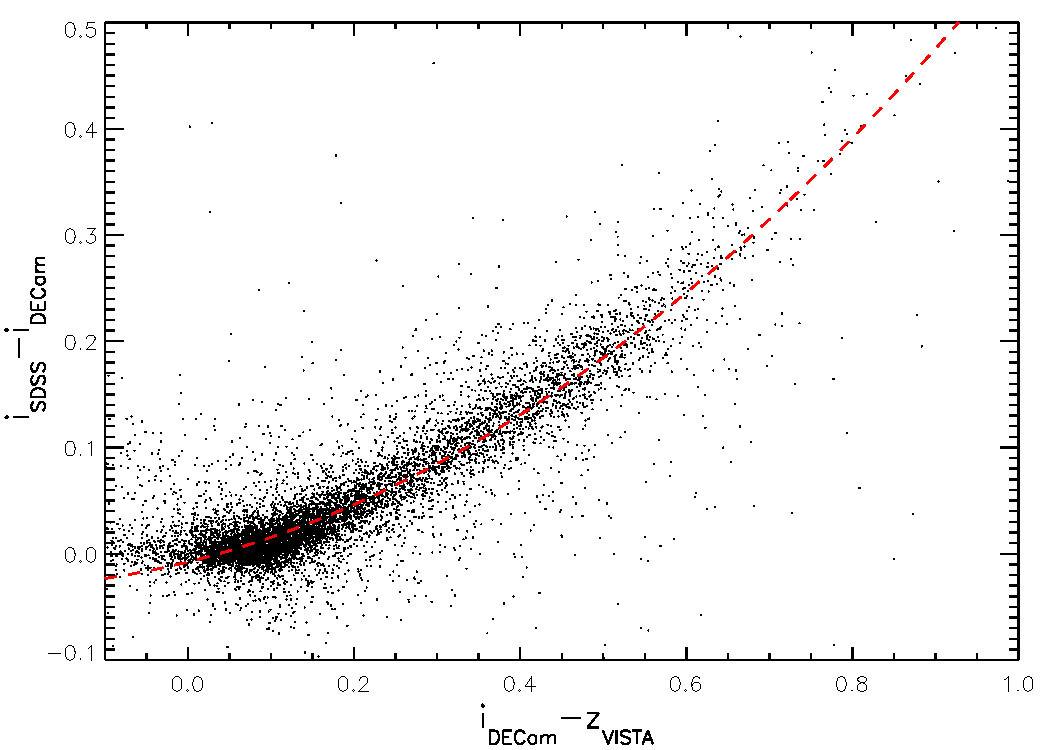
\includegraphics[width=.50\linewidth]{i_SDSS-i_DECam_vs_i_DECam-z_SDSS.pdf}} & 
		\subfloat{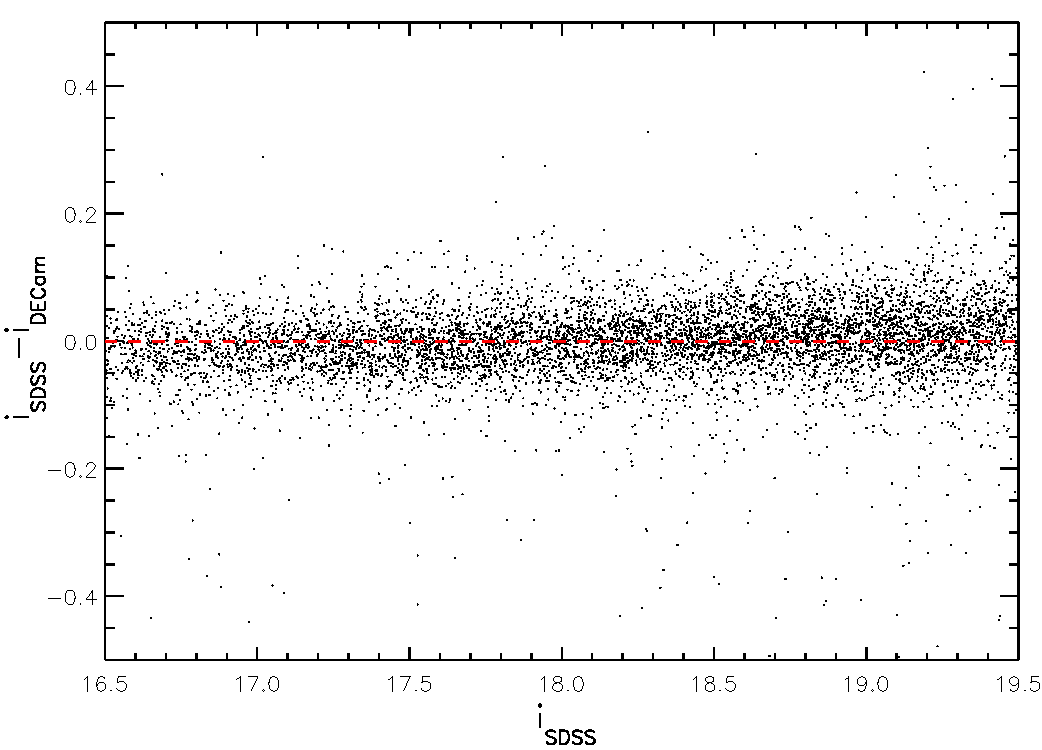
\includegraphics[width=.50\linewidth]{i_SDSS-i_SDSS_DECam_vs_i_SDSS.pdf}} 
	\end{tabular}
	\caption[Transformation of the DECam photometry to the SDSS system.]{{\bf Left panel:} Residuals between the $i$ magnitudes from the SDSS catalogue and from our calibrated DECam data as a function of the $i-z$ colour from DECam and VISTA data in the SDSS system. The red dashed line indicate the second order function fitted to the residuals. {\bf Right panel:} Residuals between the $i$-band photometries in the SDSS system directly from SDSS and from DECam after applying Transformation \ref{eq_IMF:DECam_SDSS}.}
	\label{fig_IMF:trasformation_DECam_SDSS}
\end{figure*}

Finally, once we have both the $i$-band photometry from DECam and the $Z$-band photometry from VISTA in the SDSS system, we converted them to $I_c$ magnitudes in the Cousins system. In left panel of Figure \ref{fig_IMF:trasformation_DECam_CDSO} we show the $i-z$ dependence of the residual between the $I_c$ magnitudes from the CDSO survey and our DECam data in the SDSS system. The second order function fitted to the residual is:

\begin{equation} \label{eq_IMF:DECam_CDSO}
	I_c-i = -0.406-0.446*(i-z)-0.154*(i-z)^2
\end{equation}

where $I_c$ is in the Cousins system and $i$ and $z$ the SDSS system.

We used Transformation \ref{eq_IMF:DECam_CDSO} to obtained the $I_c$ magnitudes from our DECam and VISTA photometries in the SDSS system. In right panel of Figure \ref{fig_IMF:trasformation_DECam_CDSO} we show the residuals between the $I_c$ magnitudes from the CDSO and those obtained from our DECam data. We did not consider neither the sources having $>90\%$ probability of being variable stars in the CVSO catalogue nor the sources with errors larger than 0.05 mag. The resultant residuals have an average of -0.001 mag with a RMS of 0.04 mag.

\begin{figure*}
	\centering
	\begin{tabular}{cc}
		\subfloat{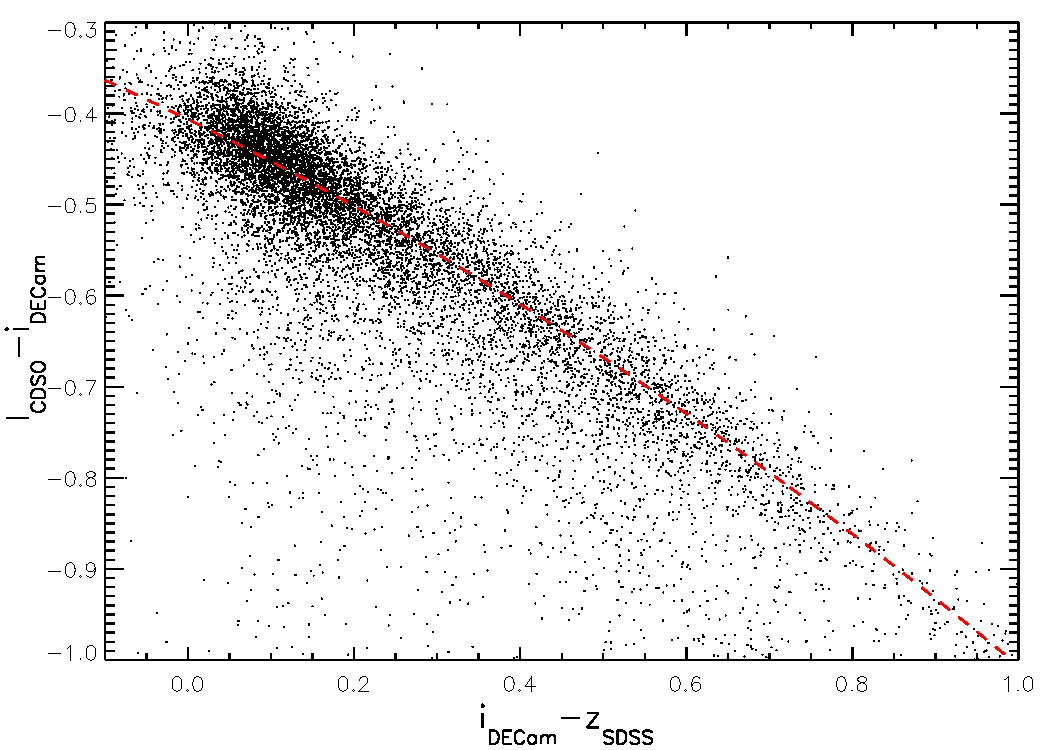
\includegraphics[width=.50\linewidth]{I_CDSO-i_DECam_vs_i_DECam-z_SDSS.pdf}} & 
		\subfloat{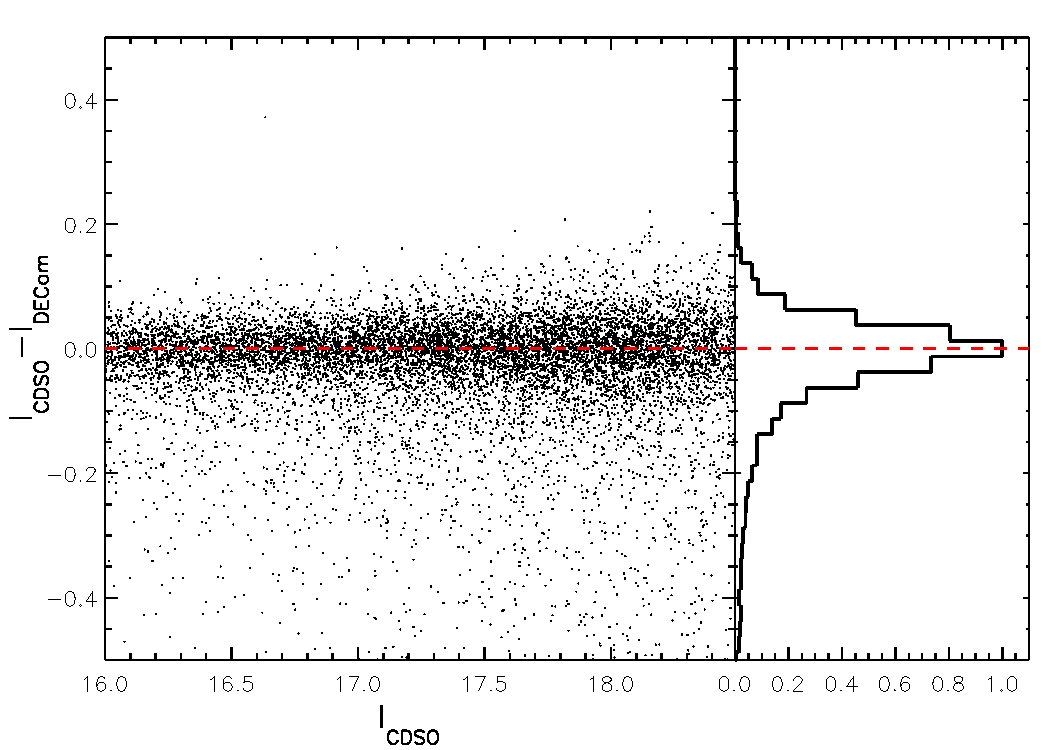
\includegraphics[width=.50\linewidth]{transformation_DECam.pdf}} 
	\end{tabular}
	\caption[Transformation of the DECam photometry to the Cousins system.]{{\bf Left panel:} Residuals between the $I_c$ magnitudes from the CDSO and the $i$ magnitudes from DECam as a function of the $i-z$ colour from DECam and VISTA data in the SDSS system. {\bf Right panel: } Residuals between the $I_c$-band photometries from the CDSO and DECam after applying Transformation \ref{eq_IMF:DECam_CDSO}.}
	\label{fig_IMF:trasformation_DECam_CDSO}
\end{figure*}

\subsection{Appendix: 25 Ori Distance}
\label{sec_app_IMF:distance}

%\vspace*{5ex}
To estimate the 25 Ori distance, we first compiled a list of 334 unique spectroscopically confirmed members of 25 Ori by \citet{Briceno2005,Briceno2007,Downes2014,Downes2015,Suarez2017,Briceno2018}. Then, we cross-matched this list with the BJ18 catalogue to obtain the distances of the confirmed members. This catalogue has the point distance estimate and a measure of the uncertainty for each source with Gaia DR2 parallax, even if it is negative and/or has very low signal-to-noise ratio. The uncertainties are represented by upper and lower limits which contain about 68 per cent (one standard deviation) of the confidence interval. We considered as the uncertainty for each point distance a half of the interval between its upper and lower limits. 90 per cent of the confirmed members of 25 Ori have distances from BJ18 with uncertainties less than 20 per cent. In the left panel of Figure \ref{fig_IMF:cum_dist} we show the cumulative distribution of these distances, which cover a range from 127 to 545 pc (excluding two confirmed members 625 and 777 pc away), but there is a clear concentration of members around the 25 Ori expected distance with 94 per cent of the member between 250 and 450 pc. From these distances we obtained that 25 Ori is 356$\pm$47 pc away, which is consistent with previous studies \citep{Briceno2007,Downes2014,Suarez2017,Briceno2018,Kounkel2018}.

\subsection{Appendix: 25 Ori Extinction}
\label{sec_app_IMF:extinction}

About 96 per cent of the 334 confirmed members of 25 Ori by \citet{Briceno2005,Briceno2007,Downes2014,Downes2015,Suarez2017,Briceno2018} have reported visual extinctions obtained through spectroscopic analysis. In the right panel of Figure \ref{fig_IMF:cum_dist} we show the cumulative distribution of these extinctions, which go up to 1.88 mag (excluding two members with values of 3.53 and 6.29 mag) but more than 93 per cent of the members with reported extinction have values lower than 1 mag. Considering values up to 1.88 mag, the mean extinction of the 25 Ori is 0.35$\pm$0.35 mag. If we consider values lower than 1 mag, the 25 Ori mean extinction is 0.29$\pm$0.26 mag. As expected, both values are consistent with previous studies \citep{Kharchenko2005,Briceno2005,Briceno2007,Downes2014,Suarez2017,Briceno2018}. 

\begin{figure*}
	\centering
	\begin{tabular}{cc}
		\subfloat{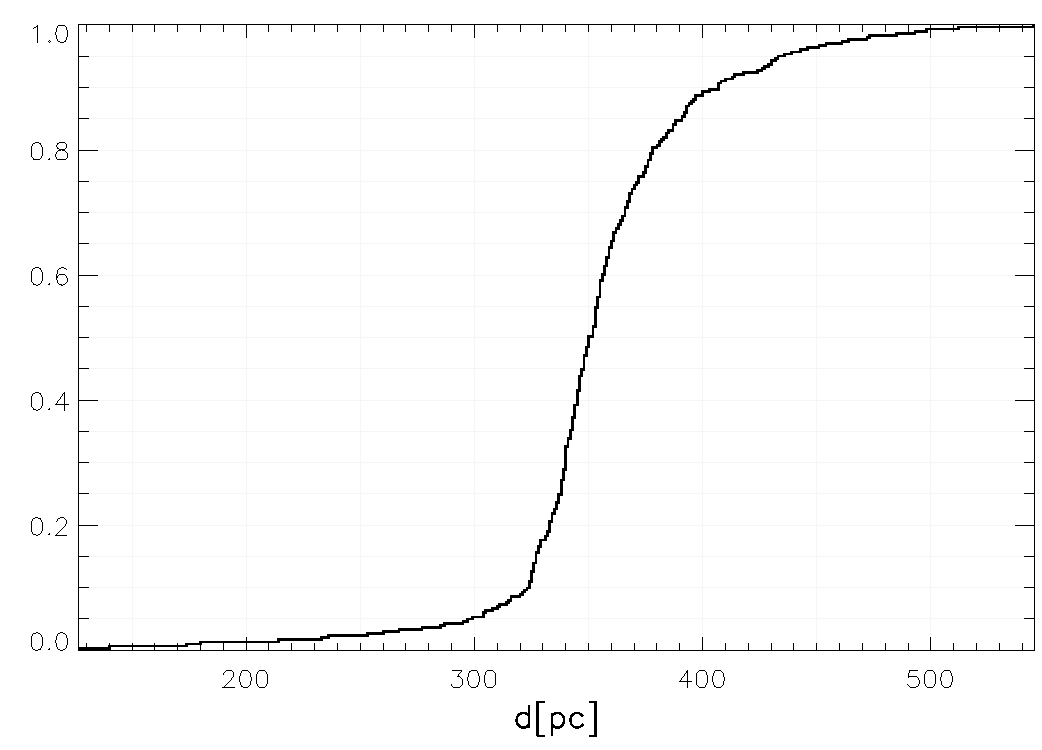
\includegraphics[width=.50\linewidth]{cumulative_distribution_d.pdf}} & 
		\subfloat{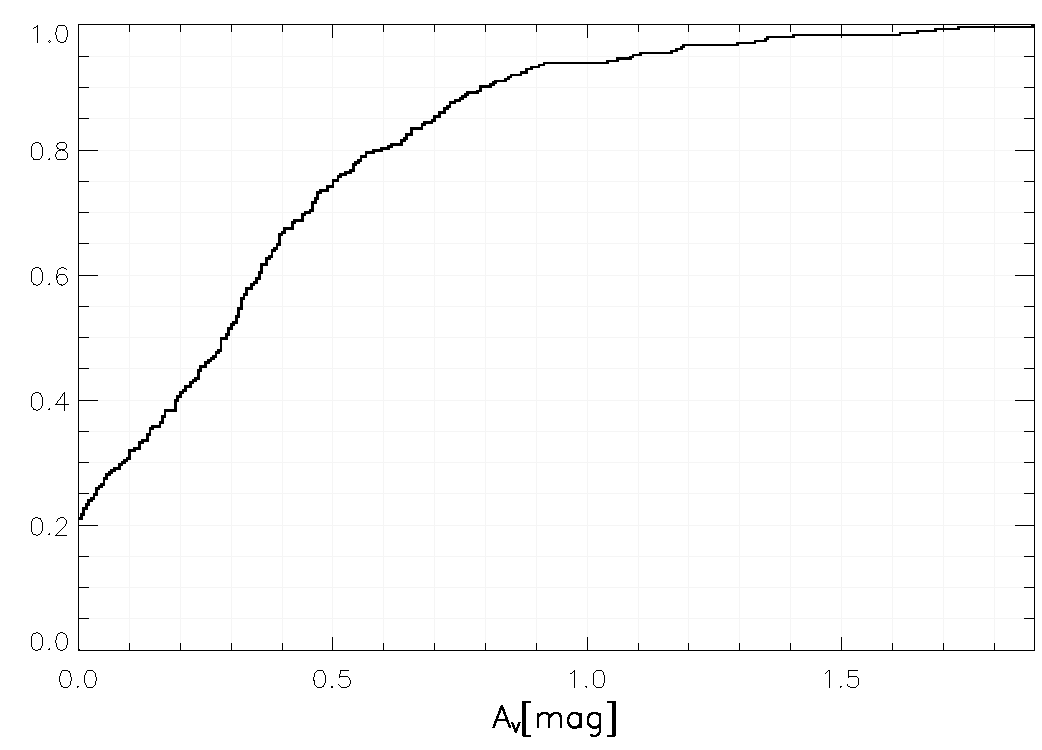
\includegraphics[width=.50\linewidth]{cumulative_distribution_Av.pdf}} 
	\end{tabular}
	\caption[Normalized cumulative distributions of the distances and extinctions of 25 Ori members.]{Normalized cumulative distributions of the distances (left panel) and extinctions (right panel) for the spectroscopically confirmed members of 25 Ori by \citet[][]{Briceno2005,Briceno2007,Downes2014,Downes2015,Suarez2017,Briceno2018}. The distances are from BJ18 and have uncertainties less than 20 per cent. The extinctions were mostly estimated through spectral analysis and combining optical and NIR photometry.}
	\label{fig_IMF:cum_dist}
\end{figure*}

\subsection{Appendix: Distances and Extinctions for the Member Candidates and Contaminants}
\label{sec_app_IMF:distance_extinction}
As we do not have distances and extinctions for all the member candidates (86 per cent have distances and 18 per cent have extinctions) and contaminants, we need to assign these values to the whole samples to have consistency with the 25 Ori members. The most common way to do this in photometric studies in the literature is to consider the mean distance and extinction of the cluster for all the member candidates. Here, we can take advantage of the Gaia DR2 parallaxes as well as of the previous spectroscopic studies in 25 Ori to use a statistically more robust technique. Considering the inversion of the normalized cumulative distribution of the BJ18 distances of the 25 Ori confirmed members (left panel of Figure \ref{fig_IMF:cum_dist}), we created random realizations to assign distance values to all our member candidates and contaminants. We also assigned extinction values to these samples in a similar way, but considering the normalized cumulative distribution of the reported extinctions of the 25 Ori confirmed members (right panel of Figure \ref{fig_IMF:cum_dist}). This way, the distance and extinction values we assigned to each candidate and contaminant are consistent with those for the confirmed members of 25 Ori.


%%%%%%%%%%%%%%%%%%%%%%%%%%%%%%%%%%%%%%%%%
\section{Spectroscopic Follow-Up}
\label{sec:spectroscopy}

\subsection{Research Statement}
\label{sec:rs_spectroscopy}
The analysis in the previous section was done considering photometric member candidates and dealing with the contamination present in the sample in a statistically way. To determine the membership of each source it is necessary a spectroscopy follow-up, which is an arduous observationally work that implies the uses of several world-wide facilities. Having a clear sample of confirmed members is essential to study various astrophysical phenomena as mass segregation, age spreads, evolution of circumstellar disks, and when low-mass stars form respect to the most massive members in the cluster evolution history. 

We have an ongoing spectroscopic survey to observed each 25 Ori member candidate in our sample, which consists of 1687 sources with masses from 10 $M_{Jup}$ to 13 $M_\odot$ distributed in an area of 1.1$^\circ$ radius in 25 Ori. In the following sections we describe our spectroscopic observations and summarize the current state of the survey.

%++++++++++++++++++++++++++++
\subsection{OAN-SPM/MES}
\label{sec:MES}

\subsubsection{MES Spectra}
\label{sec_echelle:spectra}
To observe the brightest 25 Ori candidates we used the Manchester Echelle Spectrograph \citep[MES; ][]{Meaburn1984,Meaburn2003} attached to the 2.1m telescope of the Observatorio Astron\'omico Nacional at San Pedro M\'artir (OAN-SPM) in Mexico, which allows the acquisition of optical high-resolution spectra. We obtained 24 nights of observing time distributed as follow: 6 nights on December 11-16, 2014 (PI: J. J. Downes), 6 nights on January 06-11, 2015 (PI: J. J. Downes), 6 nights on October 24-29, 2015 (PI: G. Su\'arez) and 6 nights on January 22-27, 2016 (PI: G. Su\'arez). In Table \ref{tab:MES_log} we show the log of our MES observations.
%MES is a single slit spectrograph that uses interference filter to isolote the spectral orders of interest. 

\subsubsubsection{Target Selection}
\label{sec_echelle:targets}
The selection of the MES targets was done on the basis of their positions in the $V$ vs $V-J$ and $H$ vs $H-K$ diagrams using the UCAC4 and 2MASS catalogs. We defined the empirical isochrone traced by the spectroscopically confirmed members by \citet{Briceno2005,Briceno2007,Downes2014} as well as the highly probable members by \citet{Kharchenko2005}. Then, we defined the PMS locus as the region around the empirical isochrone and containing most of the confirmed and highly probable members, and selected the sources lying inside both loci. Additionally, we removed from the candidate selection the sources having low photometric and kinematics probability of being members according to \citet{Kharchenko2005}. The final sample contains 80 member candidates covering an area of 3x3 deg$^2$ around 25 Ori and with $V$-band magnitudes from 4.9 to 12.1, which corresponds to the mass range from 1.6 to 13.1 M$_\odot$ considering the PARSEC-COLIBRI 7 Myr isochrone.

\subsubsubsection{Data Reduction}
\label{sec_echelle:reduction}
During our MES observations we obtained spectra of 77 of these member candidates (96\% of the sample), including all those lying inside the 1.0$^\circ$ radius area of 25 Ori. Additionally, we obtained images for the calibration of the data (bias, flats, ThAr lamps and radial velocity standards). To reduced the spectra we used the standard \texttt{IRAF}\footnote{IRAF is distributed by the National Optical Astronomy Observatory, which is operated by the Association of Universities for Research in Astronomy (AURA) under a cooperative agreement with the National Science Foundation.} tasks to remove bias, flats and cosmic rays, and to extract the spectra, calibrate in wavelength and normalize the continuum. The final wavelength covered by the 32 orders (from 32 to 63) in each spectra ranges from 3600 to 7100 \AA\ with a typical resolution of $R=21000$ at H$_\alpha$. In Figure \ref{fig_MES:spectrum} we show an example of a MES spectrum, focusing in some orders of interest.

\subsubsection{Membership Assignment}
\label{sec_MES:membership}
The radial velocities (RVs) of the spectra were obtained using the $fxcor$ task of \texttt{IRAF}, which correlates the spectra with unknown radial velocity with a templete spectrum with known radial velocity. For this correlation we considered the following absorption lines: H$_\alpha$ (in order 34), NaI$\lambda\lambda$5890, 5896 (in order 38), MgI$\lambda\lambda\lambda$5167, 5172, 5184 (in order 43), H$_\beta$ (in order 46), CaII$\lambda$3968 (in order 56) and CaII$\lambda$3934 (in order 57). So far, we have obtained radial velocities for 22 targets of the sample (about 30\%) which have values between 10 and 40 km s$^{-1}$ (plus two targets with values of -10 and 50 km s$^{-1}$) and with typical uncertainties of 3 km s$^{-1}$. 

To determine which of these targets are members of 25 Ori, we applied criteria on the basis of their radial velocities, distances and spatial distribution as follow:

$i)$ First, we cross matched our list of targets with Gaia DR2 \citep{GaiaCollaboration2018}; 99\% of all the MES targets have reliable parallaxes (errors lesser than 20\%). To filter the sample according to their distances, we considered the 25 Ori distance of $356\pm47$ pc (Su\'arez et al. 2018, submitted) and selected the targets located around 25 Ori with a dispersion of $3\sigma$. About 86\% of the MES targets satisfies this criterion. 

$ii)$ Additionally, we selected the targets with radial velocities between 10 and 40 km s$^{-1}$ to have consistency with 25 Ori \citep{Briceno2007}. From the 22 targets with radial velocity from the MES spectra, 14 sources satisfy the distance and radial velocity criteria. 

$iii)$ Finally, we selected the sources lying inside the 25 Ori estimated area of 1.0$^\circ$ radius. From the 14 targets with distance and radial velocity consistent with 25 Ori, 10 of them are located inside the 25 Ori limits.

In summary, from the 22 targets with radial velocity from the MES spectra and with distances from Gaia DR2, 10 of them have spatial distribution, distances and radial velocities consistent with 25 Ori. Therefore, from the entire sample of MES spectra (77 targets) we roughly expect 36 intermediate/high mass members of 25 Ori. %In Figure \ref{} we show the radial velocity distribution for the targets with measurements.
%Assuming the 25 Ori system IMF by Su\'arez et al. (2018, in prep.), we expect 

\begin{table} \tiny
\begin{center}
 \caption[OAN-SPM/MES observing log]{OAN-SPM/MES observing log.}
 \label{tab:MES_log}
 \begin{threeparttable}
  	\setlength{\tabcolsep}{11pt}
	\begin{tabular}{lccccccl}
	\toprule
	{\bf Target} & {\bf RA}    & {\bf DEC}    & {\bf UT Date}        & {\bf Airmass} & {\bf T$_{exp}$} & $V$     &  {\bf Comments} \\
	             & (hh:mm:ss)  & (hh:mm:ss)   &(yyyy-mm-ddThh:mm:ss) &               & (s)             & (mag)   &                 \\
	\midrule
	\multicolumn{8}{c}{{\bf 2014B Runs}} \\
	25Ori\_40     & 05:23:14.54 & +02:01:06.9 & 2014-12-11T05:20:32  & 1.415         & 3000             & 11.627 & tiny clouds              \\
	25Ori\_65     & 05:23:45.91 & +01:50:33.4 & 2014-12-11T06:43:46  & 1.189         & 2000             & 9.923  & ---                      \\
	25Ori\_93     & 05:24:16.19 & +01:38:35.7 & 2014-12-11T08:31:15  & 1.168         & 3000             & 11.442 & bad sky                  \\
	25Ori\_86     & 05:24:12.73 & +01:34:12.1 & 2014-12-11T10:35:36  & 1.541         & 3000             & 10.645 & ---                      \\
	25Ori\_105    & 05:24:20.74 & +01:35:26.6 & 2014-12-12T05:27:09  & 1.382         & 6000             & 9.793  & ---                      \\
	25Ori\_128    & 05:24:44.83 & +01:50:47.2 & 2014-12-12T07:27:03  & 1.148         & 2000             & 4.878  & a second spectrum 		\\
	25Ori\_256    & 05:26:11.98 & +01:53:35.7 & 2014-12-12T09:13:14  & 1.233         & 3000             & 9.33   & ---                      \\
	25Ori\_157    & 05:25:11.65 & +01:33:29.7 & 2014-12-12T10:37:16  & 1.571         & 3000             & 9.959  & ---                      \\
	25Ori\_134    & 05:24:54.56 & +01:58:08.3 & 2014-12-12T11:53:37  & 2.428         & 2000             & 10.064 & ---                      \\
	25Ori\_265    & 05:26:19.93 & +01:47:14.3 & 2014-12-13T08:52:49  & 1.203         & 3600             & 12.183 & ---                      \\
	25Ori\_235    & 05:26:03.68 & +01:48:29.4 & 2014-12-13T11:03:39  & 1.792         & 3600             & 10.81  & ---                      \\
	25Ori\_66     & 05:23:50.20 & +01:32:52.9 & 2014-12-14T05:07:48  & 1.43          & 3000             & 10.586 & ---                      \\
	25Ori\_123    & 05:24:38.92 & +01:54:06.4 & 2014-12-14T06:54:42  & 1.163         & 3000             & 10.969 & ---                      \\
	25Ori\_135    & 05:24:55.01 & +01:39:22.9 & 2014-12-14T08:24:08  & 1.172         & 3600             & 11.128 & ---                      \\
	25Ori\_99     & 05:24:18.17 & +02:22:06.1 & 2014-12-14T09:59:35  & 1.402         & 3000             & 10.091 & ---                      \\
	25Ori\_95     & 05:24:17.61 & +02:22:04.6 & 2014-12-14T10:57:04  & 1.766         & 2000             & 9.572  & very close to 25Ori 99   \\
	\multicolumn{8}{c}{{\bf 2015A Runs}} \\
	25Ori\_487    & 05:28:45.29 & +01:38:38.1 & 2015-01-07T08:21:37  & 1.381         & 3000             & 6.895  & ---                      \\
	25Ori\_547    & 05:29:33.53 & +03:08:52.5 & 2015-01-07T09:44:31  & 1.912         & 3000             & 7.104  & ---                      \\
	25Ori\_668    & 05:31:29.89 & +01:41:24.1 & 2015-01-10T03:50:59  & 1.34          & 1200             & 7.517  & ---                      \\
	25Ori\_447    & 05:28:15.70 & +01:34:48.2 & 2015-01-10T04:43:42  & 1.202         & 1200             & 8.983  & ---                      \\
	25Ori\_390    & 05:27:20.59 & +02:12:57.1 & 2015-01-10T05:37:06  & 1.144         & 5100             & 9.171  & ---                      \\
	25Ori\_512    & 05:28:59.36 & +01:29:19.1 & 2015-01-10T08:18:19  & 1.418         & 2700             & 9.293  & ---                      \\
	25Ori\_586    & 05:30:08.82 & +01:14:52.4 & 2015-01-10T09:20:03  & 1.831         & 2700             & 9.339  & ---                      \\
	25Ori\_119    & 05:24:36.10 & +02:21:11.4 & 2015-01-11T03:55:13  & 1.283         & 600              & 6.307  & ---                      \\
	25Ori\_577    & 05:30:02.85 & +01:06:33.3 & 2015-01-11T04:42:35  & 1.207         & 2700             & 9.577  & ---                      \\
	25Ori\_435    & 05:28:01.47 & +01:17:53.7 & 2015-01-11T05:32:49  & 1.154         & 600              & 6.388  & ---                      \\
	\multicolumn{8}{c}{{\bf 2015B Runs}} \\
	25Ori\_121    & 05:24:36.62 & +01:48:03.5 & 2015-10-24T07:30:36  & 1.832         & 3000             & 8.948  & ---                      \\
	25Ori\_122    & 05:24:38.62 & +01:48:38.8 & 2015-10-24T08:48:06  & 1.352         & 3000             & 8.311  & ---                      \\
	25Ori\_152    & 05:25:11.10 & +01:52:01.6 & 2015-10-24T10:02:56  & 1.178         & 3000             & 9.86   & ---                      \\
	25Ori\_80     & 05:24:07.86 & +01:38:00.1 & 2015-10-25T06:38:40  & 2.537         & 3000             & 9.339  & ---                      \\
	25Ori\_30     & 05:23:01.94 & +01:41:48.9 & 2015-10-25T07:59:12  & 1.565         & 3000             & 8.135  & ---                      \\
	25Ori\_24     & 05:22:47.96 & +01:43:00.2 & 2015-10-25T09:17:39  & 1.249         & 3000             & 9.641  & ---                      \\
	25Ori\_318    & 05:26:48.11 & +02:04:05.8 & 2015-10-25T11:01:57  & 1.143         & 3000             & 8.503  & ---                      \\
	25Ori\_148    & 05:25:10.30 & +01:15:31.3 & 2015-10-26T06:49:30  & 2.292         & 3000             & 9.839  & ---                      \\
	25Ori\_377    & 05:27:19.20 & +01:36:22.4 & 2015-10-26T08:00:01  & 1.563         & 3000             & 8.88   & ---                      \\
	25Ori\_146    & 05:25:07.39 & +00:56:00.7 & 2015-10-26T09:20:16  & 1.249         & 4800             & 9.587  & tiny clouds              \\
	25Ori\_69     & 05:23:51.38 & +00:51:46.3 & 2015-10-26T11:03:19  & 1.158         & 3000             & 8.388  & ---                      \\
	25Ori\_569    & 05:29:54.77 & +01:47:21.3 & 2015-10-26T12:04:15  & 1.199         & 900              & 5.749  & ---                      \\
	25Ori\_242    & 05:26:06.00 & +00:50:02.4 & 2015-10-27T06:40:48  & 2.416         & 3000             & 8.298  & ---                      \\
	25Ori\_281    & 05:26:27.20 & +00:50:21.2 & 2015-10-27T07:54:30  & 1.585         & 3600             & 9.892  & ---                      \\
	25Ori\_238    & 05:26:04.62 & +00:43:38.9 & 2015-10-27T09:14:33  & 1.258         & 3600             & 9.215  & ---                      \\
	25Ori\_538    & 05:29:28.64 & +01:43:09.7 & 2015-10-27T10:37:29  & 1.148         & 4500             & 10.215 & ---                      \\
	25Ori\_131    & 05:24:50.10 & +00:45:58.6 & 2015-10-27T12:23:28  & 1.271         & 3000             & 8.71   & ---                      \\
	25Ori\_126    & 05:24:42.80 & +01:43:48.2 & 2015-10-28T07:44:00  & 1.596         & 3600             & 10.258 & ---                      \\
	25Ori\_111    & 05:24:24.21 & +01:41:33.3 & 2015-10-28T09:18:06  & 1.226         & 3600             & 10.233 & ---                      \\
	25Ori\_210    & 05:25:47.02 & +00:31:12.9 & 2015-10-29T07:46:24  & 1.588         & 900              & 6.149  & ---                      \\
	25Ori\_425    & 05:27:54.23 & +01:06:18.2 & 2015-10-29T08:14:59  & 1.432         & 1350             & 7.79   & ---                      \\
	25Ori\_570    & 05:29:55.56 & +02:08:31.8 & 2015-10-29T08:54:10  & 1.312         & 1800             & 8.144  & ---                      \\
	25Ori\_211    & 05:25:48.66 & +01:23:22.0 & 2015-10-29T10:07:23  & 1.161         & 2700             & 10.424 & ---                      \\
	25Ori\_468    & 05:28:34.15 & +00:45:57.6 & 2015-10-29T11:09:37  & 1.166         & 900              & 9.719  & low SNR                  \\
	\multicolumn{8}{c}{{\bf 2016A Runs}} \\
	25Ori\_494    & 05:28:48.46 & +02:09:53.0 & 2016-01-22T03:18:54  & 1.28          & 3000             & 7.136  & ---                      \\
	25Ori\_440    & 05:28:10.12 & +00:47:14.0 & 2016-01-22T04:46:04  & 1.162         & 3000             & 8.35   & ---                      \\
	25Ori\_601    & 05:30:29.60 & +01:46:55.4 & 2016-01-22T06:06:02  & 1.182         & 4000             & 10.214 & ---                      \\
	25Ori\_513    & 05:28:59.71 & +03:21:48.6 & 2016-01-22T07:35:12  & 1.401         & 4000             & 10.343 & ---                      \\
	25Ori\_571    & 05:29:55.94 & +02:12:34.0 & 2016-01-22T09:29:49  & 2.655         & 3000             & 10.36  & ---                      \\
	25Ori\_630    & 05:30:53.05 & +01:36:47.0 & 2016-01-23T02:51:07  & 1.375         & 4000             & 10.512 & ---                      \\
	25Ori\_652    & 05:31:13.56 & +01:23:12.0 & 2016-01-23T04:23:15  & 1.171         & 4000             & 10.561 & ---                      \\
	25Ori\_548    & 05:29:34.26 & +01:53:50.5 & 2016-01-23T06:06:35  & 1.187         & 4000             & 10.633 & ---                      \\
	25Ori\_222    & 05:25:50.76 & +00:47:48.9 & 2016-01-23T08:26:34  & 1.853         & 4000             & 10.737 & tiny clouds              \\
	25Ori\_473    & 05:28:36.30 & +02:20:42.9 & 2016-01-24T03:00:01  & 1.31          & 4000             & 10.686 & close companion         \\
	25Ori\_466    & 05:28:31.17 & +01:54:07.8 & 2016-01-24T04:34:53  & 1.151         & 4000             & 10.764 & ---                      \\
	25Ori\_428    & 05:27:57.33 & +02:16:34.6 & 2016-01-24T05:42:52  & 1.161         & 4000             & 10.782 & ---                      \\
	25Ori\_454    & 05:28:18.74 & +01:20:56.1 & 2016-01-24T08:32:11  & 1.909         & 4000             & 10.805 & ---                      \\
	25Ori\_486    & 05:28:44.05 & +01:11:37.9 & 2016-01-25T02:44:04  & 1.371         & 4000             & 10.806 & ---                      \\
	25Ori\_542    & 05:29:30.65 & +01:29:41.0 & 2016-01-25T04:11:24  & 1.171         & 4000             & 10.872 & ---                      \\
	25Ori\_137    & 05:25:00.18 & +01:38:29.8 & 2016-01-25T05:58:41  & 1.197         & 4000             & 10.876 & close companions         \\
	25Ori\_396    & 05:27:33.26 & +01:12:55.1 & 2016-01-25T06:52:28  & 1.322         & 6000             & 10.882 & tiny clouds              \\
	25Ori\_467    & 05:28:33.18 & +01:45:55.9 & 2016-01-25T09:09:34  & 2.521         & 4000             & 10.964 & tiny clouds              \\
	25Ori\_472    & 05:28:35.44 & +01:40:07.3 & 2016-01-26T02:55:07  & 1.311         & 4000             & 10.983 & ---                      \\
	25Ori\_469    & 05:28:34.40 & +02:20:18.2 & 2016-01-26T04:41:44  & 1.141         & 4000             & 11.014 & ---                      \\
	25Ori\_554    & 05:29:38.03 & +01:56:05.6 & 2016-01-26T06:01:41  & 1.197         & 4000             & 11.081 & close companion          \\
	25Ori\_445    & 05:28:15.32 & +01:27:34.1 & 2016-01-26T07:36:17  & 1.524         & 5000             & 11.27  & ---                      \\
	25Ori\_309    & 05:26:46.56 & +01:40:55.2 & 2016-01-26T09:02:14  & 2.496         & 3000             & 11.358 & ---                      \\
	25Ori\_94     & 05:24:17.49 & +01:38:30.1 & 2016-01-27T02:58:00  & 1.279         & 4800             & 11.366 & ---                      \\
	25Ori\_492    & 05:28:47.46 & +02:18:51.1 & 2016-01-27T04:20:38  & 1.148         & 4800             & 11.37  & ---                      \\
	25Ori\_239    & 05:26:04.90 & +00:32:19.7 & 2016-01-27T06:25:23  & 1.28          & 4800             & 11.419 & ---                      \\
	25Ori\_308    & 05:26:45.90 & +03:26:54.0 & 2016-01-27T07:45:46  & 1.574         & 4800             & 11.448 & ---                      \\
	\bottomrule
	\end{tabular}
%	\begin{tablenotes}[para,flushleft]
%	  $^a$ Less time than requested but the spectra have enough SNR for our analysis.\\
%	\end{tablenotes}
 \end{threeparttable}
\end{center}
\end{table}

\begin{figure*}[ht!]
	\centering
	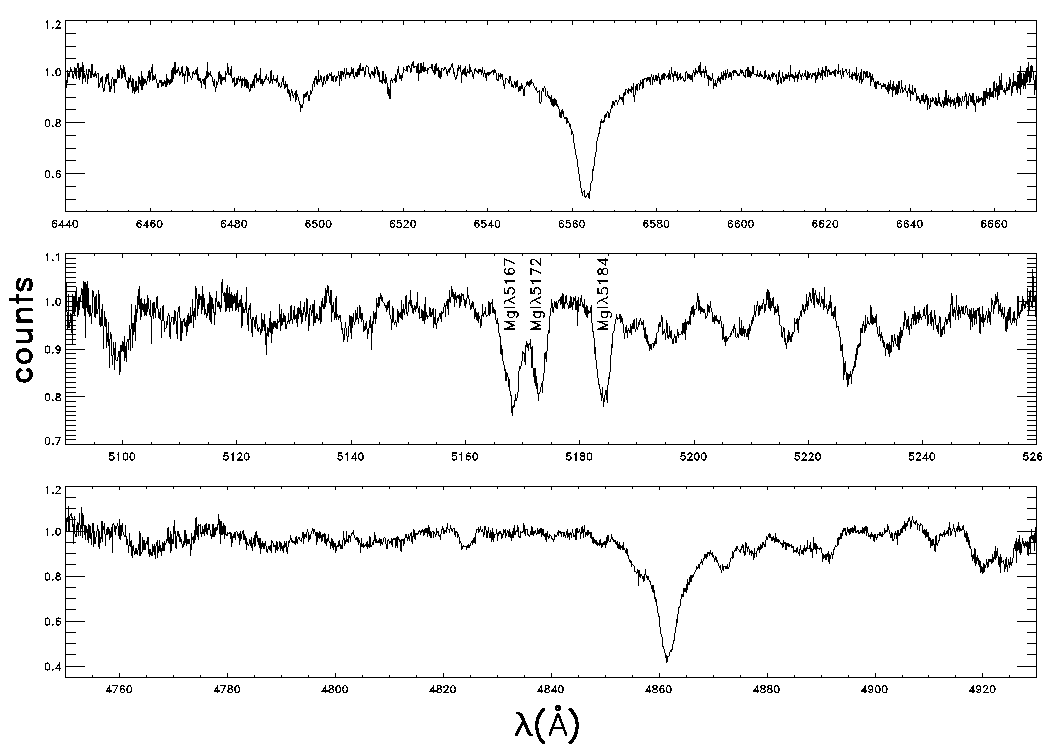
\includegraphics[width=1.\textwidth]{MES_spectrum.pdf}
	\caption[MES spectrum of a confirmed member of 25 Ori]{MES spectrum of a confirmed member of 25 Ori. The panels show the absorption of the lines: H$_\alpha$ (in order 34; upper panel), MgI$\lambda\lambda\lambda$5167, 5172, 5184 (in order 43; middle panel) and H$_\beta$ (in order 46; lower panel).}
	\label{fig_MES:spectrum}
\end{figure*}

\subsubsection{Physical Parameters}
\label{sec_MES:membership}
To calculate the $T_{eff}$ of all the MES spectra we first plan to use the SPTCLASS code to obtain the spectral types to then convert them to $T_{eff}$ using the \citet{Kenyon-Hartmann1995} or \citet{Pecaut2013} relations. By now, we estimated $T_{eff}$ of the member candidates by interpolating their observed $G-J$ color from Gaia DR2 and 2MASS in an updated version of the \citet{Kenyon-Hartmann1995} relation, assuming the $A_V$ of 25 Ori obtained in this work ($0.29\pm0.26$ mag). For the estimation of $L_{bol}$, mass and age we used the routine described in Section \ref{sec_APOGEE-2:physical_parameters}, working with the PARSEC-COLIBRI isochrones. The masses obtained for the sources range between 1.3 and 11 $M_\odot$.

%++++++++++++++++++++++++++++
\subsection{SDSS-IV/APOGEE-2}
\label{sec:APOGEE-2}

\subsubsection{APOGEE-2 Spectra}
\label{sec_APOGEE-2:spectra}
To observe 25 Ori member candidates less masive that those observed with the MES spectrograph and with expected masses larger than the peak of the IMF (0.30 $M_\odot$; Su\'arez et al. 2018, submitted), we used the Apache Point Observatory Galactic Evolution Experiment 2 (APOGEE-2) spectrograph, mounted on the 2.5m SDSS telescope \citep{Gunn2006,Blanton2017}. As one of the SDSS-IV programs, APOGEE-2 is a multi-fiber spectrograph that allows the acquisition of up to 300 moderate-to-high resolution ($R\sim22500$) spectra at the $H$-band (1.51-1.70 $\mu$m) across a 1.5$^\circ$ radius FOV \citep{Wilson2010,Majewski2017}. We obtained, as part of the APOGEE-2 Young Cluster Survey, two high-priority plates with 10 visits dedicated to the observation of mainly 25 Ori targets. In Table \ref{tab:APOGEE-2_fields} we summarize the details of these APOGEE-2 fields in 25 Ori. Each visit contains spectra of about 250 scientific targets.

\begin{table} \tiny
\begin{center}
 \caption{APOGEE-2 fields in 25 Ori.}
 \label{tab:APOGEE-2_fields}
 \begin{threeparttable}
  	\setlength{\tabcolsep}{11pt}
	\begin{tabular}{lcccccc}
	\toprule
	{\bf Field Name} & {\bf RA}    & {\bf DEC}  & {\bf Plate ID} & {\bf Epoch} & {\bf UT Date}         & Seeing   \\
	                 & ($^\circ$) & ($^\circ$)  &                & (MJD)       & (yyyy-mm-ddThh:mm:ss) & (arcsec) \\
	\midrule
	Ori OB1ab-E & 81.496 & 1.006 & 8900 & 2457648 & 2016-09-17T11:01:08.967 & 1.4 \\
	            &        &       & 8901 & 2457649 & 2016-09-18T11:24:21.106 & 1.4 \\
	            &        &       & 8901 & 2457650 & 2016-09-19T11:22:07.462 & 1.4 \\
	            &        &       & 8902 & 2457652 & 2016-09-21T11:59:29.344 & 1.4 \\
	            &        &       & 8902 & 2457653 & 2016-09-22T11:10:54.354 & 1.8 \\
	            &        &       & 8903 & 2457675 & 2016-10-14T10:17:16.340 & 1.6 \\
	\midrule
	Ori OB1ab-F & 82.000 & 3.000 & 8904 & 2457676 & 2016-10-15T10:53:52.447 & 1.5 \\
	            &        &       & 8905 & 2457410 & 2016-01-23T04:27:33.611 & 1.5 \\
	            &        &       & 8906 & 2457411 & 2016-01-24T04:24:59.808 & 1.4 \\
	            &        &       & 8906 & 2457412 & 2016-01-25T04:55:00.687 & 2.1 \\
	\bottomrule
	\end{tabular}
%	\begin{tablenotes}[para,flushleft]
%	  $^a$ Less time than requested but the spectra have enough SNR for our analysis.\\
%	\end{tablenotes}
 \end{threeparttable}
\end{center}
\end{table}

\subsubsubsection{Target Selection}
\label{sec_APOGEE-2:targets}
The selection of the targets was based on IR excess, variability and color-magnitude criteria as well as including previously confirmed member and X-ray sources, as explained in \citet{Cottle2018} and summarized as followed:

$i)$ For a uniform selection of young stellar objects (YSOs) with IR excess, the \cite{Koenig2014} method was followed considering near- and mid-IR (NIR, MID) photometry from the 2MASS and WISE \citep{Cutri2013} catalogs, respectively, which provides an efficiency of about 80\%, proven in $\sigma$ Ori and $\lambda$ Ori \citep{Koenig2015}. 

$ii)$ Additionally, to extend the uniform selection of YSOs, including diskless sources, we considered variable candidates, which is an effective method for the selection of PMS stars \citep{Briceno2005,Briceno2018}, using the PanSTARRS catalog \citep{Chambers2016}. 

$iii)$ The number of YSOs selected from IR excess and variability criteria requiered about 10\% of the available APOGEE-2 fibers, therefore, we filled the rest of the fibers with previously confirmed members by \citet{Briceno2005,Briceno2007,Downes2014,Suarez2017} and highly probable member from \citet{Kharchenko2005}, X-ray sources from the 3XMM-DR5 catalog \citep{Rosen2015} and member candidates selected on the basis of their position in $I$ vs $I-J$ diagrams using photometry from the USNO \citep{Monet2003} and 2MASS catalogs. For the selection of these member candidates we considered the sources lying inside the defined PMS locus working with the empirical isochrone traced by several spectroscopically confirmed members and highly probable members of 25 Ori and Orion OB1a. In Figure \ref{fig_APOGEE-2:targets_selection} we show the CMDs for the selection of photometric candidates observed with APOGEE-2 in 25 Ori. 

In Table \ref{tab_APOGEE-2:targets} we summarize the number of APOGEE-2 targets selected from the above criteria and keeping all of them with $H$-band magnitudes between 7. and 12.2, to ensure signal-to-noise ratio (SNR) $>100$ for a three-visit source with a total of 3h of exposure \citep{Majewski2017}. We prioritized the targets to first assign fibers to the uniformly selected sources and then to the rest of the candidates. After removing duplicates and 72'' fiber collisions, we acquired 1185 unique APOGEE-2 spectra in both plates dedicated to 25 Ori. In Figure \ref{fig_APOGEE-2:sky} we show the spatial distribution of these APOGEE-2 targets.

\begin{figure*}
	\centering
	\begin{tabular}{cc}
		\subfloat{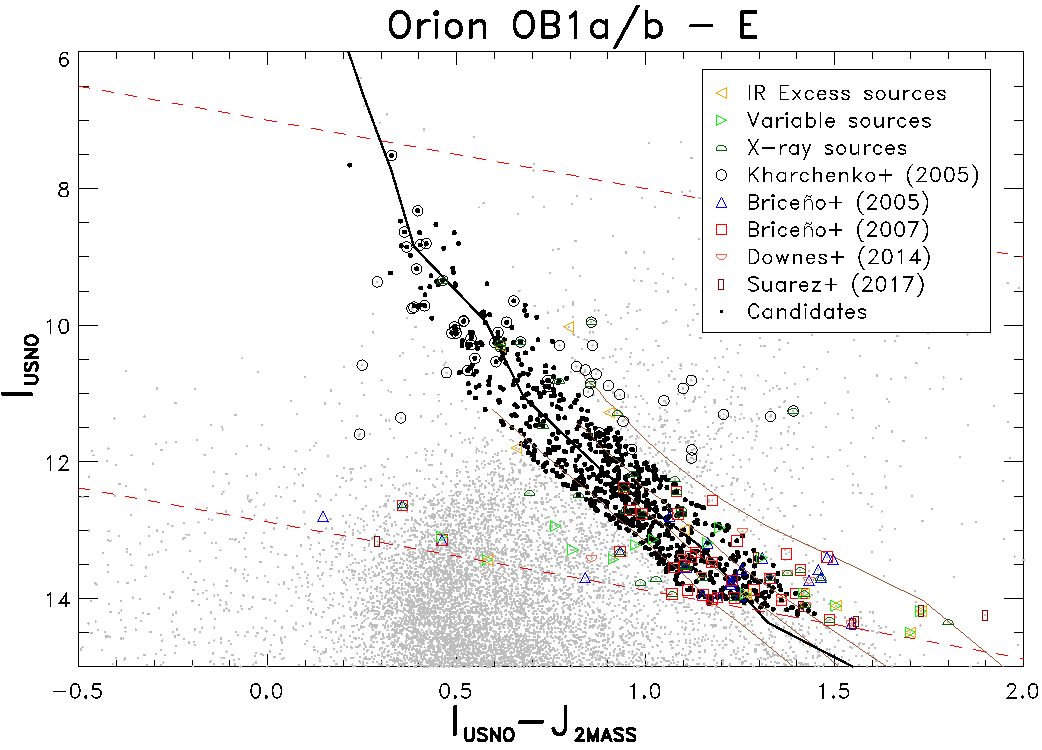
\includegraphics[width=.50\linewidth]{CMD_plate_E.pdf}} & 
		\subfloat{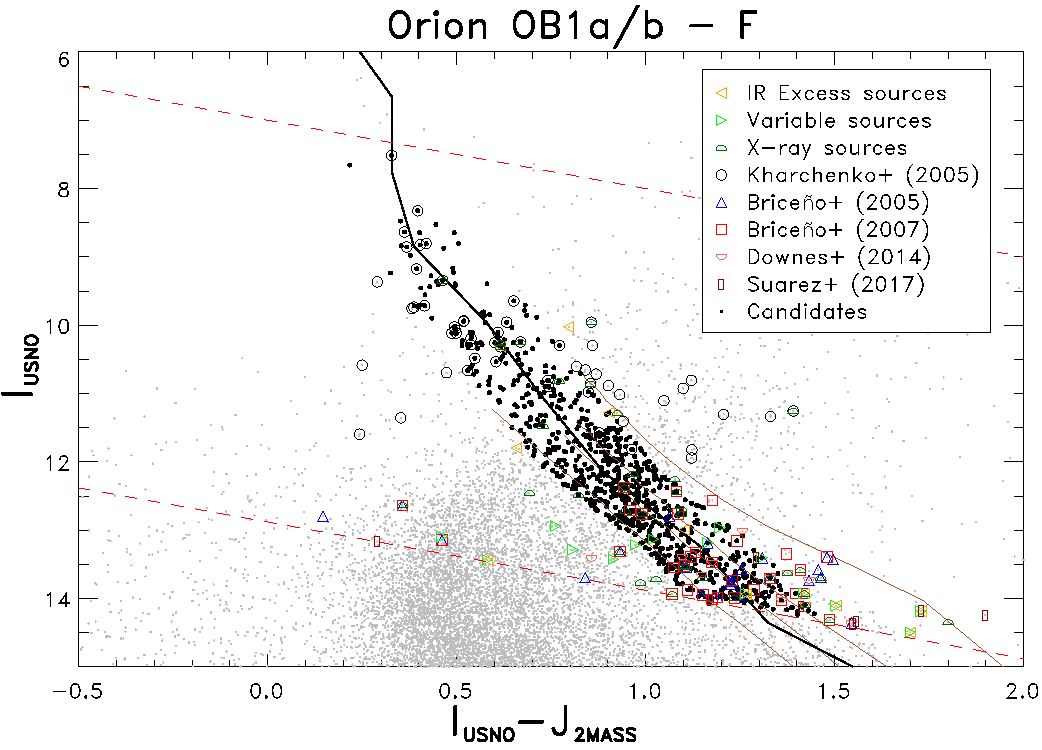
\includegraphics[width=.50\linewidth]{CMD_plate_F.pdf}}
	\end{tabular}
	\caption[CMD for the selection APOGEE-2 targets.]{CMDs used to select member candidates (black points) for the APOGEE-2 plates dedicated to 25 Ori (OB1ab-E in left panel and OB1ab-F in right panel). The open symbols show confirmed members, highly probable members and member candidates of 25 Ori and Orion OB1a, as indicated in the label. The black solid curve corresponds to the empirical isochrone and the brown curves represent the BT-Settl isochrones for 1, 3, 5 and 10 Myr. The red dashed lines indicate the APOGEE-2 limits of 7 and 12.2 mag in the $H$-band. 
	\label{fig_APOGEE-2:targets_selection}}
\end{figure*}

\begin{table} \scriptsize
\begin{center}
 \caption{APOGEE-2 targets in 25 Ori.}
 \label{tab_APOGEE-2:targets}
 \begin{threeparttable}
  	%\setlength{\tabcolsep}{11pt}
	\begin{tabular}{@{\extracolsep{2pt}}cccccccccc}
	\toprule
	\multicolumn{2}{c}{{\bf IR Excess}} & \multicolumn{2}{c}{{\bf Variable}} & \multicolumn{2}{c}{{\bf X-ray sources}} & \multicolumn{2}{c}{{\bf Members}$^a$} & \multicolumn{2}{c}{{\bf Candidates}} \\
   	\cline{1-2}
   	\cline{3-4}
   	\cline{5-6}
   	\cline{7-8}
   	\cline{9-10}
	{\bf Selected} & {\bf Observed}     & {\bf Selected} & {\bf Observed}    & {\bf Selected} & {\bf Observed}         & {\bf Selected} & {\bf Observed}       & {\bf Selected} & {\bf Observed}      \\
	\midrule
	23 & 20 & 28 & 25 & 40 & 38 & 216 & 92 & 1442 & 985 \\
	\bottomrule
	\end{tabular}
	\begin{tablenotes}[para,flushleft]
	  $^a$ Spectroscopically confirmed members considering the studies by \citet{Briceno2005,Briceno2007,Downes2014,Suarez2017}.\\
	\end{tablenotes}
 \end{threeparttable}
\end{center}
\end{table}

\begin{figure*}%[ht!]
	\centering
	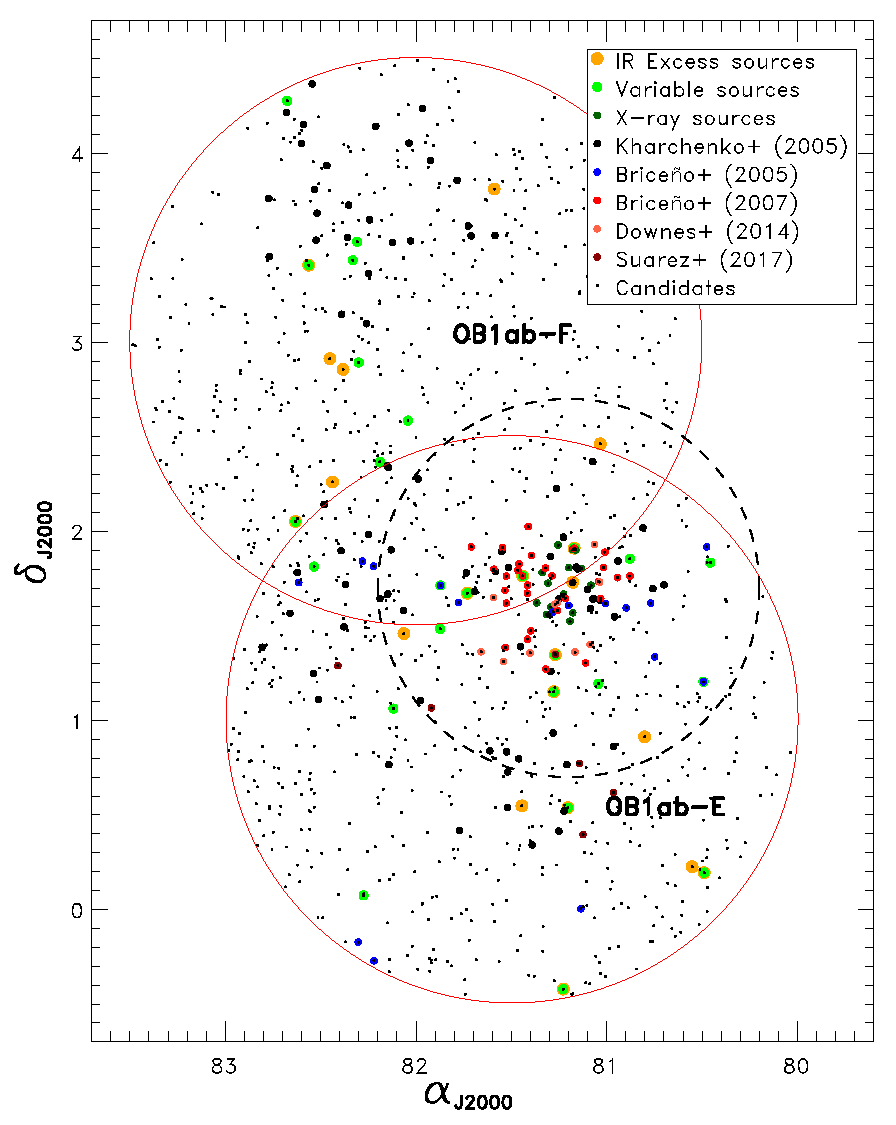
\includegraphics[width=1.\textwidth]{sky_APOGEE-2.pdf}
	\caption[Spatial distribution of the targets observed by APOGEE-2 in 25 Ori]{Spatial distribution of the targets observed by APOGEE-2 in the two plates dedicated to 25 Ori (red circles). The colored points represent the different kind of targets and the sizes indicate their priority, as shown in the label. The dashed circle shows the 1$^\circ$ radius area of 25 Ori.}
	\label{fig_APOGEE-2:sky}
\end{figure*}

\subsubsubsection{Radial Velocities and Effective Temperatures}
\label{sec_APOGEE-2:targets}
We downloaded the APOGEE-2 spectra from the Science Archive Sever, which are available for SDSS-IV members. These spectra were originally processed by the APOGEE Stellar Parameter and Chemical Abundances Pipeline \citep[ASPCAP; ][]{GarciaPerez2016}, which is an automated software for the determination of RV, $T_{eff}$, surface gravity (log $g$) and chemical abundances with accuracies of $\sim$0.1 km s$^{-1}$, 2\%, 0.1 dex and $\lesssim0.05$ dex, respectively, through a comparison of the observed spectra to libraries of theoretical spectra. However, ASPCAP is optimized for the analysis of spectra of red giant stars and can introduce biases when working with spectra of YSOs \citep{Nidever2015}. Therefore, these APOGEE-2 spectra were processed by \citet{Kounkel2018} using the pipeline developed by \citet{Cottaar2014}, which is designed for spectra of PMS stars. This pipeline determines the $T_{eff}$, log $g$, RV, rotational velocity ($v$ sin $i$) and $H$-band veiling ($r_H$) for each source by fitting the observed spectra to synthetic spectra and minimizing $\chi^2$. The corresponding uncertainties are derived by the pipeline by Markov chain Monte Carlo (MCMC) simulations. After some comparisons between the results using the \citet{Coelho2005}, \citet{Allard2012} and \citet[PHOENIX; ][]{Husser2013} spectral libraries assuming solar metallicities, the adopted parameters are from PHOENIX because produce the most self-consistent solutions and covers the widest $T_{eff}$ range (2300-15000 K) \citep{Kounkel2018}. These fits were done for each visit spectrum and then, the reported parameters for each target are the weighted average of the parameters in all the visits for that specific target. Additionally to the use of this pipeline, we are working with the TONALLI code (Adame et al. 2018, in preparation) to fit the PHOENIX synthetic spectra to the observed spectra considering $\alpha$ element (O, Ne, Mg, Si, S, Ar, Ca and Ti) abundance ([$\alpha/$Fe]) and [Fe/H] as free parameters. This is a ongoing work and therefore, for the following analysis, we used the parameters derived by \citet{Kounkel2018}. 

Particularly, the parameters of interest for this project from the APOGEE-2 spectra are $T_{eff}$ and RV. For the APOGEE-2 plates in 25 Ori, the typical $T_{eff}$ uncertainties are 40 K but significantly increase for sources with $T_{eff}>6250$ K. For the RV errors, the typical values are 0.5 km s$^{-1}$.

\subsubsection{Spectra Analysis}
\label{sec_APOGEE-2:analysis}

\subsubsubsection{Membership Assignment}
\label{sec_APOGEE-2:memberships}
As in the APOGEE-2 targets is present contamination from background and, in a lesser degree, from foreground field stars, to select the 25 Ori members we applied distance, RV and spatial distribution criteria, similarly than for the MES spectra, to have consistent values with those expected for the 25 Ori population. About 90\% of all the targets in plates Ori OB1ab-E and OB1ab-F have reliable BJ18 distances (errors less than 20\%) and there are 353 sources satisfying the distance and RV criteria, of which 153 lie inside the 1$^\circ$ radius area of 25 Ori. This sample of 25 Ori members covers $H$-band mangitudes between 8.4 and 12.2, which corresponds to the mass range from 0.6 to 3.7 $M_\odot$, considering the PARSEC-COLIBRI 7 Myr isochrone. From these 153 members in 25 Ori, 56 of them have been confirmed before through spectroscopic studies by \citet[18 sources; ][]{Briceno2005}, \citet[9 sources; ][]{Briceno2007}, \citet[8 sources; ][]{Downes2014}, \citet[3 sources; ][]{Suarez2017} and \citet[18 sources; ][]{Briceno2018}, which have $H$-band magnitudes fainter than 10.6 (1.3 $M_\odot$). Therefore, we confirmed here, using APOGEE-2 spectra, 97 new members of 25 Ori,% with masses $0.6\lesssim m/M_\odot \lesssim 3.7$.
%Additionally, 32 of our confirmed members have high-probability of being members according to \citet{Kharchenko2005}.

There are 9 additional previously confirmed 25 Ori members with APOGEE-2 spectra that we did not recover after applying our membership criteria; 2 of them because have distances of $180\pm2$ and $545\pm87$ pc and the remaining 7 members becuase do not have Gaia DR2 parallax (4 sources) or their parallaxes or RVs have errors larger than 20\% (3 sources).

In Figure \ref{fig_APOGEE-2:rv} we show the radial velocity distributions of all the APOGEE-2 targets lying inside 25 Ori ($1^\circ$ radius area) and for the distance filtered targets as well as for the previously confirmed members. The most prominent peak corresponds to the 25 Ori population and has a mean value of $20.9\pm2.0$ km s$^{-1}$, considering the previously confirmed members with APOGEE-2 RVs or from the APOGEE-2 targets filtered by their distances and removing the sources with RV larger than 28 km s$^{-1}$. This mean RV and the dispersion are pretty consistent with that obtained by \citet[$19.7\pm1.7$ km s$^{-1}$; ][ and references therein]{Briceno2007} with a smaller sample of 47 members of 25 Ori. The second peak at about 28 km s$^{-1}$ can be do to the dispersed OB1a population or even to overlapping members of OB1b \citep[Orion C and D; ][]{Kounkel2018}, which have RVs of $\sim24$ \citep{Jeffries2006} and $30.1\pm1.9$ km s$^{-1}$ \citep{Briceno2007}, respectively.

\begin{figure*}%[ht!]
	\centering
	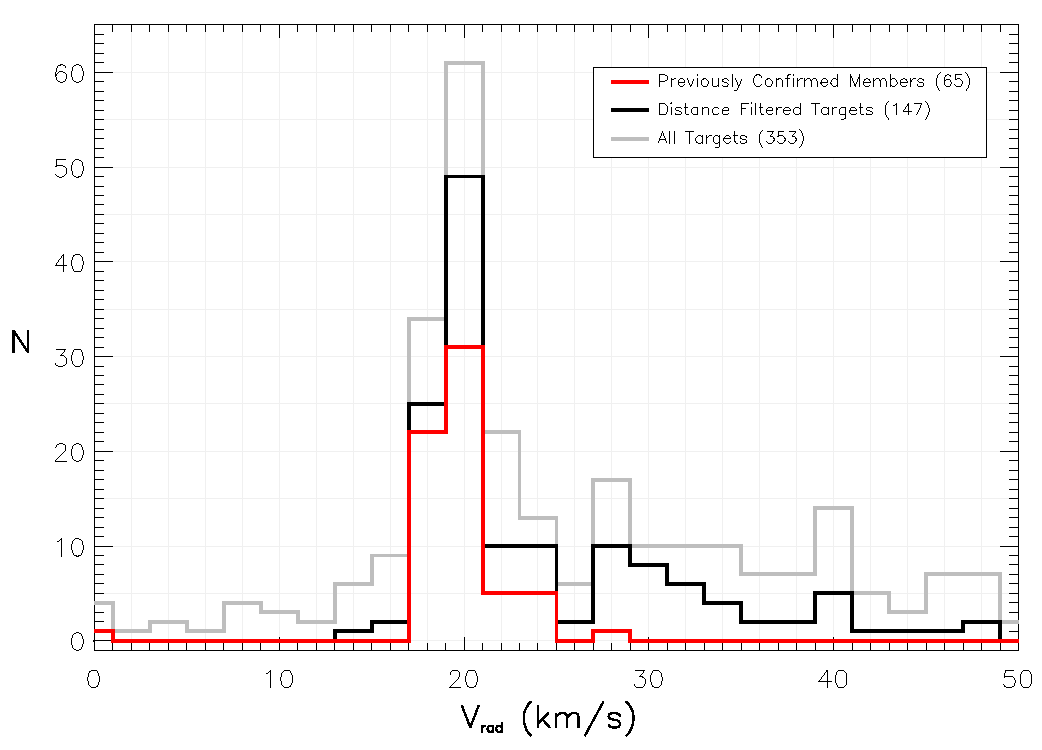
\includegraphics[width=1.\textwidth]{radial_velocity.pdf}
	\caption[Radial velocity distributions of the APOGEE-2 targets and members of 25 Ori.]{Radial velocity distributions of all the APOGEE-2 targets inside 25 Ori (grey histogram), of the targets after applying the distance criterion (black histrogram) and of the spectroscopically confirmed members in the literature with RV from APOGEE-2 (red histogram).}
	\label{fig_APOGEE-2:rv}
\end{figure*}

\subsubsubsection{Physical Parameters}
\label{sec_APOGEE-2:physical_parameters}
After we applied the membership criteria to the APOGEE-2 spectra in plates OB1ab-E and OB1ab-F, we estimated the physical parameters of interest for the resulting 25 Ori members. For this purpose, we developed a specific routine.

\paragraph{PHYPAR Routine\\}
\label{sec_APOGEE-2:phypar}
%For the estimation of the bolometric luminosity (\ac{Lbol}), mass and age of young stellar and substellar objects, I developed the {\href{https://drive.google.com/open?id=1uNv7nxVas2F0TOz3q5aJsKD8yVd4FwqG}{\texttt{PHYPAR}}} IDL routine. The input parameters are distance, $T_{eff}$, $A_V$, and a photometric band magnitude together with their uncertainties. So far, the code works with magnitudes in the $G$, $V$, $R$, $I$, $J$, $H$ or $K$ photometric bands.
For the estimation of the bolometric luminosity (\ac{Lbol}), mass and age of young stellar and substellar objects, I developed the PHYPAR IDL routine (see Appendix \ref{sec_app:phypar}), which has been succesfully tested in several contributions \citep{Suarez2017,Kounkel2018,Ramirez-Preciado2018}. The input parameters are distance, $T_{eff}$, $A_V$, and a photometric band magnitude together with their uncertainties. So far, the code works with magnitudes in the $G$, $V$, $R$, $I$, $J$, $H$ or $K$ photometric bands.

First, the magnitudes are dereddened by assuming, depending of the band of the input magnitudes, the \citet{Cardelli1989} coefficients or $C_G=0.9145$ (J. Hern\'andez, private communication) and then the distance modulus is added to obtain the absolute magnitudes. These magnitudes are converted to bolometric magnitudes using the bolometric corrections obtained by interpolating $T_{eff}$ in the \citet{Kenyon-Hartmann1995} relation combined with the \citet{Luhman1999}, \citet{Briceno2002} and \citet{Luhman2003b} relations for the LMSs and BDs. Then, the bolemetric magnitudes are converted to $L_{bol}$. Finally, $T_{eff}$ and $L_{bol}$ are interpolated into stellar models to obtain masses and ages for the sources lying inside a defined region of the models. This region is defined according to the expected masses and ages of the sources, which avoid degeneracy when the stellar model also includes the post-MS. The code uses the BT-Settl or PARSEC-COLIBRI isochrones, which allows to cover a wide mass range (from planetary masses to tend of solar masses) for sources in the PMS or MS.

The errors for each parameter are obtained as follow: $i)$ when each of the above steps involve an equation, the uncertainties are computed using the corresponding error propagation rule and $ii)$ when an interpolation is done, the error is defined as the standard deviation of the resultant values from the interpolation of 10$^3$ generated numbers following a normal distribution centered at the parameter value and with a standard deviation equal to one third its error (this way 99.7\% of the random values are within the uncertainties).

%{\href{https://drive.google.com/open?id=1uNv7nxVas2F0TOz3q5aJsKD8yVd4FwqG}{\texttt{PHYPAR}}} IDL routine I developed, which has been succesfully tested in several contributions \citep{Suarez2017,Kounkel2018,Ramirez-Preciado2018}. The input parameters are distance, $T_{eff}$, $A_V$, and a photometric band magnitude together with their uncertainties. First, the magnitudes are dereddened by assuming the \citet{Cardelli1989} coefficients for the 2MASS photometric bands and the above mentioned Gaia coefficient to then add the distance modulus to obtain the absolute magnitudes. These magnitudes are converted to bolometric magnitudes using the bolometric corrections (BCs) obtained by interpolating $T_{eff}$ in the \citet{Kenyon-Hartmann1995} relation and then are converted to $L_{bol}$. Finally, $T_{eff}$ and $L_{bol}$ are interpolated into stellar models to obtain masses and ages for the members lying inside a defined region of the models. The errors for each parameter are obtained as follow: $i)$ when each of the above steps involve an equation, the uncertainties are computed using the corresponding error propagation rule and $ii)$ when an interpolation is done, the error is defined as the standard deviation of the resultant values from the interpolation of 10$^3$ generated numbers following a normal distribution centered at the parameter value and with a standard deviation equal to one third its error (this way 99.7\% of the random values are within the uncertainties). So far, the code works with magnitudes in the $V$, $G$, $J$, $H$ or $K$ photometric bands and with the BT-Settl or PARSEC-COLIBRI isochrones.

\paragraph{Parameters\\}
\label{sec_APOGEE-2:parameters}
Before using the PHYPAR code for the resulting confirmed memebers, we estimated $A_V$ considering photometry from the Gaia DR2 and 2MASS catalogs and $T_{eff}$ from the APOGEE-2 spectra. We compared the observed $G-J$ and $G_{BP}-G_{RP}$ colors with the intrinsic colors obtained by interpolating $T_{eff}$ into the PARSEC-COLIBRI 7 Myr isochrone and then transforming the color excesses to $A_V$. When resulting a negative extinction, which can be due to the $T_{eff}$ errors and/or magnitude uncertainties, we assigned null values. We computed the $A_V$ uncertainties similarly than explained in previous section. For most of the sources, the $A_V$ values obtained using only Gaia DR2 photometry are in agreement with those combining Gaia DR2 with 2MASS. The resultant $A_V$ from the Gaia DR2 photometry are in the range from 0 to 1.8 mag, but most of them ($\approx$75\%) have values lesser than 1 mag. The mean extinction, $\bar{A}_V$, we obtained is $0.39\pm0.40$ mag, without considering sources with unexpected values. This low extinction is consistent with previous works (Su\'arez et al. 2018, submitted and references therein).
%assuming the coefficients $C_{G_{BP}}=1.039$, $C_G=0.9145$, $C_{G_{RP}}=0.601$ and $C_J=0.282$ (\citealt{Cardelli1989} and J. Hern\'andez, private communication)

%To estimate the bolometric luminosity (\ac{Lbol}), mass and age for each confirmed member, we used the {\href{https://drive.google.com/open?id=1uNv7nxVas2F0TOz3q5aJsKD8yVd4FwqG}{\texttt{PHYPAR}}} IDL routine I developed, which has been succesfully tested in several contributions \citep{Suarez2017,Kounkel2018,Ramirez-Preciado2018}. The input parameters are distance, $T_{eff}$, $A_V$, and a photometric band ($V$, $G$, $J$, $H$ or $K$) together with their uncertainties. First, the magnitudes are dereddened by assuming the \citet{Cardelli1989} coefficients for the 2MASS photometric bands and the above mentioned Gaia coefficient to then add the distance modulus to obtain the absolute magnitudes. These magnitudes are converted to bolometric magnitudes using the bolometric corrections (BCs) obtained by interpolating $T_{eff}$ in the \citet{Kenyon-Hartmann1995} relation and then are converted to $L_{bol}$. Finally, $T_{eff}$ and $L_{bol}$ are interpolated into stellar models to obtain masses and ages for the members lying inside a defined region of the models. The errors for each parameter are obtained as follow: $i)$ when each of the above steps involve an equation, the uncertainties are computed using the corresponding error propagation rule and $ii)$ when an interpolation is done, the error is defined as the standard deviation of the resultant values from the interpolation of 10$^3$ generated numbers following a normal distribution centered at the parameter value and with a standard deviation equal to one third its error (this way 99.7\% of the random values are within the uncertainties).

Then, the $L_{bol}$, mass and age of the APOGEE-2 members were obtained using the PHYPAR routine with distances from BJ18, $T_{eff}$ from the APOGEE-2 spectra, $A_V$ derived here from the Gaia DR2 photometry and $G$ magnitudes from Gaia DR2 as well as the PARSEC-COLIBRI isochrones. In Figure \ref{fig_APOGEE-2:HR} we show the H-R diagram of the members from the APOGEE-2 spectra. The masses of these members in 25 Ori ranges between 0.3 and 5.2 $M_\odot$. The mean age we obtained is $7.2\pm3.6$ Myr, which is pretty consistent with previous studies in 25 Ori \citep[][ and references therein]{Briceno2018}.

\begin{figure*}[ht!]
	\centering
	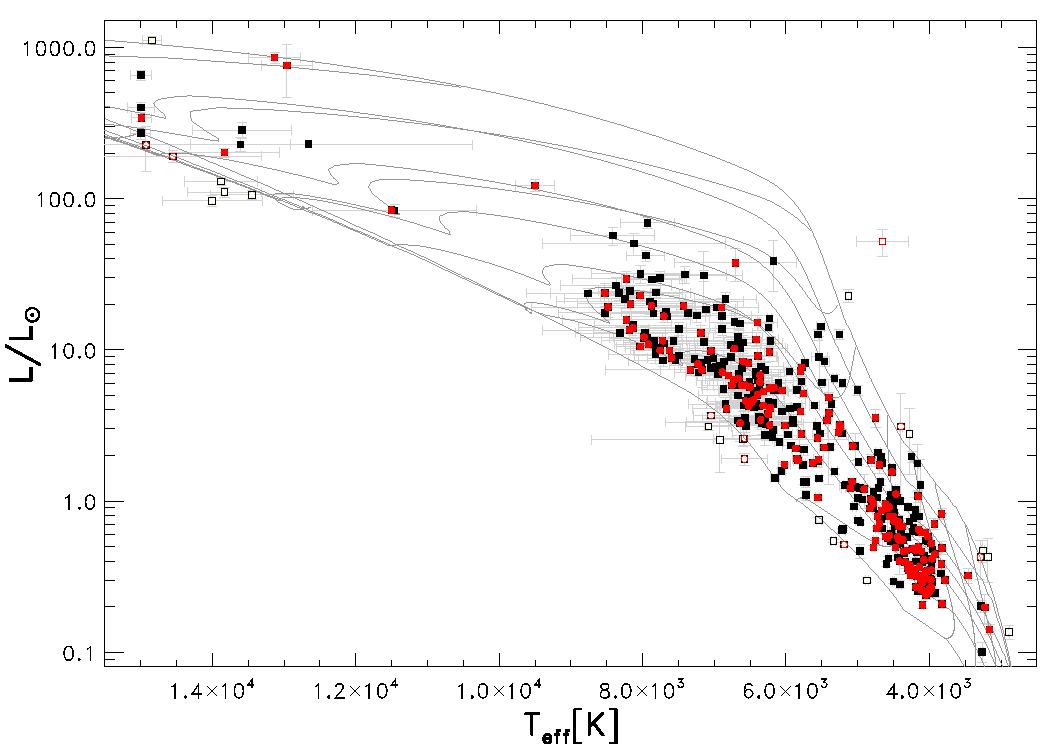
\includegraphics[width=1.\textwidth]{HR_APOGEE-2.pdf}
	\caption[H-R diagram of the 25 Ori confirmed members from APOGEE-2 spectra.]{H-R diagram of the confirmed members in the APOGEE-2 OB1ab-E and OB1ab-F plates (black squares) and of the members lying inside the 25 Ori area of $1^\circ$ radius (red circles). The grey curves represent the PARSEC evolutionary tracks for 0.3, 0.5, 0.7, 1.0, 2.0, 3.0, 4.0 and 5.0 $M_\odot$ and the PARSEC-COLIBRI isocrones for 0.5, 1, 2, 3, 5, 10 and 30 Myr. The open symbols indicate the members without mass and age estimates because they lie outside the model grid.}
	\label{fig_APOGEE-2:HR}
\end{figure*}

\subsection{SDSS-III/BOSS \citep{Suarez2017}}
\label{sec:BOSS}
The following analysis of a set of spectra from the BOSS spectrograph constitute the publication by \citet{Suarez2017}.

%\begin{figure*}[ht!]
%	\centering
%	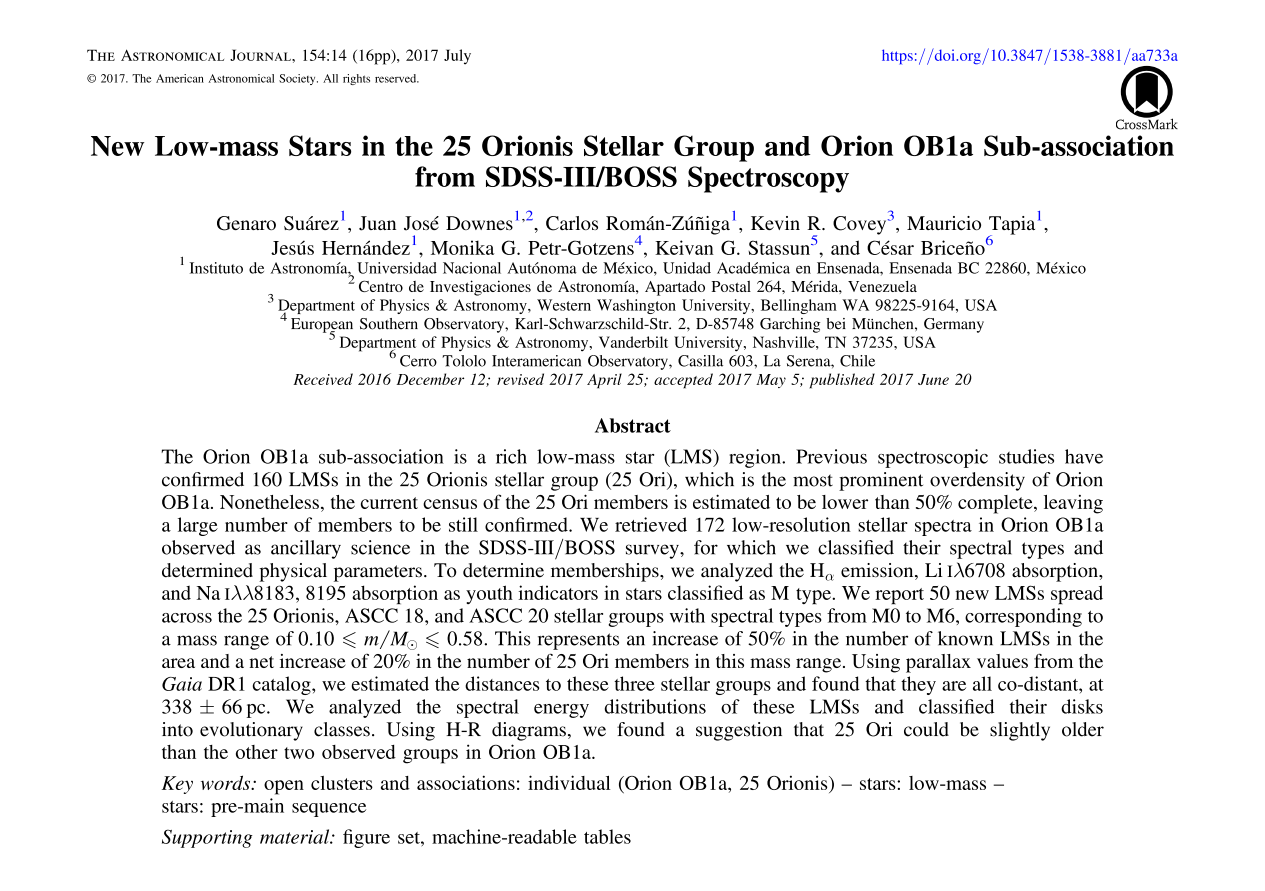
\includegraphics[width=1.\textwidth]{BOSS_paper.png}
%	\caption[]{.}
%	\label{fig_BOSS:paper}
%\end{figure*}

{\bf Abstract.}
The Orion OB1a sub-association is a rich low mass star (LMS) region. Previous spectroscopic studies have confirmed 160 LMSs in the 25 Orionis stellar group (25 Ori), which is the most prominent overdensity of Orion OB1a. Nonetheless, the current census of the 25 Ori members is estimated to be less than 50\% complete, leaving a large number of members to be still confirmed. We retrieved 172 low-resolution stellar spectra in Orion OB1a observed as ancillary science in the SDSS-III/BOSS survey, for which we classified their spectral types and determined physical parameters. To determine memberships, we analyzed the H$_\alpha$ emission, LiI$\lambda$6708 absorption, and NaI$\lambda\lambda$8183, 8195 absorption as youth indicators in stars classified as M-type. We report 50 new LMSs spread across the 25 Orionis, ASCC 18, and ASCC 20 stellar groups with spectral types from M0 to M6, corresponding to a mass range of 0.10$\le m/\textrm{M}_\odot \le$0.58. This represents an increase of 50\% in the number of known LMSs in the area and a net increase of 20\% in the number of 25 Ori members in this mass range. Using parallax values from the Gaia DR1 catalog, we estimated the distances to these three stellar groups and found that they are all co-distant, at 338$\pm$66 pc. We analyzed the spectral energy distributions of these LMSs and classified their disks by evolutionary classes. Using H-R diagrams, we found a suggestion that 25 Ori could be slightly older that the other two observed groups in Orion OB1a.

\subsubsection{Introduction}
\label{sec_BOSS:intro}
Comprehensive studies of known OB associations in terms of their stellar populations and structural properties provide a firm basis to the understanding of how young star aggregations form and evolve until they eventually disperse to be part of the Galactic disk component. Particularly useful in this respect are the $\sim 10$ Myr {\it fossil star forming regions} \citep[FSFRs; ][]{Blaauw1991}, where one would expect that: \textit{i}) the dust and gas are largely dispersed, and extinction is generally low, permitting the detection of low mass stars (LMSs), \textit{ii}) the members are still spatially concentrated and can be distinguished from the field population, \textit{iii}) only a minority of stars retain optically thick circumstellar disks, \textit{iv}) the active star formation was ceased but its products are still present, \textit{v}) accretion is essentially over, so the objects have attained their final masses, and \textit{vi}) the stars can be considered nearly coeval.

The properties of the LMSs in the FSFRs are of particular importance to understand/clarify the structure and dispersal processes acting on such stellar populations, the circumstellar disk evolution and the possible large-scale dynamical effects. In fact, such studies are not possible solely from the observation of massive stars, as the LMSs do have relatively large pre-main-sequence (PMS) phases, they are characterized by the presence of evolving disks, variable mass accretion and circumstellar and chromospheric activity. Furthermore, they make up the majority of all the stars formed in clusters in terms of number and mass \citep[e.g.,][]{Bastian2010}, and have long lifetimes ($>10^{10}$ yr) in the main sequence (MS).

The Orion OB1 association is one of the largest and nearest star forming regions \citep[e.g. ][]{Genzel-Stutzki1989,Bally2008,Briceno2008} and contains four distinct sub-associations, which can be distinguished according to their ages and content of gas and dust \citep{Blaauw1964}. With an age of 7-10 Myr and a distance of $\sim$330 pc \citep[e.g.,][]{Briceno2005}, Orion OB1a is the oldest and closest of the Orion OB1 sub-associations. Considering the critical age of 10 Myr, Orion OB1a is an excellent region for studying the early evolution of LMSs. Particularly important is the 25 Orionis stellar group (25 Ori), one of the most numerous and spatially dense 7-10 Myr old populations (r$\sim7$ pc, $\Sigma \sim 128$ stars deg$^{-2}$) known within 500 pc from the Sun \citep{Briceno2007}. 

As mentioned in \citet{Downes2014}, there are other associations of similar age to 25 Ori, but these regions cover relatively extended areas in the sky or are too distant to enable the detection of their LMSs. 25 Ori's unique combination of its distance, age, and area in the sky \citep[360 pc, $\sim7$ Myr, and $\approx 3$ deg$^2$; ][]{Briceno2005,Briceno2007,Downes2014}, makes it a particularly convenient region for studying the population of LMSs. Additionally, 25 Ori is almost free of extinction \citep[$A_V\approx0.30$ mag.; ][]{Kharchenko2005,Briceno2005,Briceno2007,Downes2014}.

Although 25 Ori is a clear spatial overdensity of young LMSs \citep{Briceno2007,Downes2014}, a level of contamination is expected close to 25 Ori from at least two other nearby 10 Myr old stellar groups, identified as ASCC 18 and ASCC 20 by \citet{Kharchenko2005,Kharchenko2013}. Thus, in order to disentangle these groups and identify the complete 25 Ori population, it is necessary to make a study that covers an area into those additional groups, beyond the proposed 25 Ori radius of $1^\circ$ \citep{Briceno2005,Briceno2007}.

Several spectroscopic studies have confirmed, to date, 160 LMS members of 25 Ori \citep{Briceno2005,Briceno2007,Biazzo2011,Downes2014,Downes2015}, which represent about 34\% of its total estimated LMS members \citep{Downes2014}. In this paper, we analyze optical spectra obtained with the SDSS-III/BOSS spectrograph to confirm 50 additional young LMSs in Orion OB1a, of which 22 are inside the 25 Ori's estimated area \citep[$1^\circ$ radius; ][]{Briceno2005,Briceno2007}. This increases the confirmed member sample of 25 Ori by about 20\% in a mass range from 0.1 to 0.6 M$_\odot$. We characterize these new members according to their optical spectral types and spectral features, as well as infrared (IR) photometric signatures of circumstellar disks. The paper is organized as follows: In Section \ref{sec_BOSS:observations} we describe the optical and IR photometric data, and the optical spectroscopy from the SDSS-III/BOSS survey. In Section \ref{sec_BOSS:results} we analyze the spectra and describe our results. In Section \ref{sec_BOSS:singular} we comment on particular objects and in Section \ref{sec_BOSS:summary} we discuss and summarize the results.

\subsubsection{Observations}
\label{sec_BOSS:observations}

\subsubsubsection{Optical Photometry}
\label{sec_BOSS:Optphot}
The $V$, $R$, and $I$ photometry used in this work was obtained from the CIDA Deep Survey of Orion (CDSO) catalog \citep{Downes2014}, which was constructed by co-adding the multi-epoch optical observations from the CIDA Variability Survey of Orion \citep[CVSO; ][]{Briceno2005,Mateu2012}. The sensitivity limits of the CDSO covers the LMS and brown dwarf (BD) population of 25 Ori and its surroundings within the region $79.7^\circ\lesssim\alpha\lesssim82.7^\circ$ and $0.35^\circ\lesssim\delta\lesssim3.35^\circ$. The limiting magnitude of the CDSO photometry in this region is $I_{lim}=22$ and the completeness magnitude is $I_{com}=19.6$ \citep{Downes2014}, enough to assure an $I$ band detection even for the faintest targets of our spectroscopic sample ($I\approx17.0$).

Additionally, we used the $u$, $g$, $r$, $i$, and $z$ photometry from the Sloan Digital Sky Survey (SDSS) catalog \citep[][]{Finkbeiner2004,Ahn2012}. These values are listed in Table \ref{tab_BOSS:photometry}.

\subsubsubsection{IR Photometry}
\label{sec_BOSS:IRphot}
The \textit{Z, Y, J, H,} and \textit{Ks} near-IR photometry used in this study was carried out by \citet{Petr-Gotzens2011} as part of the Visible and Infrared Survey Telescope for Astronomy (VISTA) science verification surveys \citep{Arnaboldi2010}. The 5$\sigma$ limiting magnitudes of the VISTA survey of the Orion star-forming region are $Z=22.5$, $Y=21.2$, $J=20.4$, $H=19.4$, and $Ks=18.6$, which are enough to have VISTA photometry even for the faintest objects in our spectroscopic sample ($J\approx15.0$).

Additionally, we used near-IR photometry from the 2MASS catalog \citep{Skrutskie2006} and mid-IR photometry from IRAC-\textit{Spitzer} \citep[][]{Hernandez2007b} and the WISE All-Sky catalog \citep{Cutri2013}. This IR photometry is listed in Table \ref{tab_BOSS:photometry}.

\subsubsubsection{Spectroscopy}
\label{sec_BOSS:spectroscopy}
The spectra used in this paper were obtained as part of the Baryon Oscillation Spectroscopic Survey \citep[BOSS; ][]{Dawson2013}, which is one of the four main surveys of SDSS \citep[][]{York2000} in its third phase \citep[SDSS-III; ][]{Eisenstein2011}. The BOSS spectrograph has plates with 1000 fibers of 2'' diameter spanning a field of view of 3.0$^\circ$ in diameter and cover a wavelength range from 3560 \AA\ to 10400 \AA\ with a resolution of R=1560 at 3700 \AA\ and R=2650 at 9000 \AA \citep{Gunn2006,Smee2013}. 

The spectra we analyzed were obtained as part of the {\it Star Formation in the Orion and Taurus Molecular Clouds} ancillary science program \citep{Alam2015}. The plate is centered around the B2 star 25 Orionis ($\alpha_{J2000}= 5^{\rm h} 24^{\rm m} 44^{\rm s}$.8; $\delta_{J2000} = +1^{\circ} 50' 47''.2$) and includes the stellar groups ASCC 16 (25 Ori), ASCC 18, and ASCC 20 \citep{Kharchenko2013}. The object selection process for this plate is described in detail in Section A2 by \citet{Alam2015} and is based on the cataloged optical and IR photometric properties (SDSS, WISE, 2MASS, Spitzer) of the objects. The integration time for the selected objects was 5 x 4500 s, achieving a typical S/N ratio of $\sim$20 for the faintest sources. The observation produced 677 spectra of which only 172 are stellar and the remaining 505 turned out to be spectra of galaxies and quasars, as explained in Section \ref{sec_BOSS:results}. In Figure \ref{fig_BOSS:sky} we show the spatial distribution of the targets observed in this plate \citep{Alam2015}, as well as the locations of the different stellar groups from \citet{Kharchenko2013}. In Figure \ref{fig_BOSS:CCD_bias} we show the $u-K$ vs $K$-W3 color-color diagram including all the targets of the 25 Ori BOSS plate, where we can see that most of these targets have $K$-W3 colors redder than those expected from previously confirmed members. It is important to notice that this target selection implies a bias towards sources with IR excesses (e.g. stars with accretion disks, see Section \ref{sec_BOSS:TTSclass}).

\begin{figure*}[ht!]
	\centering
	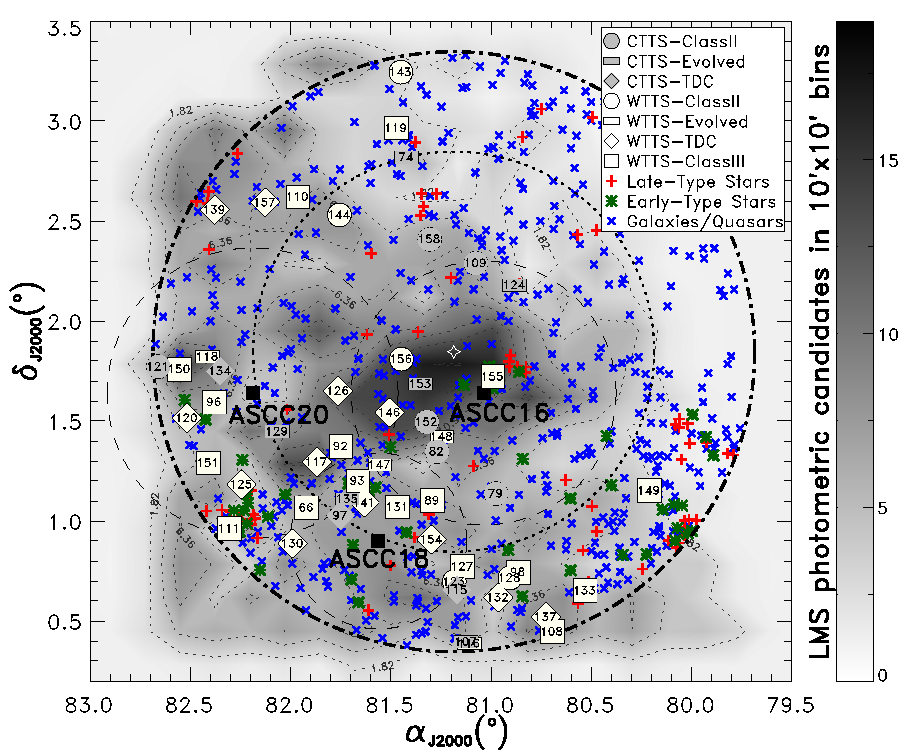
\includegraphics[width=1.\textwidth]{f1.pdf}
	\caption[Spatial distribution of the targets in the 25 Ori BOSS plate]{Spatial distribution of the confirmed members of 25 Ori or Orion OB1a classified as CTTSs and WTTSs on the BOSS plate dedicated to 25 Ori (thick dashed-dotted circle); see Sections \ref{sec_BOSS:memberships} and \ref{sec_BOSS:TTSclass}. The labeled circles, horizontal bars, diamonds, and squares represent YSOs classified as Class II objects, evolved systems, TDC or Class III objects, respectively, as shown in the label box (see Section \ref{sec_BOSS:SED}). The dotted circle represents the estimated area of 25 Ori \citep[1$^\circ$ radius; ][]{Briceno2005,Briceno2007}. The red plus signs, green asterisks, and blue cross signs indicate, respectively, stars later than G spectral type, G-type or earlier stars, and the galaxy/quasar samples. The black filled squares and the dashed circles around them represent, respectively, the central position and estimated area of the labeled stellar groups from \citet{Kharchenko2013}. The gray background map and the labeled isocontours indicate the LMS and BD photometric candidate density in 10'x10' bins from \cite{Downes2014}. The white star sign at the center represents the position of the 25 Orionis star.}
	\label{fig_BOSS:sky}
\end{figure*}

\begin{figure*}[ht!]
	\centering
	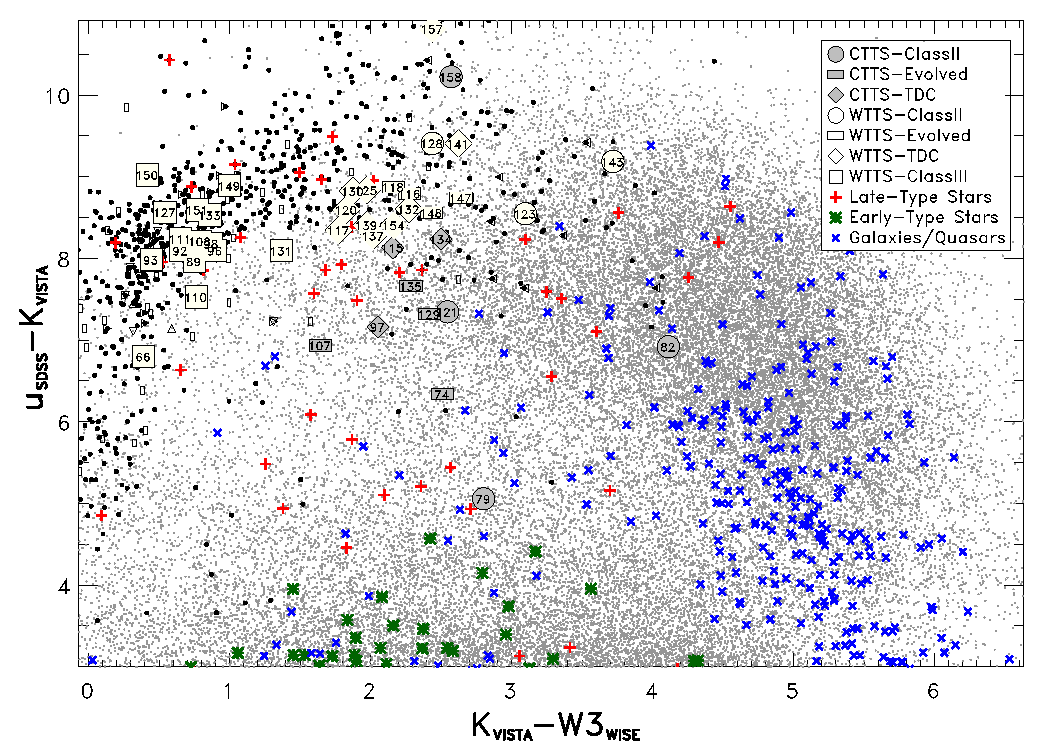
\includegraphics[width=1.\textwidth]{f2.pdf}
	\caption[Color-color diagram of the targets in the 25 Ori BOSS plate]{Color-color diagram showing the targets observed in the 25 Ori BOSS plate. The open upward triangles, downward triangles, rightfacing triangles, leftfacing triangles, and vertical bars indicate, respectively, previously confirmed members by \citet{Briceno2005,  Briceno2007, Downes2014, Downes2015, Briceno2018}. The black points represent the LMS and BD photometric candidates from \citet{Downes2014}, which were selected with an efficiency of $\sim 86\%$ from color-magnitude diagrams where a bias toward sources with IR excesses is not expected. The gray points show the SDSS+VISTA+WISE detections in the 25 Ori BOSS plate field of view. The rest of the symbols are indicated in the label. Note that the gray labeled symbols represent young stars showing intense H$_\alpha$ emission, as explained in Section \ref{sec_BOSS:TTSclass}.}
	\label{fig_BOSS:CCD_bias}
\end{figure*}

The BOSS ancillary science programs made use of the \texttt{v5\_7\_2} version of the \texttt{idlspec2d} pipeline, which, together with \texttt{idlutils}, are the SDSS pipelines used for the data reduction\footnote {\emph{\footnotesize SDSS data processing software is publicly available at \url{http://www.sdss.org/dr12/software/products/}}}. A detailed explanation of the automated classification and the redshift measurements was provided by \citet{Bolton2012}.

The calibrated wavelengths of the BOSS spectra are in the vacuum reference. In order to recognize spectral lines and to use stellar templates to analyze the BOSS spectra, it is needed to convert wavelengths from vacuum to air. We used the IAU standard transformations, as given in \citet{Morton1991}.

\subsubsection{Analysis and Results}
\label{sec_BOSS:results}
In Figure \ref{fig_BOSS:IvsI-J} we show the $I$ vs $I-J$ color-magnitude diagram for all the targets of the 25 Ori BOSS plate, together with the confirmed members in 25 Ori and Orion OB1a from \citet[][]{Briceno2005, Briceno2007, Downes2014, Downes2015}. We also included the 25 Ori members from \citet{Briceno2018}, which were selected according to their position in optical-near-IR color-magnitude diagrams and confirmed on the basis of youth indicators (e.g. H$_\alpha$ emission and NaI$\lambda6708$ absorption) and radial velocities, when available. Additionally, we included the photometric candidates from \citet{Hernandez2007b, Downes2014}. In this diagram, the confirmed members form a very clear locus, nicely separated from the Galactic disk dwarf stars and giant star branches, as well as from extragalactic sources. This shows that the combination of optical and near-IR photometry in color-magnitude diagrams allow for a clear selection of photometric candidates in regions like Orion OB1a \citep[e.g.,][]{Downes2014}.

\begin{figure*}[ht!]
	\centering
	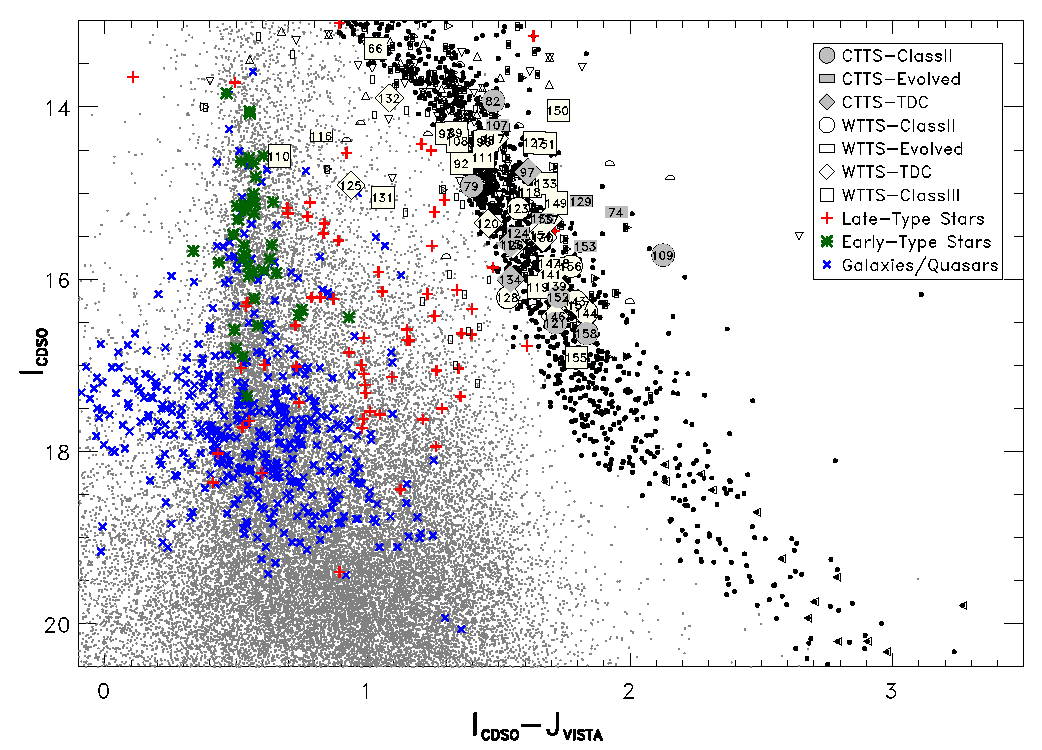
\includegraphics[width=1.\textwidth]{f3.pdf}
	\caption[Color-magnitude diagram of the targets in the 25 Ori BOSS plate]{Color-magnitude diagram from the CDSO and VISTA catalogs. The black points and open small symbols are as in Figure \ref{fig_BOSS:CCD_bias}. The open half circles represent the photometric candidates from \citet{Hernandez2007b}. The gray points show the CDSO+VISTA detections in the 25 Ori BOSS plate field of view. The rest of the symbols are indicated in the label.}
	\label{fig_BOSS:IvsI-J}
\end{figure*}

The BOSS spectra in the DR12 archive are provided with a spectral classification as well as an object classification (star, galaxy or quasar). The stellar templates used for this automated classification are mainly selected from The Indo-US Library \citep{Valdes2004}, which is focused on F- and early G-type stars. The library was supplemented for cool stars by theoretical atmosphere models computed using the MARCS models \citep{Gustafsson2008}. The M-type stellar templates in the database are representative of giant stars with effective temperature down to 3000 K, and a grid resolution of 500 K \citep{Palacios2010}. Thus, these templates are generally not suitable for the spectral type classification of young dwarf stars. Also, the grid resolution in effective temperature of the templates is not enough for the diversity of M-type stars present in our sample. Thus, to determine accurate physical parameters for the BOSS stars (extinction, effective temperature, bolometric luminosity, age, and mass), it is important to verify the SDSS spectral type classification independently. We visually inspected all spectra on the 25 Ori BOSS plate, confirming all objects correctly classified as stars by SDSS, and also identifying those sources for which the SDSS classification was incorrect, either stars classified as galaxies or quasars or, conversely, galaxies or quasars as stars. Through this process, we found 172 stellar spectra out of a total of 677 targets observed on the 25 Ori BOSS plate. The 505 remaining spectra from this plate correspond to either galaxies or quasars, as shown in Figure \ref{fig_BOSS:sky}.

%\floattable
\begin{table*} \scriptsize
 \caption[Photometric catalog of the confirmed members from the BOSS spectra]{Photometric catalog of the confirmed members of 25 Ori or Orion OB1a.}
 \label{tab_BOSS:photometry}
 \begin{threeparttable}
  \setlength{\tabcolsep}{12pt}
  %\renewcommand{\arraystretch}{1.5}
  \begin{tabular}{@{\extracolsep{2pt}}ccccccccccc@{}}
	\toprule
	{\bf ID} & {\bf $\alpha_{J2000}$} & $\delta_{J2000}$ & \multicolumn{5}{c}{{\bf SDSS}} & \multicolumn{3}{c}{{\bf CDSO}} \\
   	\cline{4-8}
   	\cline{9-11}
	& & & $u$ & $g$ & $r$ & $i$ & $z$ & $V$    & $R$    & $I$ \\
	\midrule
 	66  & 81.919314 & 1.065933 & 18.281    & 15.971    & 14.664    & 14.256    & 13.48     & 15.194 & 14.336 & 13.318 \\
  	74  & 81.421671 & 2.818307 & 18.326    & 17.989    & 17.294    & 16.394    & 15.679    & 17.935 & 16.772 & 15.223 \\
  	79  & 80.975436 & 1.136898 & 17.565    & 17.46     & 16.39     & 15.777    & 15.051    & 16.832 & 15.932 & 14.917 \\
  	82  & 81.269534 & 1.347489 & 18.175    & 17.499    & 16.287    & 15.147    & 14.329    & 16.621 & 15.302 & 13.93  \\
  	89  & 81.292164 & 1.102412 & 20.133    & 17.362    & 16.228    & 15.094    & 14.409    & 16.829 & 15.738 & 14.297 \\
  	92  & 81.747728 & 1.373077 & 20.591    & 18.091    & 16.675    & 15.412    & 14.743    & 17.287 & 16.203 & 14.657 \\
  	93  & 81.664785 & 1.200688 & 20.171    & 17.681    & 16.272    & 15.092    & 14.445    & 16.878 & 15.789 & 14.309 \\
  	96  & 82.379687 & 1.594114 & 20.233    & 17.702    & 16.291    & 15.081    & 14.415    & 16.926 & 15.903 & 14.404 \\
  	97  & 81.75054  & 1.026903 & 19.279    & 18.115    & 16.778    & 15.467    & 14.674    & 17.569 & 16.325 & 14.755 \\
  	98  & 80.864815 & 0.743855 & 20.267    & 17.855    & 16.422    & 15.156    & 14.419    & 17.061 & 16.022 & 14.386 \\
	\bottomrule
   \vspace{-1.5ex}
%\tablecomments{The complete version of this table is available in the electronic version of this publication.}
  \end{tabular}
  \setlength{\tabcolsep}{5pt}
  \begin{tabular}{@{\extracolsep{2pt}}p{0.5cm}ccccccccccccccc@{}}
	\toprule
	\multicolumn{5}{c}{{\bf VISTA}} & \multicolumn{3}{c}{{\bf 2MASS}} & \multicolumn{4}{c}{{\bf IRAC}} & \multicolumn{4}{c}{{\bf WISE}} \\
	\cline{1-5}
	\cline{6-8}
	\cline{9-12}
	\cline{13-16}
	$Z$    & $Y$    & $J$    & $H$    & $K$  & $J$ & $H$ & $K$ & CH1 & CH2 & CH3 & CH4 & W1 & W2 & W3 & W4 \\
	\midrule
	13.278     & 12.907     & 12.286     & 11.689     & 11.483     & 12.114     & 11.428     & 11.27      & ...      & ...      & ...      & ...      & 11.242 & 11.183 & 11.092 & 8.305 \\ %& \arrayrulecolor{Gray}\hline
	14.415     & 13.89      & 13.275     & 12.563     & 11.989     & 13.585     & 12.862     & 12.353     & ...      & ...      & ...      & ...      & 11.403 & 10.89  & 9.479  & 7.651 \\ %& \arrayrulecolor{Gray}\hline
	14.628     & 14.094     & 13.519     & 12.941     & 12.507     & 13.5       & 12.757     & 12.295     & ...      & ...      & ...      & ...      & 11.752 & 11.259 & 9.705  & 7.639 \\ %& \arrayrulecolor{Gray}\hline
	13.467     & 12.803     & 12.45      & 11.748     & 11.255     & 12.457     & 11.666     & 11.059     & 10.043   & ...      & 9.22     & ...      & 10.167 & 9.494  & 7.142  & 5.08  \\ %& \arrayrulecolor{Gray}\hline
	13.867     & 13.446     & 12.96      & 12.382     & 12.17      & 12.969     & 12.321     & 12.082     & ...      & ...      & ...      & ...      & 12.001 & 11.861 & 11.42  & 8.552 \\ %& \arrayrulecolor{Gray}\hline
	14.167     & 13.776     & 13.297     & 12.715     & 12.496     & 13.357     & 12.734     & 12.54      & 12.208   & ...      & 12.209   & ...      & 12.35  & 12.216 & 11.843 & 8.279 \\ %& \arrayrulecolor{Gray}\hline
	13.914     & 13.479     & 13.007     & 12.392     & 12.188     & 13.079     & 12.386     & 12.155     & ...      & ...      & ...      & ...      & 12.036 & 11.912 & 11.743 & 8.913 \\ %& \arrayrulecolor{Gray}\hline
	13.906     & 13.444     & 12.957     & 12.374     & 12.138     & 13.02      & 12.355     & 12.109     & ...      & ...      & ...      & ...      & 11.991 & 11.852 & 11.239 & 8.369 \\ %& \arrayrulecolor{Gray}\hline
	14.133     & 13.661     & 13.143     & 12.501     & 12.116     & 13.18      & 12.47      & 12.102     & ...      & ...      & ...      & ...      & 11.587 & 11.176 & 10.062 & 7.028 \\ %& \arrayrulecolor{Gray}\hline
	13.972     & 13.428     & 12.928     & 12.343     & 12.087     & 12.976     & 12.321     & 12.028     & ...      & ...      & ...      & ...      & 11.961 & 11.805 & 11.216 & 8.441 \\ %& \arrayrulecolor{black}
	\bottomrule
  \end{tabular}
  \begin{tablenotes}[para,flushleft]
	(The complete version of this table is available in the electronic version of the \citealt{Suarez2017} publication.) \\
  \end{tablenotes}
 \end{threeparttable}
\end{table*}

\subsubsubsection{Spectral Classification}
\label{sec_BOSS:SpT}
We used the SPTCLASS\footnote {\emph{\footnotesize \url{http://www.cida.gob.ve/~hernandj/SPTclass/sptclass.html}}} semi-automatic code (\citealt{Hernandez2004}; extended to classify the M spectral type regime as published in \citealt{Briceno2005}) to derive spectral types for the 172 stars on the 25 Ori BOSS plate. The code uses empirical relations between the equivalent widths of several effective temperature-sensitive spectral features and the spectral types. Particularly, we are interested in the LMS regime, where the SPTCLASS code uses 10 TiO molecular bands in the wavelength range 4775-7150 \AA\ and six VO molecular bands in the mid part of the spectra from 7460 to 8880 \AA. For the LMSs, the typical uncertainties from our spectral type classification are $\pm 0.7$ spectral sub-classes, while these increase up to $\pm 5$ spectral sub-classes for stars earlier than G-type. In Figure \ref{fig_BOSS:sptclass} we show the residuals between our spectral types using the SPTCLASS code and the spectral types assigned by the SDSS pipeline. Roughly 30\% of the spectra have differences between these two spectral type classifications of more than three spectral sub-classes, especially for the stars with earlier spectral types. There seems to be a trend for stars later than M0, which is due to the fact that most of the M-type stars in our sample are classified as M5 by the SDSS automated classification algorithm. By visually comparing those spectra with the largest spectral type residuals against templates of young and old field stars from \citet{Luhman2000}, \citet{Briceno2002}, \citet{Luhman2003b} \citet{Luhman2004}, and \citet{Kirkpatrick1999}, respectively, we can confirm that our SPTCLASS classification is always more accurate than the SDSS classification. Therefore, for the rest of this work we use the spectral type classification from the SPTCLASS code, which has been extensively used and proven to be accurate and efficient for stars in the spectral type and age ranges considered in this work \citep[e.g.][]{Briceno2007, Hernandez2007b, Downes2014}. This classification covers a spectral type range from A5 to M6, with more than a half of the sample being M-type stars. Spectral types of our confirmed members of 25 Ori or Orion OB1a on the BOSS plate (see Section \ref{sec_BOSS:memberships}) are listed in Table \ref{tab_BOSS:membership}. In Table \ref{tab_BOSS:field_stars} we list the spectral types of all the stars rejected as members on the 25 Ori BOSS plate.

\begin{figure}
	\begin{minipage}{0.60\textwidth}
		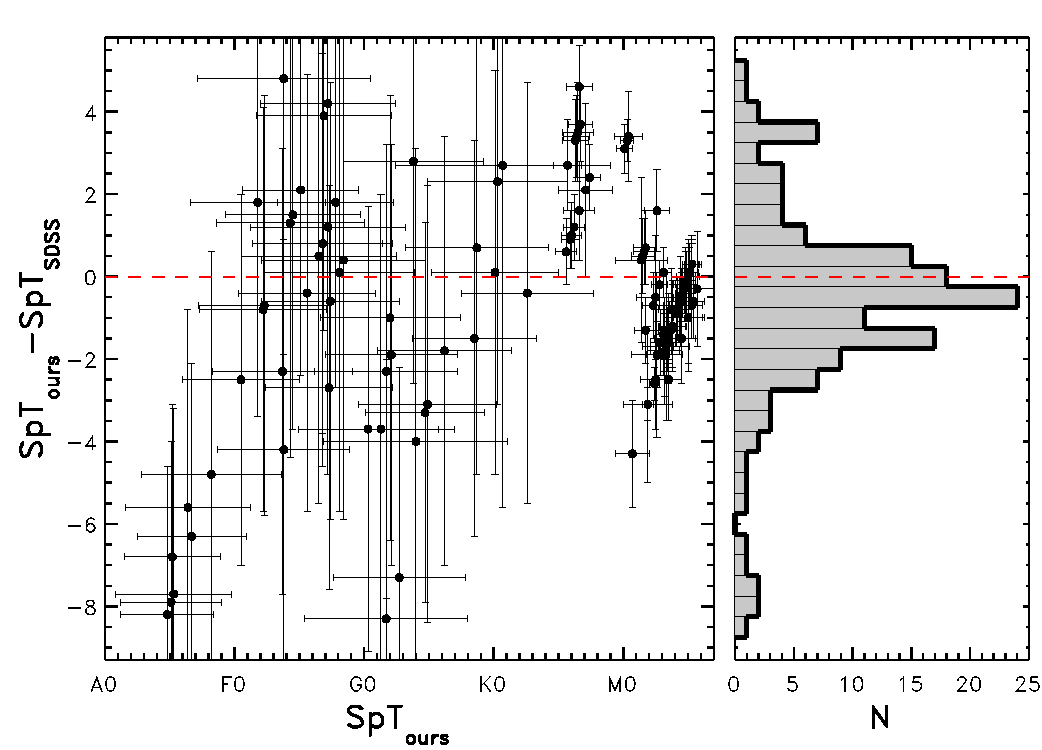
\includegraphics[width=1\textwidth]{f4.pdf}
	\end{minipage} \hfill
	\begin{minipage}{0.35\textwidth}
		\caption[SpT residuals between our classification and that from SDSS]{Residuals between our spectral type classification using the SPTCLASS code \citep{Hernandez2004} and the spectral type assigned by the SDSS pipeline. The associated errors are those estimated by the SPTCLASS code because the SDSS classification does not report spectral type uncertainties. The residuals are given in units of spectral sub-classes.}
		\label{fig_BOSS:sptclass}
	\end{minipage}
\end{figure}

\subsubsubsection{Membership Determination for 25 Ori and Orion OB1a}
\label{sec_BOSS:memberships}

Once the spectral type was determined for all the stars on the 25 Ori BOSS plate, several diagnoses were applied to determine their memberships, depending on their spectral types.

\paragraph{M-type Stars\\}
\label{sec_BOSS:M_stars}

The following criteria were used to assign the 25 Ori and Orion OB1a memberships of the M-type stars:

\begin{itemize}
	\item H$_\alpha$ emission.
				
		The detection of strong H$_\alpha$ emission in young LMSs is due to both the chromospheric activity and accretion phenomena that produce narrow symmetric and broader asymmetric H$_\alpha$ line profiles \citep{Muzerolle2005}, respectively. We considered as possible M-type members those stars showing H$_\alpha$ emission. However, because at the age of 25 Ori most of the accreting circumstellar disks have dissipated \citep{Calvet2005}, not only those sources having strong emissions related to accretion are necessary members. Thus, additional criteria are needed to support the memberships of those objects showing weak H$_\alpha$ emission.

	\item LiI$\lambda$6708 absorption.

		For LMSs, the LiI$\lambda$6708 absorption is a well-known indicator of youth \citep{Strom1989, Briceno1998}. It is present in the stellar surface of LMSs because they are fully convective in the PMS phase and the mixing timescale is shorter than the time they need to reach the MS \citep{Soderblom1993}. Therefore, we used the presence of the LiI$\lambda$6708 absorption as an additional membership criterion for the LMSs.

	\item Weak NaI$\lambda\lambda$8183, 8195 doublet in absorption relative to a field star of the same spectral type.

		An additional youth indicator for the M-type stars is the NaI$\lambda\lambda$8183,8195 doublet in absorption, which is sensitive to surface gravity. Since the PMS stars are still contracting, they have lower surface gravity than MS stars with the same spectral type, such that the NaI$\lambda\lambda$8183, 8195 doublet is measurably weaker in PMS sources \citep{Luhman2003a}. We compared the BOSS M-type spectra with templates for young and old field stars with the same spectral type from, respectively, \citet{Luhman2000}, \citet{Briceno2002}, \citet{Luhman2003b} and \citet{Luhman2004}, and \citet{Kirkpatrick1999}, to determine if the NaI$\lambda\lambda$8183,8195 doublet is consistent with the weak absorption expected for a bona fide young star.

\end{itemize}

Summarizing these criteria, we confirm a M-type star as a 25 Ori or Orion OB1a member if it exhibits any level of H$_\alpha$ emission and either LiI$\lambda$6708 absorption or NaI$\lambda\lambda$8183, 8195 absorption whose profile agrees with a young stellar template of the same spectral type. Based on these criteria, we confirmed a total of 53 members of 25 Ori or Orion OB1a with spectral types from M0 to M6. Three of these members (148, 153, and 156) have already been confirmed as young members by \citet{Downes2014}, so we can report the finding of a total of 50 new confirmed members of 25 Ori or Orion OB1a. In Table \ref{tab_BOSS:membership} we summarize the membership criteria for these confirmed members. About 87\% of the M-type confirmed members have LiI$\lambda$6708 absorption equivalent widths W(LiI)$>$0.15 \AA\ and the rest have a clear weak NaI$\lambda\lambda$8183, 8195 doublet. The 81\% of the members have the NaI$\lambda\lambda$8183, 8195 doublet in absorption consistent with the young stellar templates and for most of the remaining members the NaI$\lambda\lambda$8183, 8195 is not conclusive but they show a clear LiI$\lambda$6708 absorption. As an example, in Figure \ref{fig_BOSS:membership} we show the spectrum of the member 157 with enlargements of the H$_\alpha$ emission, LiI$\lambda$6708 absorption and weak NaI$\lambda\lambda$8183, 8195 absorption youth indicators we used to assign its membership.

The 50 new confirmed members represent an increase of $\approx 30\%$ the number of known sub-solar members of 25 Ori or Orion OB1a in the region covered by the considered BOSS plate \citep{Briceno2005,Briceno2007,Hernandez2007b,Downes2014,Downes2015}. Of these members, 22 are inside the \citet{Briceno2005,Briceno2007} estimated area of 25 Ori (1$^\circ$ radius), which represents an increase of $\approx 14\%$ in the number of 25 Ori confirmed members in the sub-solar mass range. Throughout this study, we conservatively worked with the 25 Ori estimated radius of 1$^\circ$, which is greater than the 0.5$^\circ$ radius of the 25 Ori overdensity estimated by \citet{Downes2014}.

\paragraph{K-type Stars\\}
\label{sec_BOSS:K_stars}

The H$_\alpha$ emission and LiI$\lambda$6708 absorption membership criteria discussed in Section \ref{sec_BOSS:M_stars} also apply for the K-type stars. Therefore, K-type stars were selected as YSOs when presenting H$_\alpha$ emission and LiI$\lambda$6708 absorption. From the 20 K-type stars in the BOSS stellar spectra, we did not confirm any K-type member. None present both LiI$\lambda$6708 absorption and H$_\alpha$ emission (only two stars have weak H$_\alpha$ emission, but those lack LiI$\lambda$6708 absorption).

\paragraph{Early-type Stars\\}
\label{sec_BOSS:early_stars}

The membership criteria discussed in Section \ref{sec_BOSS:M_stars} cannot be applied to stars earlier than K-type (43 stars of the sample). In fact, there is not a clear way to confirm these stars as young members with the available information. We checked the position of these stars in the $I$ vs $I-J$ color-magnitude diagram. We found that not a single early-type star lies within the 25 Ori locus, even when considering the effects of variability. The position of these stars is consistent with the field stars.

The most robust membership diagnostic for stars earlier than K spectral type is their kinematics, though X-ray emission, IR excesses or variability are useful secondary indicators. The spectral resolution of BOSS is not high enough to provide precise radial velocities to determine kinematic memberships for these early type stars, so we checked the other criteria. None of these stars have X-ray counterparts in the 3XMM-DR5 database \citep{Rosen2016} or in the Chandra Source Catalog \citep{Evans2010}. Additionally, none of these stars are high-probability variable stars according to the CVSO catalog or have IR excesses according to the photometric selection from \citet{Cottle2018}, based on 2MASS+WISE photometry and the algorithm developed by \citet{Koenig2014}. Therefore, the stars earlier than K spectral type on the 25 Ori BOSS plate are likely non-members.

\begin{table} \scriptsize
 \caption[Youth indicators of the confirmed members from the BOSS spectra]{Confirmed members and their youth indicators.}
 \label{tab_BOSS:membership}
 \begin{threeparttable}
  \setlength{\tabcolsep}{10pt}
  \renewcommand{\arraystretch}{1.034}
	\begin{minipage}{0.48\textwidth}
	  \begin{tabular}{ccccc}
		\toprule
		{\bf ID} & {\bf SpT} & {\bf WH$_\alpha$} & {\bf WLiI$\lambda6708$} & {\bf NaI} \\
		   &     & (\AA)       & (\AA)             &     \\
		\midrule
		66  & M0.3$\pm$0.5  & -2.062  & 0.4257  & 0   \\ 
	  	74  & M1.5$\pm$1.2  & -161.8  & 0.2514  & -1  \\ 
	  	79  & M1.9$\pm$0.4  & -247.7  & 0.3037  & 1   \\ 
	  	82  & M2.4$\pm$0.4  & -52.95  & 0.2569  & 1   \\ 
	  	89  & M2.8$\pm$0.6  & -5.843  & 0.1607  & 1   \\ 
	  	92  & M3.1$\pm$0.5  & -4.39   & ---     & 1   \\ 
	  	93  & M3.1$\pm$0.5  & -3.541  & 0.1659  & 1   \\ 
	  	96  & M3.2$\pm$0.5  & -4.448  & 0.3134  & 1   \\ 
	  	97  & M3.2$\pm$0.5  & -38.64  & 0.446   & 1   \\ 
	  	98  & M3.2$\pm$0.6  & -5.865  & 0.4586  & 1   \\ 
	  	107 & M3.5$\pm$0.5  & -39.31  & 0.2887  & 1   \\ 
	  	108 & M3.5$\pm$0.6  & -7.876  & ---     & 1   \\ 
	  	109 & M3.5$\pm$1.0  & -41.43  & 0.577   & 0   \\ 
	  	110 & M3.5$\pm$1.1  & -7.721  & 0.2379  & 1   \\ 
	  	111 & M3.7$\pm$0.6  & -4.347  & 0.4181  & 1   \\ 
	  	115 & M4.1$\pm$0.7  & -16.54  & 0.4601  & 1   \\ 
	  	116 & M4.1$\pm$0.7  & -6.188  & 0.4777  & 1   \\ 
	  	117 & M4.2$\pm$0.7  & -6.016  & 0.3093  & 1   \\ 
	  	118 & M4.3$\pm$0.7  & -9.375  & 0.412   & 1   \\ 
	  	119 & M4.4$\pm$1.1  & -14.06  & 0.3332  & -1  \\ 
	  	120 & M4.5$\pm$0.7  & -5.663  & ---     & 1   \\ 
	  	121 & M4.5$\pm$0.7  & -62.18  & 0.0799  & 1   \\ 
	  	123 & M4.5$\pm$0.6  & -6.398  & 0.5469  & 1   \\ 
	  	124 & M4.5$\pm$1.1  & -47.26  & 0.6343  & -1  \\ 
	  	125 & M4.6$\pm$0.6  & -7.454  & ---     & 1   \\ 
	  	126 & M4.6$\pm$0.6  & -8.915  & 0.3241  & 1   \\ 
	  	127 & M4.6$\pm$0.5  & -10.15  & 0.3781  & 0   \\ 
	  	128 & M4.6$\pm$0.5  & -3.17   & 0.5076  & 1   \\ 
		\bottomrule
	  \end{tabular}
	\end{minipage} \hfill
	\begin{minipage}{0.48\textwidth}
  	\setlength{\tabcolsep}{10pt}
	\renewcommand{\arraystretch}{1.0}
	  \begin{tabular}{ccccc}
		\toprule
		{\bf ID} & {\bf SpT} & {\bf WH$_\alpha$} & {\bf WLiI$\lambda6708$} & {\bf NaI} \\
		   &     & (\AA)       & (\AA)             &     \\
		\midrule
	  	129 & M4.7$\pm$0.5  & -74.23  & 0.2364  & 1   \\ 
	  	130 & M4.7$\pm$0.5  & -6.109  & 0.5821  & 1   \\ 
	  	131 & M4.7$\pm$0.5  & -4.569  & 0.5341  & 1   \\ 
	  	132 & M4.7$\pm$0.4  & -12.02  & 0.5568  & 1   \\ 
	  	133 & M4.7$\pm$0.5  & -12.18  & 0.3165  & 1   \\ 
	  	134 & M4.8$\pm$0.4  & -21.34  & 0.1725  & 1   \\ 
	  	135 & M4.8$\pm$0.5  & -59.07  & 0.4103  & 1   \\ 
	  	137 & M4.8$\pm$0.5  & -10.11  & 0.5883  & 1   \\ 
	  	139 & M4.8$\pm$0.9  & -14.6   & ---     & 1   \\ 
	  	141 & M5.0$\pm$0.6  & -9.543  & 0.5009  & 1   \\ 
	  	143 & M5.0$\pm$1.3  & -14.41  & 0.8292  & -1  \\ 
	  	144 & M5.0$\pm$1.1  & -14.36  & 0.8965  & 1   \\ 
	  	146 & M5.1$\pm$0.6  & -15.92  & 0.7128  & 1   \\ 
	  	147 & M5.1$\pm$0.6  & -12.69  & 0.6626  & 1   \\ 
	  	148 & M5.1$\pm$0.7  & -8.659  & 0.6687  & 1   \\ 
	  	149 & M5.1$\pm$0.7  & -11.33  & 0.593   & 1   \\ 
	  	150 & M5.3$\pm$0.6  & -13.43  & 0.354   & 0   \\ 
	  	151 & M5.3$\pm$0.5  & -14.57  & 0.3275  & 1   \\ 
	  	152 & M5.3$\pm$0.7  & -88.18  & 0.5188  & 1   \\ 
	  	153 & M5.3$\pm$0.6  & -32.65  & 0.534   & 1   \\ 
	  	154 & M5.3$\pm$0.6  & -12.34  & 0.7089  & 1   \\ 
	  	155 & M5.3$\pm$0.7  & -14.95  & 1.056   & 0   \\ 
	  	156 & M5.3$\pm$0.8  & -12.88  & ---     & 1   \\ 
	  	157 & M5.4$\pm$0.9  & -7.491  & 0.6515  & 1   \\ 
	  	158 & M5.7$\pm$1.4  & -29.84  & 1.712   & 0   \\ 
		\bottomrule
	  \end{tabular}
	  \begin{tablenotes}[para,flushleft]
	    For the NaI$\lambda\lambda$8183, 8195 absorption, the 1, -1, and 0 flags mean, respectively, if the feature is consistent with a young stellar template, an old stellar template or not conclusive.\\
	  \end{tablenotes}
	\end{minipage}
 \end{threeparttable}
\end{table}

\begin{figure*}%[H]
	\centering 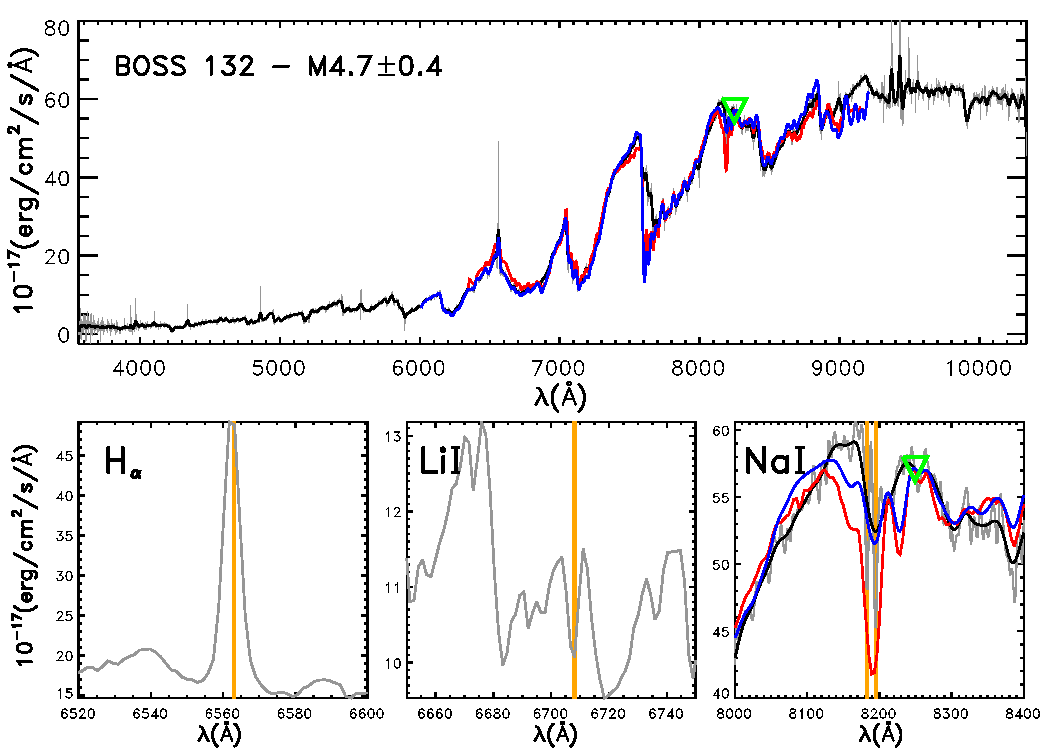
\includegraphics[width=1.\textwidth]{f5.pdf}
	\caption[Membership criteria for M-type stars]{Example of one of the confirmed LMS members in Orion OB1a (member 132 from Table \ref{tab_BOSS:membership}). \textbf {Upper panel:} BOSS spectrum with the original resolution of 1.4 \AA\ (gray solid line) and with a convolved resolution of 16 \AA\ (black solid line). The stellar templates with the same spectral type as this confirmed member are shown with a resolution of 16 \AA\ for a field star from \citet{Kirkpatrick1999} (red line) and for a young star from the lists by \citet{Luhman2000,Briceno2002,Luhman2003b} and \citet{Luhman2004} (blue line). The green triangle indicates the normalization point of the stellar templates' fluxes, which is located in the pseudo-continuum of the NaI$\lambda\lambda$8183, 8195 doublet of the BOSS spectrum \citep{Schlieder2012}. \textbf {Lower panel:} Enlargements of the H$_\alpha$ emission, LiI$\lambda$6708 absorption and weak NaI$\lambda\lambda$8183, 8195 doublet youth indicators used to assign the memberships of the LMSs. The orange vertical solid lines show the wavelength range of the indicated features. For member 132, the spectrum presents H$_\alpha$ emission, LiI$\lambda$6708 absorption and the NaI$\lambda\lambda$8183, 8195 doublet consistent with the young stellar template. Therefore, this star was confirmed as a young LMS member.}
	\label{fig_BOSS:membership}
\end{figure*}

\subsubsubsection{Physical Parameters}
\label{sec_BOSS:parameters}

As described in \citet{Luhman1999}, the $I$ and $J$ bands are preferred to estimate bolometric luminosities of young LMSs because the contamination from UV and IR excess emission is minimal. We used the $I$ band from the CDSO and the $J$ band from VISTA to determine the extinction and bolometric luminosity of our confirmed members.

\paragraph{Extinctions\\}
\label{sec_BOSS:extinction}
The visual extinction ($A_V$) toward each confirmed member was calculated using the observed $I-J$ color, an assumed intrinsic $I-J$ color for a young star of the same measured spectral type and the extinction law from \citet{Fitzpatrick1999}, assuming $R_V=3.1$. The adopted intrinsic $I-J$ color was obtained by interpolating the spectral type in the empirical relations from \citet{Kenyon-Hartmann1995}, \citet{Luhman1999}, \citet{Briceno2002}, and \citet{Luhman2003a}. These relationships were designed to match the \citet{Baraffe1998} tracks, as explained by \citet{Luhman2003b}.

In Table \ref{tab_BOSS:parameters} we list the extinctions we estimated toward each confirmed LMS member of 25 Ori or Orion OB1a. Removing the two members having the highest unexpected extinctions (member 74 and 109 with $A_V=4.33^{+0.51}_{-0.98}$ and $A_V=3.53^{+0.94}_{-1.01.}$ mag, respectively), we obtained a mean extinction $\bar{A}_V$=0.14 mag and a standard deviation $\sigma _{A_V}=0.31$ mag toward the complete sample of confirmed members in 25 Ori and Orion OB1a, which is agreement with the mean extinction $\bar{A}_V$=0.16 mag, obtained by \citet{Downes2015}. If we only consider the confirmed members inside the 25 Ori's estimated area, we obtain $\bar{A}_V$=0.21 mag and $\sigma _{A_V}=0.43$ mag, which is also in agreement with previous extinction estimates in 25 Ori \citep[0.27 mag, 0.28 mag, 0.29 mag, and 0.30 mag by ][respectively]{Kharchenko2005, Briceno2005, Briceno2007, Downes2014}.

\begin{table} \scriptsize
 \caption[Physical parameters of the confirmed members using BOSS spectra]{Physical parameters of the 53 confirmed members.}
 \label{tab_BOSS:parameters}
 \begin{threeparttable}
  	\setlength{\tabcolsep}{5pt}
	\begin{tabular}{lclclclclclccc}
	\toprule
	{\bf ID} & {\bf $A_\textrm{v}$} & {\bf e\_$A_\textrm{v}$} &  {\bf T$_{eff}$}   & {\bf e\_T$_{eff}$}  & {\bf L}           & {\bf e\_L}          & {\bf $m$}         & {\bf e\_$m$}        & {\bf age}   & {\bf e\_age} & {\bf TTS} & {\bf Disk Type} & {\bf Location} \\
	   & (mag.)         & (mag.)          & (K)  & (K) & (L$_\odot$) & (L$_\odot$) & (M$_\odot$) & (M$_\odot$) & (Myr) & (Myr)              &     &           & \\
	\midrule
 	66$^a  $    & 0.193 & $^{+0.325}_{-0.203}$ & 3806.5 & $^{+85.5  }_{-72.5 }$ & 0.286 & $^{+0.125 }_{-0.118}$ & 0.573 & $^{+0.038 }_{-0.073}$ & 4.175  & $^{+10.597 }_{-2.387}$  & WTTS & ClassIII & ASCC18/ASCC20 \\
 	74          & 4.33  & $^{+0.513}_{-0.975}$ & 3632.5 & $^{+174.0 }_{-174.0}$ & 0.312 & $^{+0.195 }_{-0.221}$ & 0.425 & $^{+0.101 }_{-0.125}$ & 2.026  & $^{+12.817 }_{-1.338}$  & CTTS & Evolved  & Outside       \\
 	79$^a  $    & 1.355 & $^{+0.183}_{-0.366}$ & 3574.5 & $^{+58.0  }_{-58.0 }$ & 0.111 & $^{+0.028 }_{-0.031}$ & 0.445 & $^{+0.036 }_{-0.045}$ & 8.959  & $^{+5.93   }_{-3.864}$  & CTTS & ClassII  & 25Ori         \\
 	82$^a  $    & 1.299 & $^{+0.426}_{-0.426}$ & 3502.0 & $^{+58.0  }_{-58.0 }$ & 0.276 & $^{+0.09  }_{-0.09 }$ & 0.353 & $^{+0.016 }_{-0.052}$ & 1.79   & $^{+1.686  }_{-0.853}$  & CTTS & ClassII  & 25Ori         \\
 	89$^a  $    & 0.147 & $^{+0.64 }_{-0.538}$ & 3444.0 & $^{+87.0  }_{-87.0 }$ & 0.126 & $^{+0.087 }_{-0.08 }$ & 0.331 & $^{+0.047 }_{-0.031}$ & 4.189  & $^{+10.642 }_{-2.699}$  & WTTS & ClassIII & 25Ori/ASCC18  \\
 	92          & 0.0   & $^{+0.508}_{-0.0  }$ & 3400.5 & $^{+72.5  }_{-72.5 }$ & 0.081 & $^{+0.036 }_{-0.029}$ & 0.306 & $^{+0.053 }_{-0.024}$ & 6.79   & $^{+8.043  }_{-3.529}$  & WTTS & ClassIII & ASCC20        \\
 	93$^a  $    & 0.0   & $^{+0.508}_{-0.0  }$ & 3400.5 & $^{+72.5  }_{-72.5 }$ & 0.117 & $^{+0.074 }_{-0.061}$ & 0.3   & $^{+0.047 }_{-0.019}$ & 3.808  & $^{+11.07  }_{-2.231}$  & WTTS & ClassIII & ASCC18/ASCC20 \\
 	96$^a  $    & 0.33  & $^{+0.482}_{-0.406}$ & 3386.0 & $^{+72.5  }_{-72.5 }$ & 0.119 & $^{+0.052 }_{-0.049}$ & 0.299 & $^{+0.035 }_{-0.034}$ & 3.704  & $^{+7.801  }_{-1.933}$  & WTTS & ClassIII & ASCC20        \\
 	97$^a  $    & 1.168 & $^{+0.482}_{-0.406}$ & 3386.0 & $^{+72.5  }_{-72.5 }$ & 0.139 & $^{+0.062 }_{-0.058}$ & 0.296 & $^{+0.034 }_{-0.031}$ & 2.977  & $^{+6.142  }_{-1.566}$  & CTTS & TDC      & ASCC18        \\
 	98$^a  $    & 0.386 & $^{+0.589}_{-0.487}$ & 3386.0 & $^{+87.0  }_{-87.0 }$ & 0.13  & $^{+0.077 }_{-0.073}$ & 0.297 & $^{+0.047 }_{-0.051}$ & 3.271  & $^{+11.597 }_{-1.978}$  & WTTS & ClassIII & Outside       \\
 	107$^a $    & 0.33  & $^{+0.406}_{-0.406}$ & 3342.5 & $^{+72.5  }_{-72.5 }$ & 0.156 & $^{+0.082 }_{-0.082}$ & 0.272 & $^{+0.028 }_{-0.058}$ & 2.208  & $^{+6.233  }_{-1.237}$  & CTTS & Evolved  & Outside       \\
 	108         & 0.0   & $^{+0.513}_{-0.0  }$ & 3342.5 & $^{+87.0  }_{-87.0 }$ & 0.113 & $^{+0.066 }_{-0.06 }$ & 0.278 & $^{+0.025 }_{-0.076}$ & 3.513  & $^{+11.273 }_{-2.028}$  & WTTS & ClassIII & Outside       \\
 	109         & 3.533 & $^{+0.939}_{-1.066}$ & 3342.5 & $^{+145.0 }_{-145.0}$ & 0.157 & $^{+0.118 }_{-0.118}$ & 0.271 & $^{+0.075 }_{-0.071}$ & 2.188  & $^{+12.64  }_{-1.683}$  & CTTS & ClassII  & 25Ori         \\
 	110         & 0.0   & $^{+1.046}_{-0.0  }$ & 3342.5 & $^{+159.5 }_{-159.5}$ & 0.096 & $^{+0.086 }_{-0.069}$ & 0.282 & $^{+0.088 }_{-0.084}$ & 4.537  & $^{+10.338 }_{-3.771}$  & WTTS & ClassIII & Outside       \\
 	111         & 0.0   & $^{+0.487}_{-0.0  }$ & 3313.5 & $^{+87.0  }_{-87.0 }$ & 0.093 & $^{+0.046 }_{-0.04 }$ & 0.263 & $^{+0.037 }_{-0.063}$ & 4.353  & $^{+8.988  }_{-2.617}$  & WTTS & ClassIII & ASCC20        \\
 	115$^a $    & 0.046 & $^{+0.62 }_{-0.924}$ & 3255.5 & $^{+101.5 }_{-101.5}$ & 0.042 & $^{+0.027 }_{-0.029}$ & 0.207 & $^{+0.088 }_{-0.028}$ & 8.578  & $^{+6.298  }_{-5.968}$  & CTTS & TDC      & Outside       \\
 	116         & 0.0   & $^{+0.619}_{-0.0  }$ & 3255.5 & $^{+101.5 }_{-101.5}$ & 0.13  & $^{+0.083 }_{-0.074}$ & 0.218 & $^{+0.054 }_{-0.039}$ & 2.19   & $^{+8.071  }_{-1.685}$  & WTTS & Evolved  & Outside       \\
 	117         & 0.0   & $^{+0.67 }_{-0.0  }$ & 3241.0 & $^{+101.5 }_{-101.5}$ & 0.122 & $^{+0.07  }_{-0.058}$ & 0.206 & $^{+0.062 }_{-0.04 }$ & 2.204  & $^{+5.67   }_{-1.606}$  & WTTS & TDC      & ASCC20        \\
 	118$^a $    & 0.162 & $^{+0.721}_{-0.924}$ & 3226.5 & $^{+101.5 }_{-101.5}$ & 0.076 & $^{+0.044 }_{-0.047}$ & 0.2   & $^{+0.07  }_{-0.049}$ & 3.528  & $^{+11.281 }_{-2.451}$  & WTTS & Evolved  & ASCC20        \\
 	119         & 0.188 & $^{+1.097}_{-1.401}$ & 3212.0 & $^{+159.5 }_{-154.5}$ & 0.029 & $^{+0.028 }_{-0.03 }$ & 0.185 & $^{+0.115 }_{-0.085}$ & 10.461 & $^{+---    }_{-8.376}$  & WTTS & ClassIII & Outside       \\
 	120         & 0.0   & $^{+0.822}_{-0.0  }$ & 3197.5 & $^{+101.5 }_{-99.5 }$ & 0.052 & $^{+0.032 }_{-0.026}$ & 0.192 & $^{+0.058 }_{-0.067}$ & 4.924  & $^{+9.879  }_{-3.435}$  & WTTS & TDC      & ASCC20        \\
 	121$^a $    & 0.391 & $^{+0.823}_{-0.904}$ & 3197.5 & $^{+101.5 }_{-99.5 }$ & 0.021 & $^{+0.013 }_{-0.014}$ & 0.173 & $^{+0.067 }_{-0.048}$ & 14.128 & $^{+0.742  }_{-9.579}$  & CTTS & ClassII  & ASCC20        \\
 	123$^a $    & 0.0   & $^{+0.741}_{-0.0  }$ & 3197.5 & $^{+87.0  }_{-86.0 }$ & 0.068 & $^{+0.038 }_{-0.03 }$ & 0.198 & $^{+0.042 }_{-0.06 }$ & 3.635  & $^{+7.512  }_{-2.437}$  & WTTS & ClassII  & ASCC18        \\
 	124         & 0.0   & $^{+1.147}_{-0.0  }$ & 3197.5 & $^{+159.5 }_{-153.5}$ & 0.049 & $^{+0.044 }_{-0.037}$ & 0.191 & $^{+0.099 }_{-0.091}$ & 5.272  & $^{+9.602  }_{-4.006}$  & CTTS & Evolved  & 25Ori         \\
 	125         & 0.0   & $^{+0.792}_{-0.0  }$ & 3183.0 & $^{+87.0  }_{-85.0 }$ & 0.079 & $^{+0.045 }_{-0.036}$ & 0.192 & $^{+0.038 }_{-0.066}$ & 2.755  & $^{+6.192  }_{-1.742}$  & WTTS & TDC      & ASCC20        \\
 	126         & 0.0   & $^{+0.792}_{-0.0  }$ & 3183.0 & $^{+87.0  }_{-85.0 }$ & 0.042 & $^{+0.024 }_{-0.019}$ & 0.182 & $^{+0.042 }_{-0.056}$ & 5.805  & $^{+8.994  }_{-3.891}$  & WTTS & TDC      & ASCC20        \\
 	127$^a $    & 0.0   & $^{+0.66 }_{-0.0  }$ & 3183.0 & $^{+72.5  }_{-71.5 }$ & 0.14  & $^{+0.069 }_{-0.056}$ & 0.183 & $^{+0.039 }_{-0.045}$ & 1.118  & $^{+2.595  }_{-0.612}$  & WTTS & ClassIII & ASCC18        \\
 	128         & 0.0   & $^{+0.66 }_{-0.0  }$ & 3183.0 & $^{+72.5  }_{-71.5 }$ & 0.025 & $^{+0.014 }_{-0.013}$ & 0.171 & $^{+0.036 }_{-0.033}$ & 10.55  & $^{+4.332  }_{-6.362}$  & WTTS & ClassII  & Outside       \\
 	129$^a $    & 0.619 & $^{+0.66 }_{-0.64 }$ & 3168.5 & $^{+72.5  }_{-70.5 }$ & 0.09  & $^{+0.044 }_{-0.044}$ & 0.178 & $^{+0.028 }_{-0.053}$ & 1.966  & $^{+5.167  }_{-1.028}$  & CTTS & Evolved  & ASCC20        \\
 	130$^a $    & 0.0   & $^{+0.66 }_{-0.0  }$ & 3168.5 & $^{+72.5  }_{-70.5 }$ & 0.052 & $^{+0.026 }_{-0.021}$ & 0.18  & $^{+0.021 }_{-0.055}$ & 4.194  & $^{+7.27   }_{-2.586}$  & WTTS & TDC      & ASCC18        \\
 	131         & 0.0   & $^{+0.66 }_{-0.0  }$ & 3168.5 & $^{+72.5  }_{-70.5 }$ & 0.08  & $^{+0.04  }_{-0.033}$ & 0.18  & $^{+0.026 }_{-0.055}$ & 2.371  & $^{+4.579  }_{-1.325}$  & WTTS & ClassIII & ASCC18        \\
 	132$^a $    & 0.0   & $^{+0.528}_{-0.0  }$ & 3168.5 & $^{+58.0  }_{-57.0 }$ & 0.215 & $^{+0.112 }_{-0.1  }$ & 0.181 & $^{+0.019 }_{-0.043}$ & 0.623  & $^{+1.55   }_{-0.116}$  & WTTS & TDC      & Outside       \\
 	133         & 0.0   & $^{+0.66 }_{-0.0  }$ & 3168.5 & $^{+72.5  }_{-70.5 }$ & 0.087 & $^{+0.05  }_{-0.044}$ & 0.179 & $^{+0.028 }_{-0.053}$ & 2.075  & $^{+5.654  }_{-1.17 }$  & WTTS & ClassIII & Outside       \\
 	134         & 0.0   & $^{+0.528}_{-0.0  }$ & 3154.0 & $^{+58.0  }_{-56.0 }$ & 0.03  & $^{+0.013 }_{-0.011}$ & 0.163 & $^{+0.031 }_{-0.037}$ & 7.27   & $^{+7.53   }_{-4.032}$  & CTTS & TDC      & ASCC20        \\
 	135         & 0.0   & $^{+0.66 }_{-0.0  }$ & 3154.0 & $^{+72.5  }_{-69.5 }$ & 0.061 & $^{+0.044 }_{-0.036}$ & 0.173 & $^{+0.027 }_{-0.058}$ & 3.113  & $^{+10.263 }_{-1.943}$  & CTTS & Evolved  & ASCC18/ASCC20 \\
 	137         & 0.0   & $^{+0.66 }_{-0.0  }$ & 3154.0 & $^{+72.5  }_{-69.5 }$ & 0.06  & $^{+0.035 }_{-0.031}$ & 0.173 & $^{+0.027 }_{-0.058}$ & 3.222  & $^{+8.17   }_{-1.924}$  & WTTS & TDC      & Outside       \\
 	139         & 0.005 & $^{+1.137}_{-1.117}$ & 3154.0 & $^{+130.5 }_{-123.5}$ & 0.03  & $^{+0.026 }_{-0.026}$ & 0.163 & $^{+0.071 }_{-0.064}$ & 7.27   & $^{+7.593  }_{-5.211}$  & WTTS & TDC      & Outside       \\
 	141         & 0.0   & $^{+0.792}_{-0.0  }$ & 3125.0 & $^{+87.0  }_{-81.0 }$ & 0.037 & $^{+0.022 }_{-0.019}$ & 0.152 & $^{+0.048 }_{-0.052}$ & 4.762  & $^{+10.03  }_{-2.779}$  & WTTS & TDC      & ASCC18        \\
 	143         & 0.112 & $^{+1.564}_{-1.873}$ & 3125.0 & $^{+188.5 }_{-168.0}$ & 0.027 & $^{+0.035 }_{-0.037}$ & 0.149 & $^{+0.11  }_{-0.069}$ & 6.993  & $^{+---    }_{-5.394}$  & WTTS & ClassII  & Outside       \\
 	144         & 0.33  & $^{+1.401}_{-1.437}$ & 3125.0 & $^{+159.5 }_{-146.0}$ & 0.026 & $^{+0.029 }_{-0.029}$ & 0.148 & $^{+0.086 }_{-0.066}$ & 7.309  & $^{+---    }_{-5.331}$  & WTTS & ClassII  & Outside       \\
 	146         & 0.0   & $^{+0.782}_{-0.0  }$ & 3111.5 & $^{+86.0  }_{-81.0 }$ & 0.021 & $^{+0.018 }_{-0.016}$ & 0.139 & $^{+0.048 }_{-0.04 }$ & 8.428  & $^{+6.447  }_{-5.537}$  & WTTS & TDC      & 25Ori/ASCC20  \\
 	147         & 0.0   & $^{+0.782}_{-0.0  }$ & 3111.5 & $^{+86.0  }_{-81.0 }$ & 0.041 & $^{+0.034 }_{-0.029}$ & 0.146 & $^{+0.054 }_{-0.047}$ & 3.998  & $^{+10.89  }_{-2.444}$  & WTTS & Evolved  & 25Ori/ASCC18  \\
 	148         & 0.0   & $^{+0.914}_{-0.0  }$ & 3111.5 & $^{+100.5 }_{-94.5 }$ & 0.039 & $^{+0.026 }_{-0.022}$ & 0.146 & $^{+0.054 }_{-0.056}$ & 4.187  & $^{+10.589 }_{-2.437}$  & WTTS & Evolved  & 25Ori         \\
 	149         & 0.0   & $^{+0.914}_{-0.0  }$ & 3111.5 & $^{+100.5 }_{-94.5 }$ & 0.075 & $^{+0.056 }_{-0.049}$ & 0.145 & $^{+0.055 }_{-0.045}$ & 1.714  & $^{+10.208 }_{-1.208}$  & WTTS & ClassIII & Outside       \\
 	150         & 0.0   & $^{+0.761}_{-0.0  }$ & 3084.5 & $^{+84.0  }_{-81.0 }$ & 0.195 & $^{+0.12  }_{-0.103}$ & 0.162 & $^{+0.031 }_{-0.066}$ & 0.506  & $^{+1.392  }_{----  }$  & WTTS & ClassIII & ASCC20        \\
 	151         & 0.0   & $^{+0.63 }_{-0.0  }$ & 3084.5 & $^{+69.5  }_{-67.5 }$ & 0.136 & $^{+0.072 }_{-0.063}$ & 0.15  & $^{+0.027 }_{-0.056}$ & 0.842  & $^{+1.545  }_{-0.334}$  & WTTS & ClassIII & ASCC20        \\
 	152         & 0.0   & $^{+0.894}_{-0.0  }$ & 3084.5 & $^{+98.5  }_{-94.5 }$ & 0.027 & $^{+0.019 }_{-0.016}$ & 0.127 & $^{+0.057 }_{-0.036}$ & 5.486  & $^{+9.401  }_{-3.097}$  & CTTS & ClassII  & 25Ori         \\
 	153         & 0.0   & $^{+0.762}_{-0.0  }$ & 3084.5 & $^{+84.0  }_{-81.0 }$ & 0.047 & $^{+0.028 }_{-0.024}$ & 0.128 & $^{+0.053 }_{-0.032}$ & 2.666  & $^{+8.041  }_{-1.183}$  & CTTS & Evolved  & 25Ori         \\
 	154         & 0.0   & $^{+0.762}_{-0.0  }$ & 3084.5 & $^{+84.0  }_{-81.0 }$ & 0.057 & $^{+0.036 }_{-0.031}$ & 0.132 & $^{+0.046 }_{-0.036}$ & 2.18   & $^{+7.117  }_{-1.253}$  & WTTS & TDC      & ASCC18        \\
 	155         & 0.0   & $^{+0.894}_{-0.0  }$ & 3084.5 & $^{+98.5  }_{-94.5 }$ & 0.014 & $^{+0.01  }_{-0.008}$ & 0.119 & $^{+0.051 }_{-0.027}$ & 11.845 & $^{+3.031  }_{-7.036}$  & WTTS & ClassIII & 25Ori         \\
 	156$^a $    & 0.0   & $^{+1.025}_{-0.0  }$ & 3084.5 & $^{+113.0 }_{-105.5}$ & 0.038 & $^{+0.03  }_{-0.025}$ & 0.127 & $^{+0.072 }_{-0.046}$ & 3.463  & $^{+11.422 }_{-1.926}$  & WTTS & ClassII  & 25Ori         \\
 	157         & 0.0   & $^{+1.148}_{-0.0  }$ & 3071.0 & $^{+126.5 }_{-114.0}$ & 0.026 & $^{+0.026 }_{-0.021}$ & 0.12  & $^{+0.072 }_{-0.042}$ & 5.335  & $^{+9.537  }_{-3.422}$  & WTTS & TDC      & Outside       \\
 	158         & 0.0   & $^{+1.777}_{-0.0  }$ & 3030.5 & $^{+196.0 }_{-167.5}$ & 0.019 & $^{+0.032 }_{-0.023}$ & 0.098 & $^{+0.102 }_{-0.026}$ & 6.334  & $^{+---    }_{-5.676}$  & CTTS & ClassII  & Outside       \\
	\bottomrule
	\end{tabular}
	\begin{tablenotes}[para,flushleft]
	  {\bf Note}. Outside location label indicates the members not belonging to any stellar group defined by \citet{Kharchenko2013}.\\
      $^a$ $>99\%$ probable variable star according to the CVSO study.\\
	\end{tablenotes}
 \end{threeparttable}
\end{table}

\paragraph{Effective Temperatures and Bolometric Luminosities\\}
\label{sec_BOSS:HR}

We estimated the effective temperatures of the confirmed members by interpolating their spectral types into the empirical relations from \citet{Luhman1999}.

To compute the bolometric luminosities of these members, we used newly available Gaia data \citep[DR1; ][]{GaiaCollaboration2016} to establish distances for the 25 Ori, ASCC 18, and ASCC 20 stellar groups, where the confirmed members are located. In Table \ref{tab_BOSS:distances} we summarize the previous distances to these groups \citep{Kharchenko2005,Briceno2005,Briceno2007,Kharchenko2013,Downes2014}, as well as our own estimates from the Gaia parallaxes for the higher probability \citet{Kharchenko2005} members of these groups. The Gaia-based distance estimates for the 25 Ori, ASCC 18, and ASCC 20 stellar groups are, within the uncertainties, essentially identical of 338$\pm$66 pc. We then used individual distance estimates derived from Gaia parallaxes to calculate the absolute $I$ magnitudes (M$_\textrm{\scriptsize {I}}$) for the confirmed members projected inside these stellar groups. For members located outside these groups, we assumed the mean Gaia distance. Then we used the bolometric correction from \citet{Kenyon-Hartmann1995} to obtain the bolometric luminosity, assuming M$_{\textrm{\scriptsize{bol}}_\odot}=4.755$ \citep{Mamajek2012}. In Figure \ref{fig_BOSS:H-R} we show the locations of the confirmed members in the H-R diagrams according to the stellar group where they lie or if they are outside of the groups indicated in Figure \ref{fig_BOSS:sky} and in Table \ref{tab_BOSS:parameters} are listed the effective temperatures and bolometric luminosities we estimated for the confirmed members.

\begin{table} \scriptsize
\begin{center}
 \caption[Distances for the clusters where lie the confirmed members from the BOSS spectra]{Distances of the stellar groups partially covered by the 25 Ori BOSS plate.}
 \label{tab_BOSS:distances}
 \begin{threeparttable}
  	\setlength{\tabcolsep}{15pt}
	\begin{tabular}{lccc}
	\toprule
	{\bf Reference} & \multicolumn{3}{c}{{\bf Distance}} \\
		            & \multicolumn{3}{c}{(pc)} \\
	\cline{2-4}
 	            & {\bf 25 Ori} & {\bf ASCC 18} & {\bf ASCC 20} \\
	\midrule
	\citet{Kharchenko2005}          & 460            & 500            & 450 \\
	\citet{Kharchenko2013}          & 397            & 313            & 394 \\
	\citet{Briceno2005,Briceno2007} & 330            & ...            & ... \\
	\citet{Downes2014}              & 360            & ...            & ... \\
	\citet{GaiaCollaboration2016}   & 336$\pm$30$^a$ & 349$\pm$44$^b$ & 330$\pm$39$^c$ \\
	\bottomrule
	\end{tabular}
	\begin{tablenotes}[para,flushleft]
	  $^a$ for 17 high-probability members.\\
	  $^b$ for 7 high-probability members.\\
	  $^c$ for 15 high-probability members.\\
	\end{tablenotes}
 \end{threeparttable}
\end{center}
\end{table}

\begin{figure*}[ht!]
	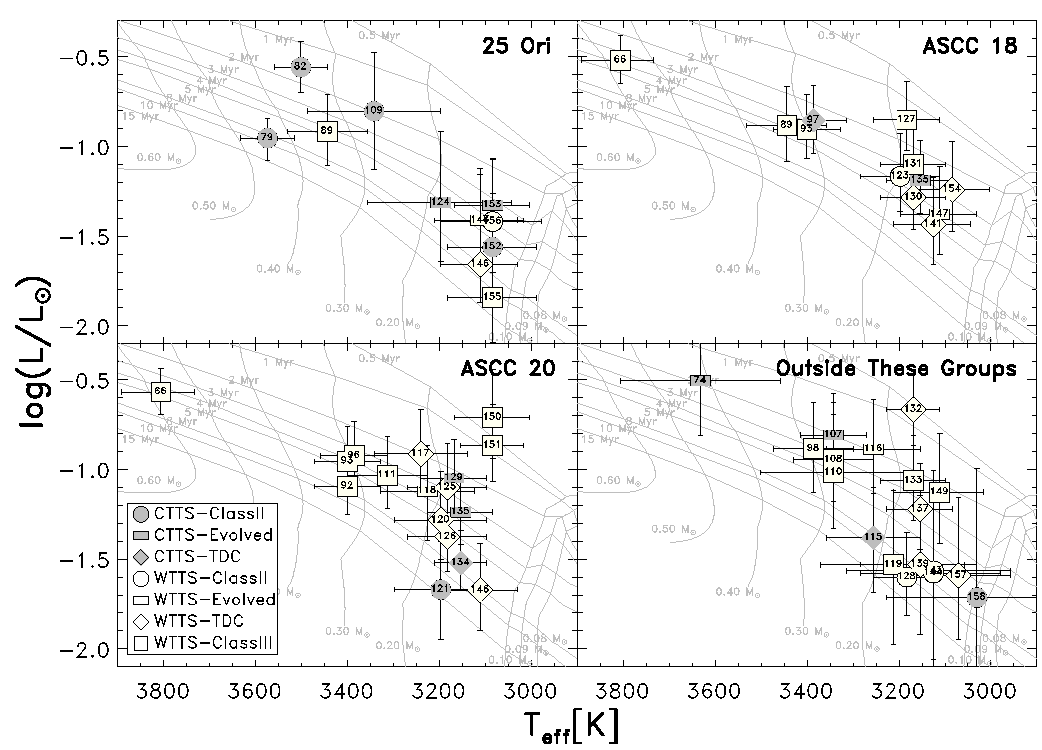
\includegraphics[width=1.\textwidth]{f6.pdf}
	\caption[H-R diagram of the confirmed members from the BOSS spectra]{H-R diagrams of the confirmed members inside the labeled stellar groups or outside them, according to \citet{Kharchenko2013}. The gray curves represent the PMS \citet{Baraffe2015} models. The members overlapping two of the stellar groups indicated in Figure \ref{fig_BOSS:sky} appear in both H-R diagrams.
	\label{fig_BOSS:H-R}}
\end{figure*}

\paragraph{Masses and Ages\\}

As shown in Figure \ref{fig_BOSS:H-R}, all members are scattered, within the uncertainties, throughout the 1-10 Myr isochrones and 0.1-0.6 M$_\odot$ evolutionary tracks, adopting the PMS models from \citet{Baraffe2015}.

To better estimate the masses and ages of the confirmed members, we interpolated their effective temperatures and bolometric luminosities into the \citet{Baraffe2015} models. When a confirmed member overlaps two stellar groups we adopted its mean bolometric luminosity. In Table \ref{tab_BOSS:parameters} we show the mass and age we obtained for each confirmed member. The resulting masses for the 53 confirmed members are in a range from 0.10 M$_\odot$ to 0.58 M$_\odot$, with $64\%$ of the members having masses lower than 0.20 M$_\odot$. This implies that in this mass range we increased by a $\approx50\%$ the number of confirmed LMSs in the region covered by the BOSS plate, and by a $\approx$20\% the number of LMSs in the estimated area of 25 Ori \citep[1$^\circ$ radius; ][]{Briceno2005,Briceno2007}.

The ages we calculated for the confirmed members are roughly twice younger than those found with similar methods in previous studies for the stellar groups where they are located \citep{Kharchenko2005,Briceno2005,Briceno2007,Kharchenko2013,Downes2014}. This is due to the target selection bias in the 25 Ori BOSS spectra (see Section \ref{sec_BOSS:spectroscopy} and Figure \ref{fig_BOSS:CCD_bias}).

For all the confirmed members we estimated the uncertainties in the derived values of the main physical parameters (extinction, effective temperature, bolometric luminosity, mass, and age) by considering the following factors: the error propagation that applies to each step described in this section and the errors associated to the interpolations. In Table \ref{tab_BOSS:parameters} we show the resulting uncertainties for the extinction, effective temperature, bolometric luminosity, mass, and age values for the confirmed members. We also indicate to which stellar group they belong.

\subsubsubsection{T Tauri Star Classification}
\label{sec_BOSS:TTSclass}

The BOSS low-resolution spectra allowed us to measure the H$_\alpha$ equivalent width, which we used, together with the spectral types, to classify the confirmed members as either accreting young LMSs (classical T Tauri stars; CTTSs) or non-accreting young LMSs (weak T Tauri stars; WTTSs). To define the limit between both types of T Tauri stars (TTSs), we adopted the empirical saturation criterion by \citet{BarradoYNavascues-Martin2003}, in which stars with H$_\alpha$ emission above this limit are classified as CTTSs, and otherwise as WTTSs. In Figure \ref{fig_BOSS:WHavsSpT} we show the TTS classification scheme and in Table \ref{tab_BOSS:parameters} we show the resulting classification for the whole sample of confirmed members.

We confirmed a total of 15 CTTSs and 38 WTTSs among the 53 members in the BOSS sample. This corresponds to a very high fraction of CTTSs to WTTSs compared to the values of 5.6\% and 3.8$\pm0.4$\% found by \citet{Briceno2007} and \citet{Downes2014}, respectively, which is due to the target selection bias toward sources with IR excesses.

\begin{figure}
	\begin{minipage}{0.60\textwidth}
		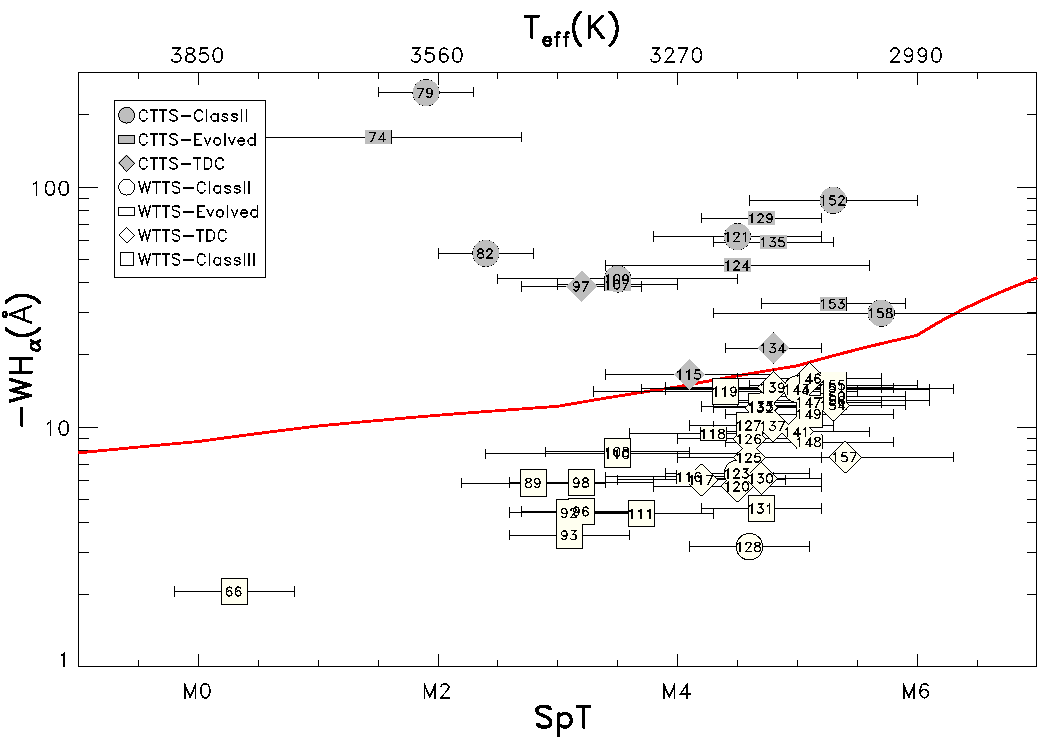
\includegraphics[width=1.0\textwidth]{f7.pdf}
	\end{minipage} \hfill
	\begin{minipage}{0.35\textwidth}
		\caption[TTS classification of the confirmed members from the BOSS spectra]{Relation between the H$_\alpha$ equivalent widths and spectral types for the confirmed members. The red solid curve indicates the saturation limit from \citet{BarradoYNavascues-Martin2003}, which allow us to separate WTTSs from CTTSs. The upper axis shows the effective temperature corresponding to the spectral types \citep{Luhman2003b}.}
		\label{fig_BOSS:WHavsSpT}
	\end{minipage}
\end{figure}

\subsubsubsection{Spectral Energy Distributions}
\label{sec_BOSS:SED}

The circumstellar disks of the YSOs were classified according to their IR excess emissions at $\lambda>2\ \mu$m. Objects having a flat or decreasing IR spectral energy distribution (SED) are considered Class II, while Class III objects have little or no near-IR excess \citep{Lada-Wilking1984,Lada1987}. An intermediate phase between the Class II and Class III objects contains the so-called ``transitional disk systems" that present a decreasing SED slope in the near-IR that rises again in the mid-IR. Finally, the ``evolved disk systems" show a monotonically decreasing IR SED \citep[e.g.,][]{Hernandez2007b}.

To classify the IR excesses of the confirmed members according to this scheme, we constructed their SEDs using the Virtual Observatory SED Analyzer (VOSA) tool \citep{Bayo2008} and the photometric catalogs described in Sections \ref{sec_BOSS:Optphot} and \ref{sec_BOSS:IRphot}, and listed in Table \ref{tab_BOSS:photometry}. We have a minimum of 10 and a maximum of 24 photometric bands for each confirmed member, covering a wavelength range from 0.36 $\mu$m to 22 $\mu$m.

The SEDs were dereddened using the visual extinction we estimated in Section \ref{sec_BOSS:extinction} and assuming the extinction law reported by \citet{Fitzpatrick1999} and subsequently improved by \citet{Indebetouw2005}. To determine the corresponding IR excesses we proceeded iteratively as follows: First, we fitted the SEDs to the PMS LMS models from \cite{Baraffe2015}, restricting the effective temperature range to the one obtained in Section \ref{sec_BOSS:HR}. During this iteration we only considered the photometric bands where the IR excesses are not expected to occur ($\lambda < 2\ \mu$m).

From the resulting fitted SEDs, VOSA automatically detects which bands present IR excesses by using an improved algorithm from that by \citet{Lada2006}, which measures the slope of the IR points in the log($\lambda F_\lambda$) vs log($\lambda$) space. Basically, when the slope becomes greater than -2.56, the IR excesses are determined.

Then, a second fit to the \cite{Baraffe2015} models was performed, this time excluding those photometric bands showing IR excesses. In this way, we avoided false IR excess detections during the first iteration and maximized the number of photometric bands used for fitting the photospheres. The number of photometric bands used during the second iteration ran from 10 to 23 (except for the members 74 and 109 with 7 and 8 fitted bands, respectively). In Figure \ref{fig_BOSS:SEDs} we show the resulting SEDs for a selection of the confirmed members. The bolometric luminosities for the confirmed members corresponding to the total flux of the best \citet{Baraffe2015} model fit are in agreement, within the uncertainties, with those obtained using the $I$ band, as explained in Section \ref{sec_BOSS:HR}.

\begin{figure*}[ht!]
	\centering
	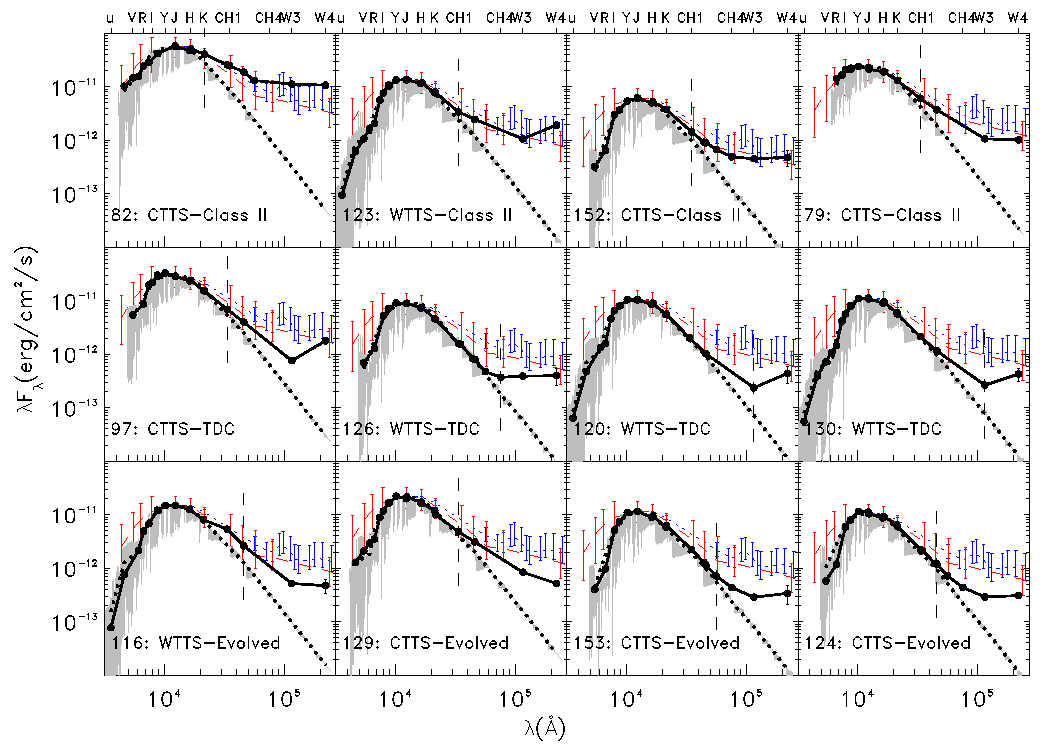
\includegraphics[width=1.0\textwidth]{f8.pdf}
	\caption[SEDs of the confirmed members from the BOSS spectra]{Dereddened SEDs for a sample of the confirmed members (black points and black solid curves). The gray spectra correspond to the best PMS LMS model from \citet{Baraffe2015} fitted to the dereddened data bluer than the point were the IR excesses start (vertical black dashed line). The black dotted curves show the fitted \citet{Baraffe2015} model spectra in a lower resolution. The red dashed curves and the blue dotted ones indicate, respectively, the median SEDs of Class II disks of the $\sigma$ Orionis cluster \citep{Hernandez2007a} and the Taurus star-forming region \citep{Furlan2006}, normalized to the dereddened $J$-band flux of each member. The vertical red and blue solid lines represent the upper and lower quartiles for these median SEDs. Each SED has a label with the member ID and its TTS and disk classifications, as explained in Sections \ref{sec_BOSS:TTSclass} and \ref{sec_BOSS:SED}, respectively. The photometric errors are included but most of them are smaller than the corresponding symbols. All the SEDs of the confirmed members are available in the electronic version of the \citealt{Suarez2017} publication.}
	\label{fig_BOSS:SEDs}
\end{figure*}

We classified the members as Class II if their IR SEDs resemble the median SEDs of Class II disks of the $\sigma$ Orionis cluster \citep{Hernandez2007a} and the Taurus star-forming region \citep{Furlan2006}. The members showing lower IR excesses were considered evolved systems, while the members having IR SEDs consistent with the photospheric \citet{Baraffe2015} model fit were classified as Class III. The members showing a near-IR SED consistent with evolved systems or Class III objects, but having an unexpected strong excess at 22 $\mu$m were considered as transitional disk candidates (TDC).

For the 14 members having available photometry in the [3.6] and [8.0] bands from IRAC, the slope in the [3.6]-[8.0] color ($\alpha$, in the log[$\lambda F_\lambda$] vs log[$\lambda$] space) was analyzed to improve the disk classification as follows \citep{Lada2006}: Class II objects have slopes of $-1.8<\alpha<0$; evolved or ``anemic" disk systems \citep{Hernandez2007a} have $-2.56\le\alpha<-1.8$ slopes; Class III objects have $\alpha<-2.56$. In Figure \ref{fig_BOSS:irac} we show the locations of the members in the IRAC color-color diagrams. All the CTTSs fall inside the CTTS locus defined by \citet{Hartmann2005}, but four objects classified as WTTSs also fall inside this region (two having evolved disks, one is a TDC and the other one is bearing a Class II disk). All the members located in the IR excess region defined by \citet{Luhman2005} have Class II disks and only one of them has an evolved disk. The rest of the evolved systems and TDCs are located in the region between the Class II and Class III objects, as expected from the \citet{Hernandez2007b} sample. 

\begin{figure*}[ht!]
	\centering
	\includegraphics[width=1.0\textwidth]{f9.pdf}
	\caption[IRAC color-color diagrams of the confirmed members from the BOSS spectra]{IRAC color-color diagrams for the confirmed members from this work (top panels) and including those from \citet{Hernandez2007b} (bottom panels). The small black filled circles, diamonds, horizontal bars and square represent YSOs with Class II, transitional, evolved or Class III disks from \citet{Hernandez2007b}. The dashed lines delimit the region where M type objects with disk are expected, from the study by \citet{Luhman2005}, and the dotted lines show the CTTS locus from \citet{Hartmann2005}.}
	\label{fig_BOSS:irac}
\end{figure*}

Of the 53 confirmed members we classified: $a)$ 11 Class II objects, with SEDs consistent with the $\sigma$ Orionis cluster and Taurus star-forming region median SEDs; $b)$ 10 evolved disks, showing decreasing IR excesses but smaller than the aforementioned medians; $c)$ 15 TDCs, having a sudden increase in their IR excesses at $22\ \mu$m; $d)$ 17 Class III, with no detectable IR excesses. In Table \ref{tab_BOSS:parameters} we list the final disk type classification for the LMS members. For the sources showing IR excesses, those start at the WISE 3.4 $\mu$m band (for $\approx 42$\% of them) or longer wavelengths. Only for one member (member 82), the IR excess starts in the $K$ band.

Considering both TTS and disk classifications for the 53 confirmed members: 17 out of the 38 WTTSs have disks of Class III, 12 are TDCs, 4 are evolved systems and 5 have Class II disks. All the 15 CTTSs show IR excesses, with 6 having Class II disks, 6 evolved systems and 3 TDCs.

\subsubsection{Peculiar Objects}
\label{sec_BOSS:singular}

\subsubsubsection{Variable Members}

Variability is an important effect than can be present in the member sample. It could modify their locations in the color-magnitude diagrams and affect the determination of physical parameters such as extinction, bolometric luminosity, mass, and age. We expect that the variability in the $I$ band should not have important effects in our confirmed member sample because we are using the CDSO photometric catalog, which lists mean magnitudes of multi-epoch observations with temporal spacing of about 4 yr. However, we are also working with multi-epoch VISTA photometry, which has temporal spacing of only 14 nights, where variability can be present. About $34\%$ of the confirmed members have $>99\%$ probability of being variable stars according to the CVSO catalog.

In the $I$ vs $I-J$ color-magnitude diagram, members 110, 116, 125, and 131 fall outside the region defined by the YSO candidates. None of these members is listed as a high-probability variable stars in the CVSO catalog. However, they show the greatest $J_\textrm{\tiny {VISTA}}-J_\textrm{\tiny {2MASS}}$ residuals (together with the high-probability variable stars 66, 74, and 118), with values of: 0.714, 0.357, 0.163, and 0.415 mag for members 110, 116, 125, and 131, respectively, which are, within the uncertainties, significantly larger than those for the rest of the members. These $J$-band differences explain well the deviated positions only for members 110 and 131. Members 110, 116, and 125 have close sources in the SDSS or 2MASS images, which may be contaminating their photometries, causing their deviations in the $I$ vs $I-J$ diagram.

\subsubsubsection{High-extinction Members}
\label{sec_BOSS:high_extinction}

Considering that the mean extinction toward 25 Ori is $\bar{A}_V\approx$0.28 mag \citep{Kharchenko2005, Briceno2005, Briceno2007, Downes2014}, members 74 and 109 present significantly higher extinction values of $A_V=4.33^{+0.51}_{-0.98}$ and $A_V=3.53^{+0.94}_{-1.01.}$ mag, respectively. These members are not high-probability variable stars in the CVSO catalog, although they have the largest $I-J$ colors in the sample. Furthermore, members 74 and 109 were classified as CTTSs showing, respectively, an evolved disk system and a Class II disk. Additionally, the spectra of these two members show IR emissions more intense than those for the confirmed members with the same spectral types but with low extinction values. It may be that their high-extinction values are caused by dust in their disks, which are presented to us with an edge-on geometry. The positions of these members in the H-R diagram are, within the uncertainties, consistent with most of the members. 

\subsubsubsection{Highly Luminous Members}

The deviant position of few members (132, 150, and 151) from the rest of the sample in the H-R diagrams can be naturally explained by their effective temperature and bolometric luminosity uncertainties. Only the member 132 is a $>99\%$ probability variable star according to the CVSO catalog. Members 132 and 150 have a close companion in the SDSS or 2MASS images, which can be contaminating their photometries. The member 151 may be an isolated star without signals of variability, indicating that its position in the H-R diagram could be real.

\subsubsection{Discussion and Conclusions}
\label{sec_BOSS:summary}

We determined the memberships of LMSs in the SDSS-III/BOSS spectra in 25 Ori and Orion OB1a on the basis of the presence of H$_\alpha$ emission and either LiI$\lambda$6708 or weak NaI$\lambda\lambda$8183, 8195 absorptions. We confirm 53 LMS members of 25 Ori or Orion OB1a, of which only three have been confirmed before by \citet{Downes2014}. These members are located in regions associated with at least three different stellar groups belonging to Orion OB1a \citep[25 Ori, ASCC 18, and ASCC 20; ][]{Kharchenko2005,Kharchenko2013}. The new LMS sample represents an increase of $\approx$50\% in the number of M0-M6 spectral type spectroscopically confirmed members in the area of the 25 Ori BOSS plate and a $\approx$20\% increase in the number of LMSs known inside the 25 Ori's estimated area \citep[1$^\circ$ radius; ][]{Briceno2005,Briceno2007}.

We did not confirm any K-type member in the 25 Ori BOSS plate on the basis of the H$_\alpha$ emission and LiI$\lambda$6708 absorption criteria. Furthermore, we found that the stars earlier than K-type are likely field stars after checking their position in the $I$ vs $I-J$ color-magnitude diagram and looking for their X-ray emission, IR excesses or variability.

Parallaxes for high-probability members from the \citet{Kharchenko2005} list are available from the Gaia DR1 catalog. Using these parallaxes, we derived distances of 336$\pm$30, 349$\pm$44, and 330$\pm$39 pc for 25 Ori, ASCC 18, and ASCC 20, respectively. Within the uncertainties, these stellar groups are located at the same distance (338$\pm$66 pc), but our estimates are based on a small number of high-probability members (17, 7, and 15 for 25 Ori, ASCC 18, and ASCC 20, respectively). With the next Gaia release we will have parallaxes for many more high-probability members and even for confirmed sub-solar members. 

The mean extinction (excluding two outliers) we calculated toward the whole member sample is $\bar{A}_V$=0.14 mag. If we only consider the members inside the 25 Ori area, we obtained $\bar{A}_V$=0.21 mag, which is slightly lower than the one in previous studies \citep[0.27 mag, 0.28 mag, 0.29 mag, and 0.30 mag by ][]{Kharchenko2005, Briceno2005, Briceno2007, Downes2014}. This small difference may be caused by the fact that our confirmed members in Orion OB1a span towards the south-east of the 25 Orionis star, where the \citet{Schlegel1998} extinction is even lower than in the area closer to the 25 Orionis star, as show in Figure 1 from \citet{Downes2014}. Members 74 and 109 have extinctions of $A_V=4.33^{+0.51}_{-0.98}$ and $A_V=3.53^{+0.94}_{-1.01.}$ mag, respectively, which are much higher than the mean. A likely explanation could be that these members present edge-on disks, similar to the BD 4 member from \citet{Downes2015}.

We constructed H-R diagrams for the confirmed members, assuming the distances determined from Gaia parallaxes. According to the PMS models from \citet{Baraffe2015}, the mass range covered by the members is from 0.10 M$_\odot$ to 0.58 M$_\odot$. We do not find a clear separation over the isochrones for the members located in the different stellar groups. The ages we estimated for the confirmed members are younger by a factor of $\sim 2$ than those for the stellar groups in which they lie \citep{Kharchenko2005,Briceno2005,Briceno2007,Kharchenko2013,Downes2014}. This is due to a bias in the target selection for the 25 Ori BOSS plate toward members with IR excesses. This bias is clear in Figure \ref{fig_BOSS:CCD_bias}, where most of the BOSS targets have $K$-W3 colors redder than those expected from previously confirmed members. 

Following the empirical saturation criterion by \citet{BarradoYNavascues-Martin2003} for the TTSs classification of the confirmed members, we found 38 WTTSs and 15 CTTSs. This number of CTTSs is very high, considering that the fraction of CTTSs in 25 Ori has a mean value of 4.7\% \citep{Briceno2007,Downes2014}, which is due to the bias in the selection of targets for the 25 Ori BOSS plate.

%We classified the 53 confirmed members as either WTTSs or CTTSs, following the empirical saturation criterion by \citet{Barrado2003}. We found a CTTS to WTTS fraction of about 40\%, which is very high compared with previous estimates of 5.6\% and 3.8$\pm0.4$\% by \citet{Briceno2007} and \citet{Downes2014}, respectively. Again, this high fraction of CTTSs is due to the bias in the BOSS target selection.

We constructed the SEDs of the TTSs and fitted the photospheric \citet{Baraffe2015} models in order to detect the IR excesses and classify their disks. We found: 11 Class II disks, with SEDs consistent with the median SEDs of Class II disks of the $\sigma$ Orionis cluster \citep{Hernandez2007a} and the Taurus star-forming region \citep{Furlan2006}; 10 evolved disks, with falling IR SEDs showing excesses smaller than the medians SEDs; 15 TDCs, with falling near-IR SEDs with a sudden increase in the mid-IR; and 17 Class III disks, with SEDs with no detectable IR excesses, consistent with the photospheric \citet{Baraffe2015} models. For the members showing IR excesses, these start at wavelength longer that WISE 3.4 $\mu$m (only for the member 82 these start in the $K$ band), which assure that the masses we assigned to the TTSs, working with the $I$ and $J$ bands, are not affected by the IR excesses.

The 34\% of the confirmed members are $>99\%$ probability variable stars in the CVSO catalog. This effect, together with close sources to the members in the SDSS and 2MASS images, explained well most of the deviated members in the $I$ vs $I-J$ color-magnitude diagram and H-R diagrams. Only the position of the member 151 in the H-R diagrams, that appears younger that expected, seems to be real. Additional analysis are necessary to reveal the nature of this object.

\subsubsubsection{Chromospheric Activity}
Due to the bias in the target selection for the 25 Ori BOSS plate, many of the confirmed members exhibit very strong H$\alpha$ emission. This intense emission is due to strong chromospheric (magnetic) activity for the WTTSs and a combination of this phenomenon with ongoing accretion for the CTTSs. A number of recent studies have demonstrated that chromospheric activity in LMSs can alter their physical properties relative to the expectations of non-magnetic stellar models. In particular, strong activity appears to be able to inflate the stellar radius and to decrease the effective temperature \citep[e.g. ][]{Lopez-Morales2007,Morales2008}. Typical amounts of radius inflation and effective temperature suppression are $\sim$10\% and $\sim$5\%, respectively \citep{Lopez-Morales2007}.

For PMS LMSs, these effects can be quite important, causing the stars to appear to have lower masses and younger ages. For example, \citet{Stassun2012} developed empirical relations for the radius inflation and effective temperature suppression for a given amount of chromospheric H$\alpha$ luminosity. These relations predict that the effective temperature suppression and radius inflation roughly preserve the bolometric luminosity. In addition, \citet{Stassun2014b} showed that the effect of effective temperature suppression on ensembles of young LMSs and BDs is to skew the inferred initial mass function strongly toward lower masses.  

In the case of the LMSs studied here, the individual ages we have determined for the entire sample are slightly younger than the mean estimated age of 25 Ori from previous studies. The combined effects of the effective temperature suppression from chromospheric activity as well as the bias in the target selection towards sources harboring disks, could explain such result. If so, then some of these stars could have higher masses and to be slightly older. This would have the effect of narrowing the age spread found here for these Orion OB1a groups. A detailed characterization of the mean ages of these regions is, however, beyond the scope of this work as it would require of a more robust sample of members.

\subsubsection{Appendix: Field Stars}
\label{appendix_BOSS}

The 119 objects resulting as field stars lack H$_\alpha$ emission and/or LiI$\lambda$6708 absorption, and show strong NaI$\lambda\lambda$8183, 8195 doublet in absorption. In Table \ref{tab_BOSS:field_stars} we list these stars rejected as confirmed members as well as their spectral types together with their $I$ magnitudes and $I-J$ colors.

\begin{table} \scriptsize
\begin{center}
 \caption[Stars on the BOSS plate rejected as confirmed members of 25 Ori or Orion OB1a]{Stars on the BOSS plate rejected as confirmed members of 25 Ori or Orion OB1a.}
 \label{tab_BOSS:field_stars}
 \begin{threeparttable}
  	\setlength{\tabcolsep}{20pt}
	\begin{tabular}{ccccc}
	\toprule
	{\bf RA} & {\bf DEC} & {\bf SpT} & $I$ & $I-J$ \\
	\midrule
	80.842323 & 1.310326 & A4.8  $\pm$3.6   & 16.587 & .494  \\
	82.423676 & 1.507883 & A5.1  $\pm$3.9   & 15.071 & .562  \\
	81.696971 & 0.706731 & A5.2  $\pm$3.7   & 15.134 & .530  \\
	82.240343 & 1.305623 & A5.3  $\pm$4.5   & 15.242 & .568  \\
	80.048167 & 1.076809 & A6.4  $\pm$4.8   & 14.051 & .551  \\
	82.15245  & 0.754426 & A6.7  $\pm$4.2   & 14.655 & .565  \\
	82.527304 & 1.605351 & A8.2  $\pm$5.4   & 15.897 & .605  \\
	80.51536  & 0.695541 & F0$^a$$\pm$---   & 16.268 & .543  \\
	80.049821 & 1.307561 & F0$^a$$\pm$---   & 18.248 & .598  \\
	81.607394 & 1.125553 & F0.5  $\pm$4.5   & 16.802 & .499  \\
	79.928433 & 1.42041  & F1.8  $\pm$5.2   & 14.876 & ---   \\
	82.211707 & 1.089703 & F2.2  $\pm$4.9   & 15.305 & .508  \\
	82.112572 & 1.021283 & F2.3  $\pm$5.1   & 15.757 & .524  \\
	\bottomrule
	\end{tabular}
	\begin{tablenotes}[para,flushleft]
	  {\bf Note.} The SDSS spectral type classification has not assigned the spectral type uncertainties.\\
	  $^a$ Spectral type assigned by the SDSS classification. Our SPTCLASS classification failed for this star.\\
	  (The complete version of this table is available in the electronic version of the \citealt{Suarez2017} publication.)\\
	\end{tablenotes}
 \end{threeparttable}
\end{center}
\end{table}

\subsection{MMT/Hectospec}
\label{sec:Hectospec}

\subsubsection{Hectospec Spectra}
\label{sec_hectospec:spectra}
To observed 25 member candidates with expected masses around the peak of its system IMF ($\approx0.3\ M_\odot$), we used the Hectospec multifiber spectrograph on the 6.5m MMT telescope at the MMT Observatory \citep{Fabricant2005}. Hectospec is a 300 optical fiber-fed spectrograph with a FOV of $0.5^\circ$ radius\footnote{\url{https://www.cfa.harvard.edu/mmti/hectospec/hecto_software_manual.htm}}. We obtained one night of MMT observing time and to prepare the observation we used the \texttt{xfitfib}s software\footnote{\url{https://www.cfa.harvard.edu/mmti/hectospec/xfitfibs/}} to create the fiber assigment of the Hectospec plates. The final design we considered consists of five Hectospec fields covering 25 Ori. Our observations were performed on two half-nights in 2016, one in October 4 and the other one in November 23 (PI: J. S. Kim). Only three of the five proposed fields were observed due to weather conditions. We show in Table \ref{tab:MMT_log} the log of our Hectospec observations and in Figure \ref{fig:sky_MMT} the design of the plates.
%The spectrograph setup used the 270 groove mm$^{-1}$ rating, resulting in a spectral resolution of $R\sim1000-2000$ with a spectral coverage from 3700 to 9150 \AA. 
%, each 1.5'' on the sky,

In addition to this data, we have been granted with Hectospec observing time for this semester to observe the remaining fields shown in Figure \ref{fig:sky_MMT}.

\begin{table} \scriptsize
\begin{center}
 \caption[MMT/Hectospec observing log]{MMT/Hectospec observing log.}
 \label{tab:MMT_log}
 \begin{threeparttable}
  	\setlength{\tabcolsep}{11pt}
	\begin{tabular}{ccccccc}
	\toprule
	{\bf UT Date}         & {\bf Field} & {\bf RA}     & {\bf DEC}    & {\bf Airmass} & {\bf T$_{exp}$} & {\bf No. targets} \\
	(yyyy-mm-ddThh:mm:ss) &             & (hh:mm:ss)   & (hh:mm:ss)   &               & (s)             &                   \\
	\midrule
	2016-10-04T11:35:38   & Plate 1     & 05:25:33.600 & 01:21:30.000 & 1.163         & 3x780           & 166               \\
	2016-11-23T09:35:54   & Plate 2     & 05:23:32.400 & 02:08:00.000 & 1.188         & 2x600$^a$       & 109               \\
	2016-10-05T12:09:28   & Plate 3     & 05:26:46.330 & 02:12:10.000 & 1.151         & 3x900           & 125               \\
	\bottomrule
	\end{tabular}
	\begin{tablenotes}[para,flushleft]
	  $^a$ Less time than requested but the spectra have enough SNR for our analysis.\\
	\end{tablenotes}
 \end{threeparttable}
\end{center}
\end{table}

\begin{figure}%[ht!]
	\includegraphics[width=1.0\textwidth]{sky_MMT.pdf}
	\caption[Plate design for the Hectospec observations.]{Proposed Hectospec fields (red circles) to observed young stellar candidates (14.5$<V\leq$18.5, 0.21$\leq m/M_\odot <$0.90) mainly in 25 Ori. Due to weather conditions, only the three plates with the higher priority were observed (red solid circles). The black dots and the gray dots represent the observed candidates and the remaining candidates, respectively, in the indicated mass range. Open symbols represent spectroscopically confirmed members from previous studies. The dashed circle indicates the 1$^\circ$ radius area of 25 Ori. The star symbol shows the position of the 25 Ori star.}
	\label{fig:sky_MMT}
\end{figure}

\subsubsubsection{Target Selection}
\label{sec_Hectospec:targets}
The candidates for the Hectospec observations were obtained from the selection by \citet{Downes2014}, which was done using optical-NIR color-magnitude diagrams in a similar way to our selection done in Su\'arez et al. (2018, submitted). With the three Hectospec plates we obtained 400 low-resolution spectra of member candidates with $V$-band brightness between 14.5 and 18.5 mag, corresponding to the mass range from 0.21 to 0.90 $M_\odot$, using the BT-Settl 7 Myr isochrone. In Figure \ref{fig:sky_MMT} we show the spatial distribution of the observed candidates inside the three Hectospec fields, which roughly cover the estimated area of 25 Ori.

\subsubsubsection{Data Reduction}
\label{sec_Hectospec:targets}
The raw data were downloaded from the distribution area at CfA, which also includes the calibration files (biases, dome and twilight flats and comparision lamp exposures). To reduce the spectra we used the IDL-based HSRED pipeline\footnote{\url{http://www.mmto.org/node/536}} originally developed by Richard Cool (MMTO) to work with Hectospec spectra using, basically, IRAF tasks. The pipeline produces one-dimensional, wavelength calibrated, sky subtracted, red-leak removed, and velocity correlated spectra. The spectra have a coverage from 3700 to 9150 \AA\ with a spectral resolution of $R\sim1000-2000$. In Figure \ref{fig:membership_MMT} we show an example of a Hectospec spectrum.

\begin{figure}%[ht!]
	\includegraphics[width=1.0\textwidth]{memberships_Hectospec.pdf}
	\caption[Hectospec spectrum of a confirmed member of 25 Ori.]{Hectospec spectrum of a confirmed member of 25 Ori. \textbf {Upper panel:} member spectrum with the original resolution of 6.0 \AA\ (gray solid line) and with a convolved resolution of 16 \AA\ (black solid line). \textbf {Lower panel:} Enlargements of the H$_\alpha$ emission, LiI$\lambda$6708 absorption and weak NaI$\lambda\lambda$8183, 8195 doublet youth indicators used to assign the memberships of the LMSs. The rest of the symbols and curves are as in Figure \ref{fig_BOSS:membership}. For this member, the spectrum presents H$_\alpha$ emission, LiI$\lambda$6708 absorption and the NaI$\lambda\lambda$8183, 8195 doublet consistent with the young stellar template. Therefore, this star was confirmed as a young LMS.}
	\label{fig:membership_MMT}
\end{figure}

\subsubsection{Spectra Analysis}
\label{sec_Hectospec:analysis}

\subsubsubsection{Spectral Types}
\label{sec_Hectospec:SpT}
To determined the spectral types of the Hectospec targets we used the SPTCLASS code, similarly than for the BOSS spectra in Section \ref{sec_BOSS:SpT}. The resulting spectral types range between K6.5 and M5.5, with an additional M7.0-type spectrum. The typical spectral type uncertainties for these sources are of 0.5 subclasses.

\subsubsubsection{Membership Assignment}
\label{sec_Hectospec:membership}
To determined the membership of the Hectospec spectra we worked with the H$_\alpha$ emission, LiI$\lambda$6708 absorption and weak NaI$\lambda\lambda$8183, 8195 absorption youth indicators, described in \citet{Suarez2017} (see Sections \ref{sec_BOSS:M_stars} and \ref{sec_BOSS:K_stars}). The equivalent widths of each spectral feature was obtained fitting a gaussian function to the observed line profile using \texttt{IRAF} tasks. Additionally, we also measured the equivalent widths directly from the SPTCLASS code, which are, as expected, consistent with those using IRAF.

So far, we have analyzed the spectra from Plate 2, resulting in 68 confirmed members, 52 of them by the first time. All these new members lie inside the 1$^\circ$ radius area of 25 Ori. The confirmed members already in the literature are: 1 from \citet{Briceno2007}, 7 from \citet{Downes2014}, 1 from \citet{Suarez2017} and 7 from \citet{Briceno2018}.

\subsubsubsection{Physical Parameters}
\label{sec_Hectospec:parameters}
We estimated the $T_{eff}$ of the confirmed members by interpolating their spectral types in the empirical relations from \citet{Kenyon-Hartmann1995}, \citet{Luhman1999}, \citet{Briceno2002} and \citet{Luhman2003b}.

We obtained the $A_V$, $L_{bol}$, mass and age of the Hectospec confirmed members in a similar way than for the members from the APOGEE-2 spectra, as explained in Section \ref{sec_APOGEE-2:parameters}. The mean $A_V$ we obtained is $0.35\pm0.29$, which is consistent with Su\'arez et al. (2018, submitted and references there in) and with that from the APOGEE-2 members. The mass range covered by these members is between 0.25 and 0.77 $M_\odot$. In Figure \ref{fig_Hectospec:HR} we show the H-R diagram of these resulting members. The mean age we obtained is $6.3\pm4.0$ Myr, which is in agreement with previous studies \citep[][ and references there in]{Briceno2018} and with the members from the APOGEE-2 spectra.

\begin{figure}[ht!]
	\includegraphics[width=1.0\textwidth]{HR_Hectospec.pdf}
	\caption[H-R diagram of the so far confirmed members from the Hectospec spectra.]{H-R diagram of the confirmed members from the Hectospec spectra. The grey curves represent the PARSEC evolutionary tracks for 0.2, 0.3, 0.4, 0.5, 0.6, 0.7 and 0.72 $M_\odot$ and the PARSEC-COLIBRI isocrones for 0.5, 1.0, 2.0, 3.0, 5.0, 10. and 30 Myr. The open symbol indicates the only member without mass and age estimates because lies outside the model grid.}
	\label{fig_Hectospec:HR}
\end{figure}

%comparing their $G_{BP}$-$G_{RP}$ observed colors from Gaia DR2 \citep{GaiaCollaboration2018} with the intrinsic colors obtained by interpolating $T_{eff}$ into the PARSEC-COLIBRI 7 Myr isochrone and then transforming the color excess to $A_V$ using the coefficients $C_{G_{BP}}=1.039$ and $C_{G_{RP}}=0.601$. The final mean $A_V$ for the confirmed members is $0.35\pm0.29$, which is consistent with Su\'arez et al. (2018, in prep. and references there in).

%The $L_{bol}$ of the confirmed members were obtained combining the $G$-band photometry and distances from Gaia DR2 with the $A_V$ to obtained the absolute magnitudes which were converted to $L_{bol}$ working with the bolometric corrections from \citet{Kenyon-Hartmann1995}.

%Then, we constructed the H-R diagram to obtained the masses and ages by interpolating into the PARSEC-COLIBRI isochrones. The final mass range coverd by the confirmed members goes from 0.25 to 0.77 $M_\odot$.

This analysis of the Hectospec spectra was done in collaboration with the undergraduate student Sandy Gonz\'alez as summer project during the ``XXVII Verano del OAN-SPM'' under my supervision.

%The spectral type classification, membership assignment and physical parameter estimates of these spectra were done as a summer project for the undergraduate student Sandy Gonz\'alez during the ``XXVII Verano del OAN-SPM'' under my supervision.
%in collaboration with the undergraduate student Sandy Gonz\'alez during the ``XXVII Verano del OAN-SPM'' under my supervision.

From the remaining two Hectospec plates without analysis (Plate 1 and Plate 3), which include 291 spectra, we expect to have about 182 additional members of 25 Ori of which roughly 140 of them should be confirmed by the first time.

\subsection{GTC/OSIRIS}
\label{sec:OSIRIS}

\subsubsection{OSIRIS Spectra}
\label{sec_OSIRIS:spectra}
To obtain spectra of the faintest member candidates of 25 Ori, expected to be very LMSs and BDs, we have ongoing observations with the Optical System for Imaging and low Resolution Integrated Spectroscopy (\ac{OSIRIS}) instrument mounted on the 10.4m GTC at Observatorio Roque de los Muchachos. As spectrograph, OSIRIS allows the acquisition of single long-slit or multiple object spectra in a FOV of 7x7 min$^2$ covering a wavelength range from 3650 to 10000 \AA\ with a maximum spectral resolution of 5000 \citep{Cepa2000,Cepa2003}. We worked with OSIRIS in the single long-slit mode (due to the low-density of targets in 25 Ori) with the R500R grism and a slit width of 1''. The observations being part of this thesis project were performed in service mode during five observing seasons between December, 2014 and November, 2018 (PIs: G. Su\'arez and C. Rom\'an-Z\'u\~niga) as part of the guaranteed Mexican time with GTC. Additionally, we have OSIRIS spectra of targets in 25 Ori and its surroundings taken during 2012 and 2013, which are part of the study by \citet{Downes2015}. In Table \ref{tab:OSIRIS_log} we show the log of all these OSIRIS observations.

\begin{table} \tiny
\begin{center}
 \caption{GTC/OSIRIS observing log.}
 \label{tab:OSIRIS_log}
 \begin{threeparttable}
  	\setlength{\tabcolsep}{11pt}
	\begin{tabular}{lccccccl}
	\toprule
	{\bf Target} & {\bf RA}    & {\bf DEC}    & {\bf UT Date}        & {\bf Airmass} & {\bf T$_{exp}$} & {\bf Seeing} &  {\bf Observing conditions} \\
	             & (hh:mm:ss)  & (hh:mm:ss)   &(yyyy-mm-ddThh:mm:ss) &               & (s)             & (arcsec)     &  (atmosphere/moon)          \\
	\midrule
	\multicolumn{8}{c}{{\bf 2012A Runs}} \\
	%1  & 05:23:09.86 & 01:42:50.8 & ---                     & --- & 3600 & ---      & ---                 \\
	%2  & 05:23:24.07 & 01:47:27.4 & ---                     & --- & 3510 & ---      & ---                 \\
	3  & 05:23:24.97 & 01:25:24.7 & 2012-03-12T21:02:06.050 & 1.3  & 3510 & ---      & ---                 \\
	%4  & 05:23:34.65 & 01:50:47.4 & ---                     & --- & 3410 & ---      & ---                 \\
	%5  & 05:23:48.34 & 01:48:33.1 & ---                     & --- & 3510 & ---      & ---                 \\
	%6  & 05:24:58.47 & 01:44:00.1 & ---                     & --- & 3510 & ---      & ---                 \\
	%7  & 05:22:49.69 & 02:11:51.0 & ---                     & --- & 3600 & ---      & ---                 \\
	\multicolumn{8}{c}{{\bf 2012B Runs}} \\
	8  & 05:23:09.86 & 01:42:50.8 & 2012-10-08T03:28:22.655 & 1.3  & 3440 & 1.10     & Clear/Grey          \\
	9  & 05:23:24.07 & 01:47:27.4 & 2012-10-08T04:32:45.348 & 1.2  & 3440 & 1.10     & Clear/Grey          \\
	10 & 05:23:34.65 & 01:50:47.5 & 2012-12-09T03:15:59.351 & 1.3  & 3440 & $<$1.0   & Spectroscopic/Dark  \\
	11 & 05:23:48.34 & 01:48:33.1 & 2012-12-17T01:06:16.672 & 1.1  & 3340 & 1.0      & Photometric/Dark    \\
	12 & 05:24:58.48 & 01:44:00.1 & 2012-12-17T03:24:48.060 & 1.4  & 3340 & 1.0      & Photometric/Dark    \\
	13 & 05:22:49.69 & 02:11:51.0 & 2012-12-21T21:25:13.901 & 1.6  & 3440 & 0.8      & Spectroscopic/Grey  \\
	14 & 05:25:36.62 & 00:54:55.5 & 2012-12-22T03:38:46.893 & 1.6  & 4602 & $<$0.8   & Spectroscopic/Grey  \\
	\multicolumn{8}{c}{{\bf 2013B Runs}} \\
	15 & 05:29:30.01 & 00:47:27.4 & 2013-10-13T05:02:08.778 & 1.1  & 3340 & 0.7      & Clear/Dark          \\
	16 & 05:29:13.80 & 00:51:10.2 & 2013-10-13T05:02:08.778 & 1.1  & 3340 & ---      & ---                 \\
	17 & 05:27:38.30 & 01:14:07.3 & 2013-10-14T05:01:06.925 & 1.1  & 3140 & $<$0.9   & Photometric/Bright  \\
	18 & 05:27:49.65 & 01:12:18.9 & 2013-10-14T05:01:06.925 & 1.1  & 3140 & ---      & ---                 \\
	19 & 05:27:24.15 & 01:38:01.8 & 2013-11-06T05:05:57.362 & 1.2  & 3240 & 0.7      & Spectroscopic/Dark  \\
	20 & 05:30:42.08 & 01:51:34.1 & 2013-11-05T04:39:54.909 & 1.2  & 3240 & 0.7      & Spectroscopy/Dark   \\
	21 & 05:30:35.45 & 01:46:30.0 & 2013-11-05T04:39:54.909 & 1.2  & 3240 & ---      & ---                 \\
	22 & 05:27:47.62 & 00:56:38.7 & 2013-11-06T01:50:38.996 & 1.3  & 3140 & 0.8      & Spectroscopic/Dark  \\
	23 & 05:27:38.19 & 00:57:41.7 & 2013-11-06T01:50:38.996 & 1.3  & 3140 & ---      & ---                 \\
	24 & 05:26:41.69 & 00:38:14.9 & 2013-11-06T04:15:15.002 & 1.1  & 3140 & 0.9      & Spectroscopic/Dark  \\
	25 & 05:26:35.63 & 00:36:01.7 & 2013-11-06T04:15:15.002 & 1.1  & 3140 & ---      & ---                 \\
	26 & 05:30:16.17 & 00:50:57.0 & 2013-11-07T02:23:33.637 & 1.2  & 3040 & 0.6      & Spectroscopic/Dark  \\
	27 & 05:26:11.95 & 00:49:15.5 & 2013-10-30T06:02:09.175 & 1.3  & 2940 & 0.8      & Clear/Dark          \\
	28 & 05:26:03.59 & 00:44:14.6 & 2013-10-30T06:02:09.175 & 1.3  & 2940 & ---      & ---                 \\
	\multicolumn{8}{c}{{\bf 2014B Runs}} \\
	29 & 05:23:34.66 & 01:50:47.9 & 2015-01-23T23:16:27.539 & 1.2  & 3906 & 0.7      & Photometric/Dark    \\
	30 & 05:23:48.37 & 01:48:32.5 & 2015-01-23T23:16:27.539 & 1.2  & 3906 & ---      & ---                 \\
	31 & 05:23:21.34 & 01:50:41.1 & 2014-12-26T01:27:10.108 & 1.2  & 4566 & 0.9      & Clear/Dark          \\
	32 & 05:23:24.07 & 01:47:27.7 & 2014-12-26T01:27:10.108 & 1.2  & 4566 & ---      & ---                 \\
	33 & 05:24:58.46 & 01:44:00.0 & 2015-01-21T23:17:01.712 & 1.2  & 3906 & 0.8      & Clear/Dark          \\
	34 & 05:25:08.74 & 01:46:32.1 & 2015-01-21T23:17:01.712 & 1.2  & 3906 & ---      & ---                 \\
	35 & 05:24:59.31 & 01:39:05.3 & 2014-12-29T02:10:27.281 & 1.4  & 3906 & 0.9      & Spectroscopic/Dark  \\
	36 & 05:24:41.44 & 01:35:51.7 & 2014-12-29T02:10:27.281 & 1.4  & 3906 & ---      & ---                 \\
	37 & 05:25:25.81 & 01:37:38.7 & 2014-12-29T00:50:12.894 & 1.2  & 3482 & 0.9      & Spectroscopic/Dark  \\
	38 & 05:25:20.91 & 01:37:14.3 & 2014-12-29T00:50:12.894 & 1.2  & 3482 & ---      & ---                 \\
	39 & 05:25:36.90 & 01:48:10.2 & 2014-12-26T03:04:16.605 & 1.6  & 4706 & 0.9      & Clear/Dark          \\
	40 & 05:25:14.67 & 01:48:39.4 & 2014-12-26T03:04:16.605 & 1.6  & 4706 & ---      & ---                 \\
	\multicolumn{8}{c}{{\bf 2015B Runs}} \\
	41 & 05:26:16.21 & 02:02:21.0 & 2015-12-04T01:44:13.496 & 1.1  & 4536 & 0.7      & Spectroscopic/Grey  \\
	42 & 05:26:12.99 & 02:06:26.0 & 2015-12-04T01:44:13.496 & 1.1  & 4536 & ---      & ---                 \\
	43 & 05:25:15.23 & 01:56:05.5 & 2015-12-04T03:27:58.254 & 1.3  & 3936 & 0.7      & Spectroscopic/Grey  \\
	44 & 05:25:28.85 & 01:59:49.0 & 2015-12-04T03:27:58.254 & 1.3  & 3936 & ---      & ---                 \\
	45 & 05:24:30.57 & 01:51:09.6 & 2015-12-11T01:09:42.745 & 1.1  & 3936 & 0.8      & Clear/Dark          \\
	46 & 05:24:28.27 & 01:53:27.5 & 2015-12-11T01:09:42.745 & 1.1  & 3936 & ---      & ---                 \\
	47 & 05:24:22.77 & 01:47:05.4 & 2015-12-11T01:51:49.910 & 1.1  & 4536 & 1.2      & Clear/Dark          \\
	48 & 05:24:07.87 & 01:48:01.7 & 2015-12-11T01:51:49.910 & 1.1  & 4536 & ---      & ---                 \\
	49 & 05:24:06.64 & 01:37:20.8 & 2015-12-12T23:46:30.718 & 1.2  & 3736 & 0.7      & Clear/Dark          \\
	50 & 05:24:04.32 & 01:35:18.4 & 2015-12-12T23:46:30.718 & 1.2  & 3736 & ---      & ---                 \\
	51 & 05:25:26.63 & 01:19:22.1 & 2015-12-13T00:54:46.712 & 1.1  & 3736 & 0.8      & Clear/Dark          \\
	52 & 05:25:24.66 & 01:21:26.5 & 2015-12-13T00:54:46.712 & 1.1  & 3736 & ---      & ---                 \\
	%\multicolumn{8}{c}{{\bf 2016A Runs}} \\
	%53 & 05:21:42.99 & 02:47:41.5 & ---                     & --- & 3990 & ---      & ---                 \\
	%54 & 05:21:40.15 & 01:50:24.0 & ---                     & --- & 3990 & ---      & ---                 \\
	%55 & 05:21:48.76 & 01:38:22.3 & ---                     & --- & 3990 & ---      & ---                 \\
	%56 & 05:25:08.81 & 02:05:05.5 & ---                     & --- & 3990 & ---      & ---                 \\
	%57 & 05:20:33.06 & 00:26:25.6 & ---                     & --- & 4890 & ---      & ---                 \\
	%58 & 05:23:34.26 & 01:05:51.1 & ---                     & --- & 3990 & ---      & ---                 \\
	\multicolumn{8}{c}{{\bf 2016B Runs}} \\
	59 & 05:21:42.99 & 02:47:41.5 & 2016-10-02T05:16:09.819 & 1.1  & 3990 & 1.0      & Clear/Dark          \\
	60 & 05:21:40.15 & 01:50:24.0 & 2016-10-11T05:13:19.736 & 1.1  & 3990 & 0.9      & Clear/Dark          \\
	61 & 05:21:48.76 & 01:38:22.3 & 2016-10-12T04:48:46.378 & 1.1  & 3990 & 0.7      & Clear/Dark          \\
	62 & 05:25:08.81 & 02:05:05.5 & 2016-11-24T03:38:30.210 & 1.2  & 3990 & 1.0      & Clear/Dark          \\
	63 & 05:23:34.26 & 01:05:51.1 & 2016-11-21T03:08:23.768 & 1.1  & 4350 & 1.2      & Spectroscopic/Dark  \\
	64 & 05:21:12.24 & 01:26:57.2 & 2016-12-06T00:20:53.845 & 1.2  & 4875 & 0.8      & Clear/Dark          \\
	\multicolumn{8}{c}{{\bf 2017B Runs}} \\
	65 & 05:22:18.67 & 02:05:53.2 & 2017-09-27T04:49:56.423 & 1.2  & 3375 & ---      & ---                 \\
	66 & 05:22:18.69 & 01:42:59.9 & 2017-09-28T04:24:37.194 & 1.2  & 3765 & ---      & ---                 \\
	67 & 05:22:23.84 & 01:42:25.2 & 2017-09-28T05:34:38.922 & 1.1  & 3675 & ---      & ---                 \\
	68 & 05:24:03.62 & 01:13:35.0 & 2017-09-29T04:15:19.030 & 1.3  & 3675 & ---      & ---                 \\
	69 & 05:26:01.78 & 01:39:15.5 & 2017-09-29T05:08:52.544 & 1.2  & 3675 & ---      & ---                 \\
	70 & 05:26:05.31 & 01:41:30.2 & 2017-11-24T01:47:50.305 & 1.1  & 3675 & ---      & ---                 \\
	71 & 05:26:43.16 & 01:31:23.6 & 2017-11-24T02:43:47.222 & 1.1  & 3375 & ---      & ---                 \\
	\multicolumn{8}{c}{{\bf 2018B Runs}} \\
	72 & 05:23:36.44 & 01:39:27.1 & 2018-10-03T04:46:47.796 & 1.2  & 3555 & 0.7      & Clear/Dark          \\
	73 & 05:26:01.80 & 01:39:14.8 & 2018-10-06T05:03:53.361 & 1.1  & 3555 & 1.1      & Spectroscopic/Dark  \\
	74 & 05:25:27.95 & 01:25:33.3 & 2018-10-15T05:08:56.785 & 1.1  & 3555 & 0.8      & Clear/Dark          \\
	75 & 05:26:45.60 & 01:39:00.7 & 2018-10-15T06:03:02.663 & 1.2  & 3555 & 0.9      & Clear/Dark          \\
	76 & 05:24:03.61 & 01:13:33.8 & 2018-10-16T05:50:14.268 & 1.2  & 3555 & 0.8      & Clear/Dark          \\
	77 & 05:26:43.18 & 01:31:23.1 & 2018-11-04T03:43:46.686 & 1.1  & 3555 & 0.7      & Clear/Dark          \\
	78 & 05:24:19.28 & 02:15:44.7 & 2018-10-31T05:21:56.865 & 1.2  & 3000 & 0.9      & Clear/Grey          \\
	\bottomrule
	\end{tabular}
	%\begin{tablenotes}[para,flushleft]
	%  $^a$ To be observed during semester 2018B.\\
	%\end{tablenotes}
 \end{threeparttable}
\end{center}
\end{table}

\subsubsubsection{Target Selection}
\label{sec_OSIRIS:targets}
For the OSIRIS observations during or before 2016, we selected from the \citet{Downes2014} candidate sample the faintest sources, which are expected to have spectral types between M6 and L1. This selection is based on the position on the sources in CMDs combining optical $I_c$-band photometry from the CDSO and NIR $J$, $H$ and $K$-band photometry from VISTA. During these observational seasons, we obtained OSIRIS spectra from 52 member candidates.

For the more recent OSIRIS observations, we selected from the candidate sample by Su\'arez et al. (2018, submitted) sources with the same expected spectral types (M6-L1). This sample is based in the position of the sources in the $I_c$ vs $I-J$ diagram with photometry from DECam and VISTA and includes candidates with expected masses down to 10 $M_{Jup}$. We have obtained OSIRIS spectra for 14 sources from this sample.% and we expect to have one extra spectrum during the rest of the year.

Considering all the observations with OSIRIS, we have spectra for 66 candidates to BDs, of which 55 lie inside the $1^\circ$ radius area of 25 Ori. In Figure \ref{fig_OSIRIS:sky} we show the spatial distribution of these targets. 

\begin{figure}[ht!]
	\includegraphics[width=1.0\textwidth]{sky_OSIRIS.pdf}
	\caption[Spatial distribution of the OSIRIS targets.]{Spatial distribution of the targets observed with OSIRIS (black solid points). The open circles indicate the spectra analyzed by \citet{Downes2015}. The dashed circle show the $1^\circ$ radius area of 25 Ori. The white star symbol indicates the position of the 25 Ori star. The background map is the same as in Figure \ref{fig_IMF:sky}.}
	\label{fig_OSIRIS:sky}
\end{figure}

\subsubsubsection{Data Reduction}
\label{sec_OSIRIS:reduction}
The raw data were downloading from the GTC FTP server together with calibration images (sky flats, dome flats, bias frames and comparison lamps) taken during the same night of observation. The spectra were reduced following the standard IRAF routines, which consist of bias and cosmic ray subtraction, flat-fielding, instrumental response correction, spectrum extraction, elimination of atmospheric spctral features and wavelength calibration. The resulting spectral coverage is between 5780 to 10000 \AA\ with a resolution of $R\approx1300$ at H$_\alpha$.

\subsubsection{Spectra Analysis}
\label{sec_OSIRIS:analysis}

\subsubsubsection{Membership Assignment}
\label{sec_OSIRIS:membership}
To determine the spectral types of the OSIRIS spectra we worked with the SPTCLASS semi-automatic code. So far, we have classified 58 spectra (88\%  of the full sample), obtaining spectral types between M6 and M9.5.

To assign the membership of the sources observed with OSIRIS, as mentioned by \citet{Downes2015}, we focused on the CaH, VO, KI and NaI features demostrated to be surface gravity sensitive in the optical spectra of BDs \citep{Martin1996}. The NaI$\lambda\lambda$8183, 8195 and the KI$\lambda\lambda7665, 7699$ doublets, and the CaH ($\lambda6750-\lambda$7050) molecular band are weaker in young dwarfs than in the field ones of the same spectral type, while the VO$^{\textrm{\scriptsize{I}}}$ ($\lambda7300-\lambda7500$) and the VO$^{\textrm{\scriptsize{II}}}$ ($\lambda7800-\lambda8000$) molecular bands are stronger in the young dwarfs \citep{McGovern2004}. We compared our OSIRIS spectra with the young stellar templates from \citet{Luhman2000}, \citet{Briceno2002}, \citet{Luhman2003b} and \citet{Luhman2004}, and the old field stellar templates from \citet{Kirkpatrick1999}. Additionally, we measured the equivalent width of the H$_\alpha$ line, which, when present in emission, supports the membership assignment.

After applying the above criteria to the 58 spectral type classified targets, we confirmed 42 BD members, including the 15 BDs by \citet{Downes2015}, of which 33 lie inside the area of 25 Ori. From the 27 new confirmed BDs, 26 of them lie inside the 1$^\circ$ radius area of 25 Ori. Additionally, we expect to have 6 more BD members with the recent OSIRIS spectra we obtained, falling all of them inside the spatial extent of 25 Ori. In Figure \ref{fig_OSIRIS:spectrum} we show the OSIRIS spectrum of one of these confirmed BDs in 25 Ori.

\begin{figure}%[ht!]
	\includegraphics[width=1.0\textwidth]{member_OSIRIS.pdf}
	\caption[OSIRIS spectrum of a BD confirmed to be member of 25 Ori.]{OSIRIS spectrum of a BD confirmed to be member of 25 Ori. The grey curve and the black curve represent the originally OSIRIS spectrum and the 16 \AA\ smoothed spectrum of the BD, respectively.}
	\label{fig_OSIRIS:spectrum}
\end{figure}

\subsubsubsection{Physical Parameters}
\label{sec_OSIRIS:parameters}
We obtained the $T_{eff}$ of the confirmed members by interpolating their spectral types in the relation by \citet{Pecaut2013}. For the estimation of $A_V$ we compared the observed $I_c-J$ colors from DECam and VISTA with the intrinsic colors obtained by interpolating $T_{eff}$ in the same mentioned relation to then convert the color excess to $A_V$ considering the coefficients by \citet{Cardelli1989}. To estimate $L_{bol}$, mass and age of the confirmed BDs we used the PHYPAR routine with the $I_c$-band magnitudes, assuming the 25 Ori distance obtained in this work ($356\pm47$ pc) and working with the BT-Sett isochrones. In Figure \ref{fig_OSIRIS:HR} we show the H-R diagram of the confirmed members using spectra from OSIRIS. The obtained masses range between 15 and 88 $M_{Jup}$. The resulting mean age from these members is $10\pm5$ Myr, which is slighly older than that obtained from the other confirmed members in this work and in the literature, but consistent within the uncertainties.

\begin{figure}%[ht!]
	\includegraphics[width=1.0\textwidth]{HR_OSIRIS.pdf}
	\caption[H-R diagram of the so far confirmed members with OSIRIS spectra.]{H-R diagram of the BDs and very LMSs confirmed in 25 Ori in this work (black squares) and by \citet[red circles; ][]{Downes2015}. The open symbols represent sources without mass and age estimates because lie outside the model grid. The grey curves show the BT-Settl evolutionary tracks of 0.011, 0.02, 0.05, 0.08 and 0.1 $M_\odot$ and isochrones of 0.5, 1, 2, 3, 5, 10 and 30 Myr. The black curve corresponds to the BT-Settl evolutionary track at the hydrogen burning limit mass (0.072 $M_\odot$).}
	\label{fig_OSIRIS:HR}
\end{figure}

\subsection{Summary of the Spectroscopic Survey}
\label{sec:spectra}
In this section we summarize and put together all the members we have confirmed using spectra from several world-wide facilities. We also discuss the completeness of the survey in terms of the estimated sources from the 25 Ori system IMF. 

The follow-up spectroscopy of the 25 Ori population was done as follow: $i)$ For sources with masses larger than $1.3\ M_\odot$, we obtained high-resolution spectra using MES at OAN-SPM, $ii)$ for candidates with masses in the range between 0.3 and 5.2 $M_\odot$, we obtained high-resolution spectra using APOGEE-2 from SDSS-IV, $iii)$ for candidates with masses between 0.09 and 0.7 $M_\odot$, we have low-resolution spectra taken with BOSS from SDSS-III, $iv)$ for LMS candidates in a similar mass range than the last mentioned, we have ongoing observations to acquire low-resolution spectra with Hectospec at the MMT, and $v)$ for the BD cadidates we have low-resolution spectra from OSIRIS at GTC. In Table \ref{tab:all_spectra} we summarize the number of spectra obtained with these spectrographs and in Figure \ref{fig:sky_all} we show the spatial distribution of all the observed targets.

\begin{table} \scriptsize
\begin{center}
 \caption{Details of the spectroscopic survey in 25 Ori.}
 \label{tab:all_spectra}
 \begin{threeparttable}
  	\setlength{\tabcolsep}{10pt}
	\begin{tabular}{@{\extracolsep{2pt}}lccccccc@{}}
	\toprule
	{\bf Spectrograph} & \multicolumn{2}{c}{{\bf Targets}} & \multicolumn{4}{c}{{\bf Confirmed Members}}            & {\bf $m$ range} \\
	\cline{2-3}
	\cline{4-7}
	                   & {\bf All} & {\bf 25 Ori$^a$}      & {\bf All} & {\bf 25 Ori$^a$} & {\bf By First Time$^b$} & {\bf Expected in 25 Ori$^c$} &                 \\
	                   &           &                       &           &                  &                         &                              & ($M_\odot$)     \\
	\midrule
	MES          & 77   & 50  & $>14^d$ & $>10^d$ & $>10^d$ & 36  & 1.3  - 11 \\
	APOGEE-2     & 1185 & 353 & 353     & 153     & 97      & 97  & 0.3  - 5.2  \\ 
	Hectospec    & 400  & 374 & $>68^e$ & $>68^e$ & $>52^e$ & 250 & 0.25 - 0.8  \\
	BOSS         & 172  & 68  & 53      & 26      & 23      & 23  & 0.09 - 0.7  \\
	OSIRIS       & 66   & 55  & $>42^f$ & $>33^f$ & $>26^f$ & 48  & 0.01 - 0.09  \\
	\bottomrule
	\end{tabular}
	\begin{tablenotes}[para,flushleft]
	  $^a$ Area of $1^\circ$ radius \citep{Briceno2005,Briceno2007} centered at $\alpha_{J2000}=81.2^\circ$ and $\delta_{J2000}=1.7^\circ$. \\
	  $^b$ Not in the spectroscopic studies by \citet{Briceno2005,Briceno2007,Downes2014,Downes2015,Suarez2017,Briceno2018}. For the members from BOSS spectra the comparison is not done with \citet{Suarez2017} because it is the publication of those members. \\
	  $^c$ Considering also the spectra without membership determination. \\
	  $^d$ From the analysis of 22 spectra (28\% of the sample). \\
	  $^e$ From the analysis of Plate 2, containing 27\% of all our Hectospec spectra. \\
	  $^f$ From the analysis of 58 spectra (88\% of the sample). \\
	\end{tablenotes}
 \end{threeparttable}
\end{center}
\end{table}

\begin{figure}[ht!]
	\includegraphics[width=1.0\textwidth]{sky_all_spectra.png}
	\caption[Spatial distribution of all the targets in our spectroscopic survey.]{Spatial distribution of all the targets observed with the spectrographs indicated in the label. The black circle shows the 1$^\circ$ radius area of 25 Ori. The background image is from the Digitized Sky Survey (DSS).}
	\label{fig:sky_all}
\end{figure}

Most of the targets were selected on the basis of their positions in CMDs combining optical and NIR photometry from different catalogs. In Figure \ref{fig:CMD_all} we show the $I_c$ vs $I_c-J$ CMD of the already observed targets in the spectroscopic survey. Most of the targets lying outside the PMS locus were observed by BOSS \citep{Alam2015} and are, in fact, field stars \citep{Suarez2017}.

\begin{figure}%[ht!]
	\includegraphics[width=1.0\textwidth]{CMD_targets.pdf}
	\caption[CMD of the targets with spectra.]{CMD of the targets observed using the facitilities indicated in the label. The black points show the member candidates selected in Section \ref{sec_IMF:locus} as the sources lying inside the PMS locus (black solid curves). The dashed and the dotted curves are the same as in Figure \ref{fig_IMF:CMD}.}
	\label{fig:CMD_all}
\end{figure}

The spectral types of the optical spectra were determined using the SPTCLASS semi-automatic code, which uses empirical relations between the spectral types and several spectral features sensitive to $T_{eff}$. For the NIR spectra from APOGEE-2, the $T_{eff}$ were obtained fitting synthetic spectra to the observed spectra \citep{Kounkel2018}.

The membership criteria we applied to the targets depend of their spectral types: $i)$ For the earlier stars we considered radial velocities and distance criteria (see Section \ref{sec_MES:membership}), $ii)$ for the early M and K-type stars we analyzed the H$_\alpha$ emission and the LiI$\lambda$6708 and NaI$\lambda\lambda$8183, 8195 absorptions (see Section \ref{sec_BOSS:M_stars}), and $iii)$ for the late M-type stars we focused on surface gravity sensitive features (see Section \ref{sec_OSIRIS:membership}). In Table \ref{tab:all_spectra} we indicate the number of confirmed members from the so far analyzed spectra and how many of them have been confirmed by the first time as well as the number of members we expect considering the remaining data.

To estimate the $A_V$ of the confirmed stellar members we worked with the $G_{BP}$ and $G_{GP}$ photometry from Gaia DR2 and for the confirmed BD members with $I_c$ and $J$ photometry from the DECam and VISTA catalogs. For the estimation of $L_{bol}$, mass and age of all these members, we used the PHYPAR code with the PARSEC-COLIBRI isochrones for members with masses larger than 0.2 $M_\odot$ and BT-Settl isochrones for lower masses. 

In Figure \ref{fig:flowchart} we summarize the general procedure followed to estimate the physical parameters of interest for most of the confirmed members and in Figure \ref{fig:HR_all} we show the H-R diagram of all the so far confirmed members in our spectroscopic survey, including the member candidates observed using MES as well as the spectroscopically confirmed members in previous studies by \citet{Briceno2005,Briceno2007,Downes2014,Downes2015,Briceno2018}. We emphasize that this H-R diagram includes sources in a spectral type range between M9.5 and B1, which corresponds to $T_{eff}$ between 2400 and 25000 K, considering the relation by \citet{Pecaut2013}. The total mass range covered by this sample is between 15 $M_{Jup}$ and 11 $M_\odot$. The mean age we obtained from the whole sample of sources in this H-R diagram is $6.5\pm3.5$ Myr, which is pretty consistent with previous studies \citep[6.1$\pm$2.4; ][ and references therein]{Briceno2018}.

\begin{figure}[ht!]
  \tikzstyle{decision} = [diamond, draw, fill=blue!50]
  %\tikzstyle{line} = [draw, -stealth, thick]
  \tikzstyle{line} = [draw, ->, line width=.2ex]
  \tikzstyle{trap} = [trapezium,trapezium left angle=70,trapezium right angle=-70,minimum height=3.9mm, draw, fill=green!20, text width=5.0em, text badly centered, node distance=2cm, inner sep=0pt]
  \tikzstyle{elli}=[draw, ellipse, fill=red!50,minimum height=5mm, text width=2em, text centered]
  \tikzstyle{block} = [draw, rectangle, fill=red!50, text width=3em, text centered, rounded corners, minimum height=10mm, node distance=5em]
  \tikzstyle{block0} = [draw, rectangle, fill=black!30, text width=4.0em, text centered, rounded corners, minimum height=10mm, node distance=5em]
  \tikzstyle{block1} = [draw, rectangle, fill=red!20, text width=6em, text centered, rounded corners, minimum height=10mm, node distance=5em]
  \tikzstyle{block1b} = [draw, rectangle, fill=red!50, text width=5em, text centered, rounded corners, minimum height=10mm, node distance=5em]
  \tikzstyle{block2} = [draw, rectangle, fill=red!20, text width=2em, text centered, rounded corners, minimum height=10mm, node distance=5em]
  \tikzstyle{block2b} = [draw, rectangle, fill=red!50, text width=2em, text centered, rounded corners, minimum height=10mm, node distance=5em]
  \begin{center}
  %\begin{tikzpicture}[remember picture, overlay, every node/.style={anchor=center}] \small
  \begin{tikzpicture}[remember picture, every node/.style={anchor=center}] \small
  	\node at (6,-0) [block2] (start) {SpT};
  	\node [block0, left of=start, xshift=-4.0em, yshift=0em] (Spectra) {\underline {\bf Spectra}};
  	\node [block2b, below of=start, xshift=-5em, yshift=-1em] (Teff) {$T_{eff}$};
  	\node [block2b, left of=Teff, xshift=-3em, yshift=0em] (RV) {RV};
  %	\node [block, right of=start, xshift=8em] (Gaia) {Gaia};
  	\node [block1, right of=start, xshift=13em] (Obser) {\scriptsize{$(G_{BP}-G_{RP})_{obs}$}};
  	\node [block1, right of=Teff, xshift=7em, yshift=0em] (Intrin) {\scriptsize{$(G_{BP}-G_{RP})_{int}$}};
  	\node [block1, right of=Intrin, xshift=6em, yshift=0em] (Excess) {\scriptsize{$E_{(G_{BP}-G_{RP})}$}};
  	\node [block2b, below of=Excess, xshift=0em, yshift=-1em] (Av) {$A_V$};
  	\node [block2, left of=Av, xshift=+0em, yshift=0em] (G) {$G$};
  	\node [block2, right of=Av, xshift=-0em, yshift=0em] (d) {$d$};
  	\node [block2, below of=Av, xshift=0em, yshift=0em] (MG) {$M_G$};
  	\node [block2, left of=MG, xshift=-1em, yshift=0em] (Mbol) {$M_{bol}$};
  	\node [block2b, left of=Mbol, xshift=-5em, yshift=0em] (Lbol) {$L_{bol}$};
  	\node [block1, below of=Teff, xshift=3em, yshift=-0em] (HR) {H-R Diagram};
  	\node [block1b, left of=Lbol, xshift=-9em, yshift=0em] (MassAge) {$mass,\ age$};
  	%arrows
  	\path [line] (start) -- (Teff);
  	\path [line] (Spectra) -- (start);
  	\path [line] (Spectra) -- (Teff);
  	\path [line] (Spectra) -- (RV);
  	\path [line] (Spectra) --+(-1.5,0) -- (RV);
  	\path [line] (Teff) -- (Intrin);
  	\path [line] (Intrin) -- (Excess);
  	\path [line] (Obser) -- (Excess);
  	\path [line] (Excess) -- (Av);
  	\path [line] (Av) -- (MG);
  	\path [line] (G) -- (MG);
  	\path [line] (d) -- (MG);
  	\path [line] (MG) -- (Mbol);
  	\path [line] (Mbol) -- (Lbol);
  	\path [line] (Teff) -- (HR);
  	\path [line] (Lbol) -- (HR);
  	\path [line] (HR) -- (MassAge);
  	%\path [line] (Lbol) -- (MassAge);
  	%\path [line] (Teff) -- (MassAge);
  	% arrows info
  	\node[opacity=1.0] at (4.4,0.0) {
  	        \includegraphics[width=1.5cm, height=0.4cm]{./Blue.png}
  	};
  	\node at (4.4,0.0) {\tiny{SPTCLASS}};
  	\node[opacity=1.0] at (2.5,-1.0) {
  	        \includegraphics[width=2.1cm, height=0.4cm]{./Blue.png}
  	};
  	\node at (2.5,-1.0) {\tiny{Synthetic spectra}};
  	\node[opacity=1.0] at (1.0,-0.4) {
  	        \includegraphics[width=0.8cm, height=0.4cm]{./Blue.png}
  	};
  	\node at (1.0,-0.4) {\tiny{IRAF}};
  	\node[opacity=1.0] at (12.8,1.0) {
  	        \includegraphics[width=1.3cm, height=0.4cm]{./Blue.png}
  	};
  	\node at (12.8,1.0) {\tiny{Gaia DR2}};
  	\node[opacity=1.0] at (5.1,-1.1) {
  	        \includegraphics[width=0.8cm, height=0.8cm]{./Blue.png}
  	};
  	\node at (5.1,-0.9) {\tiny{KH95}};
  	\node at (5.1,-1.3) {\tiny{PM13}};
  	\node[opacity=1.0] at (6.0,-2.3) {
  	        \includegraphics[width=2.3cm, height=0.4cm]{./Blue.png}
  	};
  	\node at (6.0,-2.3) {\tiny{PARSEC-COLIBRI}};
  	%\node at (6.0,-2.5) {\tiny{PM13}};
%  	\node[opacity=1.0] at (3,-1.1) {
%  	        \includegraphics[width=3.4cm, height=0.8cm]{./Blue.png}
%  	};
%  	\node at (3,-0.9) {\tiny{Kenyon \& Hartmann (1995)}};
%  	\node at (3,-1.3) {\tiny{Pecaut \& Mamajek (2013)}};
%  	\node[opacity=1.0] at (5.5,-2.3) {
%  	        \includegraphics[width=3.4cm, height=0.8cm]{./Blue.png}
%  	};
%  	\node at (5.5,-2.1) {\tiny{Kenyon \& Hartmann (1995)}};
%  	\node at (5.5,-2.5) {\tiny{Pecaut \& Mamajek (2013)}};
  	\node[opacity=1.0] at (11.0,-3.6) {
  	        \includegraphics[width=1.3cm, height=0.4cm]{./Blue.png}
  	};
  	\node at (11.0,-3.6) {\tiny{Gaia DR2}};
  	\node[opacity=1.0] at (12.9,-3.4) {
  		\includegraphics[width=4.3em, height=2.0em]{./Blue.png}
  	};
  		\node at (12.9,-3.2) {\tiny{$C_{G_{BP}=1.039}$}};
  		\node at (12.9,-3.6) {\tiny{$C_{G_{RP}=0.601}$}};
  	\node[opacity=1.0] at (14.8,-3.6) {
  	        \includegraphics[width=1.3cm, height=0.4cm]{./Blue.png}
  	};
  	\node at (14.8,-3.6) {\tiny{Gaia DR2}};
  	\node[opacity=1.0] at (13.0,-5.6) {
  		\includegraphics[width=9.4em, height=1.0em]{./Blue.png}
  	};
  		\node at (13.0,-5.6) {\tiny{$m_\lambda-M_\lambda=5\ log(d)-5+A_\lambda$}};
  	\node[opacity=1.0] at (11.8,-6.5) {
  		\includegraphics[width=1.8em, height=1.0em]{./Blue.png}
  	};
  		\node at (11.8,-6.5) {\tiny{BC$_\lambda$}};
  	\node[opacity=1.0] at (8.6,-5.7) {
  		\includegraphics[width=10.8em, height=1.0em]{./Blue.png}
  	};
  		\node at (8.6,-5.7) {\tiny{$M_{bol}-M_\odot=-2.5\ log(L_{bol}/L_\odot)$}};
  	\node[opacity=1.0] at (3.2,-5.4) {
  		\includegraphics[width=6.0em, height=2.0em]{./Blue.png}
  	};
  		\node at (3.2,-5.2) {\tiny{PARSEC-COLIBRI}};
  		\node at (3.2,-5.6) {\tiny{BT-Settl}};
  \end{tikzpicture}
  \end{center}
  	\caption[Scheme for the determination of physical parameters.]{Summary flowchart of the general procedure followed to estimate the physical parameters of interest of the confirmed members in our spectroscopic survey.}
  	\label{fig:flowchart}
\end{figure}

\begin{figure}%[ht!]
	\includegraphics[width=1.0\textwidth]{HR_25Ori.pdf}
	\caption[H-R diagram of all the so far confirmed members in this work and of the member candidates to high/intermediate mass stars.]{H-R diagram of the confirmed members using the spectra indicated in the label and of the member candidates observed using MES as well as of the previously confirmed members in the literature. The open symbols represent sources without mass and age estimates because lie outside the model grid. The grey curves represent the PARSEC evolutionary tracks of 0.3, 0.5, 0.7, 1, 1.5, 2, 3, 4, 5, 8 and 10 $M_\odot$ and the PARSEC-COLIBRI isochrones of 0.5, 1, 2, 3, 5, 10 and 30 Myr. The orange curves show the BT-Settl evolutionary tracks of 0.01, 0.02, 0.05, 0.08, 0.1 and 0.2 $M_\odot$ and isochrones of 0.5, 1, 2, 3, 5, 10 and 30 Myr. The black curve corresponds to the BT-Settl evolutionary track at the hydrogen burning limit mass (0.072 $M_\odot$). The upper axis shows the corresponding spectral types from \citet{Pecaut2013}.}
	\label{fig:HR_all}
\end{figure}

In Figure \ref{fig:completeness} we show the completeness of our spectroscopic survey in 25 Ori, also considering the members from the literature, according to the expected number of members from the tapered power law parameterization of its system IMF by Su\'arez et al. (2018, submitted). So far, the survey is $\sim75\%$ complete, with most of the remaining targest in the very LMS and BD regime. %To observe additional faint targets we plan to continue using OSIRIS and we have ongoing Hectospec observations in which we are going to include fainter sources than in the previous runs with this spectrograph. These results will allow us to construct, by the first time in a stellar association, the IMF with a statistically complete sample of spectroscopically confirmed members.

\begin{figure}%[ht!]
	\includegraphics[width=1.0\textwidth]{survey_completeness.pdf}
	\caption[Completeness of the follow-up spectroscopy in 25 Ori.]{Completeness of the follow-up spectroscopy in 25 Ori according to the expected members from its system IMF. The black curve shows the tapered power law parameterization by Su\'arez et al. (2018, submitted). The yellow dashed lines indicate the mass range covered by our different spectroscopic surveys, as indicated in the plot. The orange and blue filled histograms show the expected member coverage in several mass ranges by our follow-up spectroscopy and by the members in the literature, respectively, as indicated in the grey boxes. As reference, the black dashed lines show the edges of the 0.2 dex bins. The rest of lines and symbols are the same as in Figure \ref{fig_IMF:imf}.}
	\label{fig:completeness}
\end{figure}

%%%%%%%%%%%%%%%%%%%%%%%%%%%%%%%%%%%%%%%%%%%%%%%%%%
\section{Conclusions and Future Work}
\label{sec:conclusions}

\subsection{Conclusions}
In this work we characterized the stellar and substellar population of 25 Ori through photometric and spectroscopic analysis. Here we list the main results obtained from this analysis:\\

{\bf Photometry}
\begin{itemize}
	\item We selected, on the basis of color-magnitude and color-color diagrams combining optical and NIR photometry, a sample of 1687 member candidates in 25 Ori covering a mass range between 10 $M_{Jup}$ and 13 $M_\odot$ in a 1.1$^\circ$ radius area.
	\item With this sample of member candidates we constructed the 25 Ori system IMF from planetary-mass objects to intermediate/high mass stars, which is one of a few IMFs across the whole mass range of a stellar group.
	\item We fitted a triple power-law, a lognormal and a tapered power-law functions to the resultant system IMF to compare it with that in other stellar groups with a diversity of physical conditions. No significant differences were found, which suggests that the star formation process is largely insensitive to the enviromental conditions.
	\item We estimated that for each 7 stars in 25 Ori we roughly expect one BD. This value is similar for different radii between 0.4 and 1.1$^\circ$, which suggest that the substellar and stellar objects in 25 Ori have similar spatial distributions. Also, this BD/star ratio is consistent with that in other star-forming regions, which indicates that the formation of BDs and stars have a similar behaviour in different environments.
	\item We analyzed the behavior of the system IMF when considering member candidates inside different areas. The variation of the IMF parameters are contained within the uncertainties for radii between 0.4 and 1.1$^\circ$. This indicates that the substellar and stellar objects in 25 Ori do not have any preferential spatial distribution.
	\item Comparing the escape velocity of 25 Ori with its velocity dispersion, we confirmed that 25 Ori is a gravitationally unbound stellar group.
\end{itemize}

{\bf Spectroscopy}
\begin{itemize}
	\item We have an ongoing spectroscopic survey to observe each of the 25 Ori member candidates using several world-wide facilities: \par % We have the following data in 25 Ori: \par
		$i)$ 50 high-resolution spectra of intermediate/high mass stars using MES at the OAN-SPM. \par
		$ii)$ 353 high-resolution spectra of candidates with masses between 0.3 and 5.2 $M_\odot$ taken with APOGEE-2 from SDSS-IV. \par
		$iii)$ 374 low-resolution spectra of targets with masses from 0.25 to 0.8 $M_\odot$ using Hectospec at the MMT \par
		$iv)$ 68 low-resolution spectra of member candidates with masses ranging between 0.09 and 0.7 $M_\odot$ with BOSS from SDSS-III \par
		$v)$ 55 low-resolution spectra of very LMS and BD candidates using OSIRIS at GTC.
	\item Considering several youth spectral features for the LMSs and BDs and distance and radial velocity criteria for the intermediate/high mass stars, we have confirmed, so far, 290 members across the whole mass range of 25 Ori. 208 of these members are confirmed by the first time. Considering the remaining spectra without membership determination observed with MES, Hectospec and OSIRIS, we expect a total of 431 confirmed members in 25 Ori.
	\item We estimated the physical parameters (RV for the high-resolution spectra and $T_{eff}$, $A_V$, $L_{bol}$, mass and age for all the spectra). The mean RV, velocity dispersion, mean $A_V$ and mean age we obtained are consistent with previous studies and are based in a statistically more robust sample.
	\item From the sample of 53 confirmed members in 25 Ori and surroundings using spectra from BOSS, we analyzed their SEDs and classified their disks into evolutionary stages. We found that the IR excesses for sources harboring disks start at wavelengths larger than the $WISE\ 3.4\ \mu$m band.
	\item So far, our spectroscopic survey is $\sim75\%$ complete, considering the confirmed member and those expected from the spectra without membership determination as well as those confirmed in the literature. Most of the targets to be observed have expected masses around the hydrogen burning limit.
\end{itemize}

\subsection{Future Work}
As a continuation of the scientific analysis derived from this work, we list some of our plans for the near future:

\begin{itemize}
	\item The mass distribution we presented in this work is the system IMF, which is not corrected by multiple system. We plan to work with binarity properties obtained in the Orion Complex (Kounkel et al. 2019, in prep.) to study the effects of these systems in the determination of the single-star IMF.
	\item To complete the follow-up spectroscopy we are going to continue the observations with OSIRIS. Additionally, we have ongoing Hectospec observations, where we are going to include some of the faint targets without spectra. Also, we plan to submit observational proposals to other facilities such as FLAMES on the VLT, COSMOS on the Blanco 4-m telescope and/or Goodman on the SOAR 4.1-m telescope. 
	\item We are going to follow similar methodologies than described here to determine memberships and physical parameters of all the targets we have observed and those to be observed.
	\item With the statistically complete sample of spectroscopically confirmed members we plan to: \par
		Construct, by the first time in a stellar association, the spectroscopic-based IMF across the whole population. \par
		Analyze the kinematics, combining RVs from APOGEE-2 and MES with Gaia DR2, for the LMSs and intermediate/high mass stars to try to disentangle the presence of other associations overlapping 25 Ori, as suggested by \citet{Kounkel2018,Briceno2018}. \par
		Study the mass segregation effect in a relatively young group which could indicate the nature of this phenomenon; if it is a primordial property \citep{Bonnell-Davies1998,Bonnell2001} or due to dynamical evolution \citep{Kroupa2001a,Kroupa2001b} of clusters. This kind of study is also important to understand the BD formation mechanism because it is argued they are ejected objects during the earliest stages \citep{Reipurth-Clarke2001}. \par
		Analyze the age dispersion of the members to contribute to the understanding of this phenomenon to know until which degree it can be explained by the corresponding uncertainties or if it is a real effect \citep{Palla-Stahler1999,Palla-Stahler2000}. Also, we can look for any tendency of the ages with respect to the mass as a indicative than the formation of objects with certain masses occur first. \par
 %suggests if the formation of stars with different masses occurs at the same time or not. \par
		Study the frequency of the circumstellar disks in a wide mass range, from planetary-mass objects to intermediate/high mass stars (Downes et al. 2019, in prep.)
\end{itemize}

%%%%%%%%%%%%%%%%%%%%%%%%%%%%%%%%%%%%%%%%%%%%%%%%%%
%%%%%%%%%%%%%%%%% APPENDICES %%%%%%%%%%%%%%%%%%%%%
% Activate the appendix
% from now on sections are numerated with capital letters
\appendix

\section{Additional Contributions}
\label{sec:constributions}

\subsection{Collaborations}
\label{sec:collaborations}
Part of the data to carry out this thesis project was obtained working in collaboration in several studies. Additionally, valuable experience on the analysis of photometric and spectroscopic data was obtained participating in these collaborations. In this appendix I describe my constribution in each collaboration and how it is related to my thesis project.

\subsubsection{Ram\'irez-Preciado et al. 2018}
\label{sec:Ramirez-Preciado}
My main contribution in the \cite{Ramirez-Preciado2018} study was to estimate the physical parameters ($L_{bol}$, mass and age) for a sample of 571 candidates to belong to young nearby moving groups (YNMGs) to depurate the sample by removing post-MS star contaminants. This sample was obtained from chromospheric active stars in the Radial Velocity Experiment (RAVE) catalog \citep{Kunder2017}.

For this purpose, I used the PHYPAR routine with $T_{eff}$ and $A_V$ from RAVE, distances from the Gaia DR2 parallaxes and $J$-band magnitudes from 2MASS as well as $V$-band photometry from the AAVSO Photometric All Sky Survey (APASS) DR9 catalog \citep{Henden2016}, as a comparison. The resulting mass range of the sample is between 0.5 and 1.6 $M_\odot$. About 50\% of the candidates (290) have ages younger than 100 Myr, which is roughly consistent with the percentange of chromospheric active stars in RAVE that are high H$_\alpha$ emitters \citep{Zerjal2013}. This allowed us to remove about a half of the candidates, which have $M_V\ge4.5$ mag and lie in the post-MS in the H-R diagram. In Figure 8 from \citet{Ramirez-Preciado2018} we show the H-R diagram of the clear sample. This sample was used to identify YNMGs and/or to associate the candidates to previously identified YNMGs on the basis of kinematics criteria using the Cone Method \citep{Ramirez-Preciado2018}.

The experience I obtained working with this data allowed me to improve my own PHYPAR routine, which we are using for the estimation of the $L_{bol}$, mass and age of the resulting members of 25 Ori in our onging spectroscopic survey.

\subsubsection{Kounkel et al. 2018}
\label{sec:Kounkel}
As part of my collaboration with the APOGEE-2 Young Star Clusters working group, I contributed with the determination of the physical parameters ($A_V$, $L_{bol}$, mass and age) of the APOGEE-2 targets in the Orion Complex, which are distributed in several associations as $\lambda$ Ori, Orion A, Orion B, Orion OB1a and Orion OB1b. These results are part of the \citet{Kounkel2018} study about the 6D-structure of the Orion Star-forming Complex.

From the 8991 unique APOGEE-2 targets in the Orion complex, I selected about 4200 sources as highly probable member of the different Orion associations on the basis of their kinematics considering radial velocities from the APOGEE-2 spectra \citep{Kounkel2018} and proper motions from Gaia DR2, and their distances from Gaia DR2 parallaxes as well as their spatial distributions.

Working with the $T_{eff}$ estimated in \citet{Kounkel2018} and the $G_{BP}$ and $G_{RP}$ photometries from Gaia DR2, I estimated the visual extinctions of the highly probable members of the Orion Complex. Also, I estimated $A_V$ considering photometry from 2MASS. Additionally, I obtained the extinction values working with the dust maps from \citet{Schlegel1998}, \citet{Gontcharov2017}, \citet{Green2018} and from Herschel. After some comparisons between these extinctions, we decided to work with those from the Gaia DR2 data. I compared these $A_V$ from Gaia DR2 with those obtained by K. Stassun from spectral energy distribution fits and not significant differences were found.

I estimated the $L_{bol}$, mass and age of the highly probable members of the Orion Complex using the PHYPAR routine with the $T_{eff}$ from the APOGEE-2 spectra, the $A_V$ we obtained using Gaia DR2 data and the distances and $G$ magnitudes from Gaia DR2 as well as assuming the PARSEC-COLIBRI isochrones. Also, we obtained these parameters considering the $H$ magnitudes from 2MASS instead of the $G$-band photometry from Gaia DR2. At the end, when possible, we averaged the masses and ages obtained from both bands. The final mass range covered by the sample is between 0.13 and 5.2 $M_\odot$ and the ages for the full sample are shown in Figure 13 from \citet{Kounkel2018}. 

After the identification of spatially and/or kinematically distinct stellar groups in Orion, the ages obtained as described here allowed the investigation of the star-forming history in this complex \citep{Kounkel2018}. The identified populations have ages between 1 to 12 Myr.

The physical parameters of the highly propable members of 25 Ori obtained in this collaboration constitute part of the spectroscopic survey of my own thesis project.

\subsubsection{Cottle et al. 2017}
\label{sec:Cottle}
In the \citet{Cottle2018} collaboration, I participated in the selection of the Orion targets that were observed with the APOGEE-2 spectrograph. Particularly, I selected about 4500 photometric member candidates of Orion OB1a and OB1b on the basis of their positions in the $I$ vs $I-J$ and $I$ vs $I-K$ diagrams using photometry from the USNO and 2MASS catalogs (see Figures 15, 16 and 17 from \citealt{Cottle2018}). I considered as candidates the sources lying inside the defined PMS locus assuming the empirical isochrone traced by several spectroscopically confirmed members and highly probable members in the regions. Additionally, the target selection includes uniformly selected sources on the basis of IR excesses working with the 2MASS and WISE catalogs and variability from the PanSTARRS catalog as well as X-ray sources from the 3XMM-DR5 catalog. I worked in the design of the plates using a prioritization method to ensure the observation of the uniform selected sources, then of the X-ray sources and finally, to fill the remaining fibers, of the candidates from the CMDs.

For most of these targets, together with those in the $\lambda$ Ori, Orion A and Orion B associations, we obtained APOGEE-2 spectra, which are part of the \citet{Kounkel2018} study. 

The APOGEE-2 plates dedicated to 25 Ori (Ori OB1ab-E and OB1ab-F) were designed as part of this collabaration. These data are an important part of the 25 Ori ongoing follow-up spectroscopy in this thesis project.

\subsubsection{Richer et al. 2017}
%\subsection{\citealt{Richer2017}}
\label{sec:Richer}
I participated measuring the Full Width at Half Maximum (FWHM) of several spectral lines ([NII]$\lambda\lambda$6548,6583, HeII$\lambda$6560, H$_\alpha$ and CII$\lambda$6578) in high-resolution spectra of 76 planetary nebulae, most of them obtained from the San Pedro M\'artir Kinematic Catalogue of Planetary Nebulae \citep{Lopez2012}. These measurements were used in the \citet{Richer2017} study of the kinematics of the CII$\lambda$6578 permitted line with respect to the other mentioned lines to contribute to the understanding of the well-known abundance discrepancy problem.

For the measurements of the FWHMs of the lines of interest, I worked with \texttt{IRAF} tasks to fit gaussians to the observed line profiles. The experience I obtained from this study was applied to the analysis of the spectra in 25 Ori from the BOSS spectrograph \citep{Suarez2017}. Also, this ability is being used to analyze the spectra from the rest of the spectroscopic survey.

\subsubsection{Interdisciplinary Collaborations}
\label{sec:interdisciplinary_collaborations}
Due to my contribution in the selection of APOGEE-2 targets in the Orion Complex and in the analysis of these spectra as well as to my participation in the meeting of the APOGEE-2 Young Star Clusters working group, I am coauthor in the following papers: $i)$ 13th Data Release of SDSS \citep{SDSS-DR13}, $ii)$ SDSS-IV \citep{Blanton2017} and $iii)$ 14th Data Release of SDSS \citep{SDSS-DR14}.

%%%%%%%%%%%%%%%%%%%%%%%%%%%%%%%%%%%%%%%%%
\subsection{Proceedings}
\label{sec:proceedings}

\subsubsection{XV Latin American Regional IAU Meeting}
\label{sec:LARIM2016}
During the XV Latin American Regional IAU Meeting I presented my PhD thesis project and the status of the work, as described in \citet{Suarez2017b}. Also, I presented the analysis of low-resolution spectra in 25 Ori from the BOSS spectrograph, which are part of the \citet{Suarez2017} study.

\subsubsection{Francesco's Legacy: Star Formation in Space and Time}
\label{sec:SFST2017}
I presented in the \citet{Suarez2017c} contribution, during the Francesco's Legacy: Star Formation in Space and Time conference, the advances of the photometric determination of the system IMF of 25 Ori, stressing the importance and difficulties of removing the extragalactic contamination in deep photometric studies in this kind of stellar associations that present minimum extinction.

\subsubsection{Cool Stars 20}
\label{sec:CS20}
During the Cool Star 20 conference I presented in \citet{Suarez2018} the determination of the 25 Ori system IMF complete from 12 $M_{Jup}$ to 13.1 $M_\odot$. This presentation allowed to improve the discussion about the comparisons between this IMF and those in other clusters, as describe in the Su\'arez et al. (2018, submitted) study.

%%%%%%%%%%%%%%%%%%%%%%%%%%%%%%%%%%%%%%%%%
\section{PHYPAR Routine}
\label{sec_app:phypar}
{\scriptsize
\begin{Verbatim}[tabsize=4]
function phy_par, d, ed, T, eT, Av, eAv, Xmag, eXmag, BAND = band, MODEL = model, $
		 MIN_AGE = min_age, MAX_AGE = max_age, MIN_MASS = min_mass, MAX_MASS = max_mass, $
		 MAX_LBOL = max_Lbol

;+
; NAME:
;	phy_par()
; PURPOSE:
;	Estimate bolometric luminosity, mass and age of a set of targets
; EXPLANATION:
;	Using the distance, temperature, extinction and photometry of a set of 
;	sources, compute their bolometric luminosity, mass and age together 
;	with their uncertainties.
; CALLING SEQUENCE:
;	p	= phy_par(d, ed, T, eT, Av, eAv, Xmag, eXmag)
; INPUTS:
;	d		: distance in pc
;	ed		: distance uncertainties in pc
;	T		: temperature in K
;	eT		: temperature uncertainties in K
;	Av		: extinction in mag
;	eAv		: extinction uncertainties in mag
;	Xmag	: magnitude of the sources
;	eXmag	: magnitude uncertainties of the sources
; KEYWORD PARAMETERS:
;	band				: Photometric band of the input magnitude array. Options:
;		Vmag			: Vmag from Johnson
;		Rmag			: Rmag from Cousins
;		Imag			: Imag from Cousins
;		Gmag			: Gmag from Gaia
;		Jmag			: Jmag from 2MASS
;		Hmag			: Hmag from 2MASS
;		Kmag			: Kmag from 2MASS
;	model				: specify the models to be used. 
;		PARSEC-COLIBRI	: isochrones from Marigo et al. (2017)
;		BT-Settl 		: isochrones from Baraffe et al. (2015)
;	min_age				: youngest isochrone from the model (in yr)
;	max_age				: oldest isochrone from the model (to avoid the post-MS; in yr)
;	min_mass			: minimum mass to be used from the model (in Msun)
;	max_mass			: maximum mass to be used from the model (to avoid the 
;						  evolution of massive stars; in Msun)
;	OPTIONAL
;		max_bol			: maximum Lbol from the model to be considered to avoid post-MS 
;						  stages (when the model include them)
; OUTPUTS: an array containing Teff, Lbol, mass and age and their uncertainties
;
; EXAMPLE:
;	Obtain the Lbol, mass and age as well as their uncertainties for a set of targets, using the PARSEC-COLIBRI isochrones
;		p   = phy_par(d, ed, T, eT, Av, eAv, mag, emag, BAND = 'Vmag', MODEL = 'PARSEC-COLIBRI', min_age=age_mincut, $
;			          max_age=age_maxcut, min_mass=mass_mincut, max_mass=mass_maxcut)
;			T     = p[0,*]
;			eT    = p[1,*]
;			L     = p[2,*]
;			eL    = p[3,*]
;			mass  = p[4,*]
;			emass = p[5,*]
;			age   = p[6,*]
;			eage  = p[7,*]
;
; MODIFICATION HISTORY
;				by G. Suárez
;	11/09/18	Usage of the BT-Settl isochrones (Baraffe+2015)
; 				Usage of the Rc and Ic bands
;	05/07/18	Usage of the Gmag from Gaia
;	03/19/18	Avoid the code stops when there is not any generated Teff, Lbol 
;				inside the model grid. Mass and age errors are defined as 99.99.
;	03/17/18	Usage of the 2MASS bands.
;				Vmag not necessary in case of using 2MASS bands.
;	03/05/18	Output array has the same order as the input array.
; 	02/22/18	Uncertainty estimation improvement when doing interpolations.
; 	02/20/18	Improvement in the interpolation to obtain masses and ages.
; 	07/31/15	Uncertainty estimates.
; 	07/29/15	Development of the code by G. Suárez.

print,''
print,'%%%%%%%%%%%%%%%%%%%%%%%%%%%%%%%%%%%%%%%%%%%%%%%%%'
print,'%%%%%%%  Beginning of the phy_par code %%%%%%%%%%'
print,'%%%%%%%%%%%%%%%%%%%%%%%%%%%%%%%%%%%%%%%%%%%%%%%%%'
print,''

;#########################################################################
;#######################  FITTED PARAMETERS  #############################
;#########################################################################
																		;#
; Bolometric magnitude of the Sun.									  ;#
Mbol_sun	= 4.755  ; (Mamajek 2012)								   ;#
eMbol_sun	= 0.0004 ; error										   ;#
																	    ;#
; Extinction coefficients for the different filters.				    ;#
CI	= 0.751 ; A_R/A_V = 0.751 (Cardelli et al. 1989).				 ;#
CI	= 0.479 ; A_I/A_V = 0.479 (Cardelli et al. 1989).				 ;#
CJ	= 0.282 ; A_J/A_V = 0.282 (Cardelli et al. 1989).				 ;#
CH	= 0.190 ; A_H/A_V = 0.190 (Cardelli et al. 1989).				 ;#
CK	= 0.114 ; A_K/A_V = 0.114 (Cardelli et al. 1989).				 ;#
CG	= 0.9145; A_G/A_V = 0.9145 (J. Hernández private communication).  ;#
																	    ;#
;#########################################################################

; Extinction coefficients for the Xmag
if (band eq 'Vmag') then CXmag = 1.0
if (band eq 'Rmag') then CXmag = CR
if (band eq 'Imag') then CXmag = CI
if (band eq 'Jmag') then CXmag = CJ
if (band eq 'Hmag') then CXmag = CH
if (band eq 'Kmag') then CXmag = CK
if (band eq 'Gmag') then CXmag = CG

; Kenyon & Hartmann (1995) table.
filename_KH98	= 'files/Kenyon&Hartmann_1995_ApJ_101_117.cat'
readcol, filename_KH98, T_KH98, BCv_KH98, VR_KH98, VI_KH98, VJ_KH98, VH_KH98, VK_KH98, GJ_KH98, $
 format='x,x,x,f,f,x,x,f,x,f,x,f,f,f,x,x,x,x,f', comment='#'
	; V-Xmag color
	if (band eq 'Vmag') then VXmag_KH98	= replicate(0.0, N_elements(T_KH98))
	if (band eq 'Rmag') then VXmag_KH98	= VR_KH98
	if (band eq 'Imag') then VXmag_KH98	= VI_KH98
	if (band eq 'Jmag') then VXmag_KH98	= VJ_KH98
	if (band eq 'Hmag') then VXmag_KH98	= VH_KH98
	if (band eq 'Kmag') then VXmag_KH98	= VK_KH98
	if (band eq 'Gmag') then VXmag_KH98	= VJ_KH98 - GJ_KH98

	if (band eq 'Gmag') then begin
		ind	= where(GJ_KH98 ne 9999) ; remove the late SpT without G-J estimates
			T_KH98		= T_KH98[ind]
			BCv_KH98	= BCv_KH98[ind]
			VXmag_KH98	= VXmag_KH98[ind]
	endif

; MODELS
; PARSEC-COLIBRI (Marigo et al. 2017) isochrones with the UBVRIJHK photometry
if(model eq 'PARSEC-COLIBRI') then begin
	print, 'reading PARSEC-COLIBRI isochrones...'
	root_model	= 'files/Marigo_et_al._2017_ApJ_835_77/'
	file_model	= root_model+'isochrones.cat'
	readcol, file_model, age_model, mass_model, logL_model, logT_model, Mv_model, Mj_model, $
	 format='x,f,x,f,f,f,x,x,x,x,x,x,x,x,x,x,x,x,x,x,x,x,x,x,x,f,x,x,f,x,x', comment='#'
	
	L_model	= 10.^logL_model
	T_model	= 10.^logT_model
	
	; cut the isochrones in the specified mass range
	; keep ages between the specified range
	; remove some weird points with logL=-9.999
	ind	= where(mass_model gt min_mass and mass_model lt max_mass and age_model ge min_age and $
				age_model le max_age and L_model gt 10.^(-9.) and Mv_model-Mj_model lt 7.0)
	; also a luminosity cut to avoid post-MS stages
	if keyword_set(max_Lbol) then begin
		ind = where(mass_model gt min_mass and mass_model lt max_mass and age_model ge min_age and age_model $
					le max_age and L_model gt 10.^(-9.) and Mv_model-Mj_model lt 7.0 and L_model le max_Lbol)
	endif
		age_model	= age_model[ind]
		mass_model	= mass_model[ind]
		L_model		= L_model[ind]
		T_model		= T_model[ind]
endif
; BT-Settl (Baraffe et al. 2015) isochrones with the VRIJHK photometry
if(model eq 'BT-Settl') then begin
	print, 'reading BT-Settl isochrones...'
	root_model	= 'files/BHAC15/'
	file_model	= root_model+'isochrones.CIT2.cat'
	readcol, file_model, age_model, mass_model, T_model, logL_model, Mv_model, Mj_model, $
	 format='f,f,f,f,x,x,x,f,x,x,f,x,x,x,x,x', comment='#'
	
	age_model	= 1.e9*age_model ; yr
	L_model		= 10.^logL_model 

	; cut the isochrones in the specified mass range
	; keep ages between the specified range
	ind	= where(mass_model gt min_mass and mass_model lt max_mass and age_model ge min_age and age_model le max_age)
		age_model	= age_model[ind]
		mass_model	= mass_model[ind]
		L_model		= L_model[ind]
		T_model		= T_model[ind]
endif

;+++++++++++++++++++++++++++++++++++++
; Bolometric Luminosity
; deredden the observed magnitudes
Xmag_int	= Xmag - CXmag*Av

; convert intrinsic magnitudes to absolute magnitudes
MXmag	= Xmag_int - 5.0*alog10(d) + 5.0

; obtain the BCs interpolating Teff
BCv		= interpol(BCv_KH98, T_KH98, T)
VXmag	= interpol(VXmag_KH98, T_KH98, T) ; Vmag-Xmag intrinsic color
BCXmag	= BCv + VXmag ; BC of the X-band

; bolometric magnitude
Mbol	= MXmag + BCXmag

; bolometric luminosity
L	= 10.^((Mbol-Mbol_sun)/(-2.5)) ; (L/Lsun)

;+++++++++++++++++++++++++++++++++++++
; Prepare sources to obtain masses and luminosities
; keep only the sources inside the model grid to avoid extrapolations
PARSECCOLIBRIiso	= age_model(uniq(age_model)) ; isochrones
PARSECCOLIBRIiso	= PARSECCOLIBRIiso(sort(PARSECCOLIBRIiso)) ; sort the list of isochrones
N_iso				= N_elements(PARSECCOLIBRIiso) ; number of different isochrones

; index of the youngest and oldest isochrones
iso_youngest	= where(age_model eq PARSECCOLIBRIiso(0))
iso_oldest		= where(age_model eq PARSECCOLIBRIiso(N_iso-1))

; get the corresponding Lbol of the sources in the youngest and oldest isochrones
L_iso_y	= interpol(L_model(iso_youngest), T_model(iso_youngest), T)
L_iso_o	= interpol(L_model(iso_oldest), T_model(iso_oldest), T)

; keep sources older than the youngest isochrone and younger than the oldest isochrone
ind_in	= where(L le L_iso_y and L ge L_iso_o, nind_in, complement=ind_out, ncomplement=nind_out)

print,''
print,'There are '+strcompress(N_elements(T),/remove_all)+' sources in the input array'
print,'of which '+strcompress(nind_out,/remove_all)+' lie outside the model grid'
print,''
if(nind_in eq 0) then begin ; stop the code when there is none source inside the model grid
	print, 'All sources are outside the model grid'
	print,''
	stop
endif
print,''

;+++++++++++++++++++++++++++++++++++++
; MASS
; it is not necessary any sort of the model file
; the masses are the same (residual <0.035) using the isochrone file, track file or iso+track file.

; using the isochrones
; First triangulate the models' grids.
TRIANGULATE, alog10(T_model), alog10(L_model), tr_model
; determine mass interpolating T and L in the (logT, logL, m) grid of the model
mass_in	= GRIDDATA(alog10(T_model), alog10(L_model), mass_model, xout=alog10(T[ind_in]), $ 
			yout=alog10(L[ind_in]), TRIANGLES=tr_model, method='Linear') ; also NaturalNeighbor works well

;+++++++++++++++++++++++++++++++++++++
; AGE
; using the isochrones
; determine mass interpolating T and L in the (logT, logL, m) grid of the model
age_in	= GRIDDATA(alog10(T_model), alog10(L_model), age_model, xout=alog10(T[ind_in]), $ 
			yout=alog10(L[ind_in]), TRIANGLES=tr_model, method='Linear') ; also NaturalNeighbor works well

; mass and ages for the input array in the same order
mass	= fltarr(N_elements(T)) ; mass array to include the sources in and out of the model grid
age		= fltarr(N_elements(T)) ; age array to include the sources in and out of the model grid

mass[ind_in]	= mass_in ; estimated mass
age[ind_in]		= age_in ; estimated age
if(nind_out gt 0) then begin
	mass[ind_out]	= 99.99 ; for sources outside the model grid
	age[ind_out]	= 99.99 ; for sources outside the model grid
endif

;+++++++++++++++++++++++++++++++++++++
; UNCERTAINTIES
; deredden magnitude uncertainties
eAmag		= CXmag*eAv ; uncertaintiy of the Xmag extinction
eXmag_int	= sqrt(eXmag^2 + eAmag^2)

; absolute magnitude uncertainties
eMXmag	= sqrt(eXmag_int^2 + (5.*ed/(d*alog(10.)))^2)

; compute the BCv and V-Xmag uncertainties as the standard deviation of the 
; interpolated BCv and V-Xmag values from N-generated Teff for each source
eBCv		= fltarr(N_elements(BCv)) 
eVXmag 		= fltarr(N_elements(BCv))
N_ran		= 1e3 ; generated points
sigma_fac	= 1.0/3.0 ; relation between eTeff and std dev of the normal distribution
sigma		= (1.0/3.0)*eT ; std dev of the normal distribution to generate N-Teff
for i=0, N_elements(BCv)-1 do begin
	; BCv
	T_ran	= sigma(i)*randomn(seed, N_ran) + T(i) ; N-generated Teff with peak at the Teff of the source 
												   ; and std dev related with the Teff uncertainties
	BCv_ran	= interpol(BCv_KH98, T_KH98, T_ran) ; corresponding BCv for the N-generated Teff
	eBCv(i)	= stddev(BCv_ran) ; eBCv as the std dev of the interpolated BCv from the generated T
	; V-Xmag
	VXmag_ran	= interpol(VXmag_KH98, T_KH98, T_ran) ; corresponding V-Xmag for the N-generated Teff
	eVXmag(i)	= stddev(VXmag_ran) ; e(V-Xmag) as the std dev of the interpolated (V-Xmag) from the generated T
endfor

; BCXmag uncertainties
eBCXmag	= sqrt(eBCv^2 + eVXmag^2)

; bolometric uncertainties
eMbol	= sqrt(eMXmag^2 + eBCXmag^2)

; bolometric luminosity uncertainties
eL	= (alog(10.)/2.5)*L*sqrt(eMbol_sun^2 + eMbol^2)

; mass and age uncertainties with the same idea as for the BCv 
; uncertainties but with two gaussians (for eT and eL)
emass_in	= fltarr(N_elements(mass_in))
eage_in		= fltarr(N_elements(age_in))
sigma_T		= sigma_fac*eT[ind_in]
sigma_L		= sigma_fac*eL[ind_in]
for i=0, N_elements(ind_in)-1 do begin
	T_ran		= sigma_T(i)*randomn(seed, N_ran) + T(ind_in[i])
	L_ran		= sigma_L(i)*randomn(seed, N_ran) + L(ind_in[i])
	; keep only the (T, L) genereated points lying inside the youngest and oldest isochrone
	L_ran_iso_y	= interpol(L_model(iso_youngest), T_model(iso_youngest), T_ran)
	L_ran_iso_o	= interpol(L_model(iso_oldest), T_model(iso_oldest), T_ran)
	; estimate the masses and ages for the (T, L) points inside the model grid
	ind	= where(L_ran le L_ran_iso_y and L_ran ge L_ran_iso_o, nind)
		if(nind gt 0) then begin
			mass_ran	= GRIDDATA(alog10(T_model), alog10(L_model), mass_model, xout=alog10(T_ran(ind)), $
							yout=alog10(L_ran(ind)), TRIANGLES=tr_model, method='Linear')
			emass_in(i)	= stddev(mass_ran) ; mass uncertainties
			age_ran		= GRIDDATA(alog10(T_model), alog10(L_model), age_model, xout=alog10(T_ran(ind)), $
							yout=alog10(L_ran(ind)), TRIANGLES=tr_model, method='Linear')
			eage_in(i)	= stddev(age_ran) ; age uncertainties
		endif else begin
			emass_in(i)	= 99.99
			eage_in(i)	= 99.99
		endelse
endfor

; mass and ages uncertainties for the input array in the same order
emass	= fltarr(N_elements(T)) ; mass array to include the sources in and out of the model grid
eage	= fltarr(N_elements(T)) ; age array to include the sources in and out of the model grid

emass[ind_in]	= emass_in ; estimated mass
eage[ind_in]	= eage_in ; estimated age
if(nind_out gt 0) then begin
	emass[ind_out]	= 99.99
	eage[ind_out]	= 99.99
endif
param	= fltarr(8, N_elements(T))
	param[0,*]	= T
	param[1,*]	= eT
	param[2,*]	= L
	param[3,*]	= eL
	param[4,*]	= mass
	param[5,*]	= emass
	param[6,*]	= age
	param[7,*]	= eage

print,''
print,'%%%%%%%%%%%%%%%%%%%%%%%%%%%%%%%%%%%%%%%%%%%%%%%%%'
print,'%%%%%%%%%%  End of the phy_par code  %%%%%%%%%%%%'
print,'%%%%%%%%%%%%%%%%%%%%%%%%%%%%%%%%%%%%%%%%%%%%%%%%%'
print,''

return, param

end
\end{Verbatim}
}

%%%%%%%%%%%%%%%%%%%%%%%%%%%%%%%%%%%%%%%%%%%%%%%%%%
%%%%%%%%%%%%%%%%% REFERENCES %%%%%%%%%%%%%%%%%%%%%
\small
\setlength{\bibsep}{0pt plus 0.4ex}
\bibliography{mybib_Suarez} % if your bibtex file is called example.bib

%\thispagestyle{empty}
%
%\begin{center}
%\large {\bf \Large {Lista de Siglas y Acr\'onimos}}
%\end{center}
%
%FL : Funci\'on Luminosidad
%
%FMI : Funci\'on de Masa Inicial
%
%FMTP : Funci\'on de Masa al Tiempo Presente
%
%KTG93 : Kroupa, Tout \& Gilmore (1993)
%
%MS79 : Miller \& Scalo (1979)
%
%SP : Secuencia Principal
%
%TNE : Taza de Natalidad Estelar
%
%TPL : Tapered Power Law
%
%\newpage
%
%\section{Introducci\'on}
%\label{sec:introduccion}
%
%Cuando observamos el cielo nocturno, distinguimos una enorme cantidad de estrellas; algunas se encuentran aisladas, otras se encuentran atadas gravitacionalmente en sistemas m\'ultiples y otras parecen agruparse. Tambi\'en vemos estrellas con distintos brillos, relacionados con sus luminosidades y sus distancias, y con distintas temperaturas, relacionadas con sus masas y estado evolutivo. Las estrellas menos masivas tienen tiempos de vida m\'as prolongados en la Secuencia Principal (SP), mientras que las m\'as masivas evolucionan m\'as r\'apido.
%
%Las estrellas se forman en grupos a partir del colapso de gigantescas nubes moleculares. En estas poblaciones de estrellas se encuentran miembros con distintas masas, desde decenas de veces la masa de J\'upiter hasta decenas de veces la masa del Sol. Saber cu\'antas estrellas por intervalo de masa se forman en el nacimiento de una poblaci\'on estelar es uno de los objetivos de la astrof\'isica moderna, y como veremos, es uno de los ingredientes b\'asicos en el estudio de las poblaciones estelares en nuestra y otras galaxias.
%
%%Aunque se han desarrollado trabajos observacionales y te\'oricos muy importantes sobre cu\'al es la distribuci\'on que siguen las masas de las estrellas al nacer, todav\'ia persisten grandes interrogantes sobre cu\'ales son los procesos que regulan la formaci\'on de estrellas de distintas masas, c\'omo \'estas se combinan para resultar en esta distribuci\'on y, m\'as a\'un, y si son los mismos en todas las regiones de formaci\'on estelar.
%
%\subsection{Funci\'on de Masa Inicial}
%
%La distribuci\'on de las masas de las estrellas de una poblaci\'on estelar al momento de su formaci\'on se conoce como Funci\'on de Masa Inicial (FMI) y es, como ya veremos, una de las funciones de distribuci\'on m\'as importantes en astrof\'isica. Observacionalmente, la determinaci\'on de la FMI es complicada debido a que las masas estelares se miden indirectamente y, usualmente, no se puede observar el rango completo de masas estelares en una misma poblaci\'on estelar (e.g. Bastian \textit{et al.} 2010). Sin embargo, se han hecho una gran diversidad de trabajos sobre la FMI, algunos de los cuales revisaremos m\'as adelante.
%
%%La FMI de una poblaci\'on estelar es una propiedad que a\'un no se puede reproducir con exactitud con las teor\'ias de formaci\'on estelar. Una de las principales fuentes de incertidumbre son las condiciones iniciales, que por el momento s\'olo pueden ser determinadas a partir de las observaciones.
%
%
%\subsubsection{Determinaci\'on observacional de la FMI}
%\label{sec:determinacion_fmi}
%
%El primer paso para determinar observacionalmente la FMI de una poblaci\'on estelar es obtener una muestra completa de sus miembros a partir de conteos de estrellas.
%
%Al realizar conteos de estrellas en distintos tipos de poblaciones estelares (e.g. vecindad solar, c\'umulos estelares), la medici\'on directa que se obtiene es la distribuci\'on de brillos de sus estrellas, conocida como Funci\'on Luminosidad (FL, $\phi$), la cual se emplea para calcular la FMI. La FL se define como:
%
%\begin{equation}
%	dN=\phi(M_V)dM_V
%	\label{FL}
%\end{equation}
%donde \textit{dN} es el n\'umero de estrellas con magnitud visual absoluta entre $M_V$ y $M_V+dM_V$ en un volumen de un parsec c\'ubico. Para ejemplificar, la Figura \ref{fig:FL} muestra la FL en la banda visual para las estrellas de la vecindad solar.
%
%Ahora bien, para determinar cu\'antas estrellas se formaron en una poblaci\'on estelar por intervalo de masa (FMI), primero se necesita saber cu\'antas estrellas hay en la poblaci\'on por intervalo de masa en la actualidad, llamada Funci\'on de Masa al Tiempo Presente (FMTP). La FMTP se deriva de la FL a partir de una relaci\'on masa-$M_V$ que, usualmente, se basa en modelos de evoluci\'on estelar, y que es una manera simplificada de representar la relaci\'on entre las masas y las luminosidades de las estrellas (relaci\'on masa-luminosidad). En la Figura \ref{fig:m-Mv} se muestran ejemplos de relaciones masa-$M_V$ para las estrellas de la SP de la vecindad solar, obtenidas por Scalo (1986), Kroupa \textit{et al.} (1991) y Kroupa, Tout \& Gilmore (1993)(KTG93).
%
%\begin{figure}[H]
%    \begin{minipage}{0.49\linewidth}
%    \includegraphics[width=1\textwidth]{./pictures/Kroupa_1993_FL}
%    \caption{\emph{\footnotesize Distribuci\'on de brillo de las estrellas en la vecindad solar, obtenida por Wielen \textit{et al.} (1983) m\'as la extensi\'on hecha por KTG93 para M$_V\geq13$. La curva s\'olida representa la FL que KTG93 adoptaron. El eje vertical indica el n\'umero de estrellas dentro de una esfera de radio igual a 20 pc, lo que garantiza la completitud de las estrellas menos masivas.}}
%    \label{fig:FL}
%    \end{minipage}
%    \hfill
%    \begin{minipage}{0.49\linewidth}
%    \includegraphics[width=1\textwidth]{./pictures/Kroupa_1993_mass-Mv}
%    \caption{\emph{\footnotesize Relaciones masa-M$_\text{V}$ derivadas por KTG93 (curva s\'olida), por Kroupa \textit{et al.} (1991) (l\'inea a trazos) y por Scalo (1986) (l\'inea punteada). Los puntos s\'olidos indican los datos observacionales compilados por Popper (1980) y los c\'irculos vac\'ios por Liebert (1987).}}
%    \label{fig:m-Mv}
%    \end{minipage}
%  \end{figure}
%
%Luego, para pasar de la FMTP a la FMI necesitamos saber cu\'antas estrellas se produjeron en la poblaci\'on estelar a lo largo del tiempo, a lo que se conoce como Tasa de Natalidad Estelar (TNE). La forma de esta funci\'on depende de la poblaci\'on estelar que se considere. En la Figura \ref{fig:TNE} se muestran algunos tipos de TNEs que fueron analizadas por Miller \& Scalo (1979)(MS79).
%
%Para entender c\'omo la TNE corrige a la FMTP para obtener la FMI, consideremos estrellas que tienen un tiempo de vida en la SP menor que la edad de la Galaxia. En este caso, la FMTP se debe aumentar por alguna cantidad debido a las estrellas que ya salieron de la SP, dependiendo de la forma de la TNE. Para una TNE que decrece r\'apidamente con el tiempo (Figura \ref{fig:TNE}a-b), una gran cantidad de estas estrellas habr\'an salido de la SP, por lo que la correcci\'on de la FMTP para obtener la FMI, en este caso, ser\'a mayor. Por el contrario, si la TNE aumenta r\'apidamente con el tiempo (\ref{fig:TNE}d-f), ser\'an pocas las estrellas que hayan salido de la SP, por lo que la FMTP ser\'a ligeramente menor que la FMI y, la correcci\'on para pasar a la FMI, en este caso, ser\'a menor. Si ahora consideramos estrellas con tiempos de vida en la SP mayores que la edad de la Galaxia, la FMI y la FMTP son equivalentes. 
%
%\begin{figure}[H]
%  \centering
%    \includegraphics[width=.6\textwidth]{./pictures/TNE}
%    \caption{\emph{\footnotesize TNE respecto a la TNE promedio, b(t), como funci\'on de la fracci\'on del tiempo t con respecto a la vida de la Galaxia T$_0$. a) Ley de potencia con exponente 2, usada por Schmidt (1959); b) exponencial decreciente, es una de las formas m\'as usadas en la literatura (e.g. Tinsley 1974); c) constante, fue usada por Salpeter (1955); d) exponencial creciente; e) exponencial creciente asint\'oticamente; y f) polinomio. Las \'ultimas tres TNE's fueron estudiadas por MS79.}}
%    \label{fig:TNE}
%\end{figure}
%
%Una vez que se tiene una estimaci\'on de la FMI es importante determinar una forma funcional y los par\'ametros que mejor la representen para poder hacer comparaciones de su forma en distintas poblaciones estelares.
%
%\subsubsection{Parametrizaci\'on de la FMI}
%\label{sec:parametrizaciones}
%
%La FMI es un ingrediente importante para conocer las propiedades y la evoluci\'on de las poblaciones estelares. Adem\'as, la FMI es imprescindible para estudiar las propiedades integradas de poblaciones lejanas como para poder resolver sus miembros.
%
%A continuaci\'on se describen las parametrizacion m\'as usadas en la literatura para la FMI.\\
%
%{\bf Salpeter (1955)}\\
%
%El trabajo inicial sobre la FMI fue hecho por Salpeter (1955) con estrellas de la vecindad solar. Las hip\'otesis que formul\'o son que las estrellas salen de la SP despu\'es de consumir cerca del 10\% de su masa de H y que la TNE ha sido uniforme en la vecindad solar durante los \'ultimos 5 Ga\~nos\footnote {\emph{\footnotesize En lo sucesivo usaremos los prefijos del Sistema Internacional de Unidades para representar cantidades.}}. La Figura \ref{fig:salpeter} muestra la forma de la FMI ($\xi(m)$) que obtuvo Salpeter (1955), donde se puede observar que la relaci\'on logar\'itmica entre la masa y log$\xi(m)$ no tiene cambios marcados en su pendiente en el intervalo de log(\textit{m}) entre -0.4 y 1.0 M$_\odot$ (0.4$\lesssim m/M_\odot\lesssim10$). Adem\'as, esta relaci\'on presenta una ca\'ida intensa para masas mayores que 10 M$_\odot$, lo cual no es claro si es un efecto real o es el sesgo que impone que la muestra de la vecindad solar posee pocas estrellas con estas masas. En base a la forma constante de esta relaci\'on, Salpeter encontr\'o que la FMI se puede escribir como la siguiente ley de potencias: 
%
%\begin{equation}
%	\xi(m)=\frac{dN}{dm}=k_1m^{-\alpha}
%	\label{eq:Salpeter}
%\end{equation}
%
%donde $d$N es el n\'umero de estrellas en el intervalo de masas entre \textit{m} y \textit{m+dm}, \textit{k$_1$} es una constante de normalizaci\'on y $\alpha$ es el par\'ametro que caracteriza esta forma de la FMI. Alternativamente, esta ecuaci\'on se puede escribir como funci\'on del logaritmo de la masa, como se indica en la Ecuaci\'on \ref{eq:Salpeter_log}.
%
%\begin{equation}
%	\xi(\log(m))=\frac{dN}{d(\log(m))}=k_2m^{-\Gamma}, \hspace*{1cm} \textrm{donde} \hspace*{1cm} \Gamma=\alpha-1
%	\label{eq:Salpeter_log}
%\end{equation}
%
%Para las constantes de normalizaci\'on se emplearon nombres distintos para aclarar su diferencia. \textit{En lo sucesivo, usaremos a $\alpha$ como el par\'ametro que determina la pendiente del la ley de potencias.}
%
%Los valores de los par\'ametros que Salpeter (1955) report\'o  para la forma de la FMI de las estrellas de la vencidad solar son $\alpha$=2.35 y $k_1$=0.01 para el intervalo de masa 0.4$\lesssim m/M_\odot\lesssim10$.
%
%\begin{figure}[H]
%  \centering
%    \includegraphics[width=.5\textwidth]{./pictures/Salpeter_1955}
%    \caption{\emph{\footnotesize Logaritmo de $\xi(m)$ versus el logaritmo de la masa seg\'un el trabajo de Salpeter (1955). Esta curva pasa por todos los puntos de la muestra, excepto por los c\'irculos se\~nalados. El eje superior muestra la magnitud absoluta M$_V$ correspondiente al logaritmo de las masas de las estrellas.}}
%    \label{fig:salpeter}
%\end{figure}
%
%
%{\bf Miller \& Scalo (1979)}\\
%
%Considerando la forma de la FMI propuesta por Salpeter (1955), se espera que el n\'umero de objetos aumente cada vez m\'as conforme disminuye su masa. Sin embargo, MS79 trabajando con estrellas del disco en la vecindad solar y suponiendo que la FMI es independiente del tiempo y que es una funci\'on continua con la masa, buscaron una representaci\'on de la FMI que describiera la ca\'ida observada en el r\'egimen de baja masa, la cual no era predicha por la parametrizaci\'on de Salpeter (1955). MS79 analizaron las TNEs mostradas en la Figura \ref{fig:TNE}, encontrando que la forma constante es consistente con la mayor\'ia de los escenarios te\'oricos para la historia de la TNE. Considerando estas TNEs, MS79 encontraron que la FMI es bien aproximada por una distribuci\'on log-normal para masas en el intervalo $0.1\leq m/M_\odot\leq50$, como se indica en la Ecuaci\'on \ref{eq:MS79}.
%
%\begin{equation}
%	\xi(\log(m))=C_0\exp[-C_1\left(\log(m)-C_2\right)^2] 
%	\label{eq:MS79}
%\end{equation}
%
%donde 
%
%\hspace*{1.0cm}$C_0 = 66.20$, $C_1 = 1.15$ y $C_2 = -0.88$ considerando una TNE que aumenta con el tiempo.
%
%\hspace*{1.0cm}$C_0 = 106.0$, $C_1 = 1.09$ y $C_2 = -1.02$ considerando una TNE contante.
%
%\hspace*{1.0cm}$C_0 = 242.4$, $C_1 = 1.14$ y $C_2 = -0.93$ considerando una TNE que decrece con el tiempo.\\
%
%La FMI que MS79 determinaron para las estrellas de la vecindad solar est\'a en acuerdo con la FMI de los c\'umulos estelares en el rango de masa $1.0< m/M_\odot<10$, pero algunos c\'umulos tienen un d\'eficit de estrellas de baja masa. Para $m\geq$2.5 M$_\odot$, esta FMI log-normal  empata bien con la FMI para la asociaci\'on OB1 de Ori\'on (MS79).
%
%Existen ligeras diferencias entre la pendiente de Salpeter (1955) y la log-normal de MS79 debido, principalmente, a que MS79 mejoraron los tiempos de vida de las estrellas en la SP, y a que Salpeter (1955) consider\'o s\'olo estrellas del disco gal\'actico y no integr\'o en la direcci\'on perpendicular al plano.\\
%
%
%{\bf Scalo (1986)}\\
%
%Scalo (1986) trabaj\'o con poblaciones de estrellas de la vecindad solar, asociaciones estelares, c\'umulos estelares y galaxias, encontrando similitudes entre sus FMIs. Las principales conclusiones que obtuvo sobre las FMIs de estas poblaciones estelares son:
%
%\textit{i)} La FMI para las estrellas de la vecindad solar alcanza su pico en $m\approx 0.3 \text{ M}_\odot$ y disminuye para masas menores. El exponente de la ley de potencias para las estrellas masivas es $\alpha \sim 2.7$, aunque para $m> 10 \text{ M}_\odot$ es incierto.
%
%\textit{ii)} Para las estrellas del disco y del halo de la vecindad solar, la FMI es muy similar en el rango de masa $0.3\leq m/\text{M}_\odot \leq 0.8$. Esto implica que la FMI para bajas masas no tiene dependencia con la metalicidad (Z).
%
%\textit{iii)} La FMI de los c\'umulos y asociaciones tiene una forma similar a la FMI de la vecindad solar en el rango de masa $1.5\leq m/\text{M}_\odot \leq 10$. Para masas mayores hay evidencia de un aplanamiento en la FMI, especialmente para c\'umulos j\'ovenes.
%
%\textit{iv)} La FMI de las asociaciones OB se asemeja a la FMI de las estrellas de campo.
%
%\textit{v)} La FMI para c\'umulos globulares parece tener una ca\'ida m\'as pronunciada que para las estrellas del disco o del halo de la vecindad solar para masas $m\lesssim 0.6-0.8$, lo cual puede ser causado por incompletitud o por segregaci\'on de masa. 
%
%\textit{vi)} La FL para las estrellas masivas es similar para galaxias con diferentes morfolog\'ias, luminosidades y metalicidades. Las diferencias en el valor de $\alpha$ son menores a $\pm$0.5. Este resultado argumenta fuertemente sobre la universalidad de la FMI, al menos para estrellas masivas con $m>$10-20 M$_\odot$. 
%
%\textit{vii)} Para estrellas con masas menores a $m\sim$2 M$_\odot$, la FL para varias regiones en las nubes de Magallanes es parecida a la FL para las estrellas de la vecindad solar, sugiriendo una FMI similar para estas estrellas.
%
%\textit{viii)} La FMI para una gran cantidad de galaxias no resueltas, bas\'andose en su luz integrada, tiene peque\~nas diferencias de $\alpha$ de apenas $\pm$0.3-0.5. Este resultado aplica principalmente para las estrellas masivas y es otro argumento hacia la universalidad de la FMI para altas masas.
%
%En resumen, Scalo (1986) encontr\'o que una FMI que tiene una forma constante para masas altas pero variable para masas bajas explica las caracter\'isticas observadas en estrellas de la vecindad solar, de asociaciones estelares, de c\'umulos estelares y en galaxias. Los valores de las pendientes de estas FMIs, dentro de las incertidumbres, son similares en la mayor\'ia de los rangos de masa analizados. Los casos donde se tienen diferencias pueden deberse a restricciones en las observaciones. El valor de $\alpha\sim 2.7$ que reporta Scalo (1986) para la FMI de las estrellas masivas de la vecindad solar es ligeramente mayor que el encontrado por Salpeter (1955). \\
%
%
%{\bf Kroupa \textit{et al.} (1993) y Kroupa (2001, 2002)}\\
%
%KTG93 derivaron una relaci\'on masa-$M_V$ y desarrollaron un modelo para el cambio de la luminosidad de una estrella dependiendo de su abundancia qu\'imica y su edad. KTG93 encontraron que la FMI para las estrellas de la vecindad solar se puede aproximar con tres segmentos de ley de potencias, como se muestra en la Ecuaci\'on \ref{eq:KTG93}.
%
%\begin{equation}
%	\xi(m)=
%    \left\lbrace
%    		\begin{array}{l}
%		    0.035m^{-\alpha_1} \hspace*{1cm} \text{,} \hspace*{1cm} 0.08\leq m/M_\odot <0.5 \\
%		    0.019m^{-\alpha_2} \hspace*{1cm} \text{,} \hspace*{1cm} 0.5\leq m/M_\odot <1.0 \\
%    		0.019m^{-\alpha_3} \hspace*{1cm} \text{,} \hspace*{1cm} m/M_\odot \geq 1.0 \\
%	    \end{array}
%    \right.
%  	\label{eq:KTG93}
%\end{equation}
%
%donde $\alpha_1$=1.3, $\alpha_2$=2.2 y $\alpha_3$=2.7.
%
%El valor de $\alpha_2$ es consistente con el valor encontrado por Salpeter (1955). KTG93 encontraron que para las etrellas m\'as masivas que 1 M$_\odot$, el exponente de la FMTP tiene un valor de $\alpha_3$=4.5. Sin embargo, para evaluar la FMI para estas masas se debe tomar en cuenta la evoluci\'on estelar con lo cual se obtiene $\alpha_3\approx$2.7 (Scalo 1986). Para masas menores los efectos de evolución estelar son menores y la FMTP es una buena aproximación a la FMI.
%
%Posteriormente, Kroupa (2001, 2002) investig\'o las incertidumbres presentes en las estimaciones observacionales de la FMI estudiando la dispersi\'on producida por el ruido de Poison y la evoluci\'on din\'amica de los c\'umulos estelares. Kroupa (2001, 2002) refin\'o los valores de las pendientes de la FMI de las estrellas de la vecindad y los rangos de masa donde aplican, como se muestra en la Ecuaci\'on \ref{eq:K02}:
%
%\begin{equation}
%	\xi(m)\propto
%    \left\lbrace
%    		\begin{array}{l}
%		    m^{-\alpha_0} \hspace*{1cm} \text{,} \hspace*{1cm} 0.01\leq m/M_\odot <0.08 \\
%		    m^{-\alpha_1} \hspace*{1cm} \text{,} \hspace*{1cm} 0.08\leq m/M_\odot <0.50 \\
%    		m^{-\alpha_2} \hspace*{1cm} \text{,} \hspace*{1cm} m/M_\odot \geq 0.50 \\
%	    \end{array}
%    \right.
%  	\label{eq:K02}
%\end{equation}
%
%con $\alpha_0$=0.3$\pm$0.7, $\alpha_1$=1.3$\pm$0.5 y $\alpha_2$=2.3$\pm$0.3.
%
%El valor de $\alpha$ para masas $m> 0.5 \text{ M}_\odot$ determinado por Kroupa (2001, 2002) acuerda con el encontrado por Salpeter (1955) en el mismo rango de masa. \\
%
%{\bf Chabrier (2003)}\\
%
%Un trabajo importante sobre la FMI caracter\'istica de objetos individuales y sistemas binarios del disco Gal\'actico con masas $m<$1 M$_\odot$ fue hecho por Chabrier (2003a). Las FLs que Chabrier (2003a) consider\'o fueron obtenidas en las bandas $V$ y $K$, con datos de estrellas para las que se conoce su paralaje y para las que est\'an resueltos los sistemas binarios. Chabrier (2003a) deriv\'o a partir de estas FLs las FMIs que se muestran en la Figura \ref{fig:a:FMI_ind}, adem\'as de la FMI que mejor las ajusta. La forma que mejor describe esta FMI es una funci\'on log-normal, como indica la Ecuaci\'on \ref{eq:chabrier}.
%
%%Las FLs que Chabrier (2003a) consider\'o fueron obtenidas en la banda $V$, usando datos de \textit{Hipparcos} para $M_V<12$ y Dahn, Liebert \& Harrington (1986) para $M_V>12$, y en la banda $J$ con datos de Henry \& McCarthy (1990).
%
%%con datos de \textit{Hipparcos} para $M_V<12$ y con la muestra de Dahn, Liebert \& Harrington(1986) para $M_V>12$, y con las observaciones interfom\'etricas de Henry \& McCarthy (1990) en la banda $K$, las cuales resuelven las compa\~neras de todas la estrellas tipo M conocidas dentro de 5 pc. En la Figura \ref{fig:a:FMI_ind} se muestran estas FLs, adem\'as de la FL de mejor ajuste seg\'un Chabrier (2003a)(l\'inea s\'olida). Estas FLs se obtuvieron con datos de estrellas para las que se conoce su paralaje y para las que est\'an resueltos los sistemas binarios. La forma que Chabrier encontr\'o que describe bien ambas FLs es una funci\'on log-normal, como indica la Ecuaci\'on \ref{eq:chabrier}.
%
%\begin{equation}
%	\xi(\log(m))=\frac{A}{\sqrt{2\pi}\sigma}\exp\left(-\frac{[\log(m)-\log(m_c)]^2}{2\sigma^2}\right)
%	\label{eq:chabrier}
%\end{equation}
%
%donde $m_c$ es la masa caracter\'istica y $\sigma^2=\langle \left( log(m)-\langle log(m) \rangle \right)^2 \rangle$ es la varianza.
%
%Para estudiar el efecto de los sistemas binarios en la FMI, en los datos con los que se obtuvieron las FLs en las bandas $V$ y $K$, Chabrier (2003a) junt\'o los sistemas binarios de manera que quedaron como sistemas no resueltos, obteniendo as\'i la FL del sistema. Esta FL le permiti\'o calcular la FMI del sistema (FMI$_{sis}$) i.e. la FMI sin la correcci\'on debido a los sistemas binarios. En la Figura \ref{fig:b:FMI_sis} se muestran la FMI$_{sis}$ y de la FMI con una curva s\'olida y una curva puntos-trazos, respectivamente. Se aprecia como la masa caracter\'istica $m_c$ de la FMI se alcanza a masas menores que para la FMI$_{sis}$.
%
%Los valores que Chabrier (2003a) determin\'o para la funci\'on log-normal que mejor describe a la FMI son $m_c = 0.08$ y $\sigma = 0.69$, mientras que para la FMI$_{sis}$ son $m_c = 0.22$ y $\sigma = 0.57$.
%
%\begin{figure}[H]
%   \centering
%   \subfloat[]{
%        \label{fig:a:FMI_ind}
%        \includegraphics[scale = 0.26]{./pictures/Chabrier_2003}}        
%   \hspace{0.0\linewidth}   
%   \subfloat[]{
%        \label{fig:b:FMI_sis}
%        \includegraphics[scale = 0.235]{./pictures/Chabrier_2003_sis}}
%   \caption{\emph{\footnotesize {\bf (a)} FMI del disco derivada de la FL local en la banda V (conjunto de l\'ineas s\'olidas con c\'irculos) y de la FL local en la banda K (l\'inea discontinua con cuadrados). La curva s\'olida representa la forma log-normal que mejor representa las dos FLs. {\bf (b)} FMI del disco derivada con la FL del sistema en la banda K (conjunto de l\'ineas s\'olidas con cuadrados), con la FL obtenida con fotometr\'ia corregida del HST (Zheng \textit{et al.} 2001)(l\'inea a trazos con tri\'angulos) y con la FL del HST asumiendo que todas las estrellas tienen la metalicidad solar (Zheng \textit{et al.} 2001)(tri\'angulos vac\'ios). La curva s\'olida y la curva puntos-trazos muestran las curvas log-normal para la (FMI)$_{sis}$ y para la FMI, respectivamente.}}
%   \label{fig:Chabrier_2003}
%\end{figure}
%
%Chabrier (2003a) concluy\'o que la FMI y la FMI$_{sis}$ para el disco Gal\'actico en el r\'egimen de las enanas M son bien reproducidas por una forma log-normal. Obs\'ervense las diferencias importantes entre ambas en la Figura \ref{fig:b:FMI_sis}, donde como es de esperar, la FMI tiene m\'as estrellas de baja masa que la FMI$_{sis}$.
%
%Extendiendo el estudio de la FMI para distintos componentes de la Galaxia (disco, bulbo, c\'umulos j\'ovenes y c\'umulos globulares), Chabrier (2003b) encontr\'o que la FMI depende d\'ebilmente del entorno y es bien descrita por una ley de potencias para $m\gtrsim$1 M$_\odot$, y por una funci\'on log-normal para masas menores. La FMI en el disco, para objetos individuales, tiene una masa caracter\'istica $m_c\sim$0.1 M$_\odot$ y un $\sigma\sim$0.7, mientras que la FMI$_{sis}$ en el disco tienen una masa caracter\'istica $m_c\sim$0.2 M$_\odot$ y un $\sigma\sim$0.6. Estas FMIs son consistentes con una fracci\'on de estrellas binarias de baja masa de $\sim$50\%.
%
%Adem\'as, Chabrier (2003b) encontr\'o que la FMI de c\'umulos j\'ovenes es consistente con la FMI de estrellas de campo del disco, confirmando el hecho de que los c\'umulos estelares j\'ovenes y  las estrellas de campo del disco representan una misma poblaci\'on estelar. La FMI que Chabrier (2003b) encontr\'o para el bulbo es similar a la FMI determinada para los c\'umulos globulares y queda bien descrita por una funci\'on log-normal pero con una masa caracter\'istica un poco mayor que para el disco, aproximadamente 0.2-0.3 M$_\odot$.\\
%
%Resumiendo los trabajos aqu\'i presentados sobre la forma funcional de la FMI, es notable que a m\'as de 50 a\~nos del trabajo de Edwin Salpeter, la forma de la FMI para masas mayores a 1 M$_\odot$ permanece como una ley de potencia con $\alpha = 2.35$. Para masas menores a 1 M$_\odot$, la FMI puede ser aproximada como una distribuci\'on log-normal con un pico en $m_c\sim 0.2 - 0.3 \text{ M} _\odot$ y con $\sigma \sim 0.5-0.6 \text{ M}_ \odot$, o por una serie truncada de leyes de potencia con una forma similar.\\
%
%Una parametrizaci\'on adicional que se usa frecuentemente en los trabajos actuales y que describe bien el rango completo de masas (al menos en los c\'umulos Gal\'acticos y en las estrellas del disco), la cual retomaremos m\'as adelante, es la ``Tapered Power Law" (TPL) con un truncamiento exponencial (de Marchi \textit{et al.} 2001, 2005; Parravano \textit{et al.} 2011), como se indica en la Ecuaci\'on \ref{eq:marchi}. Esta funci\'on, a diferencia de la log-normal, tiene la ventaja de que no es sim\'etrica y, por lo tanto, es capaz de representar diferentes pendientes en ambos lados del pico de masa.
%
%\begin{equation}
%	\xi(m)=\frac{dN}{dm}\propto m^{-\alpha} \{1-\exp[-(m/m_p)^\beta]\},
%	\label{eq:marchi}
%\end{equation}
%
%donde $m_p$ es la masa donde se alcanza el pico de la distribuci\'on (similar a $m_c$ en la Ecuaci\'on \ref{eq:chabrier}), $\alpha$ es el \'indice de la ley de potencias para altas masas (similar al $\alpha$ de la Ecuaci\'on \ref{eq:Salpeter}), y $\beta$ es el ``tapering exponent" que describe la FMI para las masas m\'as bajas.  De Marchi \textit{et al.} (2001, 2005) estudiaron una muestra de c\'umulos Gal\'acticos con edades desde $\sim$1 Ma\~no hasta $\sim$12 Ga\~nos, y encontraron que el valor promedio de $\alpha$ es muy cercano al valor de Salpeter (1955), $m_p = 0.35 \pm 0.04$ M$_\odot$ y $\beta = 2.6 \pm 0.3$. Parravano \textit{et al.} (2011) trabajaron con estrellas individuales del disco Gal\'actico y determinaron los valores de $m_p = 0.35 \text{ M} _\odot$ y $\beta = 1.86$.
%
%En la Figura \ref{fig:fmi_par} se muestran las curvas de las parametrizaciones revisadas a lo largo de esta secci\'on. Se observa que para altas masas las FMIs son similares, mientras que para bajas masas hay diferencias considerables en su forma. Para la Figura \ref{fig:fmi_par}, las constantes de normalizaci\'on para las FMIs, a excepci\'on de Salpeter (1955), se determinaron de manera que para $m=0.15 \text{ M}_ \odot$, sea $N$=100. El comportamiento observado en la Figura \ref{fig:fmi_par} sigue siendo v\'alido independientemente de la normalizaci\'on que se considere.
%
%\begin{figure}[H]
%  \centering
%    \includegraphics[width=.9\textwidth]{./pictures/fmi}
%    \caption{\emph{\footnotesize Algunas de las parametrizaciones de la FMI m\'as usadas en la literatura. El eje inferior representa la masa en unidades de M$_\odot$ en escala logarítmica. El eje superior indica el tipo espectral asociado a la masa de las estrellas. El eje de la izquierda muestra el logaritmo del n\'umero de estrellas, mientras que el eje de la derecha representa el número de estrellas. Las constantes de normalizaci\'on de las distintas parametrizaciones se ajustaron de manera que todas las FMI pasen por el mismo punto (m=0.15 $M_\odot$ y N=100), a excepci\'on de Salpeter (1955).}}
%    \label{fig:fmi_par}
%\end{figure}
%
%
%\subsection{Poblaciones Estelares}
%
%En esta secci\'on vamos a revisar las ventajas y desventajas en el estudio de la FMI que ofrecen las poblaciones estelares m\'as relacionas con el proyecto que aqu\'i se presenta. En base a los objetivos del este proyecto (Secci\'on \ref{sec:objetivos}), el detalle en el que m\'as se enfatiza en esta revisi\'on es en la detecci\'on de los miembros en el rango completo de masa.
%
%\subsubsection{Vecindad Solar}
%
%Estudiar la forma de la FMI nos lleva a la selecci\'on de una muestra de estrellas adecuada. Una poblaci\'on que contiene estrellas de la vecindad solar nos ofrece la posibilidad de poder observar las estrellas de m\'as baja masa. Debido a lo d\'ebil de estas estrellas, para tener una muestra completa en este r\'egimen se necesita considerar estrellas relativamente cercanas al Sol ($\lesssim$ 25 pc)(Lada \& Lada 2003), lo que genera un problema con la completitud de las estrellas m\'as masivas debido a que son menos numerosas. Para minimizar este problema, se seleccionan las estrellas de alta masa de asociaciones j\'ovenes a unas cuantas centenas de parsecs del Sol (e.g. la asociaci\'on OB1 de Ori\'on a $\sim$400 pc; Genzel \& Stutzki 1989). Luego se normalizan ambas muestras a un mismo volumen para tener la muestra final de las estrellas de la vecindad solar. Las edades de las estrellas en los extremos de la muestra van de 1.0-100 Ma\~nos para las de alta masa y de 0.1-10 Ga\~nos para las de baja masa (Meyer \textit{et al.} 2000). Debido a estas grandes diferencias en edades dentro de la muestra, para estudiar la distribuci\'on de masas de las estrellas de la vecindad solar se requiere asumir que la FMI no cambia con el tiempo ni de una regi\'on a otra dentro del disco de la Galaxia i.e. que las nubes moleculares que dieron origen a las estrellas que hoy conforman la vecindad solar formaron estrellas con la misma FMI que las nubes que actualmente est\'an produciendo estrellas. Esta suposici\'on tambi\'en considera que la FMI no depende de la metalicidad, ya que la muestra esta formada por estrellas con distintas metalicidades. La distribuci\'on de masa que se deriva con las estrellas de la vecindad solar es la FMTP. Esta funci\'on debe ser corregida por la TNE para obtener la FMI, debido a que las edades de las estrellas de masa baja son del orden de la edad de la galaxia y las estrellas masivas ya han salido de la SP. 
%
%\subsubsection{C\'umulos Estelares}
%
%En contraste con la poblaci\'on de estrellas de la vecindad solar donde est\'an mezcladas estrellas de distintas edades y metalicidades, los c\'umulos estelares j\'ovenes ofrecen la ventaja de que sus miembros tienen pr\'acticamente la misma edad y metalicidad, y se localizan a la misma distancia del Sol. Los estudios de la FMI de c\'umulos j\'ovenes en distintas zonas de la Galaxia permite analizar posibles variaciones espaciales de la FMI. Adem\'as, los c\'umulos estelares j\'ovenes favorecen la observaci\'on de las estrellas de masa baja debido a que son intr\'insecamente m\'as luminosas en la pre-secuencia principal que en la SP. Sin embargo, algunas de estas ventajas se reducen debido a las grandes distancias a las que se encuentran los c\'umulos (con respecto a las estrellas de la vecindad solar), lo cual minimiza la sensibilidad a las estrellas de masa baja, y la contaminaci\'on de las estrellas de campo complica la determinaci\'on de los miembros del c\'umulo. Adem\'as, debido a la evoluci\'on din\'amica se produce la segregaci\'on de masa y la evaporaci\'on del c\'umulo, por lo que se necesitan correcciones (inciertas) para obtener la FMI para c\'umulos estelares con edades $\gtrsim 10$ Ma\~nos (Lada \& Lada 2003). En adici\'on, la evoluci\'on hacia la salida de la SP de las estrellas con masa $m\gtrsim 15 \text{ M}_\odot$ comienza a reflejarse a edades mayores que 10 Ma\~nos (Prialnik, 2000), por lo que es necesario considerar la TNE para estas estrellas para determinar la FMI.
%
%Es importante considerar los dos tipos de c\'umulos estelares j\'ovenes que existen dependiendo de su mezcla con la materia interestelar: i) los c\'umulos expuestos; que son c\'umulos con poca o nula materia interestelar dentro de sus l\'imites, y ii) los c\'umulos embebidos; que son c\'umulos que est\'an parcial o completamente envueltos por gas y polvo interestelar. 
%
%Los c\'umulos embebidos tienen la ventaja de que son lo suficientemente j\'ovenes como para no haber perdido un n\'umero considerable de miembros debido a la evoluci\'on estelar y/o a la evaporaci\'on din\'amica (Lada \& Lada 2003). Adem\'as, la nube molecular presente bloquea la contaminaci\'on de las estrellas de fondo. Esta ventaja podr\'ia ser favorable si el estudio se hace con estrellas masivas para que, a pesar de la extinci\'on, puedan ser observadas. Por el contrario, la nube molecular impide la detecci\'on de los objetos menos masivos, lo que restringe a los c\'umulos embebidos como blancos de estudio para las estrellas de masa baja y las enanas caf\'e. Adem\'as, la formaci\'on estelar puede continuar a\'un en los c\'umulos embebidos, por lo que la FMI todav\'ia no termina de ensamblarse.
%
%Los c\'umulos expuestos son lugares especiales para el estudio de la FMI porque la extinci\'on que presentan es m\'inima o nula, lo que permite la detecci\'on de las estrellas en todo el rango de masa. Adem\'as, si se selecciona un c\'umulo expuesto que sea suficientemente joven ($\lesssim 10$ Ma\~nos), la FMTP ser\'a igual que la FMI. Esto debido a que, por un lado, el c\'umulo es suficientemente joven como haber perdido miembros por efectos din\'amicos o por la evoluci\'on misma de sus miembros, pero por otro lado, tiene la edad suficiente para haber terminado con la formaci\'on estelar. Veremos esto con m\'as detalle cuando expongamos las propiedades del grupo estelar 25 Ori (Secci\'on \ref{sec:compendio}).
%
%
%\subsection{Efectos Din\'amicos en C\'umulos Estelares J\'ovenes}
%
%Los c\'umulos estelares nacen embebidos en gigantescas nubes moleculares, por lo que est\'an sujetos a constantes interacciones con las nubes interestelares y sufren los efectos de marea de la Galaxia. Para que un grupo estelar sobreviva a estos efectos depende principalmente de su densidad de masa. La densidad de masa necesaria para que el grupo no se destruya ante los efectos de marea de la Galaxia es de $\rho_\ast \geq 0.1 \text{ M}_\odot \text{pc}^{-3}$ (Bok 1934), mientras que la densidad de masa requerida para que el grupo sea estable ante las interacciones con nubes moleculares es de $\rho_\ast \geq 1.0 \text{ M}_\odot \text{pc}^{-3}$ (Spitzer 1958). Adem\'as, el grupo estelar debe tener m\'as de $\approx$35 estrellas para que el tiempo de evaporaci\'on\footnote {\emph{\footnotesize Tiempo necesario para que los encuentros internos entre estrellas expulsen a todos los miembros del grupo.}} sea mayor que el tiempo de relajaci\'on\footnote {\emph{\footnotesize Tiempo necesario para que la energ\'ia cin\'etica de los miembros del grupo sea aproximadamente la misma.}}. Entonces, un c\'umulo estelar se define como un grupo con m\'as de 35 estrellas relacionadas f\'isicamente el cual debe tener una densidad de masa mayor a $1.0 \text{ M}_\odot \text{pc}^{-3}$ (Lada \& Lada 2003). 
%
%Ahora bien, se distinguen dos tipos de c\'umulos de acuerdo a su din\'amica: i) los c\'umulos ligados, que son sistemas que tienen una energ\'ia total (cin\'etica + potencial) negativa, y ii) los c\'umulos no ligados, que son sistemas que tienen una energía total positva.
%
%Para entender c\'omo los c\'umulos embebidos evolucionan para convertirse en c\'umulos expuestos, es importante considerar la taza de formaci\'on de c\'umulos. Lada \& Lada (1991) determinaron que la taza de formaci\'on de c\'umulos embebidos es m\'inimo un orden de magnitud m\'as grande que la taza de formaci\'on de c\'umulos cl\'asicos abiertos (c\'umulos ligados y expuetos e.g. las Pleiades), sugiriendo que s\'olo una peque\~na fracci\'on de los c\'umulos embebidos sobrevive a su salida de las nubes moleculares para convertirse en c\'umulos cl\'asicos abiertos.
%
%Lada \& Lada (2003) encontraron, analizando una muestra de 53 c\'umulos embebidos localizados a menos de 2.0 kpc del Sol, esta misma diferencia de un factor de $\sim$10 entre la la taza de formaci\'on de c\'umulos embebidos y la taza de formaci\'on de c\'umulos cl\'asicos abiertos. Esta diferencia es fundamental para entender la formaci\'on y evoluci\'on de los c\'umulos. En la Figura \ref{fig:lada} se muestra la distribuci\'on de edades de todos los c\'umulos embebidos m\'as los c\'umulos abiertos conocidos a menos de 2 kpc del Sol (l\'inea s\'olida), adem\'as de la distribuci\'on de edades esperada para una taza de formaci\'on de c\'umulos constante (l\'inea a trazos).
%
%\begin{figure}[H]
%  \centering
%    \includegraphics[width=.8\textwidth]{./pictures/Dis_edades}
%    \caption{\emph{\footnotesize Distribuci\'on observacional de edades de c\'umulos embebidos y c\'umulos abiertos a menos de 2 kpc del Sol (Lada \& Lada 2003) (l\'inea s\'olida) comparada con la distribuci\'on de edades esperada considerando una taza de formaci\'on de c\'umulos constante (l\'inea a trazos). Todos los c\'umulos embebidos caen en el primer bin.}}
%    \label{fig:lada}
%\end{figure}
%
%Hay una gran discrepancia entre las distribuciones de edades observada y esperada, con un enorme d\'eficit de c\'umulos con edades mayores que 10 Ma\~nos, lo que confirma la hip\'otesis de que la mayor\'ia de los c\'umulos embebidos no sobreviven a su salida de la nube molecular, a lo que se le conoce como mortandad infantil (Lada \& Lada 2003). Menos del $\sim$4\% de los c\'umulos formados en nubes moleculares de la vecindad solar alcanzan edades mayores que 100 Ma\~nos, y menos del 10\% sobreviven a edades mayores que 10 Ma\~nos. En efecto, la destrucci\'on que sufren los c\'umulos estelares es significativa a edades entre 10-100 Ma\~nos.
%        
%Los c\'umulos embebidos muestran dos tipos de estructuras: i) jer\'arquica; con una distribuci\'on de densidad superficial con picos m\'ultiples y con dimensiones espaciales grandes, y ii) condensada centralmente; con una distribuci\'on de densidad superficial m\'as intensa en el centro. Se piensa que la estructura jer\'arquica se debe a las turbulencias en el gas y polvo interestelar de donde se forman las estrellas (e.g. Elmegreen \textit{et al.} 2000), mientras que la estructura condensada en el centro es una caracter\'istica global del dominio de la gravedad sobre la turbulencia en los sistemas de formaci\'on estelar. En algunos c\'umulos como el Trapecio de la nebulosa de Ori\'on e IC 348 se han observado excesos de estrellas de masa baja en las regiones m\'as externas, debido probablemente a la segregaci\'on de masa (Muench \textit{et al.} 2002). 
%
%La segregaci\'on de masa en c\'umulos abiertos puede ser causada por la evoluci\'on din\'amica y por la equipartici\'on de energ\'ia de estos sistemas. Los c\'umulos embebidos son muy j\'ovenes (1-2 Ma\~nos) como para evoluciar significativamente debido a la segregaci\'on de masa. La indicaci\'on m\'as fuerte de posible segregaci\'on de masa en c\'umulos embebidos se deriva de las observaciones que sugieren que las estrellas m\'as másivas est\'an cerca de los centros de los c\'umulos (e.g. Hillenbrand \& Hartmann 1998). 
%
%Para poblaciones estelares m\'as viejas que los c\'umulos embebidos, la evaporaci\'on produce la segregaci\'on de masa de las estrellas menos masivas, lo que genera una dependencia radial de la FMI.
%
%\subsection{Universalidad de la FMI}
%
%Trabajar en la construcci\'on de la FMI de distintas poblaciones estelares es indispensable para entender si la FMI ha cambiado en el tiempo y si depende de las propiedades de la regi\'on estudiada. A este problema se le conoce como ``Universalidad de la FMI", que, en pocas palabras, pretende responder si la FMI depende del tiempo y del lugar.
%
%Es importante entender las restricciones que cada poblaci\'on de estrellas presenta en el estudio de la FMI. Comprender si la FMI es universal o no, depende de si la formaci\'on estelar es un proceso auto-regulado o si las masas estelares se determinan por las propiedades f\'isicas del medio interestelar. El primer proceso da lugar a la universalidad de la FMI y el segundo a dependencias de la FMI con las condiciones ambientales locales.%(Offner \textit{et al. 2013})
%
%Trabajando con una muestra extensa de c\'umulos j\'ovenes y c\'umulos Gal\'acticos viejos, de Marchi \textit{et al.} (2010) consiguieron un buen ajuste para la FMTP con una TPL (Ecuaci\'on \ref{eq:marchi}) con los valores promedios de $\alpha \sim 2$ y $\beta \sim 2.5$, y una masa caracter\'istica $m_p$ en el rango $0.1-0.8 \text{ M} _\odot$, la cual no var\'ia sistem\'aticamente con los par\'ametros de cada c\'umulos como la abundancia de metales, la masa total del c\'umulo y la densidad central. Sin embargo, de Marchi \textit{et al.} (2010) notaron que $m_p$ tiene una notable correlaci\'on con la edad del c\'umulo, lo cual atribuyen a la segregaci\'on de masa que se produce por la p\'erdida preferencial de estrellas de baja masa (Baumgardt \textit{et al.} (2008) y, por lo tanto, $m_p$ se desplaza a valores m\'as altos. Considerando este efecto, podr\'ia ser plausible que la FMI de c\'umulos globulares muy concentrados y la FMI de c\'umulos Galacticos j\'ovenes sea similar a pesar de que para sus FMTPs $m_p$ valga $\approx$ 0.33 y $\approx 0.15 \text{ M} _\odot$, respectivamente (de Marchi \textit{et al.} 2010). En la Figura \ref{fig:bastian} se muestra la selecci\'on completa de las poblaciones estelares con las que trabajaron de Marchi \textit{et al.} (2010). Algunas de las poblaciones m\'as viejas (e.g. M35, las Pl\'eyades y los c\'umulos globulares) tienen masas caracter\'isticas sistem\'aticamente mayor que el resto.
%
%Bastian \textit{et al.} (2010) consideraron los trabajos existentes sobre la FMI para estrellas de la vecindad solar, para regiones activas en formaci\'on estelar y para c\'umulos de estrellas, con el objetivo de determinar las posibles variaciones en la FMI. En la Figura \ref{fig:bastianGamma} se muestra el valor del \'indice $\Gamma$ de la FMI determinada para estas poblaciones estelares. Bastian \textit{et al.} (2010) encontraron que estas poblaciones estelares quedan bien determinadas por una \'unica FMI de la forma de ley de potencias ($\alpha = 2.35$) por encima de unas pocas masas solares, y log-normal o ley de potencias ($\alpha \sim 0-0.25$) para las estrellas menos masivas (Figura \ref{fig:bastian}). Sin embargo, existen algunas regiones, en particular Tauro, que tienen una FMI que no parece ser consistente con la FMI de regiones como Ori\'on, IC 348 y Cha I (Figura \ref{fig:bastian}), debido a que presentan un exceso de estrellas de masa $m< 0.2$ M$_\odot$ y a que el pico de la FMI se alcanza a masas m\'as altas. A pesar de esto, Tauro presenta un d\'eficit de enanas caf\'e (Lumhan 2000).
%
%\begin{figure}[H]
%  \centering
%    \includegraphics[width=.9\textwidth]{./pictures/Bastian_2010}
%    \caption{\emph{\footnotesize FMTP para una muestra extensa de regiones de formaci\'on estelar, c\'umulos abiertos y c\'umulos globulares del trabajo de Marchi \textit{et al.} (2010). Adem\'as, se muestra la FMI para las estrellas de la vecindad solar, seg\'un la revisi\'on hecha por Bastian \textit{et al.} (2010). Las l\'ineas punteadas representan la TPL ajustada a los datos por de Marchi \textit{et al.} (2010), las flechas negras se\~nalan la masa caracter\'istica, la l\'inea punteada indica la masa caracter\'istica promedio para las poblaciones de cada panel, y la regi\'on sobreada muestra la desviaci\'on est\'andar de la masa caracter\'istica de cada panel (sin considerar las estrellas de campo).}}
%    \label{fig:bastian}
%\end{figure}
%
%La forma y la universalidad de la FMI est\'an a\'un bajo estudio, sin embargo, no hay evidencia clara que la FMI var\'ie fuerte y sistem\'aticamente como funci\'on de las condiciones iniciales del proceso de fragmentaci\'on de la nube molecular (Bastian \textit{et al.} 2010). %En la Figura \ref{fig:bastian} se observa que en el rango de baja masa son necesarios m\'as estudios de la FMI, antes de pensar en posibles variaciones de la FMI en este rango de masa.
%
%Offner \textit{et al.} (2013) revisaron las t\'ecnicas que se han empleado para determinar la FMI en diferentes poblaciones estelares, las incertidumbres que afectan los resultados y las evidencias de desviaciones de la universalidad de la FMI bajo condiciones extremas. Offner \textit{et al.} (2013) encontraron que, dentro de las incertidumbres de las observaciones existentes en regiones locales y en regiones extremas, las determinaciones de la FMI apuntan hacia su universalidad, sugiriendo que tiene una m\'inima dependencia con el tama\~no de la regi\'on y con su metalicidad.
%
%Como revisamos en esta secci\'on y en la Secci\'on \ref{sec:parametrizaciones}, es clara la similitud en la forma de la FMI para las estrellas con masa $m\gtrsim 1.0 \text{ M}_\odot$ en una gran variedad de poblaciones estelares (vecindad solar, asociaciones estelares, regiones de formaci\'on estelar, c\'umulos estelares y galaxias), pero para la parte de baja masa existen variaciones que no necesariamente implican dependencia de la FMI con el entorno o con la edad de estas poblaciones estelares. Estas posibles variaciones en la forma de la FMI para baja masa nos indican que son necesarios m\'as estudios en este rango de masa.
%
%\begin{figure}[H]
%  \centering
%    \includegraphics[width=.9\textwidth]{./pictures/Bastian2010}
%    \caption{\emph{\footnotesize Valor del \'indice $\Gamma$ como funci\'on de la masa para las distintas poblaciones estelares con las que trabajaron Bastian \textit{et al.} (2010). Con l\'ineas punteadas se indica el rango considerado para determinar $\Gamma$. Los c\'irculos abiertos denotan los estudios donde no se tiene el error de $\Gamma$, mientras que los c\'irculos s\'olidos est\'an acompa\~nados por el correspondiente error (l\'inea s\'olida vertical). Las l\'ineas en color azul, naranja y verde, representan las FMI de Salpeter (1955), Kroupa (2002) y Chabrier (2003), respectivamente. La parte punteada de la l\'inea verde indica la extrapolaci\'on en el r\'egimen sub-estelar.}}
%    \label{fig:bastianGamma}
%\end{figure}
%
%%\section{Antencedentes Observacionales de la FMI en un Rango Completo de Masa}
%\subsection{FMI en un Rango Completo de Masa}
%\label{sec:antecedentes}
%
%Basta con hacer una r\'apida revisi\'on en la literatura para darse cuenta de la gran cantidad de trabajos que existen sobre la FMI de distintas poblaciones estelares. Sin embargo, la mayor\'ia de estos estudios s\'olo abarcan peque\~nos intervalos de masas, con una clara tendencia hacia el rango de masa baja, que es donde m\'as incertidumbre existe en la forma de la FMI (ver Figura \ref{fig:bastian}).
%
%En la Tabla \ref{tab:revision} se listan algunos de los c\'umulos estelares mejor estudiados fotom\'etricamente de manera similar al estudio que se plantea en este proyecto. Como vemos, la mayor\'ia de los c\'umulos son relativamente j\'ovenes, a excepci\'on de las Pl\'eyades.
%
%Los estudios espectrosc\'opicos existentes en la literatura no cubren el rango completo de masa de ninguno de estos c\'umulos. De los c\'umulos mejor estudiados espectrosc\'opicamente destaca el ONC, el cual tiene $\approx$ 3500 miembros, de los cuales $\approx$50\% son estrellas \'opticamente visibles. Hillenbrand (1997) obtuvo espectros de resoluci\'on media y fotometr\'ia de $\approx$ 900 estrellas visibles en el \'optico, enfoc\'andose en los miembros m\'as azules. Posteriormente, Hillenbrand \textit {et al.} (2013) obtuvieron 600 espectros \'opticos con resoluci\'on media en la parte roja, ampliando la muestra de datos a un 90\% de la completitud para las estrellas \'opticamente visibles. Una posible raz\'on por la que no hay un trabajo sobre la FMI espectrosc\'opica que cubra el rango completo de masa de alg\'un c\'umulo estelar es la falta de regiones estelares j\'ovenes con las condiciones suficientes que hagan posible tal estudio y por las limitaciones instrumentales actuales.
%
%Existen grupos de estrellas con edades $\sim 10$ Ma\~nos, como TW Hydra, $\beta$ Pictoris y $\epsilon$ Cha, que se encuentran a distancias adecuadas (decenas de parsec) para estudiar a detalle las propiedades de los miembros individuales, pero cubren regiones extensas en el cielo (cientos de grados cuadrados) (Torres \textit{et al.} 2007). Otros c\'umulos con edades similares son NGC 7160 y NGC 2362, pero se localizan a distancias de $\sim$800 pc (Kun \textit{et al.} 2008) y $\sim$1500 pc (Dahm 2008) del Sol, respectivamente, lo que dificulta el estudio de las estrellas de m\'as baja masa. Un lugar adecuado para estudiar las estrellas de m\'as baja masa y las enanas caf\'e probablemente sea Lacerta OB1b por su edad y su distancia de 12-16 Ma\~nos y $\sim$400 pc, respectivamente, sin embargo, el \'area que cubre en el cielo es de $\sim$70 grados$^2$ (Chen \& Lee 2008). Existen c\'umulos que cubren \'area menores en el cielo y est\'an a distancias razonables para analizar el rango completo de masa pero son demasiado j\'ovenes (ver Tabla \ref{tab:revision}), por lo que la extinci\'on en estas regiones oculta a las estrellas de muy baja masa y a las enanas caf\'e, adem\'as de que las estrellas todav\'ia est\'an acretando material y no han alcanzado su masa final.
%
%Un grupo de estrellas con una edad de $\sim$7 Ma\~nos, a una distancia de $\sim$360 pc y con una \'area relativamente chica en el cielo ($\sim$7 grados$^2$) es 25 Orionis (Brice\~no \textit{et al.} 2007). Esto, sumado a su m\'inima extinci\'on y, relativamente, alta densidad superficial, convierten a 25 Ori en un grupo estelar adecuado para estudiar todos sus miembros en el rango completo de masa, motivo por el cual estamos interesados en realizar un estudio observacional en este grupo estelar.
%
%\begin{table}[H]
%\renewcommand{\tablename}{Tabla}
% \scriptsize
% \begin{center}
%   \begin{tabular}{ c c c c c c c c c }
%     \multicolumn{9}{c}{ \normalsize {Estudios Fotom\'etricos Similares al Propuesto para 25 Ori}}\\
%          \hline \hline
%        C\'umulo & Edad & Distancia &  Rango de masa & Miembros & Completitud & \'Area del c\'umulo & \'Area estudiada & Referencias \\ \vspace*{1mm}
%                 & (Ma\~nos) & (pc) & (M$_\odot$) & & ($\text{ M}_\odot$) & & (\%) & \\ \hline \vspace*{1mm}
%                 
%%        {\bf $\rho$ Oph}		& 0.5 & 160 & 0.02-7 & $\sim 0.08$ &  $\sim 314 \text{ min}^2$ & $\sim 250 \text{ min}^2 $ & 800-1200 & a \\ \vspace*{1mm}
%                {\bf $\rho$ Oph}		& 0.5 & 160 & 0.02-7 & $\approx$ 150 & $\sim 0.08$ &  $\sim 314 \text{ min}^2$ & $\approx$80 & a \\ \vspace*{1mm}
%        \bf ONC & 1.0 & 414 $\pm$ 7 & 0.02-50 & $\approx$ 3500 & $\sim 0.02$ & $\sim 1300 \text{ min}^2$ & 100 & b,c \\ \vspace*{1mm}
%
%        {\bf NGC 6611}    	& 2-3 & 1800 & 2.1-85 & $\approx$ 500 & 0.16 & $\sim 615 \text{ min}^2$ & 100 & d\\  \vspace*{1mm}
%        
%        {\bf $\sigma$ Ori} 	& 3.2 & 360-420 & 0.03-18 & $\sim 10^2-10^3$ & 0.01 & $\sim 0.8 \text{ grados}^2$ & 100 & e,f \\ \vspace*{1mm}
%        
%        {\bf $\lambda$ Ori}	& 5.0 & 450$\pm$50 & 0.01-14 & $\approx$ 1000 & $\sim 0.02$ & $\sim 1 \text{ grados}^2$ & $\approx$30 & g,h \\ \vspace*{1mm}
%        
%        {\bf Cha I}       	& 5.0 & $156\pm 10$ & 0.025-1.2 & $\approx$ 30 & 0.2 & $\sim 0.5 \text{ grados}^2$ & 100 & i,j,k \\
%        
%        {\bf Pl\'eyades}   	& 126 & 120-130 & 0.04-10 & $\approx$ 500 & 0.04 & $\sim 4 \text{ grados}^2$ & 100 & l \\ 
%	\hline
%
%% Pl\'eyades con 500 miembros - Wiki
%% m\'as de 3000 - Savushkin \textit{et al.} (2014)       
%        
%   \end{tabular}
% \end{center}
% \caption[Estudios Previos]{\emph{\scriptsize{C\'umulos estelares en los que se ha estudiado un amplio rango de masas para determinar la FMI.(a) Luhman \& Rieke 1999.(b) Muenten 2007.(c) Hillenbrand \textit{et al.} 2000.(d) Belikov \textit{et al.} 2000.(e) Lodieu \textit{et al.} 2009.(f) Caballero 2008.(g) Dolan \& Mathieu 1999, 2001.(h) Barrado \& Navascues \textit{et al.} 2004.(i) L\'opez Mat\'i 2004.(j) Comer\'on \textit{et al.} 1999.(k) Comer\'on \textit{et al.} 2000.(l) Moroux \textit{et al.} 2004.}}}
% \label{tab:revision}
%\end{table}
%
%\subsection{Resultados Observacionales de 25 Ori}
%\label{sec:compendio}
%
%El grupo estelar 25 Ori fue identificado originalmente por Brice\~no \textit{et al.} (2005) en el CIDA\footnote{\emph{\footnotesize{Centro de Investigaciones de Astronom\'ia `Francisco J. Duarte', M\'erida, Venezuela.}}} Variability Survey of Orion (CVSO) como una sobre densidad de estrellas T-Tauri con un radio de $\sim$1$^\circ$, centradas aproximadamente en la estrella Be llamada 25 Ori ($\alpha_{J2000}$=05:24:44.8, $\delta_{J2000}$=+01:50:47.20). 
%
%25 Ori pertenece a la sub-asociaci\'on OB1a de Ori\'on. Brice\~no \textit{et al.} (2005), trabajando con una muestra de $56$ estrellas j\'ovenes con masas 0.45$\leq m$/M$_\odot\leq$0.95, determinaron que esta sub-asociaci\'on tiene una edad de 7-10 Ma\~nos y una extinci\'on m\'inima de $A_V=0.28$ mag. Adem\'as, considerando los paralajes de \textit{Hipparcos} de estrellas cerca de la sobre densidad de 25 Ori, Brice\~no \textit{et al.} (2005) estimaron que OB1a est\'a a una distancia promedio de 330 pc.
%
%Kharchenko \textit{et al.} (2005), usando una lista de 29 objetos brillantes con alta probabilidad de pertenecer a 25 Ori, determinaron que el radio de este grupo estelar es de 0.62$^\circ$ y est\'a centrado ligeramente al sur-oeste de la estrella 25 Ori. Adem\'as, Kharchenko \textit{et al.} (2005) estimaron la distancia, el enrojeciemiento E(B-V) y la edad de 25 Ori en 460 pc, 0.09 y $\sim$8.5 Ma\~nos, respectivamente.
%
%McGehee (2006) us\'o fotometr\'ia multi-\'epoca del Sloan Digital Sky Survey para trazar la parte sur de 25 Ori y caracterizar su poblaci\'on. McGehee (2006) sugiri\'o que 25 Ori podr\'ia extenderse hacia el sur y por lo tanto podr\'ia tener un radio de $\sim$1.4$^\circ$, correspondientes a aproximadamente 8 pc. Adem\'as, McGehee (2006) encontr\'o que el radio obtenido para 25 Ori es mayor que el radio esperado para c\'umulos Gal\'acticos (van der Bergh 2006), lo que le permiti\'o sugerir que 25 Ori no es un c\'umulo abierto sino una asociaci\'on no ligada gravitacionalmente. %Debido a que 25 Ori presenta un fracci\'on de estrellas T-Tauri cl\'asicas de $\sim$10\%, McGehee (2006) concluy\'o que 25 Ori tiene una edad comparable con la de la sub-asociaci\'on OB1a de Ori\'on.
%
%A pesar de que 25 Ori pertenece a la sub-asociaci\'on OB1a de Ori\'on, sus velocidades radiales son distintas, con valores de 19.7 km/s y -4 km/s para 25 Ori y OB1a, respectivamente, sugiriendo que 25 Ori es una entidad cinem\'aticamente distinta (Brice\~no \textit{et al.} 2007). En la Figura \ref{fig:velrad} se muestra c\'omo la distribuci\'on de la velocidad radial de los miembros de 25 Ori (panel superior) sobresale de la la distribuci\'on de velocidad radial de las estrellas de campo (panel inferior). Analizando la distrubuci\'on de estos miembros confirmados de 25 Ori, Brice\~no \textit{et al.} (2007) estimaron una densidad superficial m\'axima de $\sim$128 estrellas/grado$^2$ y derivaron un radio de $\sim1.2^\circ$ para 25 Ori, adem\'as de reafirmar su edad en 7-10 Ma\~nos. Este tama\~no estimado para 25 Ori es un poco mayor que el estimado por Brice\~no \textit{et al.} (2005) y menor que el valor reportado por McGehee (2006).
%
%\begin{figure}[H]
%  \centering
%    \includegraphics[width=.72\textwidth]{./pictures/velrad}
%    \caption{\emph{\footnotesize \textbf {Panel superior:} Distribuci\'on de la velocidad radial de los miembros confirmados de 25 Ori por Brice\~no \textit{et al.} (2007). \textbf {Panel inferior:} Distribuci\'on de velocidad radial para las estrellas de campo clasificadas por Brice\~no \textit{et al.} (2007). Los bines de velocidad radial son de 2 km/s de ancho.}}
%    \label{fig:velrad}
%\end{figure}
%
%En cuanto al contenido qu\'imico de 25 Ori, Biazzo \textit{et al.} (2011) midieron las abundancias de 8 estrellas T-Tauri en 25 Ori con tipos espectrales entre K7 y M0, y encontraron una metalicidad promedio [Fe/H]=-0.05$\pm$0.05. Comparando este valor con previas metalicidades determinadas para el complejo de Ori\'on, Biazzo \textit{et al.} (2011) detectaron peque\~nas variaciones en su distribuci\'on, las cuales soportan la idea de que Ori\'on es un complejo en el que la formaci\'on de estrellas se da en un medio qu\'imicamente inhomog\'eneo.
%
%La FMI de 25 Ori fue estudiada por Downes \textit{et al.} (2014) con fotometr\'ia en el \'optico e infrarrojo cercano para estrellas de baja masa y enanas caf\'e, obtenida con el CIDA Deep Survey of Orion (CDSO) y con el Visible and Infrared Survey Telescope for Astronomy (VISTA), respectivamente. Downes \textit{et al.} (2014) encontraron que la FMI$_{sis}$ de 25 Ori, mostrada en la Figura \ref{fig:fmi_D14}, queda bien descrita por la funci\'on de ley de potencias de Kroupa (Ecuaci\'on \ref{eq:K02}) con valores de $\alpha_0=-1.73\pm0.31$ y $\alpha_1=0.68\pm0.41$ para los rangos de masa $0.03<m/\text{M}_\odot<0.08$ y $0.08<m/\text{M}_\odot<0.5$, respectivamente, o por la funci\'on log-normal (Ecuaci\'on \ref{eq:chabrier}) para el rango de masa $0.03<m/\text{M}_\odot<0.8$, con los coeficientes $m_c=0.21\pm0.02$ y $\sigma=0.36\pm0.02$.
%
%\begin{figure}[H]
%  \centering
%    \includegraphics[width=.7\textwidth]{./pictures/fmi_D14}
%    \caption{\emph{\footnotesize Funci\'on log-normal (curva punteada) y funci\'on de ley de potencias de Kroupa (l\'ineas s\'olidas) ajustada a la distrubuci\'on de masa de los candidatos fotom\'etricos de 25 Ori estudiados por Downes \textit{et al.} (2014). Las distribuci\'on de masa de estos candidatos (cruces) se corrigi\'o por la contaminaci\'on esperada por estrellas de campo (puntos grises), resultando la distribuci\'on de masa mostrada con los puntos negros. La completitud de los miembros confirmados espectrosc\'opicamente en 25 Ori se muestra con los tri\'angulos rojos. El tama\~no del bin usado es de 0.2 en log(m).}}
%    \label{fig:fmi_D14}
%\end{figure}
%
%Downes \textit{et al.} (2014) determinaron la extinci\'on promedio y la distancia a 25 Ori en 0.30 mag y 360 pc, en acuerdo con trabajos previos. La edad que Downes \textit{et al.} (2014) determinaron para 25 Ori es $\sim 7$ Ma\~nos, ligeramente menor que la encontrada por Brice\~no et al. (2005, 2007). Adicionalmente, Downes \textit{et al.} (2014) confirmaron el alargamiento de este a oeste de 25 Ori y descartaron su extensi\'on hacia el sur, como lo sugiri\'o McGehee (2006). En la Figura \ref{fig:25ori_mem} de Downes \textit{et al.} (2014) se muestra la distribuci\'on espacial de los candidatos y miembros conocidos en el grupo de 25 Ori discutidos en los p\'arrafos anteriores. 
%
%\begin{figure}[H]
%  \centering
%    \includegraphics[width=.80\textwidth]{./pictures/25Ori_members}
%    \caption{\emph{\footnotesize Distribuci\'on espacial de los candidatos fotom\'etricos y miembros confirmados de 25 Ori reportados en distintos estudios. C\'irculos vac\'ios peque\~nos: Candidatos fotom\'etricos y astrom\'etricos de Kharchenko \textit{et al.} (2005). Cuadros s\'olidos: Estrellas de masa baja confirmadas como miembros por Brice\~no \textit{et al.} (2005, 2007). La l\'inea horizontal punteada indica el l\'imite norte del estudio de Brice\~no \textit{et al.} (2005).Cruces: Miembros y candidatos de Hern\'andez \textit{et al.} (2006). Tr\'angulos: Candidatos fotom\'etricos de McGehee (2006). La l\'inea horizontal s\'olida indica la m\'axima $\delta$ del estudio de McGehee (2006). Diamantes: Candidatos a sistemas eclipsantes y/o estrellas T-Tauri cl\'asicas del estudio de van Eyken \textit{et al.} (2011).  C\'irculos vac\'ios medianos: miembros de masa baja y enanas caf\'e confirmados por Downes \textit{et al.} 2014. Los c\'irculos grandes del interno al externo indican, el radio del n\'ucleo y la corana (0.25$^o$ y 0.62$^o$, respectivamente) del grupo calculado por Kharchenko \textit{et al.} (2005), radio sugerido por Brice\~no \textit{et al.} (2005) ($\sim 1^o$), y el radio propuesto por McGehee (2006) ($\sim 2.4^o$). El cuadro a trazos indica la covertura de Spitzer/IRAC. Fondo: Mapa de extinci\'on A$_V$ de Schlegel \textit{et al.} (1998) con el panel de valores a la derecha. El asterisco grande en el centro representa a la estrella 25 Ori. Los c\'irculos s\'olidos indican otros c\'umulos de Kharchenko \textit{et al.} (2005).}}
%    \label{fig:25ori_mem}
%\end{figure}
%
%Lo que hace importante a 25 Ori sobre otras poblaciones similares con $\sim10$ Ma\~nos de edad es que es uno de los grupos m\'as numerosos ($\sim 2500$ miembros) y espacialmente densos ($\sim$360 estrellas/grado$^\textrm{2}$) a menos de 500 pc del Sol. Su edad marca el final de la disipaci\'on de los discos circumestelares (Calvet \textit{et al.} 2005) y representa una edad cr\'itica en cuanto a la destrucci\'on din\'amica (Lada \& Lada 2003). Adem\'as, 25 Ori est\'a casi libre del gas progenitor y, por lo tanto, presenta una extinci\'on m\'inima. Estas propiedades nos permiten un estudio de la FMI de 25 Ori con un muestra fotom\'etrica y espectrosc\'opica estad\'isticamente completa en todo el rango de masa.
%
%
%\subsection{Justificaci\'on}
%\label{sec:justificacion}
%
%La determinaci\'on de la FMI es uno de los problemas m\'as importantes de la astrof\'isica por varias razones: $i)$ Es un indicador importantes de los procesos f\'isicos y las condiciones f\'isicas que regulan la formaci\'on estelar. $ii)$ Proporciona la cantidad incial de estrellas de distintas masas, lo cual es indispensable para predecir el estado evolutivo de cualquier poblaci\'on estelar. $iii)$ Es un elemento importante en el estudio de las propiedades de poblaciones estelares donde no se pueden resolver sus miembros. $iv)$ Es un elemento indispensable para la reconstrucci\'on de la evoluci\'on qu\'imica de la Galaxia.
%
%Como vimos en la Secci\'on \ref{sec:antecedentes}, no existen trabajos en la literatura que estudien la FMI de poblaciones estelares j\'ovenes en el rango completo de masas y con confirmaciones espectrosc\'opicas de las membres\'ias. Las principales razones son que algunas de las regiones m\'as estudiadas cubren \'areas grandes en el cielo, se encuentran a grandes distancias y no se alcanzan a estudiar las estrellas de masa baja, la extinci\'on no permite detectar los objetos menos masivos, o una combinaci\'on de las anteriores. De hecho, son muy pocas las regiones susceptibles de un sondeo espectrosc\'opico completo con los instrumentos actuales.
%
%En este trabajo demostraremos que, debido a las ventajas observacionales que ofrece el grupo 25 Ori (v\'ease Secci\'on \ref{sec:compendio}), es viable llevar a cabo un estudio que cubra el rango completo de masa (0.01-10 M$_\odot$) con una muestra espectrosc\'opicamente estad\'isticamente completa, para construir la FMI del grupo. Esto convertir\'a a 25 Ori en el grupo m\'as y mejor estudiado en t\'erminos de la FMI a la edad crucial de $\sim 10$ Ma\~nos.
%
%Para estudiar el problema de la universalidad de la FMI, a pesar de que no existe alguna poblaci\'on estelar trabajada al nivel de detalle que aqu\'i se propone, podremos hacer comparaciones en los distintos rangos de masa de la FMI de 25 Ori con la FMI de otras poblaciones estelares, para revisar las similitudes entre ambas.
%
%Es importante mencionar que para la determinaci\'on de la FMI de 25 Ori no ser\'a necesario hacer todo el proceso de reconstrucci\'on explicado en la Secci\'on \ref{sec:determinacion_fmi}, puesto que para 25 Ori la FMI y la FMTP son pr\'acticamente iguales.
%
%Estudiar poblaciones estelares con edades de $\sim 10$ Ma\~nos ayuda a entender no s\'olo c\'omo se forman la mayor\'ia de las estrellas sino c\'omo evolucionan hacia la SP y c\'omo emigran desde los lugares donde nacieron. Adem\'as, esta edad es cr\'itica para estudiar el efecto de mortandad infantil en grupo estelares.
%
%\section{Objetivos}
%\label{sec:objetivos}
%
%El objetivo general de este trabajo es ofrecer un estudio observacional sin precedente de la FMI y la cinem\'atica de un c\'umulo estelar joven ($<10$ Ma\~nos). 
%
%La originalidad del trabajo se basa en que pretendemos alcanzar la confirmaci\'on espectrosc\'opica de una muestra estad\'isticamente completa de los miembros de un c\'umulo joven en el rango de masa completo. Demostraremos que es posible lograr este objetivo en un tiempo razonable si se selecciona apropiadamente el c\'umulo a estudiar, las t\'ecnicas y los instrumentos para controlar los sesgos observacionales.
%
%Hemos escogido al grupo estelar 25 Ori puesto que sus propiedades f\'isicas permiten una observaci\'on completa en masa y en distribuci\'on espacial. Las t\'ecnicas e instrumentos que proponemos emplear permitir\'an completar en un tiempo razonable un sondeo esencialmente completo.
%
%Nuestros objetivos espec\'ificos con el grupo 25 Ori son:
%
%\begin{itemize}
%
%\item Seleccionar fotom\'etricamente los candidatos a miembros en todo el rango de masa ($0.01<m/\text{M}_\odot<10$) para determinar la FMI fotom\'etrica de 25 Ori.
%\item Confirmar espectrosc\'opicamente los candidatos seleccionados.
%\item Construir la FMI espectrosc\'opica en todo el rango de masa.
%\item Comparar parcialmente la FMI obtenida con la FMI de distintas regiones y de diferente edad.
%%\item Comparar la FMI con la predicha por simulaciones de fragmentaci\'on de nubes moleculares.
%\item Caracterizar la cinem\'atica del c\'umulo en t\'erminos de la dispersi\'on y el gradiente de velocidad radial de sus miembros de masa alta e intermedia.
%\item Determinar si se trata o no de un grupo gravitacionalmente ligado.
%%\item Comparar la cinem\'atica y distribuci\'on espacial con las predichas por los modelos de evoluci\'on cinem\'atica temprana de c\'umulos estelares.
%
%\end{itemize}
%
%A partir de las mismas observaciones estimamos obtener los siguientes productos secundarios:
%
%\begin{itemize}
%
%\item El desarrollo de un software a cargo de Downes, J. J. y Rom\'an-Z\'u\~niga, C., en el cual ser\'e colaborador, para simular la FMI observada en c\'umulos j\'ovenes sujetos a sesgos observacionales.
%\item Evaluar c\'omo la FMI obtenida a partir de fotometr\'ia depende de las propiedades de los c\'umulos.
%\item Definir un procedimiento est\'andar para el c\'alculo de la FMI a partir de fotometr\'ia.
%%\item Estimar la metalicidad promedio del grupo y compararla con la de otras regiones de Ori\'on.
%\end{itemize}
%
%%El \'unico sesgo que no podremos controlar completamente es el producido por la resoluci\'on espacial de los instrumentos que planeamos utilizar, el cual no nos permitir\'a resolver sistemas m\'ultiples muy cercanos pertenecientes a 25 Ori, ni evitar el solapamiento casual de miembros con estrellas del campo.
%
%\section{Plan de Trabajo}
%%\section{Metodolog\'ia}
%\label{sec:metodologia}
%
%Para cumplir los objetivos planteados anteriormente se requiere de un buen plan de trabajo que se ajuste a la duraci\'on del proyecto y que considere las complicaciones que puedan surgir eventualmente. En la Tabla \ref{tab:metodologia} se detallan las tareas a realizar en el periodo especificado, donde se indican las propuestas de observaci\'on, las temporadas de observaci\'on y las reducciones de los datos necesarias para contruir las FMIs fotom\'etrica y espectrosc\'opica. Ad\'emas, en base a las fechas impuestas por el posgrado, se indican las fechas de las evaluaciones requeridas durante el doctorado. Conforme se avance en el proyecto se planean tres publicaciones con Genaro Su\'arez como primer autor, como se indica en la Tabla \ref{tab:metodologia}. Tambi\'en, en el transcurso del proyecto ser\'an convenientes visitas cortas para trabajar personalmente con colaboradores en distintas instituciones en las fechas estimadas se\~naladas en la Tabla \ref{tab:metodologia}. 
%
%%Como vemos en la Tabla \ref{tab:metodologia}, el proyecto est\'a estructurado para finalizarse en 3 a\~nos (para finales del 2017) que es la duraci\'on de la etapa de doctorado. La carga de trabajo observacional para el a\~no 2017, espec\'ificamente la segunda parte, est\'a m\'as ligera, pensando en alguna complicaci\'on que pueda surgir en el transcurso de las propuestas y/o temporadas de observaci\'on en los semestres previos.
%
%Como vemos en la Tabla \ref{tab:metodologia}, este es un proyecto observacional en el que se planean varias temporadas de observaci\'on con distintos instrumentos y en distintos observatorios para aprovechar las ventajas que cada uno ofrece. 
%
%En la Tabla \ref{tab:telescopios} se indica el n\'umero de noches estimado para completar las muestras fotom\'etrica y espectrosc\'opica de los miembros de 25 Ori, as\'i como la muestra cinem\'atica requerida para lograr los objetivos del proyecto. Como vemos, el proyecto demanda una cantidad considerable de noches de observaci\'on pero las cuales son accesibles dentro del periodo que abarca el doctorado.
%
%\begin{table}[H]
%\scriptsize
%\renewcommand{\tablename}{Tabla}
% \begin{center}
%   \begin{tabular}{ *{7}{ c } }
%%   \begin{tabular}{ c  c  c }
%     \multicolumn{7}{c}{{\large \bf Trabajo Observacional en 25 Ori}}\\
%          \hline \hline \\
%    	& & & {\bf Estrellas} & {\bf Estrellas} & & \\       
%       \multirow{-2}{*} {\bf Telescopio} & \multirow{-2}{*} { \bf Instrumento} & \multirow{-2}{*} {\bf Rango } & {\bf Esperadas} & {\bf a Observar} & \multirow{-2}{*} {\bf Noches} & \multirow{-2}{*}{\bf Estado} \\ \hline
%            \multicolumn{7}{c}{{\bf Fotometr\'ia}} \\ 
%			CT-4m & DECam & M8-L2 & $\approx$150 & $\approx$150 & 1 & Enviar propuesta \\
%			
%			\multicolumn{7}{c}{{\bf Espectroscop\'ia}}\\
%			SPM-2.1m & ESPRESSO & O-G & $\approx$80 & $\approx$80 & 30 & 30\% \\
%			APO-2.5m & APOGEE-2 & A-K & $\approx$500 & $\approx$350 & 2 & En proceso \\
%			MMT-6.5m & Hectospec & K-M & $\approx$2000 & $\approx$1000 & 3 & Enviar propuesta \\
%			WIYN-3.5m & Hydra & K-M & $\approx$2000 & $\approx$1000 & 5 & Enviar propuesta \\
%%			GTC-10.4m & OSIRIS & M6-M9 & $\approx$700 & $\approx$15 &  & Observadas* \\ 
%			GTC-10.4m & OSIRIS & M7.5-L0 & $\approx$250 & $\approx$250 & 40(h) & 10\% \\	 \\
%						
%			\multicolumn{7}{c}{{\bf Cinem\'atica}}\\
%			SPM-2.1m & ESPRESSO & O-G & $\approx$80 & $\approx$80 & 30 & 30\% \\
%			APO-2.5m & APOGEE-2 & A-K & $\approx$500 & $\approx$350 & 2 & En proceso \\
%		 \hline \hline
%%		 * Downes \textit{et al.} 2014b
%%     \hline
%   \end{tabular}
% \end{center}
% \caption{\emph{\footnotesize{Estimaci\'on del tiempo de telescopio requerido en distintos observatorios para completar los datos fotom\'etricos y espectrosc\'opicos de 25 Ori en el rango completo de masa, y para tener la cinem\'atica de los miembros de masa alta e intermedia.}}}
% \label{tab:telescopios}
%\end{table}
%
%\begin{landscape}
%
%\thispagestyle{empty}
%
%\begin{table}[H]
%\renewcommand{\tablename}{Tabla}
%\small
% \begin{center}
%   \begin{tabular}{ | a | c | c | c | c | c | c | }
%     \multicolumn{7}{c}{\bf \Large {Cronograma del Proyecto sobre 25 Ori.}}\\
%          \hline \hline
%          \rowcolor{LightCyan}
%		 & \bf Temporada de & \bf Reducci\'on &  \bf Propuesta de & & & \bf Estancias \\
%        \rowcolor{LightCyan}
%        \multirow{-2}{*} {\bf Semestre}& \bf Observaci\'on & \bf de Datos & \bf Observaci\'on & \bf \multirow{-2}{*} {Ex\'amenes} & \multirow{-2}{*} {\bf Publicaciones} & \bf Cortas \\ \hline
%        
%        & GTC-2 & GTC-1 & & \multirow{2}{*} {Protocolo} & & \\
%		\multirow{-2}{*} {\bf Oto\~no 2014}  & SPM-1 & & SPM-2 (A) & & & \\ \hline
%
%        \rowcolor{Gray}
%		& & & CT-1(D) & & & \\
%		\rowcolor{Gray}
%		& & GTC-2 & GTC-3 (A) & & & \\ 
%		\rowcolor{Gray}
%		& & & WIYN-1(D) & & & \\
%		\rowcolor{Gray}
%		\multirow{-5}{*}{\bf Primavera 2015} & SPM-2 & & SPM-3 (A) & & & \\ \hline
%		
%		& & & CT-1 (A) & & & \\
%		& GTC-3 & & GTC-4 (A) & & & \\
%		\bf Oto\~no 2015 & & & Hecto-1(D) & & & CTIO, Chile \\ 
%		& & & WIYN-1(D) & & & Cesar Brice\~no \\
%		& & & APOGEE-2 (A) & & & \\
%		& SPM-3 & SPM-1 & SPM-4 (A) & & & \\ \hline
%		
%		\rowcolor{Gray}
%		& CT-1 & CT-1 & & & & \\
%		\rowcolor{Gray}
%		& GTC-3 & GTC-4 & & & & \\
%		\rowcolor{Gray}
%		\bf Primavera 2016 & & & Hecto-1 (R) & Candidatura & Art\'iculo 1 & \\
%		\rowcolor{Gray}
%		& & & WIYN-1 (R) & & & \\
%		\rowcolor{Gray}
%		& APOGEE-2 & & & & & \\
%		\rowcolor{Gray}
%		& SPM-4 & SPM-2,-3 & & & & \\ \hline
%		
%		& APOGEE-2 & & Por Definir & Candidatura & Art\'iculo 2 & CIDA, Venezuela \\
%		\multirow{-2}{*}{\bf Oto\~no 2016} & & SPM-4 & (Plan B) & (Plan B) & & Juan J. Downes \\ \hline
%		
%		\rowcolor{Gray}
%		&  & & & & & IAA-CSIC, Espa\~na \\
%		\rowcolor{Gray}
%		& Por Definir & Por Denifir & Por Denifir & & & Miguel Cervi\~no \\
%		\rowcolor{Gray}
%		& (Plan B) & (Plan B) & (Plan B) & & & \\
%		\rowcolor{Gray}
%		& & & & & & IAC, Espa\~na \\
%		\rowcolor{Gray}
%		\multirow{-5}{*}{\bf Primavera 2017} & & & & & & Carlos Allende \\ \hline
%		
%		& Por definir & Por definir & Por definir & \multirow{2}{*}{Defensa} & \multirow{2}{*}{Art\'iculo 3} & \\
%		\multirow{-2}{*}{\bf Oto\~no 2017} & (Plan B) & (Plan B) & (Plan B) & & & \\ \hline
%		
%		\rowcolor{Gray}
%		& & & & Defensa & & \\
%		\rowcolor{Gray}
%		\multirow{-2}{*}{\bf Primavera 2018} & & & & (Plan B) & & \\ \hline \hline
%   \end{tabular}
% \end{center}
% \caption{\emph{\footnotesize{Plan de trabajo para el proyecto sobre la FMI de 25 Ori. Los detalles se explican en las siguiente p\'aginas.}}}
% \label{tab:metodologia}
%\end{table}
%
%\end{landscape}
%
%
%\begin{landscape}
%
%\pagestyle{empty}
%
%Definiciones:
%
%Primavera: semestre que corre de febrero a junio.
%
%Oto\~no: semestre que corre de agosto a diciembre.\\
%
%Observaciones:\\
%
%CT (1) - Telescopio de 4m del CTIO (Cerro Totolo Interamerican Observatory) usando DECam, una c\'amara para imagen \'optica de campo amplio (2.2 grados de di\'ametro).
%
%Observaciones fotom\'etricas profundas en la banda $i$ para complementar el cat\'alogo del CDSO.\\
%
%GTC (1-4) - Gran Telescopio Canario (GTC) de 10.4m con el fot\'ometro y espectr\'ografo \'optico OSIRIS (Optical System for Imaging and low-Intermediate-Resolution Integrated Spectroscopy).
%
%Clasificaci\'on espectrosc\'opica de objetos con tipos espectrales M9-L2 usando espectros de baja resoluci\'on.\\
%
%SPM (1-5) - Telescopio de 2.1m del Observatorio Astron\'omico Nacional ``San Pedro M\'artir'' con el instrumento ESPRESSO (Echelle SPectrograph from REosc for the Sierra San pedro martir Observatory).
%
%Espectroscop\'ia Echelle de alta resoluci\'on para la clasificaci\'on espectrosc\'opica y para conocer la cinem\'atica de objetos con tipos espectrales O-G para determinar sus membres\'ias.
%
%HECTO (1) - Fred Lawrence Whipple Observatory (FLWO) con el telescopio MMT de 6.5m con Hectospec, un espectr\'ografo multi-objeto de resoluci\'on moderada.
%
%Clasificaci\'on espectrosc\'opica con datos de baja resoluci\'on de objetos con tipos espectrales K-M, tomados en modo multi-objeto. Es un complemento a la base de datos existente.\\
%
%WIYN (1) - Telescopio WIYN de 3.5m del Kitt Peak National Observatory (KPNO) con el espectr\'ografo multi-objeto Hydra.
%
%Clasificaci\'on espectrosc\'opica de objetos con tipos espectrales K-M con datos de resoluci\'on media tomados en modo multi-objeto. Con estos datos se busca alcanzar la completitud de la muestra y estudiar la evoluci\'on espacial del grupo.\\
%
%APOGEE-2 - Telescopio de 2.5m en el APO (Apache Point Observatory) con la misi\'on SDSS-IV/APOGEE-2 que usar\'a un espectr\'ografo de alta resoluci\'on.
%
%Clasificaci\'on espectrosc\'opica de una muestra completa de objetos con tipos espectrales A-K, usando datos de resoluci\'on media-alta. Adem\'as, con estos espectros conoceremos las velocidades radiales para estudiar la cinem\'atica de 25 Ori, y asignar membres\'ias.
%
%Campos asignados como de alta prioridad.\\
%\\\\
%Estado de la propuesta:
%
%(A) - Propuesta Aprobada.
%
%(D) - Propuesta Declinada.
%
%(R) - Propuesta Reenviada. \\
%
%Publicaciones:
%
%Art\'iculo 1: Miembros j\'ovenes en 25 Ori y sus alrededores con datos de SDSS-III/BOSS.
%
%Art\'iculo 2: FMI fotometr\'ica de 25 Ori en el rango completo de masas.
%
%%Art\'iculo 3: Determinaci\'on de la cinem\'atica interna de 25 Ori y caracterizaci\'on de los miembro de masa intermedia y alta.
%
%Art\'iculo 3: Construcci\'on de la FMI espectrosc\'opicamente completa para 25 Ori.\\
%
%Los campos marcados como Por definir (Plan B) son por si, en el transcurso del proyecto,  se requieren enviar propuestas de observaci\'on adicionales y para tener espacio de trabajar dichas observaciones.
%
%\end{landscape}
%
%%\section{Resultados Previos}
%\section{Datos en 25 Ori Disponibles al Inicio del Proyecto}
%\label{sec:res_previos}
%
%Una vez planteados los objetivos del trabajo, lo primero que hicimos fue buscar en los catastros p\'ublicos los datos existentes en 25 Ori. La b\'usqueda se realiz\'o a trav\'es de los portales Vizier\footnote {\emph{\footnotesize Servicio de cat\'alogos a cargo del centro de datos astron\'omicos Strasbourg en Francia.}} y Gator\footnote {\emph{\footnotesize Motor de b\'usqueda del cat\'alogo IRSA (InfraRed Science Archive), el cual es operado por el Jet Propulsion Laboratory, California Institute of Technology, bajo contrato de la NASA.}} con una \'area espacial de 3x3 grados$^2$ centrados en $\alpha_{J2000} = 81.5^o$ y $\delta_{J2000} = 2.0^o$. Adicionalmente a la datos p\'ublicos recopilados, tenemos acceso a los datos del CDSO y del GTC-OSIRIS (Downes \textit{et al.} 2014). Con toda esta fotometr\'ia reunida se determinaron las magnitudes de saturaci\'on, completitud y l\'imite de las banda de cada cat\'alogo para luego pasarlas a masa para conocer la completitud de los datos en cada rango de masa. En la Tabla \ref{tab:catalogues} se muestran estos l\'imites para un filtro de los cat\'alogos que m\'as detecciones tuvieron en 25 Ori (el resto de los filtros no se muestran por cuestiones de espacio). Las masas fueron determinadas usando las relaciones masa-M de los modelos de Baraffe \textit{et al.} (1998) para las estrellas de masa baja y de Schmidt-Kaler (1982) para las estrellas m\'as masivas.
%
%\begin{table}[H]
%\footnotesize
%\renewcommand{\tablename}{Tabla}
% \begin{center}
%   \begin{tabular}{ *{8}{c} }
%%     \multicolumn{8}{c}{Datos disponibles en 25 Ori}\\
%          \hline \hline
%        Cat\'alogo & Filtro & $\lambda_c$ & Sat & Com & L\'im & $m_{com}$ & $m_{sat}$ \\ \vspace*{1mm}
%              & & ($\mu$m) & (mag) & (mag) & (mag) & (M$_\odot$) & (M$_\odot$) \\ \hline
%            \multicolumn{8}{c}{\'Optico} \\ 
%			Palomar\_TF & g & 0.4770 & --- & 21 & 21.7 & 0.070 & --- \\
%			Tycho-2 & VT & 0.5340 & 5 & 11.5 & 12.5 & 1.4-2.0 & 13 \\
%			USNO-B1.0 & R1 & 0.675 & 5 & 19 & 20 & 0.075 & 10 \\	
%			UCAC4 & V & 0.551 & 5 & 16 & 17 & 0.65 & 13 \\
%			SDSS-DR9 & g & 0.4770 & 14 & 22 & 28 & 0.04 & 1.20 \\
%			GAIA & G & 0.700 & * & 20 & 22 & 0.085 & $>10.5$ \\
%			CDSO & I$_\text{c}$ & 0.7865 & 13 & 20.3 & 21.8 & 0.03 & 0.8 \\
%			GTC-OSIRIS & i & 0.7625 & 18 & 22 & 23.5 & $<0.02$ & 0.06 \\ \\
%			
%			\multicolumn{8}{c}{Infrarrojo Cercano}\\
%			VISTA & J & 1.25 & 11 & 20.2 & 21.7 & $<0.02$ & 1.4-2.0 \\	
%			2MASS & J & 1.2 & 3 & 16.2 & 17 & 0.03 & $>10.5$ \\	
%			DENIS & J & 1.24 & 3 & 16 & 17 & 0.04 & $>10.5$ \\ \\
%			
%			\multicolumn{8}{c}{Infrarrojo Medio}\\
%			Spitzer/IRAC & [4.5] & 4.5 & 6 & 16.7 & 19 & $<0.02$ & 13 \\
%			WISE & W2 & 4.6 & 4 & 16.5 & 17.5 & $<0.02$ & $>10.5$ \\ 
%		 \hline \hline      
%%     \hline
%   \end{tabular}
% \end{center}
% \caption{\emph{\footnotesize{Informaci\'on de algunos de los cat\'alogos trabajados. Las columnas indican:(1) nombre del cat\'alogo,(2) filtro considerado,(3) longitud central del filtro,(4) magnitud aparente de saturaci\'on,(5) magnitud aparente de completitud,(6) magnitud aparente l\'imite,(7) masa de completitud y (8) masa l\'imite. De los filtros disponibles en cada cat\'alogo s\'olo consideramos uno para indicar aproximadamente en qu\'e masas el cat\'alogo es completo. En algunos cat\'alogos, la masa de saturaci\'on est\'a por encima de la masa de la estrella m\'as masiva del grupo 25 Ori, que es precisamente 25 Ori con 10.5 M$_\odot$\protect\footnotemark. En los cat\'alogos donde la masa de completitud es $<0.02$ es porque el cat\'alogo es completo m\'as all\'a del valor de la masa m\'inima dada en los modelos de Baraffe \textit{et al.} (1998). La indicaci\'on * es para se\~nalar que ese filtro no se satura, gracias al dise\~no del instrumento que lo porta.}}}
% \label{tab:catalogues}
%\end{table}
%
%\footnotetext{\emph{\footnotesize{\url{http://stars.astro.illinois.edu/sow/25ori.html}}}}
%
%Como vemos en la Tabla \ref{tab:catalogues}, existen varios cat\'alogos que cubren rangos de masa similares. Para el an\'alisis posterior consideramos los cat\'alogos representativos en cada rango del espectro electromagn\'etico. Con los valores de la masa de completitud y masa de saturaci\'on construimos el histograma mostrado en la Figura \ref{fig:fmi_phot}, ajustando una funci\'on log-normal a la FMI (Downes \textit{et al.} 2014). En esta figura se puede apreciar que el \'unico rango de masa donde los datos son incompletos es para el r\'egimen de muy baja masa y enanas caf\'e. Adem\'as, vemos que la completitud de la fotometr\'ia infrarroja es m\'as profunda que la fotometr\'ia \'optica.
%
%\begin{figure}[H]
%  \centering
%    \includegraphics[width=.53\textwidth]{./pictures/FMI_Photometric}
%    \caption{\emph{\footnotesize Completitud de los datos fotom\'etricos en el \'optico e infrarrojo disponibles para 25 Ori en varios cat\'alogos p\'ublicos y en bases de datos privadas. La curva s\'olida indica la FMI log-normal ajustada al grupo 25 Ori por Downes \textit{et al.} (2014) con datos fotom\'etricos en el rango de estrellas de baja masa y enanas caf\'e. La parte sombreada de los histogramas se\~nala la completitud de los cat\'alogos. En la parte inferior se indica el nombre del cat\'alogo y el rango de masa que cubre.}}
%    \label{fig:fmi_phot}
%\end{figure}
%
%En cuanto a espectroscoscop\'ia, los datos que tenemos de miembros de 25 Ori fueron estudiados por Brice\~no \textit{et al.} (2005) y Downes \textit{et al.} (2014, 2015) con baja resolucion y por Brice\~no \textit{et al.} (2007) con alta resoluci\'on. Obviamente, la muestra de datos espectrosc\'opicos que tenemos de miembros de 25 Ori es menos numerosa que la fotom\'etrica, lo que se refleja en la Figura \ref{fig:a:fmi_spec}. En esta figura mostramos los rangos de masa que cubren los estudios espectrosc\'opicos de resoluci\'on baja y alta. Como vemos, el rango de masas $0.25 \lesssim m/\text{M}_\odot \lesssim 1.2$ es el m\'as estudiado pero, a\'un as\'i, no alcaza ni la cuarta parte de la completitud en ese rango de masa.
%
%De manera similar a como recopilamos los datos fotom\'etricos, trabajamos para la parte cinem\'atica de 25 Ori. El cat\'alogo UCAC4 contiene mediciones de los movimientos propios de todos los candidatos a miembros de 25 Ori en el rango de alta masa, mientras que Brice\~no \textit{et al.} (2007) contiene velocidades radiales de algunos miembros confirmados de 25 Ori. En la Figura \ref{fig:b:fmi_kin} se muestra la completitud de estos trabajos. Para velocidades radiales la muestra es incompleta a\'un para los rangos m\'as altos de masa. Nosotros estamos interesados en la cinem\'atica de los miembros masivos de 25 Ori, por lo que tendremos movimientos propios y velocidades radiales para este rango de masa.
%
%\begin{figure}[H]
%   \centering
%   \subfloat[]{
%        \label{fig:a:fmi_spec}
%    \includegraphics[width=.53\textwidth]{./pictures/FMI_Spectroscopic}}
%   \hspace{-.065\linewidth}   
%   \subfloat[]{
%        \label{fig:b:fmi_kin}
%    \includegraphics[width=.461\textwidth]{./pictures/FMI_Kinematic_cut}}
%   \caption{\emph{\footnotesize {\bf (a)} Completitud de la muestra de miembros de 25 Ori confirmados espectrosc\'opicamente por Brice\~no \textit{et al.} (2005) y Downes \textit{et al.} (2014, 2015), y por Brice\~no \textit{et al.} (2007), con baja y alta resoluci\'on, respectivamente. {\bf (b)} Completitud de la informaci\'on cinem\'atica que se tiene sobre 25 Ori con movimientos propios de UCAC4 y con velocidades radiales de Brice\~no \textit{et al.} (2007). La parte sombreada de los histogramas se\~nala la completitud de los cat\'alogos seleccionados. En la parte inferior de cada histograma se muestra el rango de masa que cubre cada cat\'alogo. La curva s\'olida es la misma que en la Figura \ref{fig:fmi_phot}.}}
%   \label{fig:fmi_spec_kin}
%\end{figure}
%
%
%\section{Avances en el Proyecto}
%\label{sec:avances}
%En esta secci\'on se describir\'an los avances logrados a la fecha durante mis primeros tres semestre de trabajo en el proyecto titulado ``Hacia un Estudio Completo de la Funci\'on de Masa Inicial y la Evoluci\'on Cinem\'atica Temprana del Grupo Estelar 25 Orionis'', bajo la supervisi\'on del Dr. Carlos G. Rom\'an y el Dr. Juan J. Downes. 
%
%\subsection{Obtenci\'on de Datos}
%\label{sec:datos}
%
%Con el fin de completar la fotometr\'ia de 25 Ori que cubra el rango de masa completo y obtener espectros de todos los candidatos a miembros de este grupo, hemos solicitado tiempo de observaci\'on con distintos telescopios, como se explica en la Tabla \ref{tab:metodologia}. En resumen:
%
%$i)$ Las cuatro propuestas enviadas a OAN-SPM/Echelle fueron aceptadas. 
%
%\hspace{.5cm} PI: Genaro Su\'arez (dos propuestas), Juan J. Downes (dos propuestas).
%
%$ii)$ Las cuatro propuestas enviadas a GTC/OSIRIS han sido aprobadas.
%
%\hspace{.5cm} PI: Juan J. Downes.
%
%$iii)$ La propuesta enviada a CTIO/DECam fue aceptada.
%
%\hspace{.5cm} PI: Genaro Su\'arez.
%
%$iv)$ La propuesta presentada a SDSS-IV/APOGEE-2 fue aceptada.
%
%\begin{adjustwidth}{3.2em}{0pt}
% Presentada por nuestro grupo de trabajo al grupo de ``Young Clusters \& Young Stellar Objects'' de APOGEE-2. En la Secci\'on \ref{sec:colaboraciones} se describen los detalles de esta colaboraci\'on.
%\end{adjustwidth}
%
%$v)$ Se reenv\'io la propuesta a MMT/Hectospec.
%
%\hspace{.5cm} PI: Jinyoung Serena Kim.
%
%$vi)$ Se reenv\'io la propuesta a WIYN/Hydra.
%
%\hspace{.5cm} PI: Genaro Su\'arez. \\
%
%De esta manera hemos avanzado en la recopilaci\'on de datos, de lo mostrado en la Tabla \ref{tab:telescopios} a lo mostrado en la Tabla \ref{tab:telescopios_actual}. Al graficar esta informaci\'on en la FMI determinada por Downes \textit{et al.} (2014), obtenemos la Figura \ref{fig:FMI_completness}. Esta figura es la actualizaci\'on de las Figuras \ref{fig:fmi_phot} y \ref{fig:fmi_spec_kin}, que muestran la covertura de los datos en 25 Ori al inicio del proyecto.
%
%\begin{table}[H]
%\scriptsize
%\renewcommand{\tablename}{Tabla}
% \begin{center}
%   \begin{tabular}{ *{7}{ c } }
%%   \begin{tabular}{ c  c  c }
%     \multicolumn{7}{c}{{\large \bf Trabajo Observacional Logrado en 25 Ori}}\\
%          \hline \hline \\
%    	& & & {\bf Estrellas} & {\bf Estrellas} & & \\       
%       \multirow{-2}{*} {\bf Telescopio} & \multirow{-2}{*} { \bf Instrumento} & \multirow{-2}{*} {\bf Rango } & {\bf Esperadas} & {\bf a Observar} & \multirow{-2}{*} {\bf Noches} & \multirow{-2}{*}{\bf Estado} \\ \hline
%            \multicolumn{7}{c}{{\bf Fotometr\'ia}} \\ 
%			CT-4m & DECam & M8-L2 & $\approx$150 & $\approx$150 & 0.1 & 100\% \\
%%			GTC-10.4m & OSIRIS & M7.5-L0 & $\approx$250 & $\approx$25 & 1(h) & 10\%(1h) \\ \\
%			
%			\multicolumn{7}{c}{{\bf Espectroscop\'ia}}\\
%			SPM-2.1m & ESPRESSO & O-G & $\approx$80 & $\approx$80 & 20 & 100\% \\
%			APO-2.5m & APOGEE-2 & A-K & $\approx$500 & $\approx$350 & 2 & 40\% \\
%			MMT-6.5m & Hectospec & K-M & $\approx$2000 & $\approx$1000 & 3 & Propuesta enviada \\
%			WIYN-3.5m & Hydra & K-M & $\approx$2000 & $\approx$1000 & 5 & Propuesta enviada \\
%%			GTC-10.4m & OSIRIS & M6-M9 & $\approx$700 & $\approx$15 &  & Observadas* \\ 
%			GTC-10.4m & OSIRIS & M7.5-L0 & $\approx$250 & $\approx$250 & 40(h) & 70\% \\	 \\
%						
%			\multicolumn{7}{c}{{\bf Cinem\'atica}}\\
%			SPM-2.1m & ESPRESSO & O-G & $\approx$80 & $\approx$80 & 20 & 100\% \\
%			APO-2.5m & APOGEE-2 & A-K & $\approx$500 & $\approx$350 & 2 & 40\% \\
%		 \hline \hline
%%		 * Downes \textit{et al.} 2015
%%     \hline
%   \end{tabular}
% \end{center}
% \caption{\emph{\footnotesize{Estimaci\'on del tiempo de telescopio requerido en distintos observatorios para completar los datos fotom\'etricos y espectrosc\'opicos de 25 Ori en el rango completo de masa, y para tener la cinem\'atica de los miembros de masa alta e intermedia.}}}
% \label{tab:telescopios_actual}
%\end{table}
%
%\begin{figure}[H]
%   \centering
%   \subfloat[]{
%        \label{fig:a:}
%    \includegraphics[width=.53\textwidth]{./pictures/IMF_Photometry_updated}}
%   \hspace{-0.1\linewidth}   
%   \subfloat[]{
%        \label{fig:a:}
%    \includegraphics[width=.53\textwidth]{./pictures/IMF_Spectroscopy_updated}}
%   \vspace{0\linewidth}   
%   \subfloat[]{
%        \label{fig:b:}
%    \includegraphics[width=.53\textwidth]{./pictures/IMF_Kinematics_updated}}
%   \caption{\emph{\footnotesize Completitud lograda a la fecha para la fotometr\'ia (a), espectroscop\'ia (b) y cinem\'atica (c) de 25 Ori. Los histogramas sombreados indican datos ya analizados, mientras que los histogramas con l\'ineas diagonales muestran la completitud de los datos por analizarse. El color sombreado o de las l\'ineas diagonales hace referencia a lo indicado en las leyendas de cada panel. Con l\'ineas verticales a trazos se muestran los rangos de masa cubiertos o por cubrir con los distintos telescopios seg\'un la Tabla \ref{tab:telescopios_actual}. Debajo de cada histograma est\'a indicado el rango de masa que cubren los distintos conjuntos de datos etiquetados.}}
%   \label{fig:FMI_completness}
%\end{figure}
%
%Sobre el estado de los datos obtenidos:
%
%$i)$ El 40\% de los espectros del OAN-SPM/Echelle est\'an reducidos y cumplen con la precisi\'on requerida, seg\'un el siguiente an\'alisis:
%
%\begin{adjustwidth}{3.5em}{0pt}
%En promedio, el RMS de las calibraciones en longitud de onda fue de 0.01 pixeles, lo que equivale a 0.0013\AA. Recordando la ecuaci\'on del \texttt {efecto Doppler:}
%\begin{equation}
%\Delta\lambda = \lambda_m-\lambda_{o} = \lambda_{o}\frac{v_r}{c}
%\end{equation}
%
%donde $\lambda_m$ es la longitud de onda observada, $\lambda_{o}$ es la longitud de onda de la l\'inea en reposo, $v_r$ es la velocidad radial del objeto y $c$ es la velocidad de la luz. 
%
%Considerando la l\'inea de H$_\alpha$ y la velocidad radial promedio para los miembros de 25 Ori $v_r=19.7$kms$^{-1}$ (Briceño \textit{et al.} 2007, ver Figura \ref{fig:velrad}), tenemos que $\Delta\lambda = \lambda_m-\lambda_{o} = 0.43$\AA.
%
%Entonces vemos que $\frac{\Delta\lambda}{RMS}\approx 330$, comprobando que la precisi\'on lograda en los espectros calibrados es suficiente para medir las velocidades radiales esperadas para los miembros de 25 Ori.
%
%En la Figura \ref{fig:SPM_espectro} se muestran las absorciones de H$_\alpha$ (panel de la derecha) y H$_\beta$ (panel de la izquierda) de uno de los candidatos a miembros masivos de 25 Ori observado con el OAN-SPM/Echelle.
%
%\end{adjustwidth}
%
%$ii)$ Las primeras dos temporadas de GTC/OSIRIS han sido publicadas por Downes \textit{et al.} (2015). Las otras dos temporadas ya est\'an reducidas y ser\'e coautor en la publicaci\'on de los resultados (Downes \textit{et al.} in prep.)
%
%$iii)$ Tenemos los datos procesados de CTIO/DECam.
%
%\begin{adjustwidth}{3.5em}{0pt}
%	Con la fotometr\'ia profunda en la banda $i$ de estas observaciones completaremos la muestra en 25 Ori en el rango completo de masa. Considerando estos datos, m\'as la fotometr\'ia $I$ del CDSO, $I$ de UCAC4, $J$ de VISTA y $J$ de 2MASS, construiremos diagramas color-magnitud \'optico-infrarrojo-cercano para seleccionar los candidatos a miembros de 25 Ori que cubran el rango de masa completo. En la Secci\'on \ref{sec:articulo2} se muestran los avances logrado en la construcci\'on de esta FMI fotom\'etrica.
%\end{adjustwidth}
%
%$iv)$ Tenemos el $\sim$40\% de los espectros en 25 Ori con APOGEE-2, los cuales ya est\'an calibrados en longitud de onda y reportan la velocidad radial de los candidatos. 
%
%\begin{adjustwidth}{3.5em}{0pt}
%	Con el an\'alisis de estos espectros, m\'as los obtenidos en otras regiones de Ori\'on, estamos preparando una publicaci\'on con el grupo ``Young Clusters \& Young Stellar Objects'', donde, adem\'as, describiremos los detalles de la selecci\'on de candidatos (ver Secci\'on \ref{sec:colaboraciones}).
%\end{adjustwidth}
%
%\begin{figure}[H]
%   \centering
%   \subfloat[]{
%        \label{fig:a:}
%        \includegraphics[scale = 0.25]{./pictures/Hbeta}}
%   \hspace{0.0\linewidth}   
%   \subfloat[]{
%        \label{fig:b:}
%        \includegraphics[scale = 0.25]{./pictures/Halpha}}
%   \caption{\emph{\footnotesize {Parte del espectro de unos de los candidatos a miembro masivo de 25 Ori tomado con el OAN-SPM/Echelle. En el panel {\bf (a)} se muestra la absorci\'on H$_\beta$ y en el panel {\bf (b)} la absorci\'on H$_\alpha$. El espectro s\'olo est\'a calibrado en longitud de onda, el eje vertical son los conteos del CCD para esta estrella.}}}
%   \label{fig:SPM_espectro}
%\end{figure}
%
%\subsection{Publicaci\'on 1. Nuevos Miembros de Baja Masa en el Grupo Estelar 25 Orionis y en la Sub-asociaci\'on OB1a de Ori\'on con Espectros de SDSS-III/BOSS.}
%\label{sec:articulo1}
%
%%{\bf ``Nuevos Miembros de Baja Masa en el Grupo Estelar 25 Orionis y en la Sub-asociaci\'on OB1a de Ori\'on con Espectros de SDSS-III/BOSS''}
%
%El primer art\'iculo en el que Genaro Su\'arez aparecer\'a como primer autor est\'a en su etapa final de escritura. Para este trabajo usamos datos del espectr\'ografo BOSS (Baryon Oscillation Spectroscopic Survey) de proyecto SDSS-III. La placa de BOSS que cubre a 25 Ori y parte de Ori\'on OB1a tiene espectros de 677 objectos, de los cuales s\'olo 172 son estrellas y el resto son galaxias y quasares. La longitud de onda que cubren estos espectros va de 3560 \AA\ a 10400 \AA\ con una resoluci\'on de $R=$1560 a 3700 \AA\ y $R=$2650 a 9000\AA.
%
% Para confirmar las membres\'ias de las estrellas tipo M (95 estrellas), usamos varios indicadores de juventud: H$_\alpha$ en emisi\'on, Li$\lambda 6708$ en absorci\'on y Na$\lambda\lambda$ 8183, 8195 d\'ebil con respecto a estrellas viejas del mismo tipo espectral. Adem\'as, revisamos el acuerdo entre estos indicadores de juventud y los indicadores sensibles a la gravedad CaH ($\lambda6750-\lambda7050$), VO$^{\textrm{\scriptsize{I}}}$ ($\lambda7300-\lambda7500$), VO$^{\textrm{\scriptsize{II}}}$ ($\lambda7800-\lambda8000$) y KI$\lambda\lambda7665, 7699$, usados para determinar membres\'ias en enanas caf\'e, a fin de extender este criterio al r\'egimen de estrellas de baja masa. Con esta comparaci\'on encontramos que, adem\'as del doblete Na$\lambda\lambda$ 8183, 8195, s\'olo las bandas moleculares CaH y VO$^{\textrm{\scriptsize{II}}}$ permiten distinguir entre una estrella joven tipo M temprana y una estrella vieja con el mismo tipo espectral.
%
%Para las estrellas m\'as tempranas no es posible utilizar estos criterios. Algunas maneras de determinar la membres\'ia de estas estrellas es con su cinem\'atica, con emisi\'on en rayos X o con excesos infrarrojos, incluso podr\'ia ser con emisi\'on en H$_\alpha$. Los espectros de BOSS son de baja resoluci\'on (Figura \ref{fig:BOSS_miembro}), por lo que sus velocidades radiales no tienen la precisi\'on necesaria para distinguir miembros de 25 Ori. En la Figura \ref{fig:IvsI-J_all} se muestran con c\'irculos verdes las estrellas m\'as tempranas que K7. S\'olo una de estas estrellas se encuentra en la secuencia trazada por los miembros y candidatos a miembros de 25 Ori, lo que nos permite considerarla como candidata a miembro de 25 Ori. El resto de las estrellas ni considerando efectos de variabilidad tienen una posici\'on en el diagrama color-magnitud en acuerdo con los miembros de 25 Ori.
%
%\begin{figure}[H]
%  \centering
%    \includegraphics[width=.95\textwidth]{./pictures/IvsI-J_all}
%    \caption{\emph{\footnotesize Diagrama color-magnitud usando la banda $I$ del CDSO y la banda $J$ de VISTA. Los miembros confirmados con los espectros de SDSS-III/BOSS aparecen indicados con un cuadro y una etiqueta. Los c\'irculos negros representan los candidatos de baja masa y enanas caf\'e de Downes et al (2014). Los c\'irculos rojos muestran la posici\'on de las estrellas con espectro en BOSS, los c\'irculos verdes son las estrellas m\'as tempranas que K7 y los c\'irculos azules indican las galaxias y quasares dentro de la misma placa de BOSS. Los miembros confirmados por Brice\~no et al. (2005, 2007), Downes et al (2014, 2015) y Brice\~no et al. in prep. se representan con tri\'angulos abiertos hacia abajo, tri\'angulos abiertos hacia arriba, tri\'angulos abiertos hacia la derecha, diamantes abiertos y c\'irculos abiertos, respectivamente. Los puntos grises muestran las detecciones en VISTA-CDSO en una \'area de 3x3 alrededor de 25 Ori.}}
%    \label{fig:IvsI-J_all}
%\end{figure}
%
%Finalmente, confirmamos 53 miembros en 25 Ori y Ori\'on OB1a con tipos espectrales M0-M6, de los cuales tres ya hab\'ian sido confirmados anteriormente por Downes \textit{et al.} (2014) y 23 por Brice\~no \textit{et al.} in prep.. En la Figura \ref{fig:IvsI-J_all} se muestra la posici\'on de estos miembros (cuadros etiquetados) en el diagrama color-magnitud $I$ vs $I-J$. Es importante destacar c\'omo este tipo de diagramas color-magnitud \'optico-infrarrojo-cercano separa la poblaci\'on joven (c\'irculos negros y figuras abiertas) de la contaminaci\'on por estrellas de campo y/o objetos extragal\'acticos (puntos grises y c\'irculos azules).
%
%En base a la intensidad de la emisi\'on H$_\alpha$ de los miembros confirmados los clasificamos como estrellas T-Tauri cl\'asicas cuando la intensidad es mayor que la esperada por pura actividad cromosf\'erica, y como estrellas T-Tauri d\'ebiles en el caso contrario, siguiendo el criterio de Barrado y Navascu\'es \& Mart\'in (2003). As\'i, encontramos 14 estrellas T-Tauri cl\'asicas y 39 T-Tauri d\'ebiles en la muestra completa de miembros confirmados. La Figura \ref{fig:BOSS_miembro} muestra el espectro de un miembro M4.7 en 25 Ori confirmado con estrella T-Tauri d\'ebil con los espectros de BOSS. 
%
%Para los 53 miembros confirmados determinamos sus propiedades f\'isicas (extinci\'on, temperatura, luminosidad, masa y edad). Para estimar la extinci\'on $A_V$ consideramos el color observado $I-J$ e interpolamos el tipo espectral en la relaciones emp\'iricas de Kenyon \& Hartmann (1995) para conocer el color intr\'inseco $I-J$. De manera similar interpolamos el tipo espectral para conocer la temperatura. Para determinar la luminosidad, desenrojecimos la banda $I$ y la pasamos a magnitud absoluta $M_I$, considerando una distancia de 360 pc (Downes et. 2014). Luego le aplicamos la correcci\'on bolometrica de Kenyon \& Hartmann (1995) para obtener la luminosidad bolom\'etrica. Para determinar la masa y la edad de los miembros confirmados interpolamos su temperatura y luminosidad en los modelos de Baraffe \textit{et al.} (2015). A cada una de estas propiedades f\'isicas le asignamos su error usando las correspondientes reglas de propagaci\'on de error. En la Figura \ref{fig:HR} se muestra el diagrama HR para los miembros confirmados. Puesto que la placa de BOSS cubre una \'area relativamente grande en el cielo (1.5 $^\circ$ de radio), los miembros confirmados est\'an espacialmente distribuidos en los grupos estelares ASCC 18, ASCC 20 y ASCC 16 (25 Ori) (Kharchenko \textit{et al.} 2013), por lo que en la Figura \ref{fig:HR} se muestra con distinto color los miembros que est\'an dentro de los l\'imites de cada grupo estelar. Como se observa, los miembros confirmados est\'an esparcidos principalmente en las is\'ocronos de Baraffe \textit{et al.} de 1 a 10 Ma\~nos, sin importar el grupo estelar al que pertenezcan. Por lo tanto, para separar estas poblaciones estelares es necesario considerar su cinem\'atica.
%
%El rango de masa que cubren nuestros miembros confirmados es $0.10<m/\text{M}_\odot<0.56$. La extinci\'on promedio y edad determinada est\'an en acuerdo con los trabajos discutidos en la secci\'on \ref{sec:compendio}.
%
%\begin{figure}[H]
%  \centering
%    \includegraphics[width=.85\textwidth]{./pictures/BOSS_miembro}
%    \caption{\emph{\footnotesize Espectro de BOSS de uno de los miembros confirmados en 25 Ori con tipo espectral M4.7. Adem\'as de la calibraci\'on en longitud de onda, estos espectros est\'an calibrados en flujo.}}
%    \label{fig:BOSS_miembro}
%\end{figure}
%
%\begin{figure}[H]
%  \centering
%    \includegraphics[width=1.\textwidth]{./pictures/HR}
%    \caption{\emph{\footnotesize Diagrama HR de los miembros confirmados en 25 Ori y Ori\'on OB1a con espectros de BOSS. Los miembros etiquetados en azul, verde y rojo se encuentran dentro de los grupos ASCC 18, ASCC 20 y ASCC 16 (25 Ori), mientras que los etiquetados en negro no est\'an en ning\'un grupo estelar de Kharchenko et al. (2013). La curvas grises representan las is\'ocronas de 1, 2, 3, 4, 5, 8 y 10 Ma\~nos (horizantales de arriba hacia abajo) y las trazas evolutivas para 0.08, 0.09, 0.10, 0.20, 0.30, 0.40, 0.50 y 0.60 M$_\odot$ (verticales de derecha a izquierda) de Baraffe et al. (2015).}}
%    \label{fig:HR}
%\end{figure}
%
%\subsection{Publicaci\'on 2. FMI Fotom\'etrica de 25 Ori en el Rango de Masa Solar.}
%\label{sec:articulo2}
%
%Para contruir la FMI fotom\'etrica de 25 Ori en el rango de masa $0.25\lesssim m/\text{M}_\odot \lesssim 4.0$, trabajamos con los datos fotom\'etricos recopilados como se explica en la Secci\'on \ref{sec:res_previos}. La fotometr\'ia que usamos fue la de UCAC4 (USNO CCD Astrograph Catalog), que contiene la banda $V$ de APASS (AAVSO Photometric All-Sky Survey), y la $JHK$ de 2MASS (Two Micron All Sky Survey). 
%
%Para estimar la contaminaci\'on por estrellas de campo en la direcci\'on de 25 Ori usamos los modelos de Besan\c {c}on (Robin \textit{et al.} 2003), que son modelos de s\'intesis de poblaci\'on estelar de la Galaxia que generan la densidad estelar esperada en distintas direcciones de observaci\'on, los cuales reproducen correctamente la FL en la banda bandas $V$ y $JHK$ dentro de los l\'imites de sensibilidad de UCAC4 y 2MASS. Para generar las estrellas con este modelo, usamos la misma \'area que se cubre en los cat\'alogos recopilados. Para hacer m\'as realistas los resultados del modelo, ajustamos una curva a los errores en los cat\'alogos de UCAC4 y de 2MASS, para luego usar estos par\'ametros en los modelos de Besan\c {c}on. En la Figura \ref{fig:errors} se muestran los ajustes para los errores fotom\'etricos en las bandas $H$ y $K$ del cat\'alogo de 2MASS. 
%
%\begin{figure}[H]
%   \centering
%   \subfloat[]{
%        \label{fig:a:error_H}
%        \includegraphics[scale = 0.48]{./pictures/fit_H_2MASS}}        
%   \hspace{0.0\linewidth}   
%   \subfloat[]{
%        \label{fig:b:error_K}
%        \includegraphics[scale = 0.48]{./pictures/fit_K_2MASS}}
%   \caption{\emph{\footnotesize Errores fotom\'etricos de las bandas H {\bf (a)} y K {\bf (b)} de los datos de 2MASS. Los asteriscos verdes representan el valor promedio del error para cada bin de magnitud. La l\'inea s\'olida roja indica el ajuste que se hizo a los errores promedios en cada bin de magnitud.}}
%   \label{fig:errors}
%\end{figure}
%
%Para hacer la selecci\'on fotom\'etrica de los candidatos a miembros de 25 Ori en los cat\'alogos UCAC4 y 2MASS, utilizamos los diagramas color-magnitud $V$ vs $V-J$ y $H$ vs $H-K$, respectivamente. En ellos colocamos $\sim 50$ miembros de baja masa confirmados por Brice\~no \textit{et al.} (2007) y $\sim 80$ miembros de muy baja masa confirmados por Downes \textit{et al.} (2014). Adem\'as, para la parte de alta masa consideramos $\sim 50$ candidatos con alta probabilidad de ser miembros de 25 Ori de Kharchenko \textit{et al.} (2005). La posici\'on de estos miembros confirmados y los candidatos con alta probabilidad de ser miembros de 25 Ori definen una clara secuencia en el diagrama $V$ vs $V-J$ (Figura  \ref{fig:a:locus_com_UCAC4}), mientras que en el diagrama $H$ vs $H-K$ la secuencia es menos clara pero distinguible (\ref{fig:b:locus_com_2MASS}); a pesar de ser \'este el diagrama con las bandas de 2MASS que mejor define la secuencia. Siguiendo estas secuencias, definimos los locus mostrados en la Figura \ref{fig:locus}, los cuales incluyen a la mayor\'ia de los miembros confirmados y candidatos altamente probables de 25 Ori. Los estrellas de UCAC4 y de 2MASS que caen dentro de los locus de las Figuras \ref{fig:a:locus_UCAC4} y \ref{fig:b:locus_2MASS}, respectivamente, son nuestros candidatos fotom\'etricos a miembros de 25 Ori. De manera similar, seleccionamos las estrellas generadas con los modelos de Besan\c {c}on que caen dentros de estos locus.
%
%Antes de determinar la masa de nuestra selecci\'on de estrellas de UCAC4 y 2MASS, y antes de asignarle la masa a las estrellas seleccionadas de los modelos de Besan\c {c}on (si las confundieramos como miembros de 25 Ori), se convirtieron las magnitudes aparentes $V$ y $H$ a magnitudes absolutas $M_V$ y $M_H$, respectivamente, a trav\'es de las relaciones m\'odulo de distancia mostradas en la Ecuaci\'on \ref{eq:absoluta}. Consideramos una distancia a 25 Ori de $d=360$ pc y una extinci\'on en el visible de $A_V = 0.3$ mag (Downes \textit{et al.} 2014), que corresponde a una extinci\'on en la banda $H$ de $A_H = 0.057$ mag, usando los coeficientes de Cardelli \textit{et al.} (1989) para $R_V=3.1$. Para pasar $M_V$ y $M_H$ a masa, interpolamos estos valores en los modelos de pre-secuencia principal de Baraffe \textit{et al.} (1998) y en la relaci\'on de Schmidt-Kaler (1982), para las estrellas de baja masa y para las estrella masivas, respectivamente. En la Figura \ref{fig:mass-M} se muestran las relaciones masa-M$_V$ y masa-M$_H$ con las que trabajamos.
%
%\begin{equation}
%	\begin{array}{l}
%		V - M_V = 5 \log d - 5 + A_V \\
%		H - M_H = 5 \log d - 5 + A_H
%    \end{array}	
%	\label{eq:absoluta}
%\end{equation}
%
%Para determinar la FMI de 25 Ori, a la distribuci\'on de masa de las estrellas seleccionadas de UCAC4 o 2MASS se le debe sustraer la contaminaci\'on estimada por los datos de Besan\c {c}on. El histograma azul de la Figura \ref{fig:FMI} corresponde la FMI del grupo estelar 25 Ori en el rango de masa $0.25\lesssim m/\text{M}_\odot \lesssim 4.0$. Se ve clara la tendencia a disminuir el n\'umero de estrellas conforme aumenta la masa. Para las estrellas con masa $m> 1\textrm{ M}_\odot$ ajustamos una recta a la FMI de 25 Ori (l\'inea punteada) para compararla con la pendiente de Salpeter (1955) (l\'inea a trazos). El valor que obtuvimos para la pendiente de la recta ajustada equivale a $\alpha = 2.31 \pm 0.98$ (Ecuaci\'on \ref{eq:Salpeter}), el cual es consistente con el valor del \'indice de Salpeter $\alpha = 2.35$.
%
%Esta FMI determinada para las parte masiva de 25 Ori ser\'a complementada con la FMI para baja masa obtenida a partir de los datos de CTIO/DECam, CDSO y VISTA. La FMI final cubrir\'a el rango completo de masa de 25 Ori y ser\'a la segunda publicaci\'on en la que aparezca Genaro Su\'arez como primer autor.
%
%\begin{figure}[H]
%   \centering
%   \subfloat[]{
%        \label{fig:a:locus_com_UCAC4}
%         \includegraphics[scale = .75]{./pictures/locus_complete_UCAC4}}     
%   \hspace{0.0\linewidth}   
%   \subfloat[]{
%        \label{fig:b:locus_com_2MASS}
%         \includegraphics[scale = .75]{./pictures/locus_complete_2MASS}}
%   \caption{\emph{\footnotesize Diagramas color-magnitud para seleccionar los candidatos a miembros de 25 Ori. Puntos negros: estrellas en direcci\'on de 25 Ori presentes en los cat\'alogos de UCAC4 {\bf (a)} y 2MASS {\bf (b)}. Puntos verdes: estrellas generadas con el modelo de Besan\c {c}on. Tri\'angulos azules: candidatos altamente probables a miembros de 25 Ori de Kharchenko \textit{et al.} (2005). Cuadros rojos: miebros de baja masa de 25 Ori confirmados por Brice\~no et al (2007). Diamantes morados: miembros de muy baja masa de 25 Ori confirmados por Downes \textit{et al.} (2014). El asterisco indica la localizaci\'on de la estrella 25 Ori. En {\bf (a)} se distinguen dos ramas en $V-J\approx 1$ y $V-J\approx 2$ en los datos de UCAC4 y Besan\c {c}on que cruzan la secuencia definida por los miembros y candidatos con alta probabilidad de ser miembros de 25 Ori; el pico m\'as al azul corresponde a las estrellas enanas y el m\'as rojo a las estrellas gigantes (Lucas \textit{et al.} 2008).}}
%   \label{fig:locus_complete}
%\end{figure}
%
%\begin{figure}[H]
%   \centering
%   \subfloat[]{
%        \label{fig:a:locus_UCAC4}
%    \includegraphics[width=0.8\textwidth]{./pictures/locus_UCAC4}}
%   \hspace{0.0\linewidth}   
%   \subfloat[]{
%        \label{fig:b:locus_2MASS}
%    \includegraphics[width=0.8\textwidth]{./pictures/locus_2MASS}}
%   \caption{\emph{\footnotesize Locus definidos en base a la posici\'on de los miembros y candidatos altamente probables a miembros de 25 Ori para hacer la selecci\'on de candidatos en UCAC4 {\bf (a)} y en 2MASS {\bf (b)}. Los puntos y s\'imbolos tienen la misma representaci\'on que en la Figura \ref{fig:locus_complete}.}}
%   \label{fig:locus}
%\end{figure}
%
%
%\begin{figure}[H]
%   \centering
%   \subfloat[]{
%        \label{fig:a:}
%    \includegraphics[width=.8\textwidth]{./pictures/mass-Mv}}
%   \hspace{0.0\linewidth}   
%   \subfloat[]{
%        \label{fig:b:}
%    \includegraphics[width=.8\textwidth]{./pictures/mass-Mh}}
%   \caption{\emph{\footnotesize Relaciones masa-M$_V$ y masa-M$_H$ usadas para determinar las masas de las estrellas seleccionadas en UCAC4 {\bf (a)} y en 2MASS {\bf (b)}. Para asignarle masas a las estrellas de Besan\c {c}on, usamos las misma relaciones masa-M$_V$ y masa-M$_H$. Los tri\'angulos rojos representan los modelos de Baraffe \textit{et al.} (1998) para las estrellas de pre-secuencia principal, mientras que los cuadros azules son para las estrellas de la SP seg\'un Schmidt-Kaler (1982). Las l\'ineas s\'olidas se\~nalan las interpolaciones que hicimos para cada relaci\'on en todo el rango de masa de 25 Ori.}}
%   \label{fig:mass-M}
%\end{figure}
%
%\begin{figure}[H]
%  \centering
%    \includegraphics[width=1\textwidth]{./pictures/imf}
%    \caption{\emph{\footnotesize Distribuciones de masa para nuestra selecci\'on de candidatos a miembros de 25 Ori con datos de 2MASS (histograma negro) y para las estrellas de campo esperadas en la direcci\'on de 25 Ori seg\'un los modelos de Besan\c {c}on (histograma rojo). El histograma azul es la diferencia entre el histograma de 2MASS y el de Besan\c {c}on, y corresponde a la FMI de 25 Ori. Las barras de error que aparecen en el centro de cada bin son el respectivo ruido de Poison. La l\'inea morada punteada es un ajuste al histograma azul para masa $m>1.0\textrm{ M}_\odot$ y la l\'inea verde a trazos es la pendiente de Salpeter (1955).}}
%    \label{fig:FMI}
%\end{figure}
%
%
%\subsection{Colaboraciones, Cursos y Estancias}
%\label{sec:colaboraciones}
%
%{\bf Colaboraci\'on con el grupo ``Young Clusters \& Young Stellar Objects'' de APOGEE-2.}
%
%APOGEE-2 (Apache Point Observatory Galactic Evolution Experiment) es uno de los tres estudios que conforman a SDSS-IV, la fase reciente de uno de los proyectos m\'as exitosos en astronom\'ia llamado Sloan Digital Sky Survey (SDSS). El objetivo principal de APOGEE-2 es estudiar la historia de formaci\'on estelar en la V\'ia L\'actea, para ello cuenta con un espectr\'ografo con las caracter\'isticas mostradas en la Tabla \ref{tab:espectrografo_apogge}.
%
%\begin{table}[H]
%\footnotesize
%\renewcommand{\tablename}{Tabla}
% \begin{center}
%   \begin{tabular}{ c c}
%     \multicolumn{2}{c}{ \normalsize {}}\\
%          \hline \hline
%           Resoluci\'on & $\sim 22500$ \\
%           Rango & 1.52 – 1.58, 1.62–1.68 $\mu$m \\
%	   N\'umero de fibras & 300 \\
%	   Cobertura espacial & r$\sim 1.5^o$\\
%	   Presici\'on de la velocidad radial & $\sim 100$m/s \\
%	   Tiempo de exposici\'on & 1 h \\
%	   Magnitud l\'imite & H = 13 (3 visitas) \\
%	   S/N & $\ge 50$ \\
%%	   Detector & 2048x2048 pixeles \\
%	   \hline
%   \end{tabular}
% \end{center}
% \caption{\emph{\scriptsize{Detelles del espectr\'ografo que usar\'a APOGEE-2. Del n\'umero de fibras disponibles en cada placa, 35 son dedicadas para medir el cielo, las cuales se colocan homog\'eneamente sobre toda la placa, y otras 35 fibras se usan para correciones tel\'uricas (l\'ineas atmosf\'ericas principalmente de CO$_2$, H$_2$O y CH$_4$). El resto son asignadas a los objetos de inter\'es cient\'ifico.}}}
% \label{tab:espectrografo_apogge}
%\end{table}
%
%Entre los grupos cient\'ificos de APOGEE-2 est\'a el grupo ``Young Clusters \& Young Stellar Objects'', que tiene como uno de sus objetivos hacer un estudio del complejo de Ori\'on, el cual incluye a 25 Ori. Para garantizar que se observe a 25 Ori, presentamos nuestra propuesta de trabajo de este proyecto al grupo ``Young Clusters \& Young Stellar Objects'' en el evento ``SDSS-IV Collaboration Meetings'' realizado por el Departamento de F\'isica y Astronom\'ia de la Universidad de Utah en Park City, Utah, USA, en verano de 2014. Como resultado de esta visita y del trabajo invertido en mostrar la viabilidad del sondeo, se asignaron dos placas con alta prioridad al estudio de 25 Ori, las cuales ser\'an cubiertas con seis visitas. La Tabla \ref{tab:estrellas_apogge} muestra los detalles de estas observaciones en 25 Ori.
%
%\begin{table}[H]
%\footnotesize
%\renewcommand{\tablename}{Tabla}
% \begin{center}
%   \begin{tabular}{*{6}{c}}
%     \multicolumn{6}{c}{ \normalsize {}}\\
%     \hline\hline
%       Placa & $\alpha_{J2000}$ & $\delta_{J2000}$ & Blancos & Dise\~no & \'Epoca \\
%             & (deg.)           & (deg.)           &         & de placa & (MJD)   \\
%          \hline
%	    			      &                           &                          &                       & 8900  & - - -   \\
%			              &                           &                          &                       & 8901  & - - -   \\
%	            		      &                           &                          &                       & 8902  & - - -   \\
%       \multirow{-4}{*}{Ori OB1a/b-E} & \multirow{-4}{*}{81.4964} & \multirow{-4}{*}{+1.006} & \multirow{-4}{*}{633} & 8903  & - - -   \\
%          \hline
%			              &                           &                          &                       & 8904  & - - -   \\
%	            		      &                           &                          &                       & 8905  & 2457410 \\
%	            		      &                           &                          &                       & 8906  & 2457411 \\
%       \multirow{-4}{*}{Ori OB1a/b-F} & \multirow{-4}{*}{82.0000} & \multirow{-4}{*}{+3.000} & \multirow{-4}{*}{487} & 8906  & 2457412 \\
%	   \hline
%   \end{tabular}
% \end{center}
% \caption{\emph{\footnotesize{Informaci\'on de las dos placas que se asignaron con alta prioridad para observar candidatos a miembros de 25 Ori. La placa Ori OB1a/b-E es la que cubre la mayor \'area de 25 Ori, sin embargo, las observaci\'on ya hechas son en la placa Ori OB1a/b-F.}}}
% \label{tab:estrellas_apogge}
%\end{table}
%%
%%\begin{figure}[H]
%%  \centering
%%    \includegraphics[width=.85\textwidth]{./pictures/mapa_APOGEE}
%%    \caption{\emph{\footnotesize Campos de Ori\'on OB1 que se observar\'an con APOGEE-2. Los c\'irculos punteados corresponden a las placas de APOGEE-2. Los puntos muestran los candidatos en cada campo de APOGEE-2. Los cuadros rojos son los c\'umulos que identific\'o Kharchenko \textit{et al.} (2005). El c\'umulo ASCC016 es 25 Ori y se se\~nala con la flecha verde. La escala de colores representa la densidad de candidatos fotom\'etricos a estrellas de muy baja masa y enanas caf\'e de 25 Ori (Downes \textit{et al.} 2014). Los tres asteriscos indican las estrellas del cintur\'on de Ori\'on.}}
%%    \label{fig:APOGEE-2}
%%\end{figure}
%
%Para hacer la selecci\'on de los candidatos que se observar\'an con las placas de APOGEE-2 asignadas a Ori\'on OB1a y Ori\'on OB1b, incluidas Ori OB1a/b-E y Ori OB1a/b-F, consideramos todas las estrellas j\'ovenes con excesos infrarrojos en base a datos de WISE (Wide-field Infrared Survey Explorer) y de 2MASS, y las estrellas variables de pre-secuencia principal con datos de PanSTARRs (Panoramic Survey Telescope \& Rapid Response System) (Cottle \textit{et al.} in prep.), que est\'en dentro de los l\'imites de APOGEE-2 ($7.0<H<12.2$). Adem\'as, seleccionamos todos los miembros confirmados (Brice\~no \textit{et al.} 2005,2007; Hern\'andez \textit{et al.} 2014; Downes \textit{et al.} 2014; Su\'arez \textit{et al.} in prep.) y los candidatos con alta probabilidad (Kharchenko \textit{et al.} 2005; Bouy \textit{et al.} 2014) de pertenecer a Ori\'on OB1 y que sean sensibles a APOGEE-2, como se muestra en la Figura \ref{fig:plates_E_F}. El resto de las fibras disponibles ($\approx 880$) se cubri\'o con la selecci\'on que hicimos usando diagramas color-magnitud \'optico-infrarrojo-cercano con la fotometr\'ia $I$ de USNO (United States Naval Observatory) y $JHK$ de 2MASS. En base a la posici\'on de los miembros confirmados y los candidatos con alta probabilidad a miembros de 25 Ori, definimos la is\'ocrona emp\'irica (curva negra). Consideramos como candidatos fotom\'etricos las estrellas m\'as cercanas a la is\'ocrona emp\'irica (puntos negros), los cuales forman el locus esperado para los miembros de 25 Ori. La Figura \ref{fig:sky_targets} muestra la distribuci\'on espacial de la selecci\'on de miembros y candidatos a miembros de 25 Ori y OB1 que hicimos para APOGEE-2.
%
%De las dos placas asignadas a 25 Ori ya se ha observado el $\sim 40\%$ de los blancos. Los espectros observados corresponden a los candidatos seleccionados para las tres visitas planeadas en la placa Ori OB1a/b-F. En la Figura \ref{fig:velrad_APOGEE} se muestra la distribuci\'on de velocidad radial de estos candidatos, en la cual sobresalen dos picos como reflejo de dos poblaciones estelares con velocidades radiales promedio de $\sim 0$ km/s y $\sim 20$ km/s, que es aproximado a lo reportado por Brice\~no \textit{et al.} (2007) para OB1a y 25 Ori, respectivamente (ver Figura \ref{fig:velrad}). Cabe destacar que pr\'acticamente todos los candidatos observados en la placa Ori OB1a/b-F est\'an distantes del centro de 25 Ori, a aproximimadamente $>0.8^\circ$, por lo que est\'an en los l\'imites del \'area definida para 25 Ori por Brice\~no \textit{et al.} (2007). La placa Ori OB1a/b-E ser\'a la que incluya los candidatos que est\'an justo en la sobre densidad 25 Ori y est\'a planeado que se observe a finales de 2016.
%
%Como producto de esta selecci\'on de blancos para APOGEE-2 y del an\'alisis de los espectros con los que ya contamos, estoy participando en la publicaci\'on ``Target Selection for the APOGEE-2 Young Cluster Survey: Validation with Early Observations'' (Cottle \textit{et al.} in prep.), con el grupo ``Young Clusters \& Young Stellar Objects''.
%
%\begin{figure}[H]
%   \centering
%   \subfloat[]{
%        \label{fig:a:}
%    \includegraphics[width=.68\textwidth]{./pictures/CMD_plate_E}}
%   \hspace{0.0\linewidth}   
%   \subfloat[]{
%        \label{fig:b:}
%    \includegraphics[width=.68\textwidth]{./pictures/CMD_plate_F}}
%   \caption{\emph{\footnotesize Diagramas color-magnitud $I$ vs $I-J$ para definir los blancos en 25 Ori y en parte de Ori\'on OB1a para ser observados por APOGEE-2. La curva negra representa la is\'ocrona emp\'irica ajustada a los miembros confirmados por Brice\~no et al.(2005, 2007; B05, B07), Downes et al. (2014; D14) y Su\'arez et al. in prep. (S in prep.), y a los candidatos con alta probabilidad de ser miembros de 25 Ori u Ori\'on OB1a de Kharchenko et al. (2005; K05). Tambi\'en se indican las estrellas j\'ovenes con excesos infrarrojos (IR Excess) y las estrellas de pre-secuencia principal con variabilidad (Variability), seg\'un se indica en la leyenda. El resto de los trabajos se\~nalados en la leyenda y no explicados aqu\'i fueron usados para las dem\'as placas en OB1. En caf\'e se muentran las is\'ocronas de Baraffe et al. (2015) de 1, 2, 3, 4, 5, 8 y 10 Ma\~nos. Las l\'ineas rojas a trazos son los l\'imites de APOGEE-2. Los puntos grises representa la fotometr\'ia de USNO-2MASS dentro de las dos placas dedicadas a observar 25 Ori; Ori\'on OB1a/b-E y Ori\'on OB1a/b-F en los p\'aneles {\bf (a)} y {\bf (b)}, respectivamente.}}
%   \label{fig:plates_E_F}
%\end{figure}
%
%
%\begin{figure}[H]
%  \centering
%    \includegraphics[width=.85\textwidth]{./pictures/sky_targets}
%    \caption{\emph{\footnotesize Campos de Ori\'on OB1 que se estudiar\'an con APOGEE-2. Los c\'irculos a trazos corresponden a las placas de APOGEE-2. La procedencia de los miembros y candidatos a miembros seleccionados se indica en la leyenda, seg\'un la nomenclatura de la Figura \ref{fig:plates_E_F}. El c\'irculo con curva s\'olida muestra el \'area estimada para 25 Ori (Brice\~no \textit{et al.} 2005; 1$^\circ$ de radio).}}
%    \label{fig:sky_targets}
%\end{figure}
%
%\begin{figure}[H]
%  \centering
%    \includegraphics[width=.85\textwidth]{./pictures/radial_velocity_histo}
%    \caption{\emph{\footnotesize Distribuci\'on de la velocidad radial de los objetos observados por APOGEE-2 en la placa Ori OB1a/b-F. Los dos picos que se observan en $\sim 0$ km/s y en $\sim 20$ km/s se aproximan a las velocidades radiales reportadas por Brice\~no et al (2007) para Ori\'on OB1a y 25 Ori, respectivamente.}}
%    \label{fig:velrad_APOGEE}
%\end{figure}
%
%{\bf Colaboraci\'on con la Dra. Jinyoung Serena Kim}\\
%Para observar parte de los candidatos a miembros de 25 Ori cerca del pico de la IMF planeamos observar con MMT/Hectospec, como se detalla en las Tablas \ref{tab:telescopios} y \ref{tab:metodologia}. Debido a que este telescopio no esta disponible a toda la comunidad astron\'omica, para solicitar tiempo de observaci\'on es necesario hacerlo a trav\'es de un colaborador en alguna de las instituciones participantes. En nuestro caso, le describimos los detalles de nuestro proyecto a la Dra. Jinyoung Serena Kim de la Universidad de Arizona para establecer una colaboraci\'on con ella. Los resultados fueron buenos y la Dra. Serena acept\'o formar parte del proyecto. Elaboramos y enviamos la propuesta de obsevaci\'on con la Dra. Serena como PI. Adem\'as, la Dra. Serena es miembro del grupo ``Young Clusters \& Young Stellar Objects'', por lo que tambi\'en colaboramos con ella en la publicaci\'on de APOGEE-2 discutida al inicio de esta secci\'on.
%
%{\bf Curso de Poblaciones Estelares y el uso de Distribuciones de Probabilidades en su Caracterizaci\'on}\\
%Asist\'i al curso de Poblaciones Estelares y el uso de Distribuciones de Probabilidades en su Caracterizaci\'on impartido por el Dr. Miguel Cervi\~no del Instituto de Astrof\'isica de Andaluc\'ia los d\'ias del 27 de octubre al 04 de noviembre de 2015 en la ciudad de Ensenada, Baja California. En el curso se revisaron conceptos importantes como Poblaciones Estelares, Is\'ocronas, Tasa de Formaci\'on Estelar, Probabilidad, Estad\'istica Bayesiana, FMI, entre otros, que son cruciales para este proyecto.
%
%Adem\'as del curso, trabaj\'e con el Dr. Cervi\~no en temas relacionados con nuestro art\'iculo sobre la FMI fotom\'etrica. \'El se sum\'o como colaborador al proyecto y tengo planeado ir para inicios del 2017 a trabajar con \'el en dicha publicaci\'on (ver Tabla \ref{tab:metodologia}). \\
%
%{\bf Estad\'ia en el CTIO con el Dr. Cesar Brice\~no}\\
%Hice una estad\'ia del 24 de agosto al 4 de septiembre de 2015 con el Dr. Cesar Brice\~no en el CTIO. Durante este periodo trabaj\'e en un proyecto para estudiar la multiplicidad en estrellas en la asociaci\'on de Orion OB1 con im\'agenes en las bandas $ZYJHK$ de VISTA. Adem\'as, trabaj\'e en la implementaci\'on de un c\'odigo para hacer fotometr\'ia PSF de binarias cercanas las cuales no se pueden medir con los m\'etodos de centroide y fotometr\'ia de apertura. Adicionalmente, el Dr. Brice\~no comparti\'o conmigo una lista de $\sim 2000$ estrellas T-Tauri en Ori\'on OB1 la cual no ha sido publicada. Esta informaci\'on ha sido muy valiosa para definir las is\'ocronas emp\'iricas en los diagramas color-magnitud usados a lo largo de este proyecto. Adicionalmente, sigo trabajando con el Dr. Brice\~no para publicar un art\'iculo sobre el proyecto en el que trabaj\'e en mi estancia en el CTIO. \\
%
%{\bf Escuela ``Third La Serena School For Data Science 2015''}\\
%Asist\'i a la escuela ``Third La Serena School for Data Science 2015'', celebrada los d\'ias del 15 al 22 de agosto de 2015 en el campus de AURA en la ciudad de La Serena, Chile. Durante esta semena trabaj\'e en un proyecto grupal sobre Detecci\'on de Enanas Caf\'e en la Base de Datos de SDSS y 2MASS, bajo la supervici\'on de la Dra. Amelia Bayo. El proyecto fue dise\~nado para aprender a manejar softwares que facilitan la manipulaci\'on de grandes bases de datos. Adem\'as, asist\'i a conferencias impartidas por investigadores del CTIO y del Gemini Observatory sobre c\'omo optimizar el manejo de las bases de datos que existen y las que est\'an por venir en los pr\'oximos a\~nos. Tambi\'en tuve la oportunidad de visitar el telescopio de 4m del CTIO para conocer el equipo astron\'omico con el que se cuenta y la manera en la que se opera dicho instrumento.
%
%La experiencia que adquir\'i en este evento ser\'a muy importante para trabajar en mi proyecto de doctorado puesto que contemplamos usar datos espectrosc\'ocopios de  CTIO/DECam y de SDSS-IV/APOGEE-2. Adem\'as, durante la tesis de doctorado estoy trabajando constante con datos de 2MASS, WISE, SDSS, UCAC, Spitzer, entre otros, a trav\'es de los portales Vizier y Gator, usando las herramientas que manej\'e (Stilts, Aladin, IDL, Python, Topcat) en la escuela de La Serena.\\
%
%{\bf Reuni\'on sobre el Estado Actual de los Estudios en Ori\'on y la Perspectiva a Futuro}\\
%Particip\'e de manera remota en la reuni\'on ``Orion (un)plugged'', celebrada en Viena, Austria. Durante esta reuni\'on se presentaron los trabajos recientes que se est\'an haciendo en Ori\'on. Fue una oportunidad para actualizar mi conocimiento sobre el estado de los estudios sobre el complejo de Orion que incluye el grupo estelar de inter\'es en este proyecto.\\
%
%{\bf Curso de Introducci\'on al Estudio Observacional de Enanas Caf\'e y Planetas Libres Flotantes}\\
%Durante los d\'ias del 02 al 26 de marzo de 2015 asist\'i a una serie de conferencias impartidas por el Dr. Juan J. Downes en el Instituto de Astronom\'ia, Ensenada, Baja California. En estas sesiones analizamos las principales propiedades observacionales de las enanas caf\'e. Este conocimiento es relevante en mi trabajo ya que actualmente estoy trabajando con datos fotom\'etricos en este rango de masa.\\
%
%
%
%%\section{Resultados Esperados}
%%\label{sec:res_esperados}
%%
%%Siguiendo la metodolog\'ia discutida en la secci\'on \ref{sec:metodologia}, se espera cumplir con todos los objetivos cient\'ificos mencionados en la secci\'on \ref{sec:objetivos}.
%%
%%En este trabajo se plantea la publicaci\'on de 3 art\'iculos cient\'ificos con Genaro S\'uarez como primer autor. El primer art\'iculo ya en desarrollo versar\'a sobre la FMI fotometr\'ica de 25 Ori en el rango completo de masas. El segundo art\'iculo en el que se trabajar\'a ser\'a sobre la cin\'ematica interna y la caracterizaci\'on de los miembros de masa intermedia y alta en 25 Ori. El tercer art\'iculo que se espera al final de proyecto versar\'a sobre la FMI de 25 Ori con datos espectrosc\'opicos en el rango completo de masas. Adem\'as, en el transcurso del proyecto se esperan art\'iculos de investigaci\'on adicionales en los que Genaro Su\'arez participar\'a como coautor como resultado de su colaboraci\'on en otros proyectos relacionados.
%%
%%En vista de que en el proyecto se considera el uso de una extensa cantidad de datos provenientes de distintos cat\'alogos del observatorio virtual y de varios instrumentos de observaci\'on con los que se planea trabajar, se realizar\'a un m\'etodo gen\'erico para procesarlos y organizarlos.
%%
%%Conforme se avance en el trabajo se espera la participaci\'on de Genaro Su\'arez en congresos nacionales e internacionales para mostrar los avances y para intercambiar opiniones y/o aportes al trabajo que nos ayuden a mejorarlo, a la vez que puedan surgir colaboraciones adicionales. 
%
%\newpage
%
%\section{Referencias}
%\label{sec:referencias}
%
%An example of reference is \citet{Suarez2017}...
%\bibliography{/home/gsuarez/TRABAJO/PDFs/mybib_Suarez} % if your bibtex file is called example.bib
%
%Baraffe I., Chabrier G., Allard F., Hauschildt P. H., 1998, A\&A, {\bf 337}, 403
%
%Baraffe I., Homeier D., Allard F., Chabrier G., 2015, A\&A, {\bf 557}, A42
%
%Barrado y Navascu\'es D., Mart\'in E. L., 2003, AJ, {\bf 126}, 2997
%
%Barrado y Navascu\'es D., Stauffer J., Bouvier J., Jayawardhana R., Cuillandre J. C., 2004, ApJ, {\bf 610}, 1064
%
%Bastian N., Covey K. R., Meyer M. R., 2010, ARA\&A, {\bf 48}, 339
%
%Baumgardt H,, de Marchi G.,, Kroupa P., 2008, ApJ, {\bf 685}, 247
%
%Belikov A. N., Kharchenko N. V., Piskunov A. E., Schilbach, E., 2000, A\&A, {\bf 358}, 886
%
%Biazzo K., Randich S., Palla F., Brice\~no C., 2011, A\&A, {\bf 530}, A19
%
%Bok B. J., 1934. Harvard Circ. No. 384. Cambridge, MA: Harvard Univ. Press
%
%Bouy H., Alves J., Bertin E., Sarro L. M., Barrado D., 2014, {\bf 564}, A29
%
%Brice\~no C., Calvet N., Hern\'andez J. \textit{et al.} 2005, AJ, {\bf 129}, 907
%
%Brice\~no C., Hartmann L., Hern\'andez J. \textit{et al.} 2007, ApJ, {\bf 661}, 1119
%
%Caballero J., 2008, A\&A, {\bf 478}, 667
%
%Calvet N., Brice\~no C., Hern\'andez J. \textit{et al.} 2005, AJ, {\bf 129}, 935
%
%Cardelli J. A., Clayton G. C., Mathis J. S., 1989, ApJ, 345, 245
%
%Chabrier G., 2003a, ApJ, {\bf 586}, L133
%
%Chabrier G., 2003b, Pub. Astro. Soc. Pac., {\bf 115}, 763
%
%ChenW. P., Lee H. T., 2008, arXiv.org, astro-ph, to appear in the Handbook of Star Forming Regions, Vol. I, edited byBo Reipurth
%
%Comer\'on F., Neuh\"auser R., Kaas A. A., 2000, A\&A, {\bf 359}, 269
%
%Comer\'on F., Rieke, G. H., Neuh\"auser R., 1999, A\&A, {\bf 343}, 477
%
%Dahm S. E., 2008, The Young Cluster and Star Forming Region NGC 2264, Reipurth, B., ed., pp. 966–+
%
%Dahn C. C., Liebert J., Harrington R. S., 1986, AJ, 91, 621
%
%de Marchi G. and Paresce F., 2001, in: Astronomische Gesellschaft Meeting Abstracts, vol. {\bf 18} of Astronomische Gesellschaft Meeting Abstracts, (edited by E. R. Schielicke), p. 551.
%
%de Marchi G, Paresce F, Portegies Zwart S. 2005. See Corbelli, Palla, Zinnecker, 2005, p. 77
%
%de Marchi G, Paresce F., Portegies Zwart S., 2010, ApJ, {\bf 718}, 105
%
%Dolan C. J., Mathieu R. D., 1999, AJ, {\bf 118}, 2409
%
%Dolan C. J., Mathieu R. D., 2001, AJ, {\bf 121}, 2124
%
%Downes J. J., Brice\~no C., Mateu C. \textit{et al.} 2014, MNRAS, {\bf 444}, 1793
%
%Downes J. J., Rom\'an-Z\'u\~niga, C., Ballesteros, J. \textit{et al.}, 2015, 450, 3490
%
%Elmegreen BG, Efremov Y, Pudritz RE, Zinnecker H. 2000. See Mannings \textit{et al.} 2000, pp. 179–215
%
%Genzel R., Stutzki J., 1989, ARA\&A, 27, 41
%
%Henry T. J., McCarthy D. W., 1990, ApJ, 350, 334
%
%Hern\'andez J., Brice\~no C., Calvet N. \textit{et al.} 2006, ApJ, {\bf 652}, 472
%
%Hern\'andez J., Calvet N., Brice\~no C. \textit{et al.} 2007, ApJ, {\bf 671}, 1784
%
%Hern\'andez J., Calvet N., Perez, A. \textit{et al.} 2014, ApJ, {\bf 794}, 36
%
%Hillenbrand L. A., 1997, AJ, {\bf 113}, 1733
%
%Hillenbrand L. A., Carpenter J. M., 2000, ApJ, {\bf 540}, 236
%
%%Hillenbrand L. A., Hartmann L., 1998, ApJ, {\bf 492}, 540
%
%Hillenbrand L. A., Hoffer A. S., Herczeg G. J., 2013, AJ, {\bf 146}, 86
%
%Ingleby L., Calvet N., Hernández J. \textit{et al.} 2011, AJ, {\bf 141}, 127
%
%Kenyon S. J., Hartmann L, 1995, ApJ, {\bf 101}, 117
%
%Kharchenko N. V., Piskunov A. E., R\"{o}ser S., Scholz R. -D., 2005, A\&A, {\bf 558}, A53
%
%Kharchenko N. V., Piskunov A. E., R\"{o}ser S., Schilbach E., Scholz R. -D., 2005, A\&A, {\bf 440}, 403
%
%Kroupa P., Tout C. A., Gilmore G., 1991, MNRAS, {\bf 251}, 293
%
%Kroupa P., Tout C. A., Gilmore G., 1993, MNRAS, {\bf 262}, 545
%
%Kroupa P., 2001,  MNRAS, {\bf 322}, 231
%
%Kroupa P.,. 2002, ASP Con. Ser., {\bf 285}, 86
%
%%Kroupa P., 2002, Science, {\bf 295}, 82
%
%Kroupa P., Weidner C., Pflamm-Altenburg J. \textit{et al.} 2013, Planets, 115
%
%Kun M., Kiss Z. T., Balog Z., 2008, Star Forming Regions in Cepheus, Reipurth, B., ed., pp. 136–+
%
%Lada C., Lada E., 1991. In The Formation and Evolution of Star Clusters, ed. K Janes, pp. 3–22. San Francisco: ASP
%
%Lada C. J., Lada E. A., 2003, Anuu. Rev. Astro. Astrophys., {\bf 41}, 57
%
%Liebert J., Probst R. G., 1987, ARA\&A, {\bf 25}, 473
%
%Lodieu N., Zapatero Osorio M. R., Rebolo R., Mart\'in E. L., Hambly N. C., 2009, A\&A, {\bf 505}, 1115
%
%L\'opez M., Eisl\"offel J. 2004, A\&A, {\bf 416}, 555
%
%Lucas P. W., Hoare M. G., Longmore A. \textit{et al.} 2011, MNRAS, {\bf 391}, 136
%
%Luhman K. L., 2000, ApJ, {\bf 544}, 1044
%
%Luhman K. L., 2007, ApJS, {\bf 173}, 104
%	
%Luhman K. L., Mamajek E. E., Allen P. R., Cruz K. L., 2009, ApJ, {\bf 703}, 399
%
%%Luhman K. L., Allen P. R., Espaillat C., Hartmann L.,Calvet N., 2010, ApJS, {\bf 186}, 111
%
%Luhman K., Rieke G., 1999, ApJ, {\bf 525}, 440
%
%McGehee P. M., 2006, AJ, {\bf 131}, 2959
%
%Massey P. 1998, in ASP Conf. Ser. 142, The Stel- lar Initial Mass Function (38th Herstmonceux Conference), eds. G. Gilmore, D. Howell (San Francisco, CA: ASP), 17
%
%Meyer M. R., Adams F. C., Hillenbrand L. A., Carpenter J. M., 2000, Protostars and Planests IV, 121
%
%Miller G. E., Scalo J. M., 1979, ApJS, {\bf 41}, 513
%
%Moroux E., Kroupa P., Bouvier J., 2004, A\&A, {\bf 426}, 75
%
%Muench A. A., Lada E. A. , Lada C. J.,Alves J. F., 2002, ApJ, {\bf 573}, 366
%
%Menten K. M., Reid M. J., Forbrich J., Brunthaler A., 2007, A\&A, {\bf 474}, 515
%
%Neuh\"{a}user R., Errmann R., Berndt A. \textit{et al.} 2011, Astronomische Nachrichten, {\bf 332}, 547
%
%Offner S. S. R., Clark P. C., Hennebelle P. \textit{et al.} 2013, arXiv:1312.5326 
%
%Parravano A., McKee C. F., Hollenbach D. J., 2011, ApJ, {\bf 726}, 27
%
%Popper D. M., 1980, ARA\&A, {\bf 18}, 115
%
%Prialnik D., 2000, \textit{An Introduction to the Theory of Stellar Structure and Evoluion}, Cambrigde University Press, p. 142
%
%Robin A. C., Reyl\'e C., Derri\`ere S., Picaud S., 2003, A\&A, {\bf 409}, 523
%
%Salpeter E. E. 1955, ApJ, {\bf 121}, 161
%
%Scalo J. M., 1986, FCP, {\bf 11}, 1
%
%Schlegel D. J., Finkbeiner D. P., DavisM., 1998, ApJ, {\bf 500}, 525
%
%Schmidt M., 1959, ApJ, {\bf 129}, 243
%
%Schmidt-Kaler T. 1982, in Landolt-Bornstein, Group VI, Vol. 2, ed. K.-H. Hellwege (Berlin: Springer), 454
%
%Scholz A., Eisl\"{o}ffel J., 2005, A\&A, {\bf 429}, 1007 
%
%%Slesnick C. L., Hillenbrand, L. A., Carpenter, J. M., 2004, ApJ, {\bf 610}, 1045
%
%Spitzer L. 1958. ApJ, {\bf127}, 17
%
%Tinsley B. M., 1974, ApJ, {\bf 192}, 629
%
%Torres C. A. O., Quast G. R., Melo C. H. F., SterzikM. F., 2008, Young Nearby Loose Associations, Reipurth, B., pp. 757–+
%
%van Eyken J. C. et al., 2011, AJ, {\bf 142}, 60
%
%Whitworth A., Bate M. R., Nordlund A., Reipurth B., Zinnecker H., 2007, Protostars and Planets V, {\bf 999}, 459
%
%Wielen R., Jahreiss H., Kr\"uger R., 1983, in David Philip A. G., Upgren A. R., eds, Proc. IAU Colloq. 76, The Nearby Stars and Stellar Luminosity Function. David Press, Schenectady, New York, p. 163 (WJK)
%
%Zheng Z., Flynn C., Gould A., Bahcall J. N., Salim S., 2001, ApJ, {\bf 555}, 393

\end{document}
